\documentclass[UTF8,a4paper,11pt,fontset=fandol]{ctexart}
\usepackage[margin=23mm,headheight=15pt]{geometry}
\usepackage{amsmath,amssymb,booktabs,longtable,array,graphicx,xcolor}
\usepackage[numbers,sort&compress]{natbib}
\usepackage{caption,float,pdflscape,fancyhdr}
\usepackage{xurl}
\usepackage[unicode,colorlinks=true,linkcolor=blue!45!black,citecolor=green!35!black,urlcolor=blue!55!black]{hyperref}
\hypersetup{pdftitle={NCNC、LPFormer 与 Refined-GAE：复现、鲁棒性及组件消融},pdfauthor={xiaoming},pdfsubject={Cora、Citeseer、PubMed；完整实验报告}}
\setlength{\emergencystretch}{3em}
\setlength{\parskip}{3pt}
\setlength{\LTcapwidth}{\textwidth}
\captionsetup{font=small,labelfont=bf}
\pagestyle{fancy}\fancyhf{}\fancyhead[L]{\small 三模型链路预测实验报告}\fancyhead[R]{\small xiaoming}\fancyfoot[C]{\thepage}
\newcommand{\code}[1]{{\small\nolinkurl{#1}}}
\newcommand{\Fig}[4]{\begin{figure}[htbp]\centering\includegraphics[width=#2\linewidth]{figures/#1}\caption{#3}\label{#4}\end{figure}}
\title{\textbf{NCNC、LPFormer 与 Refined-GAE}\\链路预测复现、结构鲁棒性与组件消融\\\large Cora、Citeseer 与 PubMed 的完整实验报告}
\author{xiaoming}\date{2026年11月21日}
\begin{document}
\maketitle
\begin{abstract}
本报告在 SGDiff 复现仓库的数据集与代码环境中，比较共同邻居补全、点对注意力和改进图自编码器三条技术路线。报告整理了两套已完成实验：对齐固定 main 的输入与攻击协议，覆盖三个数据集、三个模型、每模型两个组件消融和三个随机种子，共81组从头训练与729次评估；此前的候选保护协议覆盖 Cora/Citeseer，共54组训练与756次评估，并包含纯删边、按度删边、纯插边及特征打乱探针。两套协议分别呈现，不混合排名。

在 main 协议下，PubMed 完整模型干净 AUC 为 NCNC $98.09\pm0.22$、LPFormer $95.66\pm0.89$、Refined-GAE $96.32\pm0.61$；DICE50 后分别为 $95.43\pm0.21$、$92.32\pm1.22$、$93.50\pm0.60$（百分数，三个种子的均值与样本标准差）。补全和注意力组件的收益依赖数据及设置；Refined-GAE 在 PubMed 上的 MLP 解码器具有较大的配对精度收益。本文同时提供模型介绍、原论文示意图的局部摘录、实际适配器结构图、相关方法引用、实验设计、全部汇总和逐种子结果。结果反映指定训练预算和协议，不等同于原论文表格复现或无条件鲁棒性证明。
\end{abstract}
\noindent\textbf{完成状态：}本报告整理已有真实测量结果，没有为撰写报告新增训练。全部135组训练、1485次评估已完成；PubMed EA 因固定 main 的4000节点上限按协议跳过。报告附录展开全部数值，源数据与审计随 TeX 一并提交。
\tableofcontents\clearpage
\section{研究目标与结果范围}
本工作的目标有三项：理解三个代表模型各自使用哪些结构与属性信息；在共享图与测试点对上重做结构扰动实验；通过独立重训的组件消融评估具体机制的净收益。模型分别为 ICLR 2024 的 NCNC、KDD 2024 的 LPFormer，以及 CIKM 2025 的 Refined-GAE（作者仓库名；论文题为 \emph{Reconsidering the Performance of GAE in Link Prediction}）\cite{wang2024ncnc,shomer2024lpformer,ma2025refined}。

\textbf{主结果}采用\emph{main 输入与攻击补实验}，以下简记 M 协议；\textbf{补充机制证据}采用此前的\emph{候选保护实验}，简记 P 协议。M 协议固定仓库 main 提交 \code{d4b150c121625001f52ead23abf15aead1a4b665}；训练实现提交为 \code{37001ad}，数值结果归档提交为 \code{5d82427}。本报告的表格来自该归档的 CSV/JSON，附带输入指纹。

\begin{center}\small
\begin{tabular}{llll}\toprule
协议&数据集&训练组数&评估次数\\\midrule
M：main 输入/攻击&Cora、Citeseer、PubMed&81&729\\
P：候选保护&Cora、Citeseer&54&756\\\bottomrule
\end{tabular}\end{center}
M 组数为 $3\times3\times3\times3=81$；Cora/Citeseer 的每组训练各评估10条件，PubMed 各评估7条件，因此为 $54\times10+27\times7=729$。P 为 $2\times3\times3\times3=54$，每组14条件，共756次。

\textbf{范围边界：}本报告的135组训练只属于上述三个新模型。早期 GCN 的结构-only、特征-only、两者结合及迁移实验属于另一项归档；三个新模型没有在本轮完成跨数据集迁移，也没有完成原论文全套基准。不能把本文的端点预测消融称为特征-only，也不能把特征打乱称为重新训练的结构-only。

\section{相关工作与三个模型}
\subsection{从 GCN 编码器到 GAE 与点对表示}
GCN 是邻域传播的\emph{编码器}，典型层可写为
\begin{equation}
H^{(\ell+1)}=\sigma\!\left(\widetilde D^{-1/2}\widetilde A\widetilde D^{-1/2}H^{(\ell)}W^{(\ell)}\right),\quad H^{(0)}=X,
\end{equation}
其中 $\widetilde A=A+I$\cite{kipf2017gcn}。GAE 是\emph{编码器、链路解码器和重构目标}构成的框架；常用 GCN 编码后，以 $\sigma(h_u^\top h_v)$ 预测边，VGAE 另引入潜变量分布与变分约束\cite{kipf2016vgae}。因此使用 GCN 的链路预测模型通常也可视为 GAE 类模型，二者不是互斥模型名称。本文三个模型主要区别在于如何构造和解码待预测点对的信息。

SEAL 通过目标点对的包围子图和节点标号构造链路表示\cite{zhang2018seal}；ELPH/BUDDY 采用子图草图、邻域结构统计与预计算，提高点对结构建模的效率\cite{chamberlain2023buddy}。NCNC 则在先编码节点之后进行共同邻域聚合，LPFormer 使用对不同点对自适应的注意力上下文。Refined-GAE 保留较简洁的编码解码框架，强调输入表示、训练配方与解码器设计。选择三者有助于比较显式局部结构、学习式点对上下文与强 GAE 基线。

作为本仓库的研究背景，SGDiff 将链路判断转化为包围子图的类别条件似然估计\cite{li2025sgdiff}，涉及连续 DDPM 与离散状态扩散思想\cite{ho2020ddpm,austin2021d3pm}。本报告没有对 SGDiff 重新运行同一批图，故不把历史 SGDiff 数值加入模型排名；这里的相关工作介绍只解释比较动机。

\subsection{NCNC：神经共同邻居及缺失关系补全}
\textbf{论文与思路。}Wang、Yang 与 Zhang 的 NCNC发表于 ICLR 2024\cite{wang2024ncnc}。NCN 先用消息传递得到节点状态，再根据候选点对 $(u,v)$ 的共同邻居聚合其状态。区别于单纯统计共同邻居个数，它能同时编码共同邻居携带的属性与传播信息。NCNC 进一步处理图不完整导致的共同邻居缺失：对仅与一端连接的节点，估计另一条关系存在的概率，并用校准后的权重加入聚合。
\begin{equation}
 c_{uv}=\sum_{w\in N(u)\cap N(v)}h_w,
 \quad \widetilde c_{uv}=c_{uv}
 +\sum_{w\in N(u)\setminus N(v)}\omega_{vw}h_w
 +\sum_{w\in N(v)\setminus N(u)}\omega_{uw}h_w .
\end{equation}
该式是本次实现的概念表达；$\omega$ 由低深度预测器与作者的概率校准产生，不意味着在输入图中永久添加所有预测边。最终预测器结合端点 Hadamard 乘积和共同邻域分支。本次一次补全的候选概率预测沿用作者 \code{no_grad} 路径，并未把补全过程改成端到端图生成。
\Fig{ncnc_evaluated_architecture.pdf}{1.0}{本次 NCNC 适配器的计算流程，由作者代码及实际配置整理绘制。绿色部分为显式点对结构建模；noCN 仍保留 GCN 的结构传播。}{fig:ncnc}
\begin{figure}[htbp]\centering
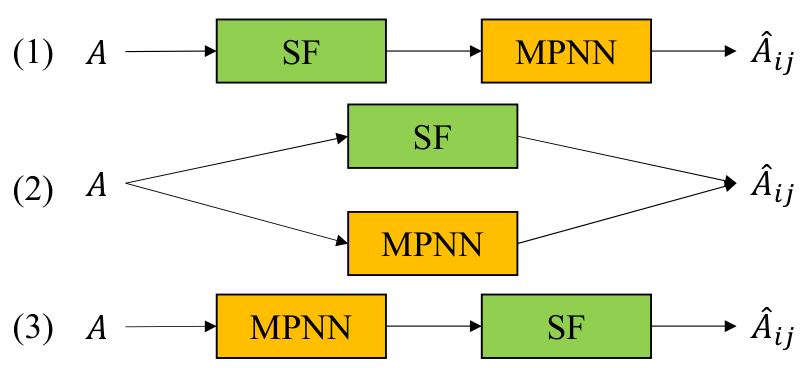
\includegraphics[width=.55\linewidth]{figures/ncnc_original_fig2.png}
\caption{NCNC 原论文第2页 Figure 2 的示意图区域摘录\cite{wang2024ncnc}：不同的结构特征与消息传递组合顺序。原图版权归原作者，保留原标签，未包含原文图注。该图描述架构类别，不是本次完整训练流程。}\label{fig:ncnc-original}
\end{figure}
\textbf{本次配置与问题。}调用固定作者的 GCN 与 \code{IncompleteCN1Predictor}；三个数据集均使用256维、一层编码、一次补全，不截断补全候选。比较完整模型与 noCNC、noCN，检验收益是否由补全或显式共同邻域产生。随机删边会使一条共同邻域证据依赖的两条边同时保留的概率下降，这是机制假设，实际贡献仍由配对消融判断。

\subsection{LPFormer：点对注意力与 PPR 上下文}
\textbf{论文与思路。}Shomer 等人的 LPFormer 发表于 KDD 2024\cite{shomer2024lpformer}。它为每个候选点对形成不同的上下文：先编码节点，再利用个性化 PageRank（PPR）筛选共同邻居、单侧邻居和较远节点，最后按节点状态及点对位置编码进行注意力聚合。PPR 的局部推送近似与经典局部图划分方法相关\cite{andersen2006ppr}。
\begin{equation}
 s_{uv}=\sum_{w\in\widehat N(u,v)}\alpha_{uvw}\,V\!\left(h_w,\mathrm{PE}(u,v,w)\right),
 \qquad \sum_{w\in\widehat N(u,v)}\alpha_{uvw}=1.
\end{equation}
这是省略多头和投影细节的示意式。作者最终将点对聚合、端点交互和类别计数送入预测头。PPR 在这里有两种作用：\emph{决定候选集合}与\emph{提供位置编码数值}，因此只将位置编码置零并不等于删除全部 PPR 信息。
\Fig{lpformer_evaluated_architecture.pdf}{1.0}{本次 LPFormer 适配器流程的重新绘制。结构攻击通过 GCN、PPR 候选、位置编码和计数共同影响输出；本报告未将这些影响拆成独立因果路径。}{fig:lpformer}
\begin{figure}[htbp]\centering
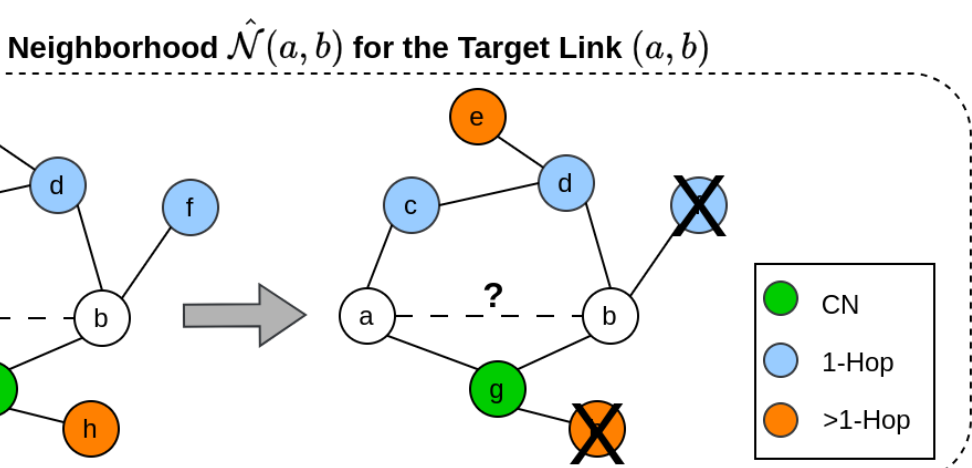
\includegraphics[width=.55\linewidth]{figures/lpformer_original_fig2_panel2.png}
\caption{LPFormer 原论文第4页 Figure 2 的第2面板局部摘录\cite{shomer2024lpformer}，展示目标点对的候选邻域筛选。原图版权归原作者；仅保留该面板，完整实际流程见图\ref{fig:lpformer}。}\label{fig:lp-original}
\end{figure}
\textbf{本次配置与问题。}调用作者 \code{LinkTransformer} 与 MLP 预测头，一层 GCN、一层点对注意力、一个注意力头；Cora/Citeseer/PubMed 的维数为128/256/128。Uniform 将注意力向量置零并冻结，候选内权重均匀，保留值投影；noPE 将位置编码输出置零，保留候选与计数。每张不同攻击图均重新计算 PPR，避免在新图上错误复用旧结构编码。训练时沿用作者全训练图 PPR，局部传播和邻域则移除当前批次目标边，因此 PPR 仍可能携带批次训练目标信息。

\subsection{Refined-GAE：较简洁传播与强解码器}
\textbf{论文与思路。}Ma 等人的 \emph{Reconsidering the Performance of GAE in Link Prediction} 发表于 CIKM 2025\cite{ma2025refined}。本文以作者代码库名 Refined-GAE 标识该工作，避免与原始 GAE 混淆。该工作强调合理选择初始表示、传播和预测器，而不把模型复杂度本身作为提升的证据。其线性邻域聚合与深度加权的思路可与 LightGCN 对照\cite{he2020lightgcn}；但作者代码中名为 \code{LightGCN} 的模块并非推荐任务原始 LightGCN 的逐行复制。

\textbf{本次实际实现。}使用已有节点属性，不新增每节点可学习 ID 嵌入，因此没有在本实验中直接检验无属性图上的正交 ID 初始化论点。首步完成归一化传播与特征投影，后续步骤共享无权重传播算子；步间使用 LayerNorm 与 dropout，各深度输出以可学习 softmax 系数加权。这里 LayerNorm 是逐节点隐藏表示归一化\cite{ba2016layernorm}，不同于输入列标准化和邻接度归一化。
\begin{equation}
 z_u=\sum_{\ell=1}^L\mathrm{softmax}(a)_\ell h_u^{(\ell)},
 \qquad f(u,v)=\mathrm{MLP}(z_u\odot z_v).
\end{equation}
Cora/Citeseer 使用4步传播和1024维；PubMed 使用2步和512维，深度参数初始为 $[1,0.5]$，随后经 softmax 并训练，不能称为固定指数权重。Cora 解码器为4层 SiLU 残差 MLP，Citeseer 为2层 ReLU MLP，PubMed 为2层 GELU MLP。
\Fig{refined_evaluated_architecture.pdf}{1.0}{本次 Refined-GAE 适配器的实际路径示意。noLN 仅删除编码器/解码器 LayerNorm；Dot 用作者点积预测器替代完整预测头，两者均独立重训。}{fig:refined}
\begin{figure}[htbp]\centering
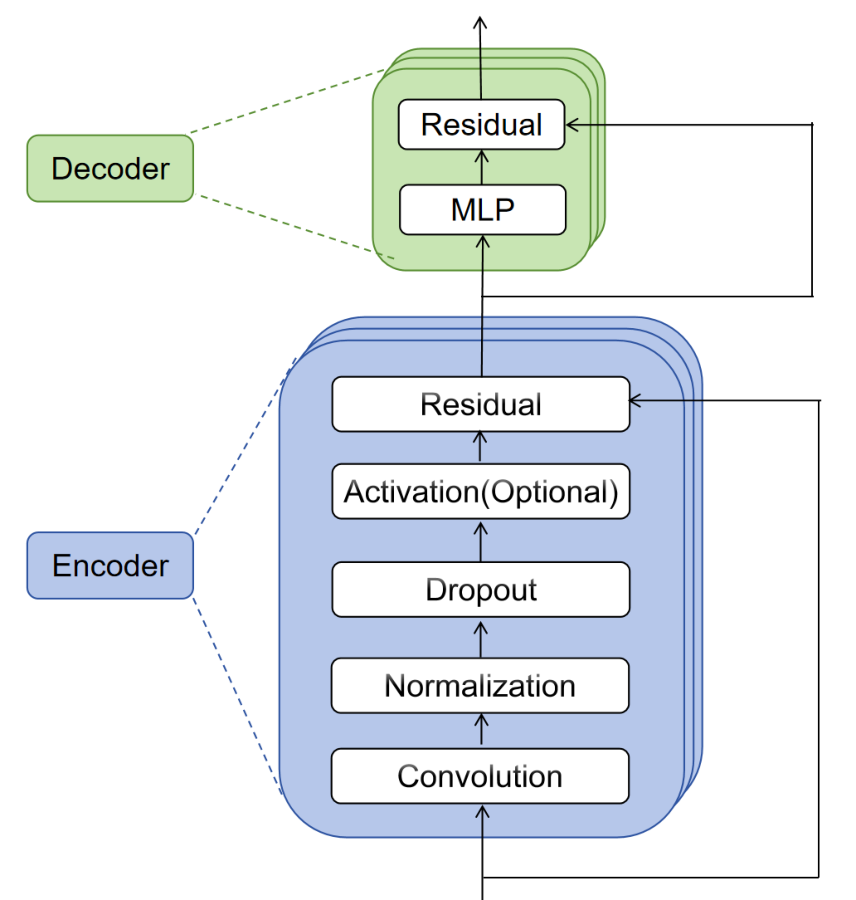
\includegraphics[height=6cm]{figures/refined_original_fig2.png}
\caption{Refined-GAE 论文 arXiv v4 第4页 Figure 2 的原示意图区域摘录\cite{ma2025refined}。这是论文对典型 GAE 编码器/解码器模块的概览，包含可选项；不是本次每个数据集具体启用项的列表。原图版权归原作者。}\label{fig:refined-original}
\end{figure}
\textbf{本次关注。}noLN 保留 dropout 以及输入与邻接归一化，用于检验网络内 LayerNorm；Dot 保留编码器架构后重新训练，用于检验完整非线性解码设计。后者同时改变参数量、非线性、正则化和训练轨迹，不能解释为在冻结编码器上只替换打分公式。

\subsection{源码版本与图像出处}
以下源码均固定提交并校验逐文件 SHA-256。报告新增图为本次独立绘制，三个原图局部的页码、裁剪范围与源 PDF 指纹保存在 \code{figure_sources.json}；Refined-GAE 引用正式2025版本，并选取对应 arXiv v4 示意图，不使用早期预印本不同的图号解释当前图。
\begin{itemize}
\item \href{https://github.com/GraphPKU/NeuralCommonNeighbor/tree/11d597013750da17ce7468e344bec756a7af39a4}{NCNC 作者代码}：\code{11d597013750da17ce7468e344bec756a7af39a4}。
\item \href{https://github.com/HarryShomer/LPFormer/tree/3ca80aba3bd1ba4903ec5c042608e4a034110c9f}{LPFormer 作者代码}：\code{3ca80aba3bd1ba4903ec5c042608e4a034110c9f}。
\item \href{https://github.com/GraphPKU/Refined-GAE/tree/5bcf00ee42134a31995bbc7bcc5359810aa99b6c}{Refined-GAE 作者代码}：\code{5bcf00ee42134a31995bbc7bcc5359810aa99b6c}。
\end{itemize}

\clearpage
\section{实验设计与可比性}
\subsection{数据、划分与属性}
三个引用网络采用 Planetoid 数据发布格式\cite{yang2016planetoid}，原始文件固定到 \code{af6abf468a772cc055bec88c52e4d6f51b7c37e3}。无向化后去除自环与重复边，保留原节点索引和属性。Cora、Citeseer、PubMed 的实际规范化统计如下；PubMed 为44324条边，和原论文表存在3条差异，沿用 main 已记录的版本。
{\small
\setlength{\tabcolsep}{3.2pt}
\renewcommand{\arraystretch}{1.10}
\begin{longtable}{lrrrrrr}
\caption{规范化数据统计与每个种子的正例划分（各划分负例数相同）}\\
\toprule
数据 & 节点 & 无向边 & 属性维数 & 训练 & 验证 & 测试 \\
\midrule
\endfirsthead
\multicolumn{7}{l}{规范化数据统计与每个种子的正例划分（各划分负例数相同）（续）}\\
\toprule
数据 & 节点 & 无向边 & 属性维数 & 训练 & 验证 & 测试 \\
\midrule
\endhead
\midrule\multicolumn{7}{r}{续下页}\\
\endfoot
\bottomrule
\endlastfoot
Cora & 2708 & 5278 & 1433 & 4222 & 264 & 792 \\
Citeseer & 3327 & 4552 & 3703 & 3641 & 228 & 683 \\
PubMed & 19717 & 44324 & 500 & 35459 & 2216 & 6649 \\
\end{longtable}
}

对每个种子0、1、2生成一次80\%/5\%/15\%正边划分。训练、验证、测试负例数量分别与其正例相等，均为完整干净图中不存在的无向非自环点对，三组负例互斥。不同模型和组件共享同种子的数据划分；不按模型性能挑图或重抽负例。

M 使用 main 的数据加载、划分、\code{node_feature_matrix} 逐属性列标准化，以及 \code{_cap_pairs}：按固定顺序取测试正负例各前500个。每次评估1000个点对，绝非按分数选最高的500个。P 使用原始属性并对完整测试候选计分：Cora 每类792个，Citeseer 每类683个。两轮输入不同，所以 M 的81组权重全部从头训练，没有复用 P 的54组权重。DICE 可读取类别标签以选择攻击边；预测模型不读取这些标签。

\subsection{训练目标、目标边移除与选点}
所有模型与变体均独立训练。正例 minibatch 为512，负例与正例按固定划分一一配对，采用 logits 形式的二元交叉熵：
\begin{equation}
 \mathcal L=-\frac1{2B}\left[\sum_{i=1}^B\log\sigma(f(u_i,v_i))+\sum_{j=1}^B\log(1-\sigma(f(\bar u_j,\bar v_j)))\right].
\end{equation}
训练传播图只含训练正边，并移除当前批次全部目标正边；梯度范数裁剪上限为1。采用共享 batch512 是为了在目标移除后保留非空训练上下文；例如 Citeseer 的3641条训练边不足以支撑作者4096条正例全批移除。作者原始批量、负采样数、训练轮次与本文有明确差别。

M 最多训练100轮，每10轮用干净验证 AUC 选点，30轮未提升停止；完整保留 main 节点对基线实际使用的 \emph{train+validation 图上下文}，因此验证正边在验证传播图中可见。这是协议限制，较高的验证 AUC 不应解释为对未见边的泛化证明。P 则每5轮在\emph{只含训练边}的上下文验证，同样最多100轮、耐心30轮。测试正边在所有推理图中移除，模型权重在攻击推理前冻结。

NCNC 使用编码器/预测器分组学习率；LPFormer 使用作者的指数学习率因子；Refined-GAE 在 Cora 使用 AdamW，其余采用 Adam。各作者数据集专属配置保留，未额外用测试性能调参，因此跨模型差异也包含优化配方的影响。
{\footnotesize
\setlength{\tabcolsep}{3.2pt}
\renewcommand{\arraystretch}{1.10}
\begin{longtable}{llrrrrrr}
\caption{主训练配置；统一采用 batch512，dropout 指预测器/共享配置（详见正文）}\\
\toprule
数据 & 模型 & 维数 & dropout & 学习率 & 衰减项 & LR因子 & 作者batch \\
\midrule
\endfirsthead
\multicolumn{8}{l}{主训练配置；统一采用 batch512，dropout 指预测器/共享配置（详见正文）（续）}\\
\toprule
数据 & 模型 & 维数 & dropout & 学习率 & 衰减项 & LR因子 & 作者batch \\
\midrule
\endhead
\midrule\multicolumn{8}{r}{续下页}\\
\endfoot
\bottomrule
\endlastfoot
Cora & NCNC & 256 & 0.05 & 0.0043/0.0024 & 0.0 & 1.0 & 1152 \\
Cora & LPFormer & 128 & 0.1 & 0.005 & 0.0 & 0.975 & 1024 \\
Cora & Refined-GAE & 1024 & 0.6 & 0.005 & 0.01 & 1.0 & 2048 \\
Citeseer & NCNC & 256 & 0.55 & 0.0085/0.0078 & 0.0 & 1.0 & 384 \\
Citeseer & LPFormer & 256 & 0.1 & 0.005 & 0.0 & 0.95 & 1024 \\
Citeseer & Refined-GAE & 1024 & 0.6 & 0.001 & 0.0 & 1.0 & 4096 \\
PubMed & NCNC & 256 & 0.05 & 0.0097/0.002 & 0.0 & 1.0 & 2048 \\
PubMed & LPFormer & 128 & 0.3 & 0.001 & 0.0001 & 1.0 & 1024 \\
PubMed & Refined-GAE & 512 & 0.4 & 0.001 & 0.0 & 1.0 & 4096 \\
\end{longtable}
}

该表的 dropout 是预测器或共享配置，不能替代各路径的全部 dropout。NCNC 的 GCN dropout 为 Cora0.05、Citeseer0.75、PubMed0.1；输入 dropout 为0.7/0.4/0.3，尾部为0.3/0/0，预测器为0.05/0.55/0.05。Cora 的预测器边 dropout 另为0.4，其余为0。NCNC 的补全校准 $(\mathrm{pt},\mathrm{scale},\mathrm{offset},\alpha)$ 分别是 Cora $(0.75,4.3,2.8,1)$、Citeseer $(0.75,6.5,4.4,0.4)$、PubMed $(0.5,5.3,0.5,0.3)$。

LPFormer 的 PPR 参数 $\alpha=0.15$，误差阈值为 Cora/Citeseer $10^{-7}$、PubMed $10^{-5}$；单侧候选阈值0.01，较远候选阈值为 Cora/PubMed0.01、Citeseer1.0。Refined-GAE 的传播深度、预测器激活和残差设置见上一节。源包 \code{data/main/run_manifest.json} 提供81组完整运行配置及作者来源，P 对应 manifest 独立保存。

\subsection{M：固定 main 的攻击与缓存}
直接调用固定 main 的 \code{apply_attack}，在\emph{完整干净图}上生成结构扰动，再删除\emph{全部}测试正边，得到推理图：
\begin{equation}
 E^{\rm raw}_{a,r,s}=\mathcal A_a(E,r,s),\quad
 E^{\rm infer}_{a,r,s}=E^{\rm raw}_{a,r,s}\setminus E^{+}_{\rm test,s},\quad
 b=\operatorname{round}(r|E|).
\end{equation}
所有模型和组件使用同一 $E^{\rm infer}$；不为某模型重新优化攻击。$r$ 取0.1、0.25、0.5，clean 为额外条件。预算是编辑次数相对于完整图边数的比例，\textbf{50\%混合编辑预算不等于删掉一半边}。
\begin{itemize}
\item \textbf{RF}：随机删除约半预算，再随机插入其余预算；原实现可能重新插入刚删的边，所以实际差集编辑数可小于请求预算。本文保留此行为并单独记录实际数值。
\item \textbf{DICE}：优先采用类别标签作为社区，删同社区边、插跨社区边，约一半删除、一半插入。该攻击使用额外标签知识，与不使用标签的 RF/EA 的威胁信息不同。
\item \textbf{EA}：main 的32维单层线性节点嵌入代理，拟合60步，每步2048正例和2048随机节点对；后者不是严格过滤后的非边。冻结代理权重后，对邻接求一次梯度，分别选取约半预算删除和插入。原函数注释使用“meta-gradient”措辞，但实际没有反向展开60步优化；应解释为固定代理的邻接梯度排序。
\end{itemize}
原 SGDiff 论文的嵌入攻击关联 Bojchevski 与 G\"unnemann 的图投毒方法，并调用 DeepRobust\cite{bojchevski2019attack,li2020deeprobust}。\textbf{main 的线性代理实现不是该谱/NetMF攻击的原样实现。}因此本轮是对齐\emph{仓库代码}，不是声称复现原论文 DeepRobust 的 EA 表。对训练好的三个目标模型仅扰动推理图，属于迁移式 evasion 评估，既不是三个模型各自的白盒最强攻击，也不是重新训练目标模型的投毒实验。

PubMed 有19717节点，超过 main 密集 EA 的 \code{EA_MAX_NODES=4000}，三种子均按协议跳过。M 总共保存81张共享图（含9张clean）及9份划分，保留 \code{raw_edges} 与 \code{edges} 两层边表；模型推理必须用后者。测试负例未受到额外保护，某些计分负例可能被攻击插入；附录如实列出数量。这种情况影响指标解释，不能悄悄修改攻击后仍声称使用原协议。

图缓存是这次用固定代码新生成的，不保证与历史 main/H20 或合作者环境的旧缓存逐边相同。共享算法名称与种子还不足以合表；必须共享边表、测试点对或验证指纹。历史18张 P 协议 EA 图已另行归档，不作为本轮 M 的 EA 图。

\subsection{P：候选保护与额外机制探针}
P 在移除测试正边的 train+val 可见图上攻击，预算分母也用该图边数；保护所有测试正负候选及验证负例。RF/DICE 的删插预算固定；EA 则采用统一的合法翻转梯度排序，而不是 main 的删插半配额。本轮旧18张 EA 图经实际差集审计\textbf{全部为插边}，不能用它们证明抵抗删边。

在 clean、RF/DICE/EA三档之外，P 另外评估随机纯删边50\%、按节点度加权删边50\%、纯插边50\%及属性行置换，共14条件。属性置换保持特征集合与图结构，打乱属性对应节点；不等于去掉属性或重新训练结构-only。按度加权删边也不等同于专门寻找最危险边的最优攻击。M 未运行这些额外探针；PubMed 的探针结果因而不存在，不以 Cora/Citeseer 代替。

\subsection{组件消融的操作与解释}
\begin{table}[htbp]\centering\small
\caption{每模型两个变体；全部独立重训。表与附录统一使用简短标签。}\label{tab:ablations}
\begin{tabular}{lp{3.8cm}p{6.0cm}}\toprule
变体&操作&保留内容与解释边界\\\midrule
noCNC&NCNC 补全深度1改0&保留共同邻域聚合，相当于本配置下 NCN\\
noCN&NCNC 使用作者CN0预测器&保留 GCN$(A,X)$；不是特征-only\\
Uniform&LPFormer 注意力向量置零冻结&保留候选、值投影、位置编码和计数\\
noPE&LPFormer 位置编码输出置零&保留 PPR 候选筛选、类别划分与计数\\
noLN&Refined-GAE LayerNorm改恒等&保留 dropout、输入标准化、邻接归一化\\
Dot&Refined-GAE 改作者点积预测器&编码器架构保留，全部参数独立重训\\\bottomrule
\end{tabular}\end{table}
模型结构改变会影响参数初始化和训练轨迹；共享种子不意味着逐参数严格匹配。配对设计控制数据、图和候选，不能排除参数量、优化难度、正则化的共同影响。

\subsection{指标、配对差值与统计口径}
主指标 AUC 与 AP 调用 main 的实际指标函数。AUC 衡量正例相对负例的排序，AP 反映精确率与召回率的综合排序表现；二者受测试候选与负例难度影响。补充排名指标明确区分：
\begin{equation}
 P_{100}=\frac{\#\{\text{合并正负候选最高100分中的正例}\}}{100},\quad
 H_{100}=\frac1{n_+}\sum_i\mathbf1\{s_i^+>s^-_{(100)}\}.
\end{equation}
$s^-_{(100)}$ 为固定全局负池第100高分。main 历史名 \code{hit@100} 实际为 $P_{100}$，并列分数沿输入次序处理；M 还记录并列平均 $\bar P_{100}$。此处 $H_{100}$ 不是对所有可能非边排名的指标，也不等同于不同论文/OGB配置下的 Hits@100。

每个设置报告三个种子的均值与\emph{样本标准差}（ddof=1），不把标准差写成置信区间。鲁棒性同时看攻击后绝对精度 $m_a$ 和同种子降幅 $D_s=m_{s,\rm clean}-m_{s,a}$。组件效应为 $C_s=m_{s,\rm full}-m_{s,\rm variant}$，并额外报告 $D_{s,\rm variant}-D_{s,\rm full}$。所有差值先配对再求标准差；没有进行显著性检验，三个种子不足以支持普遍机制结论。

\clearpage
\begin{landscape}
\section{main 协议实验结果}
\subsection{综合图：完整模型、攻击预算与组件效应}
图\ref{fig:m-heat}--\ref{fig:m-component}展示完整网格。灰格表示未运行，误差棒为样本标准差；附录提供对应数值。
\begin{figure}[H]\centering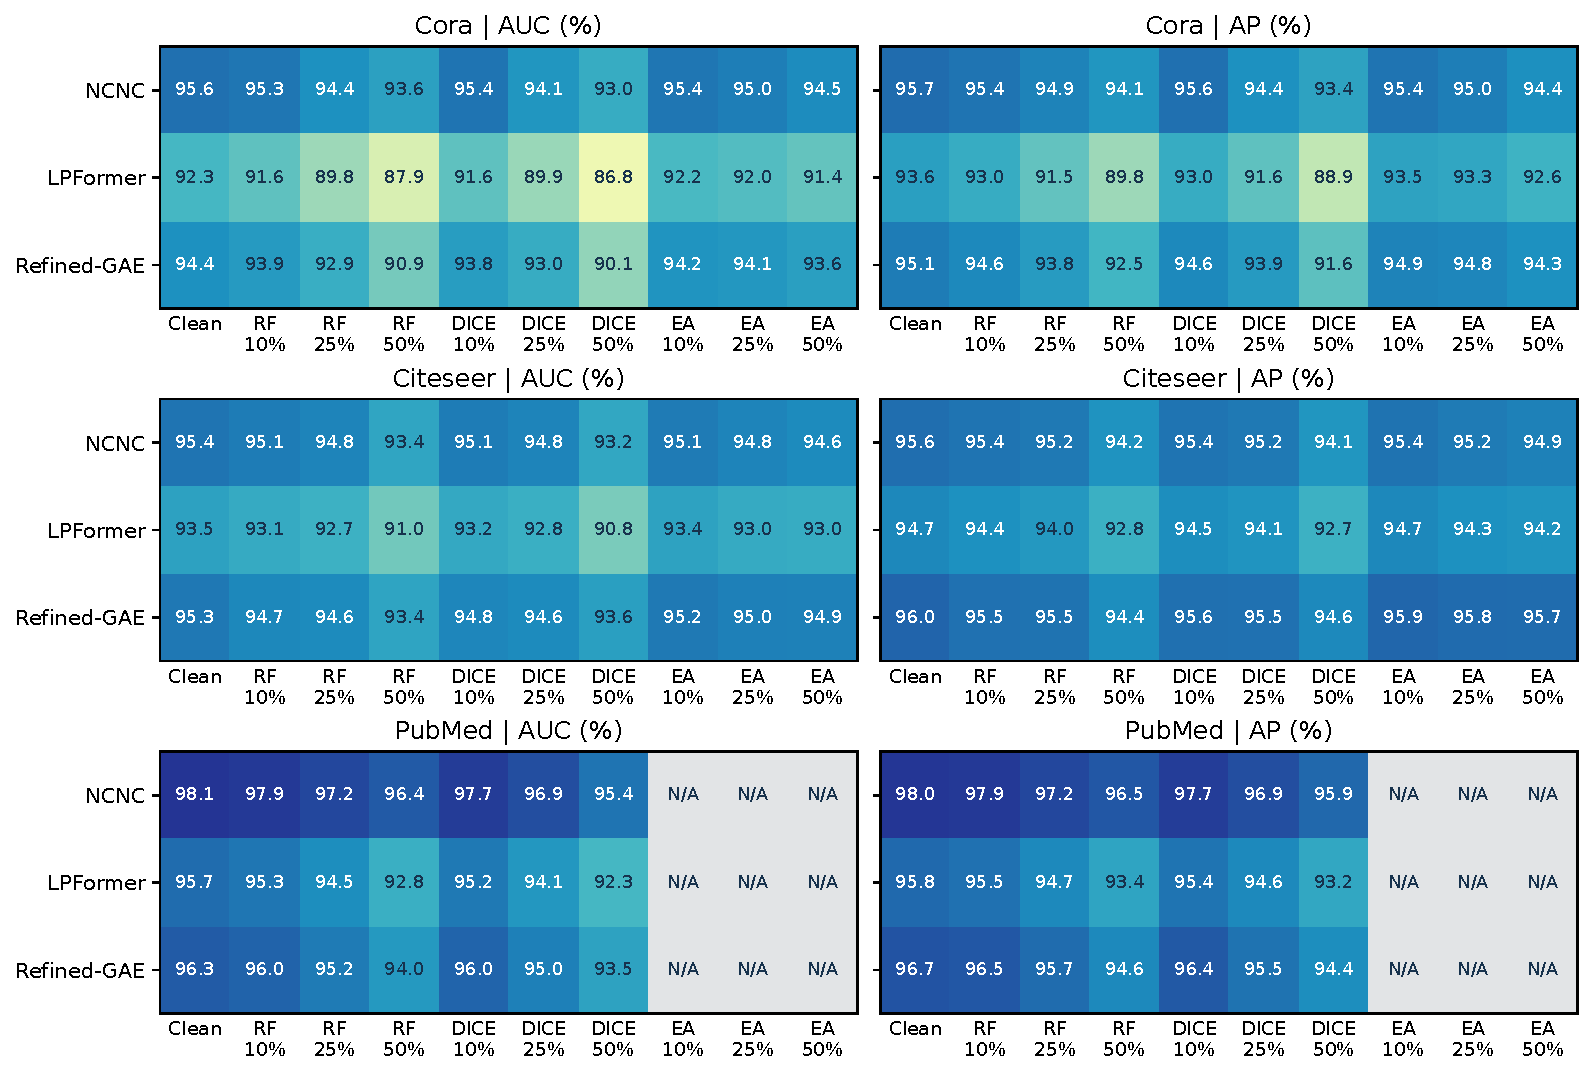
\includegraphics[width=23cm,height=11cm,keepaspectratio]{figures/main_full_models.pdf}\caption{M 协议：三个数据集完整模型的全部 AUC/AP 均值。PubMed EA 因节点上限跳过，其他 RF/DICE 三档及全部组件已运行。}\label{fig:m-heat}\end{figure}
\clearpage
\begin{figure}[H]\centering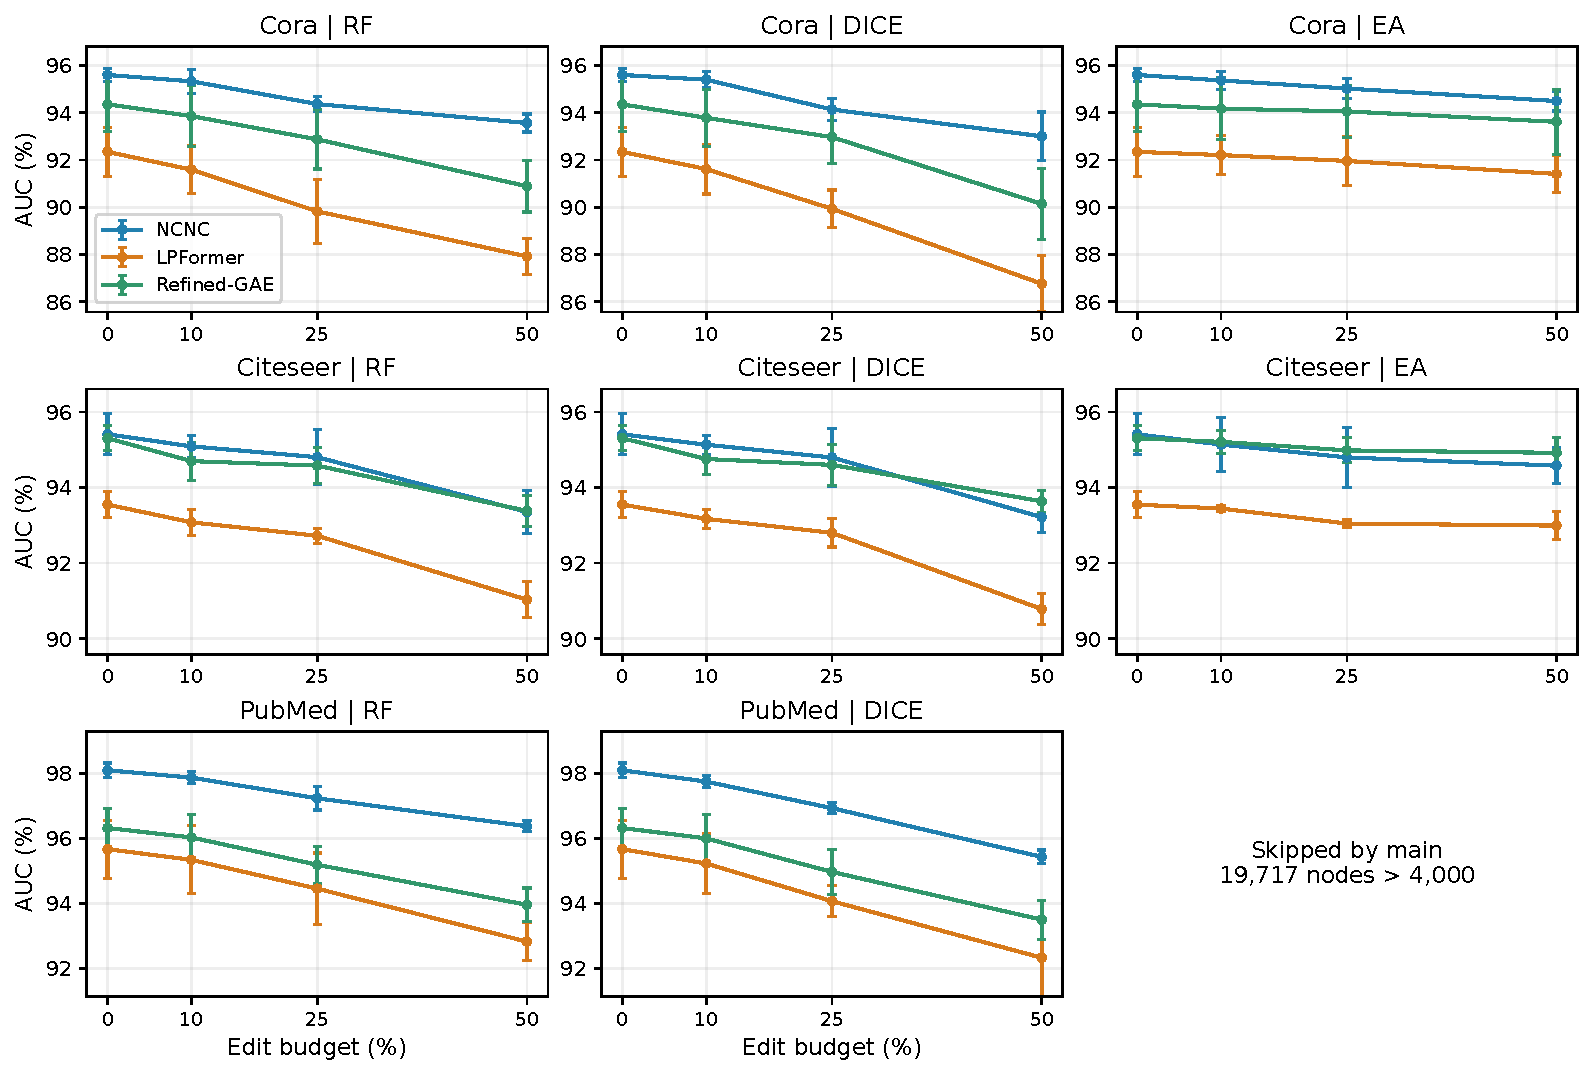
\includegraphics[width=23cm,height=14cm,keepaspectratio]{figures/main_attack_curves.pdf}\caption{M 协议：RF、DICE、EA 的预算曲线，均值与样本标准差。预算为完整图边数的混合编辑比例；不是纯删边比例。EA 的相对影响小只说明该代理攻击的迁移效果，不能推出对最强攻击安全。}\label{fig:m-curves}\end{figure}
\end{landscape}
\clearpage
\begin{figure}[H]\centering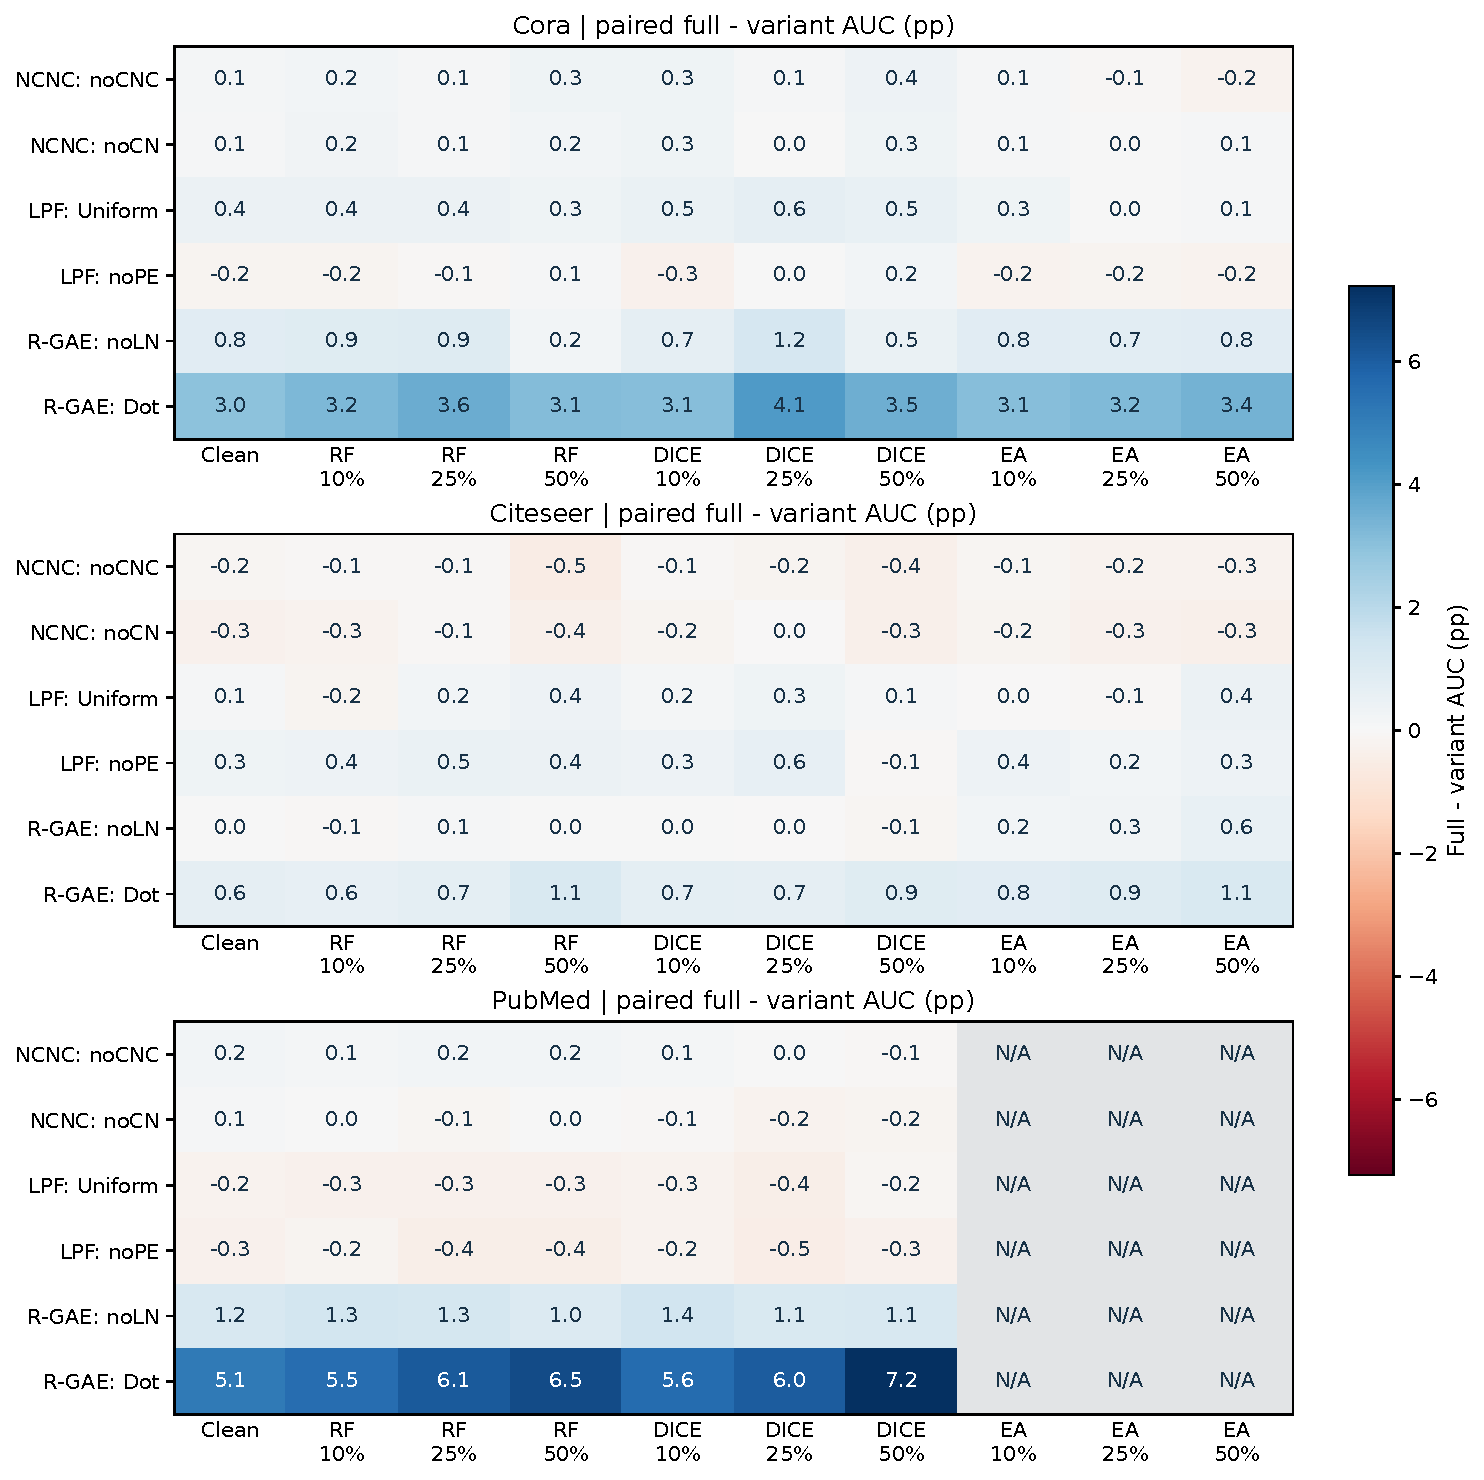
\includegraphics[width=\linewidth,height=.88\textheight,keepaspectratio]{figures/main_component_effects.pdf}\caption{M 协议：完整模型减去组件变体的配对 AUC（百分点）。正值为完整模型更高，负值为变体更高。每个变体独立重训；此图不是显著性检验。}\label{fig:m-component}\end{figure}
\clearpage
\subsection{完整模型：干净精度与攻击后精度}
{\small
\setlength{\tabcolsep}{3.2pt}
\renewcommand{\arraystretch}{1.10}
\begin{longtable}{llrrrr}
\caption{main 协议：完整模型 AUC（百分数）}\\
\toprule
数据 & 模型 & Clean & RF50 & DICE50 & EA50 \\
\midrule
\endfirsthead
\multicolumn{6}{l}{main 协议：完整模型 AUC（百分数）（续）}\\
\toprule
数据 & 模型 & Clean & RF50 & DICE50 & EA50 \\
\midrule
\endhead
\midrule\multicolumn{6}{r}{续下页}\\
\endfoot
\bottomrule
\endlastfoot
Cora & NCNC & $95.60\pm0.26$ & $93.57\pm0.38$ & $93.01\pm1.03$ & $94.50\pm0.42$ \\
Cora & LPFormer & $92.35\pm1.03$ & $87.92\pm0.76$ & $86.76\pm1.18$ & $91.41\pm0.79$ \\
Cora & Refined-GAE & $94.36\pm1.14$ & $90.89\pm1.09$ & $90.14\pm1.49$ & $93.62\pm1.37$ \\
Citeseer & NCNC & $95.41\pm0.54$ & $93.35\pm0.56$ & $93.22\pm0.40$ & $94.58\pm0.47$ \\
Citeseer & LPFormer & $93.55\pm0.35$ & $91.03\pm0.47$ & $90.78\pm0.42$ & $92.99\pm0.37$ \\
Citeseer & Refined-GAE & $95.31\pm0.33$ & $93.38\pm0.41$ & $93.64\pm0.29$ & $94.92\pm0.40$ \\
PubMed & NCNC & $98.09\pm0.22$ & $96.37\pm0.17$ & $95.43\pm0.21$ & N/A \\
PubMed & LPFormer & $95.66\pm0.89$ & $92.82\pm0.59$ & $92.32\pm1.22$ & N/A \\
PubMed & Refined-GAE & $96.32\pm0.61$ & $93.95\pm0.52$ & $93.50\pm0.60$ & N/A \\
\end{longtable}
}

\textbf{Cora。}NCNC 的干净 AUC 为 $95.60\pm0.26$，RF50、DICE50 后为 $93.57\pm0.38$、$93.01\pm1.03$，配对平均降幅2.03、2.60个百分点。LPFormer 对应降幅4.43、5.58，Refined-GAE为3.47、4.21。本次设置下，NCNC 在这两类扰动上同时具有较高攻击后均值与较小降幅；但此排名不是补全机制的因果证据，见后续消融。

\textbf{Citeseer。}干净均值为 NCNC95.41、Refined-GAE95.31、LPFormer93.55。DICE50 下 Refined-GAE 为 $93.64\pm0.29$，高于 NCNC 的 $93.22\pm0.40$；其平均降幅1.67也小于NCNC的2.19。EA50 下 Refined-GAE 为 $94.92\pm0.40$，也高于 NCNC 的 $94.58\pm0.47$。因此不能把 Cora 上的模型顺序概括成所有数据集通用的鲁棒性排名。

\textbf{PubMed。}NCNC 的干净、RF50、DICE50 AUC 分别为 $98.09\pm0.22$、$96.37\pm0.17$、$95.43\pm0.21$。LPFormer 对应为 $95.66\pm0.89$、$92.82\pm0.59$、$92.32\pm1.22$；Refined-GAE 为 $96.32\pm0.61$、$93.95\pm0.52$、$93.50\pm0.60$。NCNC 在该数据集这三条件均值最高。其 RF50/DICE50 平均降幅约1.72/2.67个百分点；LPFormer为2.84/3.34，Refined-GAE为2.36/2.82。所有三种子的原始值见附录，并未将三种子波动解释为统计显著性。

\textbf{攻击类型的解释。}Cora/Citeseer 中，EA50 的精度降幅通常小于 RF/DICE50。该现象只说明本次固定线性代理、删插配额、输入和采样下的迁移效果；代理目标可能与三个模型的薄弱点不一致。DICE 使用类别信息，因此也不能仅按降幅大小断言它是同信息预算下的最强攻击。

\subsection{配对消融：哪些机制受到数据支持}
{\footnotesize
\setlength{\tabcolsep}{3.2pt}
\renewcommand{\arraystretch}{1.10}
\begin{longtable}{lllrrrr}
\caption{M 协议组件效应：完整模型减变体 AUC（百分点）}\\
\toprule
数据 & 模型 & 变体 & Clean & RF50 & DICE50 & EA50 \\
\midrule
\endfirsthead
\multicolumn{7}{l}{M 协议组件效应：完整模型减变体 AUC（百分点）（续）}\\
\toprule
数据 & 模型 & 变体 & Clean & RF50 & DICE50 & EA50 \\
\midrule
\endhead
\midrule\multicolumn{7}{r}{续下页}\\
\endfoot
\bottomrule
\endlastfoot
Cora & NCNC & noCN & $0.09\pm0.51$ & $0.22\pm0.30$ & $0.32\pm0.71$ & $0.07\pm0.56$ \\
Cora & NCNC & noCNC & $0.14\pm0.52$ & $0.31\pm0.19$ & $0.37\pm0.51$ & $-0.25\pm0.25$ \\
Cora & LPFormer & noPE & $-0.21\pm0.56$ & $0.10\pm1.10$ & $0.21\pm1.16$ & $-0.23\pm0.38$ \\
Cora & LPFormer & Uniform & $0.43\pm1.23$ & $0.32\pm1.04$ & $0.52\pm1.30$ & $0.06\pm0.41$ \\
Cora & Refined-GAE & Dot & $2.98\pm0.98$ & $3.11\pm1.69$ & $3.52\pm1.95$ & $3.41\pm1.21$ \\
Cora & Refined-GAE & noLN & $0.80\pm0.79$ & $0.23\pm0.99$ & $0.47\pm1.24$ & $0.82\pm0.68$ \\
Citeseer & NCNC & noCN & $-0.31\pm0.32$ & $-0.39\pm0.22$ & $-0.35\pm0.33$ & $-0.35\pm0.10$ \\
Citeseer & NCNC & noCNC & $-0.15\pm0.35$ & $-0.51\pm0.19$ & $-0.38\pm0.50$ & $-0.25\pm0.17$ \\
Citeseer & LPFormer & noPE & $0.33\pm0.44$ & $0.45\pm0.57$ & $-0.07\pm0.18$ & $0.34\pm0.42$ \\
Citeseer & LPFormer & Uniform & $0.09\pm0.32$ & $0.37\pm0.31$ & $0.10\pm0.39$ & $0.44\pm0.43$ \\
Citeseer & Refined-GAE & Dot & $0.64\pm0.35$ & $1.13\pm0.52$ & $0.89\pm0.54$ & $1.11\pm0.60$ \\
Citeseer & Refined-GAE & noLN & $0.02\pm0.31$ & $0.04\pm0.64$ & $-0.14\pm0.58$ & $0.55\pm0.08$ \\
PubMed & NCNC & noCN & $0.07\pm0.36$ & $0.04\pm0.39$ & $-0.20\pm0.53$ & N/A \\
PubMed & NCNC & noCNC & $0.21\pm0.37$ & $0.21\pm0.29$ & $-0.11\pm0.44$ & N/A \\
PubMed & LPFormer & noPE & $-0.31\pm0.41$ & $-0.42\pm0.82$ & $-0.33\pm0.75$ & N/A \\
PubMed & LPFormer & Uniform & $-0.23\pm0.59$ & $-0.33\pm0.60$ & $-0.15\pm0.70$ & N/A \\
PubMed & Refined-GAE & Dot & $5.09\pm0.36$ & $6.47\pm0.94$ & $7.23\pm1.08$ & N/A \\
PubMed & Refined-GAE & noLN & $1.18\pm0.45$ & $0.98\pm0.69$ & $1.13\pm0.62$ & N/A \\
\end{longtable}
}

\textbf{NCNC：补全的边际收益较小且方向不稳定。}完整模型减 noCNC 的干净图差为 Cora $0.14\pm0.52$、Citeseer $-0.15\pm0.35$、PubMed $0.21\pm0.37$ 个百分点。完整模型的攻击表现不能直接归因于一次共同邻居补全。noCN 还保留结构传播，故其较小性能差不说明结构没有作用。当前结果更适合表述为：在作者超参数和统一训练预算下，端点编码分支已能保留相当一部分判别信息。

\textbf{LPFormer：学习注意力与位置编码并非稳定提升。}PubMed 上完整模型减 Uniform 的干净配对差为 $-0.23\pm0.59$，减 noPE 为 $-0.31\pm0.41$；DICE50 下完整减 noPE 为 $-0.33\pm0.75$。均值方向提示该设置中复杂组件未稳定带来收益，但三种子不能证明组件普遍无效。noPE 仍使用 PPR 筛选，不能以此推断模型不需要结构上下文。

\textbf{Refined-GAE：PubMed 的解码器选择影响较大。}完整模型减 Dot 的干净 AUC 为 $5.09\pm0.36$，DICE50 为 $7.23\pm1.08$ 个百分点。说明完整解码设计在本次 PubMed 设置下有明显的数值收益；该比较同时反映参数量、非线性、正则化及重新训练后的编码差异。它支持进一步检查点积几何表达的限制，不支持把全部差距归因于某个孤立的激活函数。

\subsection{与 main 已有 PubMed 结果的关系}
main 的 README、\code{docs/reproduction.md} 和 \code{results/sgdiff-paper-v2/} 已有 SGDiff PubMed 10种子结果，AUC 约 $0.902\pm0.002$，以及涉及 PubMed 的迁移记录。\code{configs/sgdiff_pubmed.yaml} 的1-hop、每跳20、结构扩散10步、特征64维两层/扩散50步、50训练轮和10预训练轮是 SGDiff 专属设置，不能套给这三个架构。

这些历史 SGDiff 结果与本文的种子数、候选规模、图缓存和训练配方不同。本文没有将 SGDiff 的0.902与三个新模型的均值作直接胜负比较，也没有用现有结果代替同图重跑。main 的 EA 节点上限是本次实现约束；原 SGDiff 论文包含 PubMed 鲁棒性表，二者必须区分。

\clearpage
\begin{landscape}
\section{候选保护协议的补充机制实验}
本节数值均来自P协议；与M同时改变属性、验证图、候选和攻击过程，不能将两轮差值仅归因于EA。
\begin{figure}[H]\centering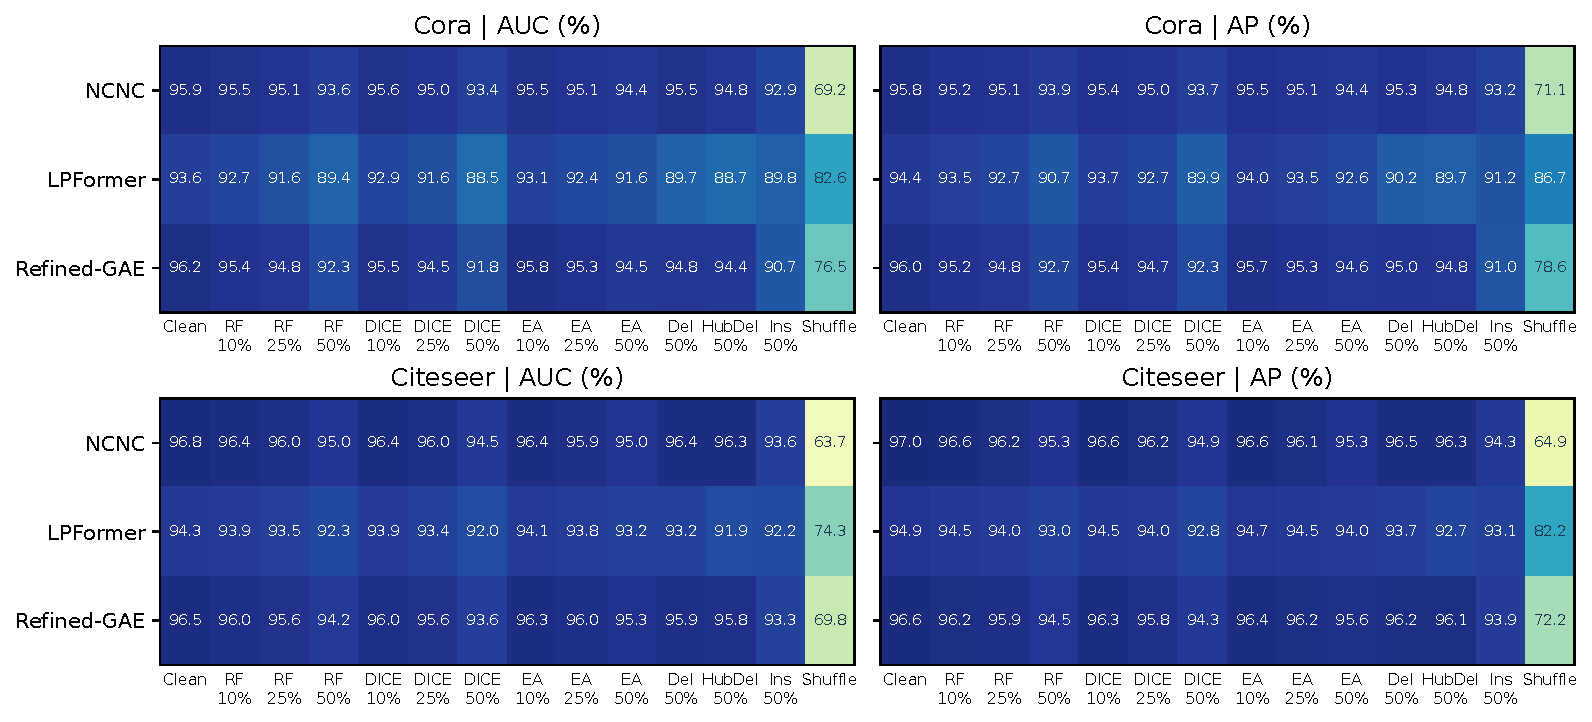
\includegraphics[width=23cm,height=11cm,keepaspectratio]{figures/protected_performance_overview.pdf}\caption{P 协议：完整模型在全部14条件下的 AUC/AP 均值。EA 列的18张实际图均为插边，不代表同时经历删边。}\label{fig:p-overview}\end{figure}
\clearpage
\begin{figure}[H]\centering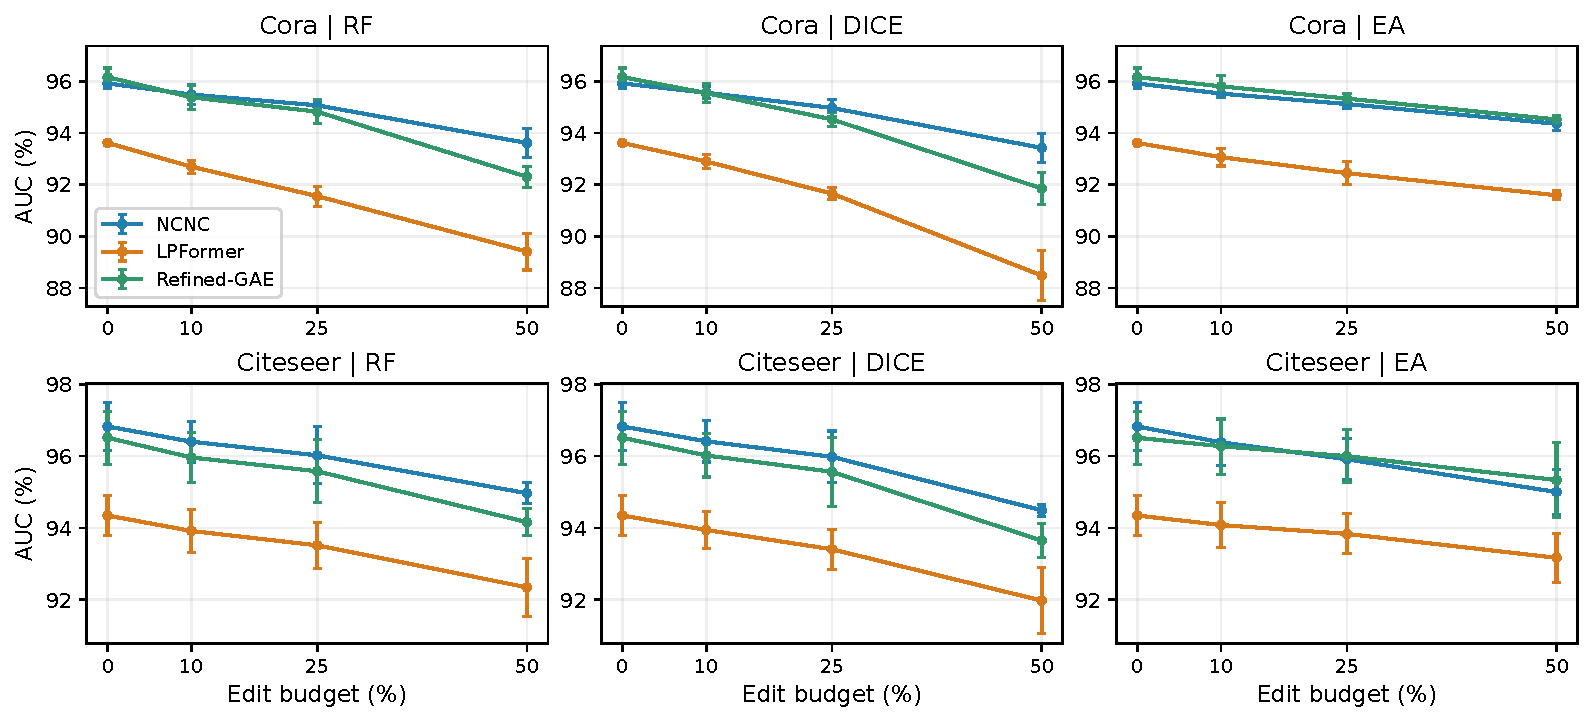
\includegraphics[width=23cm,height=14cm,keepaspectratio]{figures/protected_attack_curves.pdf}\caption{P 协议：RF/DICE/EA 多档预算的 AUC 曲线。此处的预算分母和候选保护规则与 M 不同，不能把两图曲线合并作攻击算法的单变量比较。}\label{fig:p-curves}\end{figure}
\clearpage
\begin{figure}[H]\centering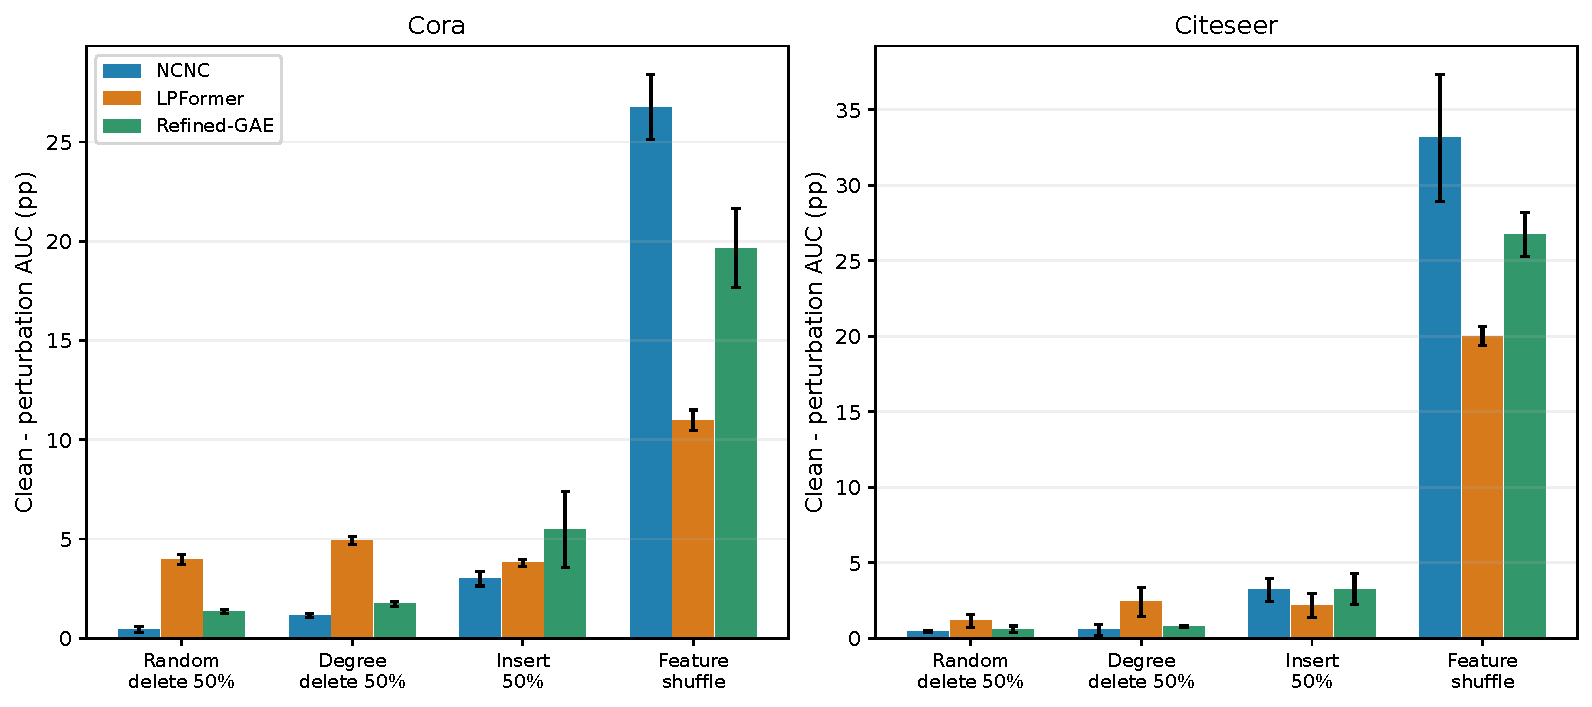
\includegraphics[width=23cm,height=14cm,keepaspectratio]{figures/protected_probe_damage.pdf}\caption{P 协议：纯删边、按度删边、插边和属性置换的配对损失。正降幅表示退化。属性置换检验冻结模型的属性错配敏感性，不是结构-only 重训。}\label{fig:p-probe}\end{figure}
\clearpage
\begin{figure}[H]\centering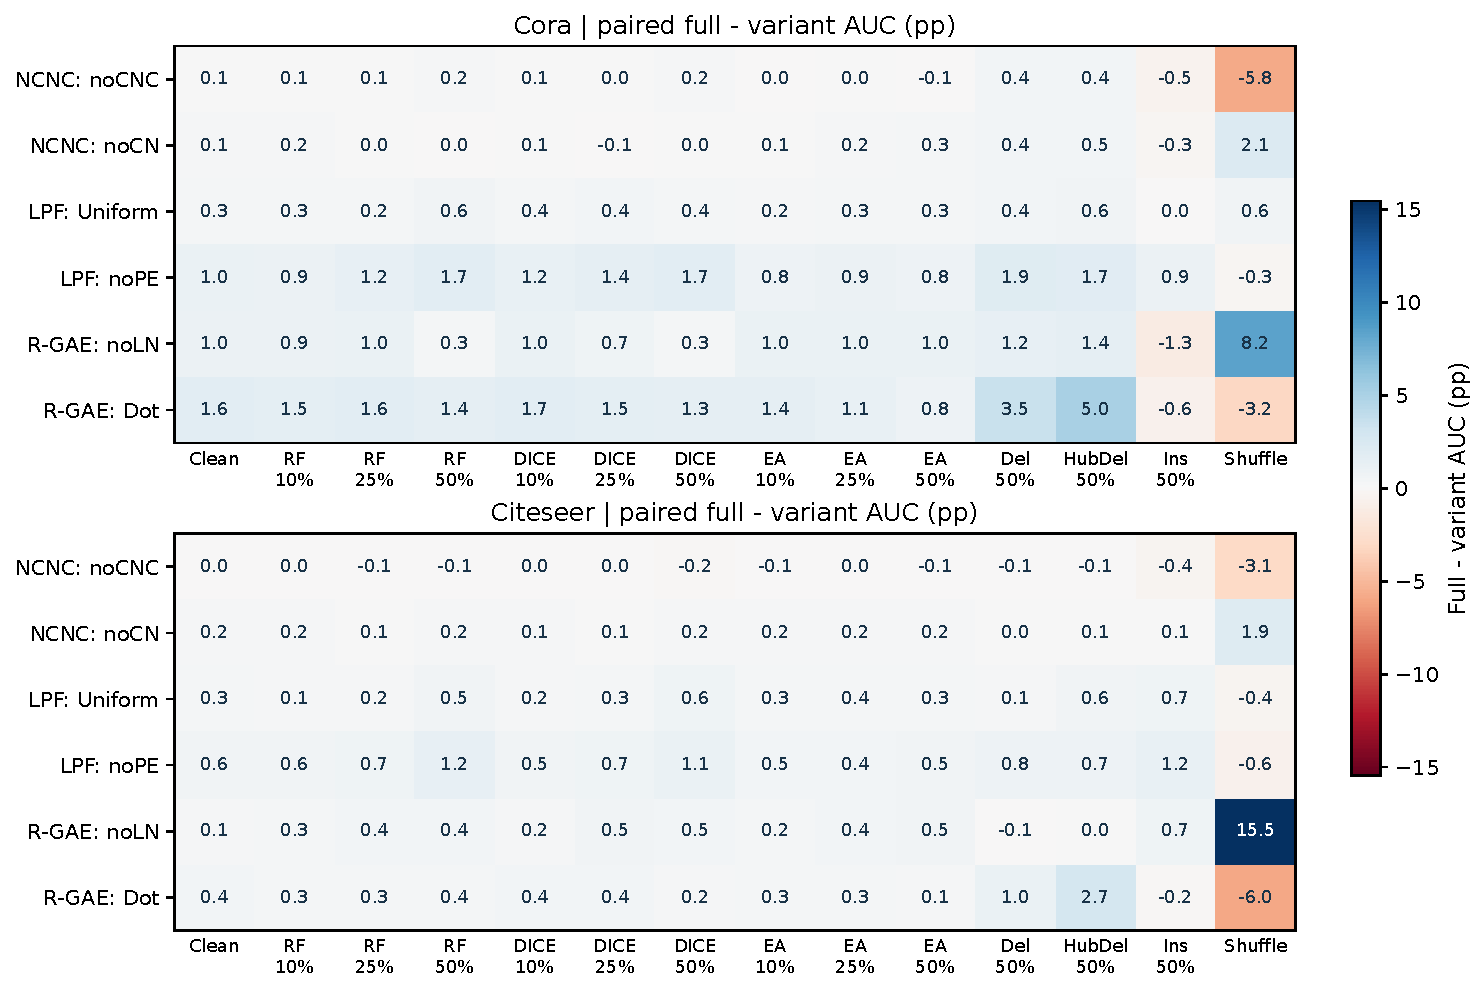
\includegraphics[width=23cm,height=14cm,keepaspectratio]{figures/protected_component_effects.pdf}\caption{P 协议：全部组件的配对效应。与 M 分开报告，检查机制观察是否依赖协议。}\label{fig:p-component}\end{figure}
\end{landscape}
\subsection{纯删边、集中删边与属性错配}
{\footnotesize
\setlength{\tabcolsep}{3.2pt}
\renewcommand{\arraystretch}{1.10}
\begin{longtable}{llrrrrr}
\caption{P 协议完整模型的干净与机制探针 AUC（百分数）}\\
\toprule
数据 & 模型 & Clean & Del50 & HubDel50 & Ins50 & Shuffle \\
\midrule
\endfirsthead
\multicolumn{7}{l}{P 协议完整模型的干净与机制探针 AUC（百分数）（续）}\\
\toprule
数据 & 模型 & Clean & Del50 & HubDel50 & Ins50 & Shuffle \\
\midrule
\endhead
\midrule\multicolumn{7}{r}{续下页}\\
\endfoot
\bottomrule
\endlastfoot
Cora & NCNC & $95.92\pm0.19$ & $95.47\pm0.14$ & $94.77\pm0.31$ & $92.92\pm0.55$ & $69.16\pm1.69$ \\
Cora & LPFormer & $93.61\pm0.08$ & $89.67\pm0.23$ & $88.70\pm0.12$ & $89.82\pm0.25$ & $82.63\pm0.58$ \\
Cora & Refined-GAE & $96.16\pm0.35$ & $94.80\pm0.42$ & $94.43\pm0.25$ & $90.70\pm1.58$ & $76.52\pm1.64$ \\
Citeseer & NCNC & $96.83\pm0.67$ & $96.40\pm0.60$ & $96.27\pm0.77$ & $93.62\pm0.48$ & $63.69\pm3.74$ \\
Citeseer & LPFormer & $94.35\pm0.55$ & $93.20\pm0.71$ & $91.93\pm1.52$ & $92.17\pm0.30$ & $74.34\pm0.39$ \\
Citeseer & Refined-GAE & $96.51\pm0.73$ & $95.90\pm0.60$ & $95.75\pm0.80$ & $93.27\pm0.67$ & $69.80\pm0.72$ \\
\end{longtable}
}

NCNC 在随机纯删边50\%下，Cora/Citeseer 的 AUC 分别为 $95.47\pm0.14$、$96.40\pm0.60$；按度加权删边后为 $94.77\pm0.31$、$96.27\pm0.77$。LPFormer 对应随机删边为 $89.67\pm0.23$、$93.20\pm0.71$，按度删边为 $88.70\pm0.12$、$91.93\pm1.52$；Refined-GAE 分别为 $94.80\pm0.42$、$95.90\pm0.60$ 以及 $94.43\pm0.25$、$95.75\pm0.80$。这组证据来自真正的纯删边探针，与旧EA的插边性质分开解释。

属性置换下 NCNC 的 Cora/Citeseer AUC 为 $69.16\pm1.69$、$63.69\pm3.74$，LPFormer 为 $82.63\pm0.58$、$74.34\pm0.39$，Refined-GAE 为 $76.52\pm1.64$、$69.80\pm0.72$。NCNC 的结构编辑表现较稳，却不代表对属性与节点错配稳健。不同扰动轴不能合并为一个没有条件限制的“robustness好”。

\subsection{组件、注意力与传播行为}
P 协议中，完整 NCNC 减 noCNC 的干净配对 AUC 为 Cora $0.06\pm0.27$、Citeseer $-0.01\pm0.26$，同样没有支持较大的普遍补全收益。Cora LPFormer 减 noPE 为 $0.98\pm1.10$，减 Uniform 为 $0.32\pm0.59$；与 M 的 PubMed 观察方向并不一致，说明需要限定数据与协议。

每种子取前64正例和64负例分析完整 LPFormer，共每数据集384个点对。候选数不超过1的比例为 Cora69.27\%、Citeseer77.60\%，平均候选数2.20/1.06；这类点对没有多候选权重分配的空间。在候选数大于1的抽样点对中，平均归一化熵约0.071/0.166。Uniform 的归一化熵在多候选时为1，noPE 的编码输出为零；这是实现核验与行为描述，注意力集中不等于因果解释。

Refined-GAE 在 P 中，完整减 Dot 的 Cora 干净 AUC 为 $1.57\pm0.50$，DICE50 为 $1.34\pm0.13$。属性置换时，完整减 noLN 为 Cora $8.22\pm6.68$、Citeseer $15.46\pm1.99$；它显示归一化组与属性错配表现有关，但编码器/解码器 LayerNorm 尚未分别消融。完整模型四个传播深度的平均 softmax 系数为 Cora约$(0.260,0.349,0.208,0.183)$、Citeseer约$(0.291,0.281,0.214,0.214)$，只描述混合行为，不能读成各深度的因果贡献比例。

干净图分层表在附录展开，正负类内的分数相关、全扰动分层与抽样注意力原始数据随源码提交。分层避免混淆不同共同邻居/度/属性相似度的候选，但小样本层会不稳定，AP也受正例占比变化影响。这些统计是解释线索，不替代控制变量消融。

\clearpage
\section{可信度核验、局限与后续方向}
\subsection{已执行的核验与资源}
M 的729次指标由保存的预测独立重算；81份检查点重新加载，在 clean 和一个重攻击条件各重放一次，共162次重放（Cora/Citeseer 为EA50，PubMed为DICE50）。AUC/AP 最大差为 $3.32\times10^{-7}$，main 的 Precision@100 差为0。原始分数以绝对和相对容差均 $2\times10^{-5}$ 联合判断，最大绝对分数差为 $2.4414\times10^{-4}$；该值在相对容差下通过，不能错误写成绝对差小于 $2\times10^{-5}$。

全部共享图、划分、测试正边移除、EA配额、DICE规则、汇总均值/标准差与配对降幅均已审计；发布版 NumPy 验证器可独立核验81图、9划分与729行结果。新协议及报告相关21项测试通过。作者源码固定并逐文件校验，Refined-GAE 的稀疏图卷积桥接经过与 DGL 的输出/梯度对照，PPR后端也已有参考一致性检查。

P 的756次指标也已重算，54份检查点在 clean、DICE50、属性置换三个条件独立重放162次；AUC/AP 最大差约 $5.74\times10^{-7}$。其历史测试记录为205通过、2项MPS设备相关跳过；这是对应旧版本的记录，不是本次重新运行了完整205项测试。报告生成器又独立从逐种子CSV核验两套协议全部汇总的均值与样本标准差，并保存 \code{table_audit.json}。

实验使用本机 H100 80GB 的40GB MIG 分区，PyTorch2.3.0a0、CUDA12.4、NumPy1.24.4、PyG2.5.3及固定作者依赖。M 记录的单进程 PyTorch 分配峰值约2.98GiB，训练任务最多并行2个；这个值不是设备总占用，也不包括所有框架外分配。训练时间不含图/PPR准备与重放时间，不能作端到端效率比较。完整检查点与PPR在外部实验目录，Git保存报告、指标、图快照和指纹，本轮没有提交ACP任务。

\subsection{局限与可以支持的结论}
\begin{enumerate}
\item \textbf{可比较范围有限。}同协议、同划分、同图和同候选下可比较本文三个模型及其变体；不同协议、原论文难负例设置与历史SGDiff表不能直接合并。作者专属超参数保留，所以跨模型差异不能全部归因于架构。
\item \textbf{验证与训练上下文限制。}M 有验证正边可见的选点上下文；LPFormer 的训练PPR可能保留批次目标信息。这两点已明确披露，不把结果包装成严格隐藏验证边的无泄漏基准。
\item \textbf{攻击强度与适用范围。}EA是固定代理的一次梯度排序；没有逐模型自适应白盒攻击或多轮扰动优化。PubMed EA按上限跳过。P 旧EA全部插边，删边证据来自独立探针。
\item \textbf{候选与样本量。}M 每类500个，P使用全测试候选，负例较易且数量有限；历史Hits和本文严格负池Hits都依赖候选定义。只有三种子，未做显著性检验，没有额外图数据集或低同配图的外推证据。
\item \textbf{机制不能过度归因。}noCN仍含结构，noPE仍含PPR筛选，noLN保留其他归一化，Dot会改变训练轨迹。较小消融差不等于机制无用，较大精度收益也不自动代表降幅更小。
\end{enumerate}
就当前证据，可报告“NCNC 在本次 Cora/PubMed 的 RF/DICE 下具有较高攻击后AUC；Citeseer 部分条件由Refined-GAE更高”，“补全边际收益有限且依设置变化”，“PubMed 的Refined-GAE解码器选择影响较大”。不宜报告“共同邻居补全导致普遍鲁棒”“注意力必然优于均匀聚合”或“已经超过SGDiff原论文”。

\subsection{后续实验建议与交付文件}
后续优先让SGDiff与合作者模型读取本轮同一图快照及500+500候选，再进行联合比较；若对方已有图，应核对指纹后决定能否复用。方法分析可增加严格训练图验证的受控重训、逐模型自适应攻击、难负例、更多种子、编码器/解码器归一化分拆，以及三模型跨数据集迁移。PubMed EA如需扩展，应明确命名为新的稀疏或可扩展攻击协议，不能混入本轮已对齐main的表。

本次交付的 \code{report.tex} 与章节文件可编辑；\code{references.bib} 含三个模型与相关方法；\code{figures/} 含原作者图的局部摘录与实验/适配器图；\code{generated/} 含全部表格；\code{data/} 含对应CSV及配置审计。\code{build_tables.py} 可在不加载GPU模型的情况下重建表格；\code{build.sh} 可调用Tectonic或XeLaTeX/BibTeX生成PDF。图快照与大检查点不重复打包进TeX源包，分别保留在仓库原结果归档与外部实验目录。

\noindent 实验入口：\href{https://github.com/2ira/sgdiff-repo/tree/feat/ncnc-lpformer-refined-gae/experiments/new_link_models}{实验代码与全部结果归档}；\href{https://github.com/2ira/sgdiff-repo/blob/feat/ncnc-lpformer-refined-gae/experiments/new_link_models/benchmarks/repository_protocol/report.md}{M协议完整Markdown报告}；\href{https://github.com/2ira/sgdiff-repo/blob/feat/ncnc-lpformer-refined-gae/experiments/new_link_models/benchmarks/report.md}{P协议完整Markdown报告及新实验入口}。

\clearpage
\bibliographystyle{plainnat}\bibliography{references}
\clearpage\appendix
\section{M 协议：全部243行跨种子汇总}\label{app:m}
所有分数以百分数表示；$\Delta=\mathrm{clean}-\mathrm{attack}$，差值单位为百分点。均值与样本标准差基于相同种子的配对降幅计算。$P_{100}$ 是 main 原命名 \code{hit@100}，实际为池化 Precision@100；$H_{100}$ 是严格负池 Hits@100。变体缩写定义见表\ref{tab:ablations}。N/A 的 PubMed EA 不生成虚构数值。
{\footnotesize
\setlength{\tabcolsep}{3.2pt}
\renewcommand{\arraystretch}{1.10}
\begin{longtable}{llrrrrrr}
\caption{Cora / NCNC：全部条件，main 协议}\\
\toprule
版本 & 条件 & AUC & AP & $P_{100}$ & $H_{100}$ & $\Delta$AUC & $\Delta$AP \\
\midrule
\endfirsthead
\multicolumn{8}{l}{Cora / NCNC：全部条件，main 协议（续）}\\
\toprule
版本 & 条件 & AUC & AP & $P_{100}$ & $H_{100}$ & $\Delta$AUC & $\Delta$AP \\
\midrule
\endhead
\midrule\multicolumn{8}{r}{续下页}\\
\endfoot
\bottomrule
\endlastfoot
Full & Clean & $95.60\pm0.26$ & $95.71\pm0.30$ & $99.33\pm0.58$ & $93.47\pm0.99$ & $0.00\pm0.00$ & $0.00\pm0.00$ \\
Full & RF 10\% & $95.33\pm0.51$ & $95.41\pm0.15$ & $99.00\pm1.00$ & $93.33\pm1.47$ & $0.27\pm0.32$ & $0.30\pm0.17$ \\
Full & RF 25\% & $94.37\pm0.33$ & $94.87\pm0.13$ & $99.33\pm0.58$ & $91.27\pm1.14$ & $1.23\pm0.08$ & $0.83\pm0.25$ \\
Full & RF 50\% & $93.57\pm0.38$ & $94.09\pm0.75$ & $98.67\pm1.53$ & $90.00\pm0.92$ & $2.03\pm0.40$ & $1.62\pm0.48$ \\
Full & DICE 10\% & $95.40\pm0.34$ & $95.56\pm0.43$ & $99.00\pm1.00$ & $93.60\pm0.72$ & $0.20\pm0.34$ & $0.15\pm0.40$ \\
Full & DICE 25\% & $94.14\pm0.46$ & $94.37\pm0.69$ & $99.00\pm1.00$ & $91.07\pm1.33$ & $1.46\pm0.44$ & $1.34\pm0.39$ \\
Full & DICE 50\% & $93.01\pm1.03$ & $93.44\pm0.72$ & $98.67\pm0.58$ & $89.20\pm2.00$ & $2.60\pm0.90$ & $2.27\pm0.59$ \\
Full & EA 10\% & $95.37\pm0.38$ & $95.41\pm0.45$ & $99.00\pm1.00$ & $93.47\pm0.83$ & $0.23\pm0.13$ & $0.30\pm0.25$ \\
Full & EA 25\% & $95.03\pm0.43$ & $95.03\pm0.52$ & $98.67\pm0.58$ & $92.67\pm1.85$ & $0.58\pm0.19$ & $0.68\pm0.33$ \\
Full & EA 50\% & $94.50\pm0.42$ & $94.40\pm0.50$ & $98.33\pm1.53$ & $92.53\pm1.45$ & $1.10\pm0.16$ & $1.31\pm0.34$ \\
noCN & Clean & $95.52\pm0.27$ & $96.05\pm0.31$ & $99.67\pm0.58$ & $94.07\pm0.46$ & $0.00\pm0.00$ & $0.00\pm0.00$ \\
noCN & RF 10\% & $95.11\pm0.20$ & $95.61\pm0.25$ & $99.00\pm1.00$ & $93.53\pm0.61$ & $0.41\pm0.20$ & $0.44\pm0.07$ \\
noCN & RF 25\% & $94.30\pm0.53$ & $95.01\pm0.38$ & $99.33\pm0.58$ & $91.80\pm0.80$ & $1.22\pm0.32$ & $1.04\pm0.26$ \\
noCN & RF 50\% & $93.35\pm0.29$ & $94.26\pm0.46$ & $99.00\pm1.00$ & $90.20\pm0.53$ & $2.16\pm0.39$ & $1.80\pm0.23$ \\
noCN & DICE 10\% & $95.08\pm0.44$ & $95.66\pm0.53$ & $99.33\pm0.58$ & $93.47\pm0.81$ & $0.44\pm0.17$ & $0.39\pm0.26$ \\
noCN & DICE 25\% & $94.12\pm0.41$ & $94.79\pm0.63$ & $99.67\pm0.58$ & $91.67\pm0.58$ & $1.40\pm0.34$ & $1.27\pm0.40$ \\
noCN & DICE 50\% & $92.68\pm0.49$ & $93.57\pm0.38$ & $99.33\pm0.58$ & $88.53\pm1.36$ & $2.83\pm0.67$ & $2.48\pm0.46$ \\
noCN & EA 10\% & $95.29\pm0.22$ & $95.82\pm0.26$ & $99.67\pm0.58$ & $93.87\pm0.70$ & $0.22\pm0.06$ & $0.23\pm0.10$ \\
noCN & EA 25\% & $94.99\pm0.13$ & $95.55\pm0.30$ & $99.67\pm0.58$ & $93.33\pm0.61$ & $0.52\pm0.29$ & $0.50\pm0.28$ \\
noCN & EA 50\% & $94.43\pm0.15$ & $94.81\pm0.39$ & $98.00\pm1.00$ & $92.67\pm0.64$ & $1.09\pm0.22$ & $1.24\pm0.20$ \\
noCNC & Clean & $95.46\pm0.56$ & $95.98\pm0.69$ & $99.67\pm0.58$ & $93.73\pm1.94$ & $0.00\pm0.00$ & $0.00\pm0.00$ \\
noCNC & RF 10\% & $95.13\pm0.74$ & $95.81\pm0.63$ & $100.00\pm0.00$ & $93.40\pm1.91$ & $0.33\pm0.23$ & $0.18\pm0.15$ \\
noCNC & RF 25\% & $94.27\pm0.76$ & $94.89\pm0.82$ & $99.33\pm0.58$ & $92.00\pm1.64$ & $1.19\pm0.47$ & $1.09\pm0.50$ \\
noCNC & RF 50\% & $93.26\pm0.20$ & $94.28\pm0.25$ & $99.67\pm0.58$ & $89.53\pm0.83$ & $2.20\pm0.75$ & $1.71\pm0.67$ \\
noCNC & DICE 10\% & $95.09\pm0.65$ & $95.64\pm0.76$ & $99.67\pm0.58$ & $93.20\pm1.40$ & $0.37\pm0.09$ & $0.35\pm0.08$ \\
noCNC & DICE 25\% & $94.03\pm0.13$ & $94.72\pm0.23$ & $99.33\pm0.58$ & $91.33\pm0.83$ & $1.43\pm0.48$ & $1.27\pm0.53$ \\
noCNC & DICE 50\% & $92.63\pm0.53$ & $93.63\pm0.22$ & $99.67\pm0.58$ & $88.07\pm0.90$ & $2.83\pm1.00$ & $2.35\pm0.90$ \\
noCNC & EA 10\% & $95.30\pm0.52$ & $95.85\pm0.56$ & $99.67\pm0.58$ & $93.20\pm1.64$ & $0.16\pm0.07$ & $0.13\pm0.14$ \\
noCNC & EA 25\% & $95.12\pm0.51$ & $95.62\pm0.62$ & $99.67\pm0.58$ & $93.07\pm1.29$ & $0.34\pm0.33$ & $0.37\pm0.26$ \\
noCNC & EA 50\% & $94.75\pm0.52$ & $95.14\pm0.59$ & $99.67\pm0.58$ & $92.67\pm1.10$ & $0.71\pm0.40$ & $0.84\pm0.55$ \\
\end{longtable}
}

{\footnotesize
\setlength{\tabcolsep}{3.2pt}
\renewcommand{\arraystretch}{1.10}
\begin{longtable}{llrrrrrr}
\caption{Cora / LPFormer：全部条件，main 协议}\\
\toprule
版本 & 条件 & AUC & AP & $P_{100}$ & $H_{100}$ & $\Delta$AUC & $\Delta$AP \\
\midrule
\endfirsthead
\multicolumn{8}{l}{Cora / LPFormer：全部条件，main 协议（续）}\\
\toprule
版本 & 条件 & AUC & AP & $P_{100}$ & $H_{100}$ & $\Delta$AUC & $\Delta$AP \\
\midrule
\endhead
\midrule\multicolumn{8}{r}{续下页}\\
\endfoot
\bottomrule
\endlastfoot
Full & Clean & $92.35\pm1.03$ & $93.63\pm0.65$ & $99.33\pm1.15$ & $87.60\pm2.51$ & $0.00\pm0.00$ & $0.00\pm0.00$ \\
Full & RF 10\% & $91.59\pm1.01$ & $93.02\pm0.60$ & $99.67\pm0.58$ & $86.67\pm2.08$ & $0.75\pm0.18$ & $0.61\pm0.15$ \\
Full & RF 25\% & $89.83\pm1.36$ & $91.50\pm0.83$ & $99.33\pm0.58$ & $84.00\pm3.80$ & $2.52\pm0.35$ & $2.13\pm0.27$ \\
Full & RF 50\% & $87.92\pm0.76$ & $89.82\pm0.61$ & $99.33\pm1.15$ & $80.07\pm1.33$ & $4.43\pm0.61$ & $3.81\pm0.69$ \\
Full & DICE 10\% & $91.62\pm1.06$ & $93.00\pm0.71$ & $99.67\pm0.58$ & $86.27\pm2.73$ & $0.73\pm0.53$ & $0.63\pm0.38$ \\
Full & DICE 25\% & $89.94\pm0.80$ & $91.60\pm0.30$ & $99.67\pm0.58$ & $83.67\pm1.86$ & $2.41\pm0.25$ & $2.03\pm0.43$ \\
Full & DICE 50\% & $86.76\pm1.18$ & $88.89\pm0.68$ & $99.33\pm0.58$ & $78.00\pm2.11$ & $5.58\pm0.45$ & $4.74\pm0.52$ \\
Full & EA 10\% & $92.21\pm0.83$ & $93.49\pm0.53$ & $99.33\pm1.15$ & $87.40\pm2.12$ & $0.14\pm0.58$ & $0.14\pm0.36$ \\
Full & EA 25\% & $91.96\pm1.04$ & $93.30\pm0.72$ & $99.33\pm1.15$ & $87.20\pm1.78$ & $0.38\pm0.53$ & $0.33\pm0.47$ \\
Full & EA 50\% & $91.41\pm0.79$ & $92.62\pm0.51$ & $99.00\pm1.00$ & $86.73\pm0.90$ & $0.94\pm0.73$ & $1.01\pm0.59$ \\
noPE & Clean & $92.55\pm1.56$ & $93.75\pm1.16$ & $99.67\pm0.58$ & $87.47\pm3.64$ & $0.00\pm0.00$ & $0.00\pm0.00$ \\
noPE & RF 10\% & $91.80\pm1.33$ & $93.10\pm0.86$ & $99.00\pm1.00$ & $85.93\pm2.91$ & $0.75\pm0.25$ & $0.65\pm0.30$ \\
noPE & RF 25\% & $89.92\pm2.15$ & $91.57\pm1.63$ & $99.67\pm0.58$ & $83.00\pm4.69$ & $2.64\pm0.66$ & $2.17\pm0.55$ \\
noPE & RF 50\% & $87.82\pm1.36$ & $89.79\pm0.80$ & $99.33\pm1.15$ & $79.73\pm3.59$ & $4.73\pm0.30$ & $3.96\pm0.53$ \\
noPE & DICE 10\% & $91.91\pm1.53$ & $93.10\pm1.00$ & $99.33\pm0.58$ & $86.07\pm3.35$ & $0.64\pm0.23$ & $0.64\pm0.19$ \\
noPE & DICE 25\% & $89.91\pm1.17$ & $91.66\pm0.72$ & $99.33\pm1.15$ & $83.67\pm3.44$ & $2.64\pm0.75$ & $2.08\pm0.60$ \\
noPE & DICE 50\% & $86.56\pm1.22$ & $88.62\pm0.95$ & $99.33\pm1.15$ & $77.13\pm2.60$ & $6.00\pm0.73$ & $5.12\pm0.20$ \\
noPE & EA 10\% & $92.44\pm1.40$ & $93.64\pm1.00$ & $99.33\pm0.58$ & $87.53\pm3.63$ & $0.11\pm0.37$ & $0.11\pm0.41$ \\
noPE & EA 25\% & $92.17\pm1.20$ & $93.47\pm0.82$ & $99.67\pm0.58$ & $86.87\pm3.11$ & $0.39\pm0.48$ & $0.28\pm0.55$ \\
noPE & EA 50\% & $91.64\pm1.15$ & $92.63\pm0.74$ & $99.00\pm1.00$ & $86.13\pm2.73$ & $0.91\pm1.09$ & $1.11\pm1.03$ \\
Uniform & Clean & $91.92\pm2.10$ & $93.24\pm1.29$ & $99.00\pm1.00$ & $88.27\pm3.25$ & $0.00\pm0.00$ & $0.00\pm0.00$ \\
Uniform & RF 10\% & $91.16\pm1.71$ & $92.53\pm1.04$ & $99.00\pm1.00$ & $86.73\pm2.50$ & $0.76\pm0.41$ & $0.71\pm0.25$ \\
Uniform & RF 25\% & $89.40\pm1.80$ & $91.23\pm1.25$ & $99.67\pm0.58$ & $82.73\pm2.89$ & $2.52\pm0.31$ & $2.00\pm0.22$ \\
Uniform & RF 50\% & $87.60\pm1.25$ & $89.45\pm0.64$ & $99.33\pm1.15$ & $81.53\pm1.33$ & $4.32\pm0.86$ & $3.78\pm1.00$ \\
Uniform & DICE 10\% & $91.13\pm1.61$ & $92.49\pm0.98$ & $99.33\pm0.58$ & $86.67\pm2.34$ & $0.79\pm0.49$ & $0.75\pm0.32$ \\
Uniform & DICE 25\% & $89.29\pm1.30$ & $91.13\pm0.73$ & $99.33\pm1.15$ & $82.40\pm0.87$ & $2.63\pm1.16$ & $2.11\pm0.73$ \\
Uniform & DICE 50\% & $86.24\pm1.33$ & $88.41\pm0.66$ & $98.67\pm1.53$ & $77.60\pm2.51$ & $5.68\pm0.91$ & $4.82\pm0.67$ \\
Uniform & EA 10\% & $91.89\pm1.82$ & $93.16\pm1.07$ & $99.33\pm1.15$ & $87.73\pm2.41$ & $0.03\pm0.45$ & $0.08\pm0.32$ \\
Uniform & EA 25\% & $91.94\pm1.59$ & $93.26\pm1.06$ & $99.00\pm1.73$ & $87.40\pm1.91$ & $-0.02\pm0.58$ & $-0.02\pm0.37$ \\
Uniform & EA 50\% & $91.35\pm1.19$ & $92.30\pm0.80$ & $98.67\pm1.53$ & $86.87\pm1.81$ & $0.57\pm1.00$ & $0.94\pm1.08$ \\
\end{longtable}
}

{\footnotesize
\setlength{\tabcolsep}{3.2pt}
\renewcommand{\arraystretch}{1.10}
\begin{longtable}{llrrrrrr}
\caption{Cora / Refined-GAE：全部条件，main 协议}\\
\toprule
版本 & 条件 & AUC & AP & $P_{100}$ & $H_{100}$ & $\Delta$AUC & $\Delta$AP \\
\midrule
\endfirsthead
\multicolumn{8}{l}{Cora / Refined-GAE：全部条件，main 协议（续）}\\
\toprule
版本 & 条件 & AUC & AP & $P_{100}$ & $H_{100}$ & $\Delta$AUC & $\Delta$AP \\
\midrule
\endhead
\midrule\multicolumn{8}{r}{续下页}\\
\endfoot
\bottomrule
\endlastfoot
Full & Clean & $94.36\pm1.14$ & $95.10\pm0.99$ & $99.00\pm1.00$ & $91.73\pm1.68$ & $0.00\pm0.00$ & $0.00\pm0.00$ \\
Full & RF 10\% & $93.86\pm1.30$ & $94.64\pm1.04$ & $99.00\pm1.00$ & $91.07\pm1.72$ & $0.50\pm0.26$ & $0.45\pm0.11$ \\
Full & RF 25\% & $92.87\pm1.25$ & $93.81\pm1.01$ & $99.00\pm1.73$ & $89.00\pm2.75$ & $1.48\pm0.29$ & $1.28\pm0.36$ \\
Full & RF 50\% & $90.89\pm1.09$ & $92.48\pm0.64$ & $99.33\pm0.58$ & $85.60\pm2.11$ & $3.47\pm0.40$ & $2.61\pm0.36$ \\
Full & DICE 10\% & $93.79\pm1.22$ & $94.64\pm1.00$ & $98.67\pm1.15$ & $90.87\pm1.70$ & $0.57\pm0.09$ & $0.46\pm0.05$ \\
Full & DICE 25\% & $92.97\pm1.13$ & $93.88\pm0.76$ & $99.00\pm1.00$ & $88.60\pm3.30$ & $1.39\pm0.13$ & $1.22\pm0.36$ \\
Full & DICE 50\% & $90.14\pm1.49$ & $91.63\pm1.07$ & $99.67\pm0.58$ & $84.33\pm2.83$ & $4.21\pm0.86$ & $3.47\pm0.56$ \\
Full & EA 10\% & $94.18\pm1.30$ & $94.88\pm1.15$ & $99.00\pm1.00$ & $91.33\pm1.68$ & $0.18\pm0.17$ & $0.21\pm0.17$ \\
Full & EA 25\% & $94.06\pm1.09$ & $94.78\pm0.98$ & $99.33\pm0.58$ & $91.13\pm1.55$ & $0.30\pm0.05$ & $0.31\pm0.11$ \\
Full & EA 50\% & $93.62\pm1.37$ & $94.35\pm1.11$ & $99.00\pm1.00$ & $90.33\pm2.21$ & $0.74\pm0.23$ & $0.75\pm0.13$ \\
Dot & Clean & $91.37\pm1.17$ & $93.48\pm1.11$ & $100.00\pm0.00$ & $87.20\pm2.42$ & $0.00\pm0.00$ & $0.00\pm0.00$ \\
Dot & RF 10\% & $90.63\pm1.31$ & $92.78\pm1.19$ & $99.67\pm0.58$ & $85.60\pm3.70$ & $0.75\pm0.16$ & $0.71\pm0.08$ \\
Dot & RF 25\% & $89.31\pm1.67$ & $91.66\pm1.44$ & $100.00\pm0.00$ & $83.47\pm3.93$ & $2.07\pm0.76$ & $1.82\pm0.53$ \\
Dot & RF 50\% & $87.78\pm0.89$ & $90.36\pm1.18$ & $100.00\pm0.00$ & $80.20\pm2.50$ & $3.60\pm0.85$ & $3.12\pm0.73$ \\
Dot & DICE 10\% & $90.70\pm1.40$ & $92.84\pm1.33$ & $100.00\pm0.00$ & $85.33\pm2.44$ & $0.68\pm0.28$ & $0.64\pm0.23$ \\
Dot & DICE 25\% & $88.89\pm1.53$ & $91.28\pm1.50$ & $100.00\pm0.00$ & $82.13\pm3.90$ & $2.49\pm0.95$ & $2.20\pm0.80$ \\
Dot & DICE 50\% & $86.62\pm0.83$ & $89.43\pm0.93$ & $100.00\pm0.00$ & $77.53\pm0.81$ & $4.75\pm0.55$ & $4.05\pm0.57$ \\
Dot & EA 10\% & $91.10\pm1.36$ & $93.17\pm1.24$ & $100.00\pm0.00$ & $86.33\pm2.86$ & $0.27\pm0.28$ & $0.31\pm0.15$ \\
Dot & EA 25\% & $90.87\pm1.18$ & $92.98\pm1.14$ & $100.00\pm0.00$ & $86.00\pm3.00$ & $0.50\pm0.06$ & $0.51\pm0.09$ \\
Dot & EA 50\% & $90.21\pm1.27$ & $92.02\pm0.99$ & $99.33\pm0.58$ & $85.27\pm3.43$ & $1.17\pm0.15$ & $1.46\pm0.13$ \\
noLN & Clean & $93.56\pm0.36$ & $94.72\pm0.50$ & $100.00\pm0.00$ & $90.40\pm1.97$ & $0.00\pm0.00$ & $0.00\pm0.00$ \\
noLN & RF 10\% & $92.96\pm0.52$ & $94.21\pm0.52$ & $99.67\pm0.58$ & $89.27\pm1.92$ & $0.60\pm0.16$ & $0.51\pm0.03$ \\
noLN & RF 25\% & $91.96\pm0.26$ & $93.29\pm0.31$ & $100.00\pm0.00$ & $87.13\pm0.83$ & $1.59\pm0.55$ & $1.44\pm0.41$ \\
noLN & RF 50\% & $90.67\pm0.32$ & $92.46\pm0.18$ & $99.67\pm0.58$ & $85.00\pm2.84$ & $2.89\pm0.39$ & $2.26\pm0.46$ \\
noLN & DICE 10\% & $93.12\pm0.39$ & $94.33\pm0.51$ & $100.00\pm0.00$ & $89.80\pm2.03$ & $0.44\pm0.19$ & $0.39\pm0.09$ \\
noLN & DICE 25\% & $91.74\pm0.19$ & $93.17\pm0.15$ & $100.00\pm0.00$ & $87.40\pm0.87$ & $1.81\pm0.54$ & $1.55\pm0.52$ \\
noLN & DICE 50\% & $89.68\pm0.51$ & $91.52\pm0.26$ & $100.00\pm0.00$ & $82.53\pm1.80$ & $3.88\pm0.52$ & $3.20\pm0.28$ \\
noLN & EA 10\% & $93.38\pm0.61$ & $94.60\pm0.58$ & $100.00\pm0.00$ & $90.13\pm1.80$ & $0.18\pm0.25$ & $0.12\pm0.12$ \\
noLN & EA 25\% & $93.33\pm0.67$ & $94.48\pm0.60$ & $100.00\pm0.00$ & $89.47\pm1.72$ & $0.23\pm0.34$ & $0.24\pm0.11$ \\
noLN & EA 50\% & $92.80\pm0.75$ & $93.87\pm0.63$ & $99.67\pm0.58$ & $88.60\pm1.71$ & $0.76\pm0.38$ & $0.85\pm0.31$ \\
\end{longtable}
}

{\footnotesize
\setlength{\tabcolsep}{3.2pt}
\renewcommand{\arraystretch}{1.10}
\begin{longtable}{llrrrrrr}
\caption{Citeseer / NCNC：全部条件，main 协议}\\
\toprule
版本 & 条件 & AUC & AP & $P_{100}$ & $H_{100}$ & $\Delta$AUC & $\Delta$AP \\
\midrule
\endfirsthead
\multicolumn{8}{l}{Citeseer / NCNC：全部条件，main 协议（续）}\\
\toprule
版本 & 条件 & AUC & AP & $P_{100}$ & $H_{100}$ & $\Delta$AUC & $\Delta$AP \\
\midrule
\endhead
\midrule\multicolumn{8}{r}{续下页}\\
\endfoot
\bottomrule
\endlastfoot
Full & Clean & $95.41\pm0.54$ & $95.63\pm0.66$ & $99.33\pm0.58$ & $92.87\pm0.81$ & $0.00\pm0.00$ & $0.00\pm0.00$ \\
Full & RF 10\% & $95.09\pm0.30$ & $95.39\pm0.52$ & $99.33\pm0.58$ & $92.20\pm0.92$ & $0.32\pm0.27$ & $0.24\pm0.22$ \\
Full & RF 25\% & $94.80\pm0.73$ & $95.22\pm0.70$ & $99.33\pm0.58$ & $92.53\pm0.83$ & $0.61\pm0.24$ & $0.41\pm0.13$ \\
Full & RF 50\% & $93.35\pm0.56$ & $94.23\pm0.63$ & $99.33\pm0.58$ & $89.20\pm1.31$ & $2.06\pm0.08$ & $1.40\pm0.07$ \\
Full & DICE 10\% & $95.13\pm0.25$ & $95.41\pm0.50$ & $99.33\pm0.58$ & $92.13\pm0.70$ & $0.28\pm0.29$ & $0.22\pm0.17$ \\
Full & DICE 25\% & $94.79\pm0.77$ & $95.23\pm0.75$ & $99.33\pm0.58$ & $91.80\pm1.73$ & $0.62\pm0.23$ & $0.40\pm0.08$ \\
Full & DICE 50\% & $93.22\pm0.40$ & $94.10\pm0.73$ & $99.67\pm0.58$ & $89.47\pm0.42$ & $2.19\pm0.22$ & $1.53\pm0.07$ \\
Full & EA 10\% & $95.14\pm0.72$ & $95.45\pm0.85$ & $99.33\pm0.58$ & $92.40\pm0.87$ & $0.27\pm0.28$ & $0.18\pm0.30$ \\
Full & EA 25\% & $94.80\pm0.80$ & $95.17\pm0.95$ & $99.33\pm0.58$ & $92.27\pm1.21$ & $0.61\pm0.29$ & $0.46\pm0.34$ \\
Full & EA 50\% & $94.58\pm0.47$ & $94.91\pm0.70$ & $99.33\pm0.58$ & $92.07\pm0.83$ & $0.83\pm0.13$ & $0.72\pm0.13$ \\
noCN & Clean & $95.72\pm0.76$ & $96.30\pm0.81$ & $99.67\pm0.58$ & $94.00\pm1.06$ & $0.00\pm0.00$ & $0.00\pm0.00$ \\
noCN & RF 10\% & $95.36\pm0.63$ & $96.01\pm0.72$ & $99.67\pm0.58$ & $92.93\pm0.64$ & $0.37\pm0.13$ & $0.29\pm0.09$ \\
noCN & RF 25\% & $94.91\pm0.83$ & $95.77\pm0.82$ & $99.67\pm0.58$ & $92.00\pm1.04$ & $0.81\pm0.17$ & $0.53\pm0.18$ \\
noCN & RF 50\% & $93.74\pm0.46$ & $94.62\pm0.73$ & $99.00\pm1.00$ & $90.13\pm0.61$ & $1.98\pm0.32$ & $1.68\pm0.14$ \\
noCN & DICE 10\% & $95.31\pm0.63$ & $95.99\pm0.73$ & $99.67\pm0.58$ & $93.13\pm0.99$ & $0.41\pm0.13$ & $0.31\pm0.09$ \\
noCN & DICE 25\% & $94.83\pm1.07$ & $95.71\pm0.92$ & $99.67\pm0.58$ & $92.13\pm1.68$ & $0.89\pm0.34$ & $0.58\pm0.16$ \\
noCN & DICE 50\% & $93.56\pm0.34$ & $94.77\pm0.44$ & $99.67\pm0.58$ & $90.40\pm0.92$ & $2.16\pm0.62$ & $1.53\pm0.48$ \\
noCN & EA 10\% & $95.36\pm0.79$ & $96.05\pm0.83$ & $99.67\pm0.58$ & $93.67\pm0.92$ & $0.36\pm0.20$ & $0.24\pm0.14$ \\
noCN & EA 25\% & $95.12\pm0.65$ & $95.83\pm0.75$ & $99.67\pm0.58$ & $93.07\pm0.92$ & $0.61\pm0.17$ & $0.47\pm0.09$ \\
noCN & EA 50\% & $94.93\pm0.57$ & $95.58\pm0.75$ & $99.33\pm0.58$ & $92.73\pm1.22$ & $0.80\pm0.23$ & $0.72\pm0.13$ \\
noCNC & Clean & $95.56\pm0.88$ & $96.10\pm0.80$ & $99.33\pm0.58$ & $94.00\pm1.91$ & $0.00\pm0.00$ & $0.00\pm0.00$ \\
noCNC & RF 10\% & $95.17\pm0.81$ & $95.79\pm0.81$ & $99.33\pm0.58$ & $93.00\pm1.91$ & $0.40\pm0.16$ & $0.31\pm0.07$ \\
noCNC & RF 25\% & $94.92\pm0.84$ & $95.57\pm0.90$ & $99.33\pm0.58$ & $92.53\pm1.33$ & $0.65\pm0.24$ & $0.53\pm0.20$ \\
noCNC & RF 50\% & $93.87\pm0.40$ & $94.75\pm0.15$ & $99.00\pm1.00$ & $90.73\pm1.10$ & $1.69\pm0.49$ & $1.35\pm0.72$ \\
noCNC & DICE 10\% & $95.21\pm0.65$ & $95.89\pm0.70$ & $99.67\pm0.58$ & $93.33\pm1.80$ & $0.35\pm0.28$ & $0.21\pm0.30$ \\
noCNC & DICE 25\% & $94.97\pm0.81$ & $95.70\pm0.86$ & $99.67\pm0.58$ & $92.27\pm1.45$ & $0.60\pm0.15$ & $0.40\pm0.27$ \\
noCNC & DICE 50\% & $93.60\pm0.15$ & $94.72\pm0.12$ & $99.00\pm0.00$ & $90.80\pm1.00$ & $1.96\pm0.94$ & $1.38\pm0.73$ \\
noCNC & EA 10\% & $95.26\pm0.81$ & $95.96\pm0.74$ & $99.33\pm0.58$ & $93.40\pm2.16$ & $0.31\pm0.11$ & $0.14\pm0.17$ \\
noCNC & EA 25\% & $95.05\pm0.84$ & $95.89\pm0.87$ & $99.67\pm0.58$ & $93.07\pm1.90$ & $0.52\pm0.06$ & $0.21\pm0.38$ \\
noCNC & EA 50\% & $94.83\pm0.53$ & $95.65\pm0.64$ & $99.33\pm0.58$ & $92.80\pm1.74$ & $0.73\pm0.38$ & $0.45\pm0.41$ \\
\end{longtable}
}

{\footnotesize
\setlength{\tabcolsep}{3.2pt}
\renewcommand{\arraystretch}{1.10}
\begin{longtable}{llrrrrrr}
\caption{Citeseer / LPFormer：全部条件，main 协议}\\
\toprule
版本 & 条件 & AUC & AP & $P_{100}$ & $H_{100}$ & $\Delta$AUC & $\Delta$AP \\
\midrule
\endfirsthead
\multicolumn{8}{l}{Citeseer / LPFormer：全部条件，main 协议（续）}\\
\toprule
版本 & 条件 & AUC & AP & $P_{100}$ & $H_{100}$ & $\Delta$AUC & $\Delta$AP \\
\midrule
\endhead
\midrule\multicolumn{8}{r}{续下页}\\
\endfoot
\bottomrule
\endlastfoot
Full & Clean & $93.55\pm0.35$ & $94.69\pm0.52$ & $99.00\pm1.00$ & $90.07\pm0.81$ & $0.00\pm0.00$ & $0.00\pm0.00$ \\
Full & RF 10\% & $93.08\pm0.34$ & $94.36\pm0.49$ & $99.33\pm1.15$ & $88.93\pm1.50$ & $0.47\pm0.02$ & $0.33\pm0.03$ \\
Full & RF 25\% & $92.72\pm0.20$ & $93.99\pm0.48$ & $99.00\pm1.00$ & $88.53\pm1.29$ & $0.82\pm0.16$ & $0.70\pm0.05$ \\
Full & RF 50\% & $91.03\pm0.47$ & $92.75\pm0.71$ & $99.00\pm1.00$ & $85.20\pm1.40$ & $2.52\pm0.26$ & $1.93\pm0.46$ \\
Full & DICE 10\% & $93.17\pm0.26$ & $94.47\pm0.25$ & $99.67\pm0.58$ & $89.07\pm0.50$ & $0.38\pm0.29$ & $0.22\pm0.27$ \\
Full & DICE 25\% & $92.80\pm0.37$ & $94.14\pm0.43$ & $99.00\pm1.00$ & $88.00\pm1.25$ & $0.75\pm0.31$ & $0.54\pm0.18$ \\
Full & DICE 50\% & $90.78\pm0.42$ & $92.71\pm0.56$ & $99.67\pm0.58$ & $85.13\pm1.30$ & $2.76\pm0.63$ & $1.98\pm0.75$ \\
Full & EA 10\% & $93.44\pm0.07$ & $94.71\pm0.25$ & $99.33\pm0.58$ & $89.47\pm0.31$ & $0.10\pm0.30$ & $-0.02\pm0.28$ \\
Full & EA 25\% & $93.05\pm0.10$ & $94.33\pm0.18$ & $99.33\pm0.58$ & $88.93\pm0.90$ & $0.50\pm0.36$ & $0.36\pm0.34$ \\
Full & EA 50\% & $92.99\pm0.37$ & $94.17\pm0.22$ & $99.67\pm0.58$ & $88.53\pm1.21$ & $0.56\pm0.63$ & $0.52\pm0.62$ \\
noPE & Clean & $93.22\pm0.20$ & $94.61\pm0.33$ & $99.33\pm0.58$ & $89.27\pm0.12$ & $0.00\pm0.00$ & $0.00\pm0.00$ \\
noPE & RF 10\% & $92.71\pm0.05$ & $94.18\pm0.31$ & $99.33\pm0.58$ & $88.40\pm0.20$ & $0.51\pm0.16$ & $0.43\pm0.05$ \\
noPE & RF 25\% & $92.25\pm0.16$ & $93.79\pm0.29$ & $99.33\pm0.58$ & $87.93\pm0.61$ & $0.97\pm0.16$ & $0.82\pm0.09$ \\
noPE & RF 50\% & $90.58\pm0.59$ & $92.51\pm0.56$ & $99.33\pm0.58$ & $85.47\pm0.31$ & $2.64\pm0.39$ & $2.10\pm0.44$ \\
noPE & DICE 10\% & $92.83\pm0.30$ & $94.37\pm0.27$ & $99.67\pm0.58$ & $87.93\pm0.76$ & $0.39\pm0.25$ & $0.24\pm0.25$ \\
noPE & DICE 25\% & $92.18\pm0.75$ & $93.69\pm0.43$ & $99.33\pm0.58$ & $87.40\pm0.53$ & $1.04\pm0.55$ & $0.92\pm0.38$ \\
noPE & DICE 50\% & $90.85\pm0.49$ & $92.80\pm0.57$ & $100.00\pm0.00$ & $85.20\pm0.40$ & $2.37\pm0.33$ & $1.82\pm0.71$ \\
noPE & EA 10\% & $93.07\pm0.35$ & $94.67\pm0.13$ & $100.00\pm0.00$ & $89.00\pm0.53$ & $0.15\pm0.22$ & $-0.06\pm0.25$ \\
noPE & EA 25\% & $92.84\pm0.17$ & $94.46\pm0.04$ & $100.00\pm0.00$ & $88.53\pm1.10$ & $0.38\pm0.30$ & $0.15\pm0.34$ \\
noPE & EA 50\% & $92.65\pm0.71$ & $94.33\pm0.35$ & $100.00\pm0.00$ & $88.20\pm2.09$ & $0.57\pm0.79$ & $0.29\pm0.68$ \\
Uniform & Clean & $93.46\pm0.17$ & $94.69\pm0.27$ & $99.00\pm1.00$ & $90.07\pm0.76$ & $0.00\pm0.00$ & $0.00\pm0.00$ \\
Uniform & RF 10\% & $93.27\pm0.34$ & $94.54\pm0.29$ & $99.33\pm0.58$ & $89.47\pm0.76$ & $0.19\pm0.19$ & $0.15\pm0.07$ \\
Uniform & RF 25\% & $92.50\pm0.34$ & $93.90\pm0.58$ & $99.00\pm1.00$ & $88.07\pm0.31$ & $0.96\pm0.42$ & $0.79\pm0.33$ \\
Uniform & RF 50\% & $90.66\pm0.55$ & $92.61\pm0.52$ & $99.00\pm1.00$ & $85.07\pm1.03$ & $2.80\pm0.68$ & $2.08\pm0.41$ \\
Uniform & DICE 10\% & $93.01\pm0.36$ & $94.42\pm0.12$ & $99.33\pm0.58$ & $89.40\pm0.92$ & $0.45\pm0.24$ & $0.27\pm0.18$ \\
Uniform & DICE 25\% & $92.51\pm0.45$ & $93.97\pm0.44$ & $99.00\pm0.00$ & $87.73\pm0.76$ & $0.95\pm0.56$ & $0.72\pm0.31$ \\
Uniform & DICE 50\% & $90.68\pm0.11$ & $92.75\pm0.08$ & $99.67\pm0.58$ & $85.60\pm0.53$ & $2.78\pm0.23$ & $1.94\pm0.19$ \\
Uniform & EA 10\% & $93.48\pm0.36$ & $94.89\pm0.23$ & $99.33\pm0.58$ & $89.87\pm1.03$ & $-0.02\pm0.25$ & $-0.20\pm0.25$ \\
Uniform & EA 25\% & $93.15\pm0.51$ & $94.59\pm0.37$ & $99.33\pm0.58$ & $90.00\pm1.25$ & $0.31\pm0.36$ & $0.10\pm0.38$ \\
Uniform & EA 50\% & $92.56\pm0.73$ & $94.08\pm0.44$ & $99.33\pm0.58$ & $88.93\pm0.90$ & $0.90\pm0.59$ & $0.61\pm0.45$ \\
\end{longtable}
}

{\footnotesize
\setlength{\tabcolsep}{3.2pt}
\renewcommand{\arraystretch}{1.10}
\begin{longtable}{llrrrrrr}
\caption{Citeseer / Refined-GAE：全部条件，main 协议}\\
\toprule
版本 & 条件 & AUC & AP & $P_{100}$ & $H_{100}$ & $\Delta$AUC & $\Delta$AP \\
\midrule
\endfirsthead
\multicolumn{8}{l}{Citeseer / Refined-GAE：全部条件，main 协议（续）}\\
\toprule
版本 & 条件 & AUC & AP & $P_{100}$ & $H_{100}$ & $\Delta$AUC & $\Delta$AP \\
\midrule
\endhead
\midrule\multicolumn{8}{r}{续下页}\\
\endfoot
\bottomrule
\endlastfoot
Full & Clean & $95.31\pm0.33$ & $95.96\pm0.63$ & $99.33\pm0.58$ & $93.07\pm0.12$ & $0.00\pm0.00$ & $0.00\pm0.00$ \\
Full & RF 10\% & $94.70\pm0.50$ & $95.54\pm0.67$ & $99.00\pm1.00$ & $92.20\pm0.40$ & $0.61\pm0.21$ & $0.42\pm0.07$ \\
Full & RF 25\% & $94.58\pm0.47$ & $95.45\pm0.61$ & $99.33\pm0.58$ & $90.53\pm0.31$ & $0.72\pm0.14$ & $0.50\pm0.10$ \\
Full & RF 50\% & $93.38\pm0.41$ & $94.45\pm0.50$ & $99.33\pm0.58$ & $90.00\pm1.00$ & $1.92\pm0.08$ & $1.51\pm0.19$ \\
Full & DICE 10\% & $94.76\pm0.40$ & $95.59\pm0.60$ & $99.33\pm0.58$ & $92.00\pm0.40$ & $0.55\pm0.17$ & $0.37\pm0.05$ \\
Full & DICE 25\% & $94.60\pm0.55$ & $95.49\pm0.71$ & $99.33\pm0.58$ & $91.13\pm0.64$ & $0.71\pm0.23$ & $0.47\pm0.09$ \\
Full & DICE 50\% & $93.64\pm0.29$ & $94.63\pm0.45$ & $99.33\pm0.58$ & $90.60\pm0.53$ & $1.67\pm0.21$ & $1.33\pm0.18$ \\
Full & EA 10\% & $95.21\pm0.31$ & $95.90\pm0.61$ & $99.33\pm0.58$ & $92.73\pm0.50$ & $0.10\pm0.03$ & $0.05\pm0.08$ \\
Full & EA 25\% & $94.98\pm0.33$ & $95.77\pm0.67$ & $99.33\pm0.58$ & $92.40\pm0.60$ & $0.32\pm0.24$ & $0.19\pm0.09$ \\
Full & EA 50\% & $94.92\pm0.40$ & $95.71\pm0.69$ & $99.33\pm1.15$ & $92.07\pm0.46$ & $0.39\pm0.36$ & $0.25\pm0.10$ \\
Dot & Clean & $94.66\pm0.03$ & $96.00\pm0.24$ & $100.00\pm0.00$ & $91.60\pm0.72$ & $0.00\pm0.00$ & $0.00\pm0.00$ \\
Dot & RF 10\% & $94.10\pm0.31$ & $95.56\pm0.09$ & $100.00\pm0.00$ & $90.60\pm0.53$ & $0.56\pm0.32$ & $0.44\pm0.18$ \\
Dot & RF 25\% & $93.85\pm0.08$ & $95.43\pm0.22$ & $100.00\pm0.00$ & $90.47\pm0.70$ & $0.82\pm0.07$ & $0.57\pm0.07$ \\
Dot & RF 50\% & $92.25\pm0.42$ & $94.05\pm0.55$ & $99.67\pm0.58$ & $86.73\pm2.21$ & $2.41\pm0.40$ & $1.95\pm0.31$ \\
Dot & DICE 10\% & $94.04\pm0.23$ & $95.52\pm0.14$ & $100.00\pm0.00$ & $90.73\pm0.23$ & $0.63\pm0.24$ & $0.48\pm0.10$ \\
Dot & DICE 25\% & $93.93\pm0.19$ & $95.40\pm0.16$ & $100.00\pm0.00$ & $90.20\pm0.53$ & $0.73\pm0.22$ & $0.60\pm0.08$ \\
Dot & DICE 50\% & $92.74\pm0.47$ & $94.35\pm0.42$ & $100.00\pm0.00$ & $87.73\pm1.53$ & $1.92\pm0.44$ & $1.65\pm0.25$ \\
Dot & EA 10\% & $94.41\pm0.11$ & $95.72\pm0.33$ & $100.00\pm0.00$ & $90.93\pm0.42$ & $0.25\pm0.08$ & $0.28\pm0.09$ \\
Dot & EA 25\% & $94.05\pm0.34$ & $95.43\pm0.49$ & $100.00\pm0.00$ & $90.27\pm1.01$ & $0.61\pm0.31$ & $0.57\pm0.27$ \\
Dot & EA 50\% & $93.81\pm0.53$ & $95.15\pm0.50$ & $99.67\pm0.58$ & $90.20\pm0.87$ & $0.85\pm0.50$ & $0.85\pm0.31$ \\
noLN & Clean & $95.29\pm0.54$ & $96.15\pm0.77$ & $99.67\pm0.58$ & $92.93\pm0.90$ & $0.00\pm0.00$ & $0.00\pm0.00$ \\
noLN & RF 10\% & $94.81\pm0.46$ & $95.82\pm0.68$ & $99.67\pm0.58$ & $91.93\pm1.03$ & $0.48\pm0.08$ & $0.34\pm0.10$ \\
noLN & RF 25\% & $94.48\pm0.60$ & $95.53\pm0.77$ & $99.67\pm0.58$ & $91.93\pm0.83$ & $0.80\pm0.14$ & $0.62\pm0.05$ \\
noLN & RF 50\% & $93.34\pm0.81$ & $94.43\pm1.07$ & $99.33\pm0.58$ & $89.40\pm1.44$ & $1.94\pm0.37$ & $1.72\pm0.45$ \\
noLN & DICE 10\% & $94.75\pm0.46$ & $95.73\pm0.73$ & $99.67\pm0.58$ & $92.07\pm1.01$ & $0.53\pm0.08$ & $0.43\pm0.06$ \\
noLN & DICE 25\% & $94.60\pm0.63$ & $95.50\pm0.93$ & $98.67\pm1.53$ & $91.53\pm0.50$ & $0.68\pm0.09$ & $0.66\pm0.26$ \\
noLN & DICE 50\% & $93.78\pm0.81$ & $94.75\pm1.00$ & $99.33\pm0.58$ & $89.40\pm1.31$ & $1.51\pm0.50$ & $1.40\pm0.46$ \\
noLN & EA 10\% & $95.00\pm0.44$ & $95.84\pm0.72$ & $99.33\pm0.58$ & $92.60\pm0.53$ & $0.29\pm0.10$ & $0.31\pm0.13$ \\
noLN & EA 25\% & $94.73\pm0.54$ & $95.60\pm0.80$ & $99.33\pm0.58$ & $92.53\pm0.61$ & $0.56\pm0.16$ & $0.55\pm0.24$ \\
noLN & EA 50\% & $94.37\pm0.45$ & $95.25\pm0.72$ & $99.00\pm1.00$ & $92.60\pm0.35$ & $0.92\pm0.18$ & $0.90\pm0.31$ \\
\end{longtable}
}

{\footnotesize
\setlength{\tabcolsep}{3.2pt}
\renewcommand{\arraystretch}{1.10}
\begin{longtable}{llrrrrrr}
\caption{PubMed / NCNC：全部条件，main 协议}\\
\toprule
版本 & 条件 & AUC & AP & $P_{100}$ & $H_{100}$ & $\Delta$AUC & $\Delta$AP \\
\midrule
\endfirsthead
\multicolumn{8}{l}{PubMed / NCNC：全部条件，main 协议（续）}\\
\toprule
版本 & 条件 & AUC & AP & $P_{100}$ & $H_{100}$ & $\Delta$AUC & $\Delta$AP \\
\midrule
\endhead
\midrule\multicolumn{8}{r}{续下页}\\
\endfoot
\bottomrule
\endlastfoot
Full & Clean & $98.09\pm0.22$ & $97.98\pm0.50$ & $99.67\pm0.58$ & $98.07\pm0.42$ & $0.00\pm0.00$ & $0.00\pm0.00$ \\
Full & RF 10\% & $97.87\pm0.18$ & $97.85\pm0.41$ & $99.67\pm0.58$ & $97.87\pm0.42$ & $0.23\pm0.08$ & $0.13\pm0.12$ \\
Full & RF 25\% & $97.23\pm0.36$ & $97.21\pm0.55$ & $99.67\pm0.58$ & $96.73\pm0.12$ & $0.86\pm0.15$ & $0.77\pm0.13$ \\
Full & RF 50\% & $96.37\pm0.17$ & $96.53\pm0.23$ & $99.67\pm0.58$ & $94.53\pm1.10$ & $1.72\pm0.36$ & $1.45\pm0.33$ \\
Full & DICE 10\% & $97.74\pm0.19$ & $97.71\pm0.49$ & $99.67\pm0.58$ & $97.80\pm0.72$ & $0.35\pm0.10$ & $0.26\pm0.14$ \\
Full & DICE 25\% & $96.93\pm0.16$ & $96.93\pm0.20$ & $99.67\pm0.58$ & $96.53\pm0.70$ & $1.17\pm0.16$ & $1.05\pm0.30$ \\
Full & DICE 50\% & $95.43\pm0.21$ & $95.87\pm0.23$ & $99.67\pm0.58$ & $93.40\pm1.31$ & $2.67\pm0.42$ & $2.11\pm0.43$ \\
noCN & Clean & $98.02\pm0.30$ & $98.01\pm0.25$ & $100.00\pm0.00$ & $98.47\pm0.42$ & $0.00\pm0.00$ & $0.00\pm0.00$ \\
noCN & RF 10\% & $97.83\pm0.20$ & $97.83\pm0.16$ & $100.00\pm0.00$ & $98.20\pm0.35$ & $0.19\pm0.10$ & $0.18\pm0.09$ \\
noCN & RF 25\% & $97.35\pm0.29$ & $97.45\pm0.38$ & $100.00\pm0.00$ & $97.13\pm0.58$ & $0.68\pm0.06$ & $0.56\pm0.15$ \\
noCN & RF 50\% & $96.33\pm0.55$ & $96.50\pm0.50$ & $100.00\pm0.00$ & $95.27\pm1.33$ & $1.69\pm0.34$ & $1.51\pm0.25$ \\
noCN & DICE 10\% & $97.85\pm0.28$ & $97.86\pm0.29$ & $100.00\pm0.00$ & $98.20\pm0.20$ & $0.17\pm0.09$ & $0.15\pm0.09$ \\
noCN & DICE 25\% & $97.16\pm0.22$ & $97.30\pm0.29$ & $100.00\pm0.00$ & $96.80\pm0.92$ & $0.86\pm0.24$ & $0.71\pm0.14$ \\
noCN & DICE 50\% & $95.63\pm0.73$ & $95.94\pm0.63$ & $100.00\pm0.00$ & $93.60\pm1.40$ & $2.39\pm0.56$ & $2.07\pm0.41$ \\
noCNC & Clean & $97.88\pm0.38$ & $97.78\pm0.57$ & $100.00\pm0.00$ & $98.00\pm0.00$ & $0.00\pm0.00$ & $0.00\pm0.00$ \\
noCNC & RF 10\% & $97.74\pm0.32$ & $97.64\pm0.51$ & $99.67\pm0.58$ & $97.93\pm0.23$ & $0.15\pm0.09$ & $0.14\pm0.07$ \\
noCNC & RF 25\% & $97.03\pm0.45$ & $97.04\pm0.73$ & $100.00\pm0.00$ & $96.73\pm0.46$ & $0.85\pm0.09$ & $0.74\pm0.21$ \\
noCNC & RF 50\% & $96.16\pm0.46$ & $96.21\pm0.60$ & $99.67\pm0.58$ & $94.60\pm1.60$ & $1.72\pm0.38$ & $1.57\pm0.37$ \\
noCNC & DICE 10\% & $97.62\pm0.32$ & $97.55\pm0.56$ & $100.00\pm0.00$ & $97.73\pm0.23$ & $0.26\pm0.07$ & $0.23\pm0.05$ \\
noCNC & DICE 25\% & $96.88\pm0.28$ & $96.99\pm0.58$ & $99.33\pm1.15$ & $96.27\pm0.64$ & $1.00\pm0.31$ & $0.79\pm0.43$ \\
noCNC & DICE 50\% & $95.54\pm0.60$ & $95.74\pm0.59$ & $99.33\pm1.15$ & $94.13\pm0.46$ & $2.35\pm0.43$ & $2.04\pm0.38$ \\
\end{longtable}
}

{\footnotesize
\setlength{\tabcolsep}{3.2pt}
\renewcommand{\arraystretch}{1.10}
\begin{longtable}{llrrrrrr}
\caption{PubMed / LPFormer：全部条件，main 协议}\\
\toprule
版本 & 条件 & AUC & AP & $P_{100}$ & $H_{100}$ & $\Delta$AUC & $\Delta$AP \\
\midrule
\endfirsthead
\multicolumn{8}{l}{PubMed / LPFormer：全部条件，main 协议（续）}\\
\toprule
版本 & 条件 & AUC & AP & $P_{100}$ & $H_{100}$ & $\Delta$AUC & $\Delta$AP \\
\midrule
\endhead
\midrule\multicolumn{8}{r}{续下页}\\
\endfoot
\bottomrule
\endlastfoot
Full & Clean & $95.66\pm0.89$ & $95.83\pm1.00$ & $99.00\pm1.00$ & $94.07\pm1.33$ & $0.00\pm0.00$ & $0.00\pm0.00$ \\
Full & RF 10\% & $95.34\pm1.05$ & $95.53\pm1.16$ & $99.33\pm1.15$ & $93.60\pm1.71$ & $0.33\pm0.29$ & $0.30\pm0.20$ \\
Full & RF 25\% & $94.45\pm1.10$ & $94.67\pm1.22$ & $99.33\pm1.15$ & $92.67\pm2.02$ & $1.21\pm0.31$ & $1.16\pm0.29$ \\
Full & RF 50\% & $92.82\pm0.59$ & $93.42\pm0.88$ & $99.33\pm1.15$ & $88.33\pm0.64$ & $2.84\pm0.33$ & $2.41\pm0.22$ \\
Full & DICE 10\% & $95.22\pm0.92$ & $95.42\pm1.02$ & $99.00\pm1.00$ & $93.27\pm1.50$ & $0.44\pm0.08$ & $0.41\pm0.12$ \\
Full & DICE 25\% & $94.06\pm0.48$ & $94.62\pm0.70$ & $99.33\pm1.15$ & $91.60\pm0.72$ & $1.60\pm0.43$ & $1.21\pm0.45$ \\
Full & DICE 50\% & $92.32\pm1.22$ & $93.24\pm1.24$ & $99.33\pm1.15$ & $88.53\pm1.17$ & $3.34\pm1.14$ & $2.59\pm0.68$ \\
noPE & Clean & $95.98\pm0.51$ & $96.00\pm0.97$ & $98.67\pm1.53$ & $95.27\pm0.12$ & $0.00\pm0.00$ & $0.00\pm0.00$ \\
noPE & RF 10\% & $95.52\pm0.46$ & $95.67\pm0.98$ & $98.67\pm1.53$ & $94.60\pm0.60$ & $0.45\pm0.09$ & $0.33\pm0.06$ \\
noPE & RF 25\% & $94.87\pm0.61$ & $95.01\pm1.04$ & $99.00\pm1.00$ & $93.13\pm0.58$ & $1.10\pm0.42$ & $0.99\pm0.26$ \\
noPE & RF 50\% & $93.24\pm0.95$ & $93.75\pm1.13$ & $99.33\pm1.15$ & $90.27\pm1.03$ & $2.73\pm0.78$ & $2.24\pm0.37$ \\
noPE & DICE 10\% & $95.47\pm0.47$ & $95.48\pm0.77$ & $98.33\pm1.15$ & $94.53\pm0.23$ & $0.51\pm0.06$ & $0.52\pm0.22$ \\
noPE & DICE 25\% & $94.54\pm0.19$ & $95.00\pm0.74$ & $99.33\pm1.15$ & $92.13\pm0.90$ & $1.44\pm0.43$ & $1.00\pm0.50$ \\
noPE & DICE 50\% & $92.66\pm1.05$ & $93.45\pm0.96$ & $99.33\pm0.58$ & $88.80\pm1.11$ & $3.32\pm1.15$ & $2.54\pm0.71$ \\
Uniform & Clean & $95.89\pm0.36$ & $96.11\pm0.59$ & $99.67\pm0.58$ & $94.80\pm0.53$ & $0.00\pm0.00$ & $0.00\pm0.00$ \\
Uniform & RF 10\% & $95.67\pm0.48$ & $95.89\pm0.67$ & $99.67\pm0.58$ & $94.20\pm0.40$ & $0.23\pm0.20$ & $0.22\pm0.10$ \\
Uniform & RF 25\% & $94.75\pm0.49$ & $94.90\pm0.79$ & $99.00\pm1.00$ & $92.47\pm1.29$ & $1.14\pm0.23$ & $1.21\pm0.23$ \\
Uniform & RF 50\% & $93.15\pm0.64$ & $93.88\pm0.76$ & $99.33\pm1.15$ & $90.07\pm1.70$ & $2.74\pm0.44$ & $2.23\pm0.22$ \\
Uniform & DICE 10\% & $95.50\pm0.43$ & $95.73\pm0.56$ & $99.33\pm0.58$ & $94.33\pm0.58$ & $0.39\pm0.11$ & $0.38\pm0.12$ \\
Uniform & DICE 25\% & $94.51\pm0.43$ & $94.96\pm0.58$ & $99.33\pm1.15$ & $92.53\pm0.99$ & $1.38\pm0.62$ & $1.16\pm0.53$ \\
Uniform & DICE 50\% & $92.48\pm0.75$ & $93.45\pm0.87$ & $99.67\pm0.58$ & $88.67\pm0.81$ & $3.42\pm0.70$ & $2.66\pm0.52$ \\
\end{longtable}
}

{\footnotesize
\setlength{\tabcolsep}{3.2pt}
\renewcommand{\arraystretch}{1.10}
\begin{longtable}{llrrrrrr}
\caption{PubMed / Refined-GAE：全部条件，main 协议}\\
\toprule
版本 & 条件 & AUC & AP & $P_{100}$ & $H_{100}$ & $\Delta$AUC & $\Delta$AP \\
\midrule
\endfirsthead
\multicolumn{8}{l}{PubMed / Refined-GAE：全部条件，main 协议（续）}\\
\toprule
版本 & 条件 & AUC & AP & $P_{100}$ & $H_{100}$ & $\Delta$AUC & $\Delta$AP \\
\midrule
\endhead
\midrule\multicolumn{8}{r}{续下页}\\
\endfoot
\bottomrule
\endlastfoot
Full & Clean & $96.32\pm0.61$ & $96.69\pm0.48$ & $100.00\pm0.00$ & $95.27\pm0.83$ & $0.00\pm0.00$ & $0.00\pm0.00$ \\
Full & RF 10\% & $96.02\pm0.70$ & $96.54\pm0.51$ & $100.00\pm0.00$ & $94.60\pm0.80$ & $0.29\pm0.27$ & $0.15\pm0.33$ \\
Full & RF 25\% & $95.18\pm0.57$ & $95.69\pm0.29$ & $100.00\pm0.00$ & $93.27\pm0.92$ & $1.13\pm0.13$ & $1.00\pm0.28$ \\
Full & RF 50\% & $93.95\pm0.52$ & $94.61\pm0.40$ & $100.00\pm0.00$ & $90.47\pm1.01$ & $2.36\pm0.41$ & $2.08\pm0.49$ \\
Full & DICE 10\% & $95.99\pm0.73$ & $96.45\pm0.51$ & $100.00\pm0.00$ & $94.60\pm1.11$ & $0.32\pm0.23$ & $0.24\pm0.21$ \\
Full & DICE 25\% & $94.96\pm0.70$ & $95.46\pm0.49$ & $99.33\pm1.15$ & $92.93\pm1.29$ & $1.35\pm0.09$ & $1.23\pm0.13$ \\
Full & DICE 50\% & $93.50\pm0.60$ & $94.44\pm0.33$ & $99.33\pm0.58$ & $89.80\pm1.11$ & $2.82\pm0.69$ & $2.25\pm0.60$ \\
Dot & Clean & $91.23\pm0.50$ & $92.82\pm0.75$ & $99.33\pm1.15$ & $88.00\pm0.72$ & $0.00\pm0.00$ & $0.00\pm0.00$ \\
Dot & RF 10\% & $90.54\pm0.54$ & $92.12\pm0.72$ & $99.33\pm1.15$ & $86.80\pm0.87$ & $0.68\pm0.42$ & $0.71\pm0.21$ \\
Dot & RF 25\% & $89.10\pm0.58$ & $90.93\pm0.43$ & $99.33\pm1.15$ & $84.13\pm0.83$ & $2.12\pm0.28$ & $1.89\pm0.34$ \\
Dot & RF 50\% & $87.48\pm0.45$ & $89.25\pm0.40$ & $98.00\pm1.00$ & $80.87\pm0.81$ & $3.74\pm0.86$ & $3.57\pm1.10$ \\
Dot & DICE 10\% & $90.41\pm0.60$ & $91.97\pm1.04$ & $99.33\pm1.15$ & $86.87\pm0.31$ & $0.82\pm0.29$ & $0.85\pm0.42$ \\
Dot & DICE 25\% & $88.96\pm0.69$ & $90.56\pm0.54$ & $99.00\pm1.00$ & $83.60\pm1.22$ & $2.26\pm0.19$ & $2.26\pm0.31$ \\
Dot & DICE 50\% & $86.27\pm0.51$ & $88.11\pm0.49$ & $98.00\pm1.00$ & $78.67\pm1.62$ & $4.96\pm0.42$ & $4.71\pm0.77$ \\
noLN & Clean & $95.13\pm0.31$ & $95.72\pm0.22$ & $99.00\pm0.00$ & $93.87\pm0.31$ & $0.00\pm0.00$ & $0.00\pm0.00$ \\
noLN & RF 10\% & $94.68\pm0.50$ & $95.34\pm0.42$ & $99.00\pm1.73$ & $93.67\pm0.31$ & $0.45\pm0.23$ & $0.38\pm0.20$ \\
noLN & RF 25\% & $93.90\pm0.28$ & $94.67\pm0.08$ & $99.00\pm0.00$ & $92.40\pm0.40$ & $1.23\pm0.31$ & $1.05\pm0.17$ \\
noLN & RF 50\% & $92.97\pm0.32$ & $93.83\pm0.63$ & $98.67\pm1.53$ & $89.53\pm0.61$ & $2.16\pm0.50$ & $1.89\pm0.84$ \\
noLN & DICE 10\% & $94.62\pm0.48$ & $95.28\pm0.40$ & $99.00\pm1.00$ & $93.60\pm0.72$ & $0.51\pm0.18$ & $0.45\pm0.18$ \\
noLN & DICE 25\% & $93.85\pm0.54$ & $94.65\pm0.21$ & $99.00\pm1.00$ & $91.80\pm1.71$ & $1.28\pm0.49$ & $1.07\pm0.13$ \\
noLN & DICE 50\% & $92.36\pm0.28$ & $93.49\pm0.06$ & $99.33\pm1.15$ & $89.00\pm0.53$ & $2.77\pm0.29$ & $2.23\pm0.19$ \\
\end{longtable}
}

\clearpage\section{M 协议：全部162行配对组件汇总}
$F-V$ 为同种子完整模型减变体，正值表示完整模型精度较高；$D_V-D_F$ 为变体降幅减完整降幅，正值表示变体退化更多。每个差值先按种子计算，再汇总，不能由两个标准差相减得到。
{\footnotesize
\setlength{\tabcolsep}{3.2pt}
\renewcommand{\arraystretch}{1.10}
\begin{longtable}{llrrrr}
\caption{Cora / NCNC：配对组件效应，main 协议}\\
\toprule
变体 & 条件 & $F-V$ AUC & $F-V$ AP & $D_V-D_F$ AUC & $D_V-D_F$ AP \\
\midrule
\endfirsthead
\multicolumn{6}{l}{Cora / NCNC：配对组件效应，main 协议（续）}\\
\toprule
变体 & 条件 & $F-V$ AUC & $F-V$ AP & $D_V-D_F$ AUC & $D_V-D_F$ AP \\
\midrule
\endhead
\midrule\multicolumn{6}{r}{续下页}\\
\endfoot
\bottomrule
\endlastfoot
noCN & Clean & $0.09\pm0.51$ & $-0.34\pm0.34$ & $0.00\pm0.00$ & $0.00\pm0.00$ \\
noCN & RF 10\% & $0.23\pm0.48$ & $-0.20\pm0.22$ & $0.14\pm0.21$ & $0.14\pm0.13$ \\
noCN & RF 25\% & $0.07\pm0.77$ & $-0.14\pm0.51$ & $-0.02\pm0.37$ & $0.21\pm0.17$ \\
noCN & RF 50\% & $0.22\pm0.30$ & $-0.17\pm0.37$ & $0.13\pm0.22$ & $0.18\pm0.30$ \\
noCN & DICE 10\% & $0.32\pm0.51$ & $-0.11\pm0.22$ & $0.24\pm0.22$ & $0.24\pm0.14$ \\
noCN & DICE 25\% & $0.02\pm0.62$ & $-0.42\pm0.44$ & $-0.06\pm0.14$ & $-0.08\pm0.11$ \\
noCN & DICE 50\% & $0.32\pm0.71$ & $-0.13\pm0.48$ & $0.24\pm0.23$ & $0.21\pm0.22$ \\
noCN & EA 10\% & $0.08\pm0.58$ & $-0.42\pm0.49$ & $-0.01\pm0.08$ & $-0.07\pm0.16$ \\
noCN & EA 25\% & $0.03\pm0.49$ & $-0.53\pm0.40$ & $-0.05\pm0.14$ & $-0.18\pm0.12$ \\
noCN & EA 50\% & $0.07\pm0.56$ & $-0.41\pm0.58$ & $-0.01\pm0.20$ & $-0.07\pm0.31$ \\
noCNC & Clean & $0.14\pm0.52$ & $-0.28\pm0.98$ & $0.00\pm0.00$ & $0.00\pm0.00$ \\
noCNC & RF 10\% & $0.20\pm0.36$ & $-0.39\pm0.76$ & $0.06\pm0.16$ & $-0.12\pm0.26$ \\
noCNC & RF 25\% & $0.10\pm0.94$ & $-0.02\pm0.95$ & $-0.04\pm0.55$ & $0.26\pm0.71$ \\
noCNC & RF 50\% & $0.31\pm0.19$ & $-0.19\pm0.68$ & $0.17\pm0.36$ & $0.09\pm0.37$ \\
noCNC & DICE 10\% & $0.31\pm0.31$ & $-0.08\pm0.88$ & $0.17\pm0.28$ & $0.19\pm0.32$ \\
noCNC & DICE 25\% & $0.11\pm0.59$ & $-0.35\pm0.84$ & $-0.03\pm0.18$ & $-0.08\pm0.14$ \\
noCNC & DICE 50\% & $0.37\pm0.51$ & $-0.19\pm0.50$ & $0.23\pm0.35$ & $0.08\pm0.67$ \\
noCNC & EA 10\% & $0.07\pm0.55$ & $-0.45\pm1.00$ & $-0.07\pm0.07$ & $-0.17\pm0.14$ \\
noCNC & EA 25\% & $-0.09\pm0.39$ & $-0.59\pm1.07$ & $-0.23\pm0.15$ & $-0.32\pm0.10$ \\
noCNC & EA 50\% & $-0.25\pm0.25$ & $-0.75\pm0.90$ & $-0.39\pm0.29$ & $-0.47\pm0.21$ \\
\end{longtable}
}

{\footnotesize
\setlength{\tabcolsep}{3.2pt}
\renewcommand{\arraystretch}{1.10}
\begin{longtable}{llrrrr}
\caption{Cora / LPFormer：配对组件效应，main 协议}\\
\toprule
变体 & 条件 & $F-V$ AUC & $F-V$ AP & $D_V-D_F$ AUC & $D_V-D_F$ AP \\
\midrule
\endfirsthead
\multicolumn{6}{l}{Cora / LPFormer：配对组件效应，main 协议（续）}\\
\toprule
变体 & 条件 & $F-V$ AUC & $F-V$ AP & $D_V-D_F$ AUC & $D_V-D_F$ AP \\
\midrule
\endhead
\midrule\multicolumn{6}{r}{续下页}\\
\endfoot
\bottomrule
\endlastfoot
noPE & Clean & $-0.21\pm0.56$ & $-0.12\pm0.53$ & $0.00\pm0.00$ & $0.00\pm0.00$ \\
noPE & RF 10\% & $-0.21\pm0.55$ & $-0.07\pm0.39$ & $-0.00\pm0.31$ & $0.04\pm0.25$ \\
noPE & RF 25\% & $-0.09\pm1.07$ & $-0.08\pm0.81$ & $0.12\pm0.61$ & $0.04\pm0.29$ \\
noPE & RF 50\% & $0.10\pm1.10$ & $0.04\pm0.65$ & $0.31\pm0.66$ & $0.15\pm0.18$ \\
noPE & DICE 10\% & $-0.29\pm0.79$ & $-0.10\pm0.59$ & $-0.08\pm0.30$ & $0.01\pm0.27$ \\
noPE & DICE 25\% & $0.03\pm0.79$ & $-0.06\pm0.42$ & $0.23\pm0.65$ & $0.05\pm0.17$ \\
noPE & DICE 50\% & $0.21\pm1.16$ & $0.27\pm0.78$ & $0.41\pm1.11$ & $0.38\pm0.44$ \\
noPE & EA 10\% & $-0.23\pm0.62$ & $-0.15\pm0.47$ & $-0.03\pm0.21$ & $-0.03\pm0.07$ \\
noPE & EA 25\% & $-0.20\pm0.22$ & $-0.17\pm0.12$ & $0.00\pm0.42$ & $-0.05\pm0.41$ \\
noPE & EA 50\% & $-0.23\pm0.38$ & $-0.01\pm0.25$ & $-0.02\pm0.39$ & $0.10\pm0.51$ \\
Uniform & Clean & $0.43\pm1.23$ & $0.40\pm0.69$ & $0.00\pm0.00$ & $0.00\pm0.00$ \\
Uniform & RF 10\% & $0.43\pm1.09$ & $0.49\pm0.56$ & $0.00\pm0.39$ & $0.09\pm0.16$ \\
Uniform & RF 25\% & $0.43\pm0.86$ & $0.26\pm0.45$ & $0.00\pm0.56$ & $-0.13\pm0.27$ \\
Uniform & RF 50\% & $0.32\pm1.04$ & $0.37\pm0.35$ & $-0.10\pm0.33$ & $-0.03\pm0.34$ \\
Uniform & DICE 10\% & $0.49\pm1.27$ & $0.51\pm0.69$ & $0.06\pm0.43$ & $0.12\pm0.36$ \\
Uniform & DICE 25\% & $0.64\pm0.50$ & $0.47\pm0.57$ & $0.22\pm0.97$ & $0.08\pm0.67$ \\
Uniform & DICE 50\% & $0.52\pm1.30$ & $0.48\pm0.54$ & $0.09\pm1.07$ & $0.09\pm0.46$ \\
Uniform & EA 10\% & $0.32\pm0.99$ & $0.33\pm0.55$ & $-0.11\pm0.31$ & $-0.06\pm0.18$ \\
Uniform & EA 25\% & $0.02\pm0.55$ & $0.04\pm0.38$ & $-0.40\pm0.69$ & $-0.35\pm0.35$ \\
Uniform & EA 50\% & $0.06\pm0.41$ & $0.32\pm0.31$ & $-0.36\pm0.84$ & $-0.07\pm0.60$ \\
\end{longtable}
}

{\footnotesize
\setlength{\tabcolsep}{3.2pt}
\renewcommand{\arraystretch}{1.10}
\begin{longtable}{llrrrr}
\caption{Cora / Refined-GAE：配对组件效应，main 协议}\\
\toprule
变体 & 条件 & $F-V$ AUC & $F-V$ AP & $D_V-D_F$ AUC & $D_V-D_F$ AP \\
\midrule
\endfirsthead
\multicolumn{6}{l}{Cora / Refined-GAE：配对组件效应，main 协议（续）}\\
\toprule
变体 & 条件 & $F-V$ AUC & $F-V$ AP & $D_V-D_F$ AUC & $D_V-D_F$ AP \\
\midrule
\endhead
\midrule\multicolumn{6}{r}{续下页}\\
\endfoot
\bottomrule
\endlastfoot
Dot & Clean & $2.98\pm0.98$ & $1.61\pm1.17$ & $0.00\pm0.00$ & $0.00\pm0.00$ \\
Dot & RF 10\% & $3.23\pm1.23$ & $1.87\pm1.35$ & $0.25\pm0.26$ & $0.25\pm0.19$ \\
Dot & RF 25\% & $3.57\pm2.03$ & $2.15\pm1.98$ & $0.58\pm1.05$ & $0.54\pm0.82$ \\
Dot & RF 50\% & $3.11\pm1.69$ & $2.13\pm1.42$ & $0.13\pm0.82$ & $0.51\pm0.37$ \\
Dot & DICE 10\% & $3.09\pm1.32$ & $1.79\pm1.43$ & $0.11\pm0.34$ & $0.18\pm0.28$ \\
Dot & DICE 25\% & $4.08\pm1.98$ & $2.60\pm1.95$ & $1.10\pm1.03$ & $0.98\pm0.79$ \\
Dot & DICE 50\% & $3.52\pm1.95$ & $2.20\pm1.80$ & $0.54\pm0.98$ & $0.59\pm0.66$ \\
Dot & EA 10\% & $3.07\pm0.97$ & $1.71\pm1.33$ & $0.09\pm0.12$ & $0.10\pm0.17$ \\
Dot & EA 25\% & $3.19\pm1.04$ & $1.81\pm1.33$ & $0.20\pm0.06$ & $0.19\pm0.17$ \\
Dot & EA 50\% & $3.41\pm1.21$ & $2.33\pm1.15$ & $0.43\pm0.29$ & $0.71\pm0.25$ \\
noLN & Clean & $0.80\pm0.79$ & $0.37\pm0.58$ & $0.00\pm0.00$ & $0.00\pm0.00$ \\
noLN & RF 10\% & $0.90\pm0.79$ & $0.43\pm0.63$ & $0.10\pm0.18$ & $0.06\pm0.10$ \\
noLN & RF 25\% & $0.91\pm1.41$ & $0.52\pm1.11$ & $0.11\pm0.81$ & $0.15\pm0.57$ \\
noLN & RF 50\% & $0.23\pm0.99$ & $0.02\pm0.66$ & $-0.58\pm0.26$ & $-0.35\pm0.14$ \\
noLN & DICE 10\% & $0.67\pm0.85$ & $0.31\pm0.68$ & $-0.13\pm0.25$ & $-0.06\pm0.14$ \\
noLN & DICE 25\% & $1.23\pm1.31$ & $0.70\pm0.86$ & $0.43\pm0.55$ & $0.33\pm0.29$ \\
noLN & DICE 50\% & $0.47\pm1.24$ & $0.11\pm0.87$ & $-0.33\pm0.60$ & $-0.26\pm0.38$ \\
noLN & EA 10\% & $0.80\pm0.72$ & $0.28\pm0.63$ & $-0.00\pm0.08$ & $-0.09\pm0.05$ \\
noLN & EA 25\% & $0.74\pm0.42$ & $0.30\pm0.52$ & $-0.07\pm0.39$ & $-0.07\pm0.17$ \\
noLN & EA 50\% & $0.82\pm0.68$ & $0.48\pm0.49$ & $0.02\pm0.19$ & $0.10\pm0.31$ \\
\end{longtable}
}

{\footnotesize
\setlength{\tabcolsep}{3.2pt}
\renewcommand{\arraystretch}{1.10}
\begin{longtable}{llrrrr}
\caption{Citeseer / NCNC：配对组件效应，main 协议}\\
\toprule
变体 & 条件 & $F-V$ AUC & $F-V$ AP & $D_V-D_F$ AUC & $D_V-D_F$ AP \\
\midrule
\endfirsthead
\multicolumn{6}{l}{Citeseer / NCNC：配对组件效应，main 协议（续）}\\
\toprule
变体 & 条件 & $F-V$ AUC & $F-V$ AP & $D_V-D_F$ AUC & $D_V-D_F$ AP \\
\midrule
\endhead
\midrule\multicolumn{6}{r}{续下页}\\
\endfoot
\bottomrule
\endlastfoot
noCN & Clean & $-0.31\pm0.32$ & $-0.67\pm0.25$ & $0.00\pm0.00$ & $0.00\pm0.00$ \\
noCN & RF 10\% & $-0.27\pm0.34$ & $-0.62\pm0.20$ & $0.05\pm0.19$ & $0.05\pm0.16$ \\
noCN & RF 25\% & $-0.11\pm0.28$ & $-0.55\pm0.27$ & $0.20\pm0.18$ & $0.12\pm0.10$ \\
noCN & RF 50\% & $-0.39\pm0.22$ & $-0.39\pm0.37$ & $-0.07\pm0.35$ & $0.28\pm0.16$ \\
noCN & DICE 10\% & $-0.18\pm0.42$ & $-0.58\pm0.26$ & $0.14\pm0.17$ & $0.09\pm0.09$ \\
noCN & DICE 25\% & $-0.04\pm0.35$ & $-0.49\pm0.21$ & $0.27\pm0.12$ & $0.18\pm0.11$ \\
noCN & DICE 50\% & $-0.35\pm0.33$ & $-0.66\pm0.31$ & $-0.03\pm0.64$ & $0.00\pm0.51$ \\
noCN & EA 10\% & $-0.22\pm0.35$ & $-0.61\pm0.34$ & $0.09\pm0.09$ & $0.06\pm0.16$ \\
noCN & EA 25\% & $-0.32\pm0.30$ & $-0.66\pm0.40$ & $-0.01\pm0.32$ & $0.01\pm0.32$ \\
noCN & EA 50\% & $-0.35\pm0.10$ & $-0.67\pm0.06$ & $-0.04\pm0.28$ & $0.00\pm0.26$ \\
noCNC & Clean & $-0.15\pm0.35$ & $-0.47\pm0.28$ & $0.00\pm0.00$ & $0.00\pm0.00$ \\
noCNC & RF 10\% & $-0.08\pm0.51$ & $-0.40\pm0.31$ & $0.08\pm0.16$ & $0.07\pm0.17$ \\
noCNC & RF 25\% & $-0.11\pm0.16$ & $-0.36\pm0.35$ & $0.04\pm0.26$ & $0.11\pm0.08$ \\
noCNC & RF 50\% & $-0.51\pm0.19$ & $-0.52\pm0.50$ & $-0.36\pm0.53$ & $-0.05\pm0.66$ \\
noCNC & DICE 10\% & $-0.08\pm0.43$ & $-0.48\pm0.40$ & $0.07\pm0.14$ & $-0.01\pm0.15$ \\
noCNC & DICE 25\% & $-0.17\pm0.21$ & $-0.47\pm0.52$ & $-0.02\pm0.35$ & $0.00\pm0.29$ \\
noCNC & DICE 50\% & $-0.38\pm0.50$ & $-0.62\pm0.63$ & $-0.23\pm0.83$ & $-0.15\pm0.78$ \\
noCNC & EA 10\% & $-0.12\pm0.28$ & $-0.51\pm0.36$ & $0.04\pm0.25$ & $-0.04\pm0.19$ \\
noCNC & EA 25\% & $-0.25\pm0.27$ & $-0.72\pm0.13$ & $-0.10\pm0.35$ & $-0.25\pm0.21$ \\
noCNC & EA 50\% & $-0.25\pm0.17$ & $-0.74\pm0.26$ & $-0.10\pm0.36$ & $-0.28\pm0.54$ \\
\end{longtable}
}

{\footnotesize
\setlength{\tabcolsep}{3.2pt}
\renewcommand{\arraystretch}{1.10}
\begin{longtable}{llrrrr}
\caption{Citeseer / LPFormer：配对组件效应，main 协议}\\
\toprule
变体 & 条件 & $F-V$ AUC & $F-V$ AP & $D_V-D_F$ AUC & $D_V-D_F$ AP \\
\midrule
\endfirsthead
\multicolumn{6}{l}{Citeseer / LPFormer：配对组件效应，main 协议（续）}\\
\toprule
变体 & 条件 & $F-V$ AUC & $F-V$ AP & $D_V-D_F$ AUC & $D_V-D_F$ AP \\
\midrule
\endhead
\midrule\multicolumn{6}{r}{续下页}\\
\endfoot
\bottomrule
\endlastfoot
noPE & Clean & $0.33\pm0.44$ & $0.07\pm0.31$ & $0.00\pm0.00$ & $0.00\pm0.00$ \\
noPE & RF 10\% & $0.37\pm0.34$ & $0.17\pm0.25$ & $0.04\pm0.17$ & $0.10\pm0.06$ \\
noPE & RF 25\% & $0.48\pm0.20$ & $0.20\pm0.24$ & $0.15\pm0.30$ & $0.13\pm0.08$ \\
noPE & RF 50\% & $0.45\pm0.57$ & $0.24\pm0.53$ & $0.12\pm0.15$ & $0.17\pm0.28$ \\
noPE & DICE 10\% & $0.34\pm0.53$ & $0.10\pm0.36$ & $0.02\pm0.12$ & $0.02\pm0.11$ \\
noPE & DICE 25\% & $0.62\pm0.67$ & $0.45\pm0.52$ & $0.29\pm0.24$ & $0.38\pm0.21$ \\
noPE & DICE 50\% & $-0.07\pm0.18$ & $-0.08\pm0.47$ & $-0.40\pm0.31$ & $-0.16\pm0.40$ \\
noPE & EA 10\% & $0.38\pm0.36$ & $0.04\pm0.23$ & $0.05\pm0.09$ & $-0.04\pm0.11$ \\
noPE & EA 25\% & $0.21\pm0.15$ & $-0.14\pm0.17$ & $-0.12\pm0.30$ & $-0.21\pm0.20$ \\
noPE & EA 50\% & $0.34\pm0.42$ & $-0.16\pm0.23$ & $0.02\pm0.23$ & $-0.24\pm0.18$ \\
Uniform & Clean & $0.09\pm0.32$ & $-0.00\pm0.25$ & $0.00\pm0.00$ & $0.00\pm0.00$ \\
Uniform & RF 10\% & $-0.19\pm0.47$ & $-0.19\pm0.22$ & $-0.28\pm0.19$ & $-0.19\pm0.07$ \\
Uniform & RF 25\% & $0.22\pm0.28$ & $0.09\pm0.21$ & $0.13\pm0.55$ & $0.09\pm0.38$ \\
Uniform & RF 50\% & $0.37\pm0.31$ & $0.14\pm0.23$ & $0.28\pm0.42$ & $0.14\pm0.06$ \\
Uniform & DICE 10\% & $0.16\pm0.26$ & $0.05\pm0.16$ & $0.07\pm0.06$ & $0.06\pm0.10$ \\
Uniform & DICE 25\% & $0.29\pm0.08$ & $0.17\pm0.17$ & $0.20\pm0.38$ & $0.17\pm0.23$ \\
Uniform & DICE 50\% & $0.10\pm0.39$ & $-0.04\pm0.58$ & $0.01\pm0.53$ & $-0.04\pm0.64$ \\
Uniform & EA 10\% & $-0.04\pm0.43$ & $-0.18\pm0.28$ & $-0.13\pm0.29$ & $-0.18\pm0.26$ \\
Uniform & EA 25\% & $-0.10\pm0.41$ & $-0.26\pm0.32$ & $-0.19\pm0.37$ & $-0.26\pm0.35$ \\
Uniform & EA 50\% & $0.44\pm0.43$ & $0.08\pm0.28$ & $0.35\pm0.47$ & $0.09\pm0.47$ \\
\end{longtable}
}

{\footnotesize
\setlength{\tabcolsep}{3.2pt}
\renewcommand{\arraystretch}{1.10}
\begin{longtable}{llrrrr}
\caption{Citeseer / Refined-GAE：配对组件效应，main 协议}\\
\toprule
变体 & 条件 & $F-V$ AUC & $F-V$ AP & $D_V-D_F$ AUC & $D_V-D_F$ AP \\
\midrule
\endfirsthead
\multicolumn{6}{l}{Citeseer / Refined-GAE：配对组件效应，main 协议（续）}\\
\toprule
变体 & 条件 & $F-V$ AUC & $F-V$ AP & $D_V-D_F$ AUC & $D_V-D_F$ AP \\
\midrule
\endhead
\midrule\multicolumn{6}{r}{续下页}\\
\endfoot
\bottomrule
\endlastfoot
Dot & Clean & $0.64\pm0.35$ & $-0.04\pm0.52$ & $0.00\pm0.00$ & $0.00\pm0.00$ \\
Dot & RF 10\% & $0.60\pm0.65$ & $-0.01\pm0.69$ & $-0.04\pm0.32$ & $0.03\pm0.20$ \\
Dot & RF 25\% & $0.73\pm0.54$ & $0.03\pm0.54$ & $0.09\pm0.19$ & $0.07\pm0.09$ \\
Dot & RF 50\% & $1.13\pm0.52$ & $0.39\pm0.39$ & $0.49\pm0.37$ & $0.44\pm0.33$ \\
Dot & DICE 10\% & $0.72\pm0.47$ & $0.07\pm0.57$ & $0.08\pm0.13$ & $0.12\pm0.06$ \\
Dot & DICE 25\% & $0.67\pm0.56$ & $0.09\pm0.63$ & $0.02\pm0.33$ & $0.13\pm0.17$ \\
Dot & DICE 50\% & $0.89\pm0.54$ & $0.28\pm0.56$ & $0.25\pm0.23$ & $0.32\pm0.19$ \\
Dot & EA 10\% & $0.80\pm0.41$ & $0.19\pm0.56$ & $0.16\pm0.07$ & $0.23\pm0.17$ \\
Dot & EA 25\% & $0.93\pm0.43$ & $0.34\pm0.62$ & $0.29\pm0.09$ & $0.38\pm0.18$ \\
Dot & EA 50\% & $1.11\pm0.60$ & $0.56\pm0.74$ & $0.47\pm0.25$ & $0.60\pm0.25$ \\
noLN & Clean & $0.02\pm0.31$ & $-0.20\pm0.21$ & $0.00\pm0.00$ & $0.00\pm0.00$ \\
noLN & RF 10\% & $-0.11\pm0.39$ & $-0.27\pm0.22$ & $-0.13\pm0.22$ & $-0.08\pm0.16$ \\
noLN & RF 25\% & $0.10\pm0.26$ & $-0.08\pm0.16$ & $0.08\pm0.05$ & $0.12\pm0.15$ \\
noLN & RF 50\% & $0.04\pm0.64$ & $0.01\pm0.62$ & $0.02\pm0.35$ & $0.21\pm0.41$ \\
noLN & DICE 10\% & $0.00\pm0.38$ & $-0.14\pm0.26$ & $-0.02\pm0.12$ & $0.06\pm0.08$ \\
noLN & DICE 25\% & $-0.00\pm0.25$ & $-0.01\pm0.40$ & $-0.02\pm0.14$ & $0.19\pm0.22$ \\
noLN & DICE 50\% & $-0.14\pm0.58$ & $-0.12\pm0.67$ & $-0.16\pm0.30$ & $0.07\pm0.47$ \\
noLN & EA 10\% & $0.21\pm0.25$ & $0.06\pm0.35$ & $0.19\pm0.07$ & $0.26\pm0.19$ \\
noLN & EA 25\% & $0.25\pm0.22$ & $0.17\pm0.32$ & $0.23\pm0.10$ & $0.36\pm0.18$ \\
noLN & EA 50\% & $0.55\pm0.08$ & $0.46\pm0.35$ & $0.53\pm0.28$ & $0.65\pm0.28$ \\
\end{longtable}
}

{\footnotesize
\setlength{\tabcolsep}{3.2pt}
\renewcommand{\arraystretch}{1.10}
\begin{longtable}{llrrrr}
\caption{PubMed / NCNC：配对组件效应，main 协议}\\
\toprule
变体 & 条件 & $F-V$ AUC & $F-V$ AP & $D_V-D_F$ AUC & $D_V-D_F$ AP \\
\midrule
\endfirsthead
\multicolumn{6}{l}{PubMed / NCNC：配对组件效应，main 协议（续）}\\
\toprule
变体 & 条件 & $F-V$ AUC & $F-V$ AP & $D_V-D_F$ AUC & $D_V-D_F$ AP \\
\midrule
\endhead
\midrule\multicolumn{6}{r}{续下页}\\
\endfoot
\bottomrule
\endlastfoot
noCN & Clean & $0.07\pm0.36$ & $-0.04\pm0.53$ & $0.00\pm0.00$ & $0.00\pm0.00$ \\
noCN & RF 10\% & $0.04\pm0.18$ & $0.02\pm0.39$ & $-0.03\pm0.18$ & $0.06\pm0.18$ \\
noCN & RF 25\% & $-0.11\pm0.35$ & $-0.24\pm0.44$ & $-0.19\pm0.11$ & $-0.21\pm0.09$ \\
noCN & RF 50\% & $0.04\pm0.39$ & $0.03\pm0.43$ & $-0.03\pm0.08$ & $0.06\pm0.29$ \\
noCN & DICE 10\% & $-0.11\pm0.18$ & $-0.15\pm0.36$ & $-0.18\pm0.18$ & $-0.11\pm0.18$ \\
noCN & DICE 25\% & $-0.24\pm0.38$ & $-0.37\pm0.38$ & $-0.31\pm0.09$ & $-0.34\pm0.17$ \\
noCN & DICE 50\% & $-0.20\pm0.53$ & $-0.08\pm0.50$ & $-0.27\pm0.18$ & $-0.04\pm0.23$ \\
noCNC & Clean & $0.21\pm0.37$ & $0.19\pm0.53$ & $0.00\pm0.00$ & $0.00\pm0.00$ \\
noCNC & RF 10\% & $0.13\pm0.27$ & $0.21\pm0.44$ & $-0.08\pm0.11$ & $0.01\pm0.10$ \\
noCNC & RF 25\% & $0.20\pm0.46$ & $0.17\pm0.64$ & $-0.01\pm0.17$ & $-0.03\pm0.11$ \\
noCNC & RF 50\% & $0.21\pm0.29$ & $0.31\pm0.54$ & $-0.00\pm0.12$ & $0.12\pm0.06$ \\
noCNC & DICE 10\% & $0.12\pm0.22$ & $0.17\pm0.35$ & $-0.08\pm0.16$ & $-0.03\pm0.18$ \\
noCNC & DICE 25\% & $0.04\pm0.44$ & $-0.06\pm0.62$ & $-0.17\pm0.18$ & $-0.25\pm0.12$ \\
noCNC & DICE 50\% & $-0.11\pm0.44$ & $0.13\pm0.44$ & $-0.32\pm0.07$ & $-0.07\pm0.10$ \\
\end{longtable}
}

{\footnotesize
\setlength{\tabcolsep}{3.2pt}
\renewcommand{\arraystretch}{1.10}
\begin{longtable}{llrrrr}
\caption{PubMed / LPFormer：配对组件效应，main 协议}\\
\toprule
变体 & 条件 & $F-V$ AUC & $F-V$ AP & $D_V-D_F$ AUC & $D_V-D_F$ AP \\
\midrule
\endfirsthead
\multicolumn{6}{l}{PubMed / LPFormer：配对组件效应，main 协议（续）}\\
\toprule
变体 & 条件 & $F-V$ AUC & $F-V$ AP & $D_V-D_F$ AUC & $D_V-D_F$ AP \\
\midrule
\endhead
\midrule\multicolumn{6}{r}{续下页}\\
\endfoot
\bottomrule
\endlastfoot
noPE & Clean & $-0.31\pm0.41$ & $-0.17\pm0.32$ & $0.00\pm0.00$ & $0.00\pm0.00$ \\
noPE & RF 10\% & $-0.19\pm0.63$ & $-0.14\pm0.55$ & $0.12\pm0.25$ & $0.03\pm0.25$ \\
noPE & RF 25\% & $-0.42\pm0.77$ & $-0.34\pm0.49$ & $-0.11\pm0.36$ & $-0.17\pm0.27$ \\
noPE & RF 50\% & $-0.42\pm0.82$ & $-0.33\pm0.86$ & $-0.11\pm0.68$ & $-0.16\pm0.56$ \\
noPE & DICE 10\% & $-0.24\pm0.47$ & $-0.06\pm0.40$ & $0.07\pm0.07$ & $0.11\pm0.19$ \\
noPE & DICE 25\% & $-0.48\pm0.41$ & $-0.38\pm0.32$ & $-0.16\pm0.04$ & $-0.21\pm0.09$ \\
noPE & DICE 50\% & $-0.33\pm0.75$ & $-0.22\pm0.61$ & $-0.02\pm0.40$ & $-0.05\pm0.53$ \\
Uniform & Clean & $-0.23\pm0.59$ & $-0.29\pm0.51$ & $0.00\pm0.00$ & $0.00\pm0.00$ \\
Uniform & RF 10\% & $-0.33\pm0.62$ & $-0.36\pm0.61$ & $-0.10\pm0.14$ & $-0.07\pm0.11$ \\
Uniform & RF 25\% & $-0.30\pm0.79$ & $-0.24\pm0.60$ & $-0.07\pm0.21$ & $0.05\pm0.10$ \\
Uniform & RF 50\% & $-0.33\pm0.60$ & $-0.46\pm0.67$ & $-0.11\pm0.39$ & $-0.18\pm0.44$ \\
Uniform & DICE 10\% & $-0.28\pm0.53$ & $-0.31\pm0.52$ & $-0.05\pm0.07$ & $-0.03\pm0.01$ \\
Uniform & DICE 25\% & $-0.45\pm0.78$ & $-0.34\pm0.59$ & $-0.22\pm0.19$ & $-0.05\pm0.08$ \\
Uniform & DICE 50\% & $-0.15\pm0.70$ & $-0.21\pm0.60$ & $0.08\pm0.51$ & $0.08\pm0.22$ \\
\end{longtable}
}

{\footnotesize
\setlength{\tabcolsep}{3.2pt}
\renewcommand{\arraystretch}{1.10}
\begin{longtable}{llrrrr}
\caption{PubMed / Refined-GAE：配对组件效应，main 协议}\\
\toprule
变体 & 条件 & $F-V$ AUC & $F-V$ AP & $D_V-D_F$ AUC & $D_V-D_F$ AP \\
\midrule
\endfirsthead
\multicolumn{6}{l}{PubMed / Refined-GAE：配对组件效应，main 协议（续）}\\
\toprule
变体 & 条件 & $F-V$ AUC & $F-V$ AP & $D_V-D_F$ AUC & $D_V-D_F$ AP \\
\midrule
\endhead
\midrule\multicolumn{6}{r}{续下页}\\
\endfoot
\bottomrule
\endlastfoot
Dot & Clean & $5.09\pm0.36$ & $3.87\pm0.35$ & $0.00\pm0.00$ & $0.00\pm0.00$ \\
Dot & RF 10\% & $5.48\pm0.19$ & $4.42\pm0.51$ & $0.39\pm0.17$ & $0.55\pm0.16$ \\
Dot & RF 25\% & $6.08\pm0.18$ & $4.76\pm0.40$ & $0.99\pm0.25$ & $0.89\pm0.15$ \\
Dot & RF 50\% & $6.47\pm0.94$ & $5.36\pm0.39$ & $1.38\pm0.63$ & $1.49\pm0.64$ \\
Dot & DICE 10\% & $5.58\pm0.88$ & $4.47\pm0.95$ & $0.49\pm0.52$ & $0.60\pm0.63$ \\
Dot & DICE 25\% & $6.00\pm0.45$ & $4.90\pm0.25$ & $0.91\pm0.16$ & $1.03\pm0.28$ \\
Dot & DICE 50\% & $7.23\pm1.08$ & $6.32\pm0.82$ & $2.14\pm0.78$ & $2.45\pm0.59$ \\
noLN & Clean & $1.18\pm0.45$ & $0.97\pm0.26$ & $0.00\pm0.00$ & $0.00\pm0.00$ \\
noLN & RF 10\% & $1.34\pm0.20$ & $1.20\pm0.31$ & $0.16\pm0.33$ & $0.23\pm0.44$ \\
noLN & RF 25\% & $1.29\pm0.36$ & $1.02\pm0.27$ & $0.10\pm0.43$ & $0.04\pm0.24$ \\
noLN & RF 50\% & $0.98\pm0.69$ & $0.78\pm0.77$ & $-0.20\pm0.49$ & $-0.19\pm0.53$ \\
noLN & DICE 10\% & $1.37\pm0.31$ & $1.17\pm0.20$ & $0.19\pm0.18$ & $0.20\pm0.29$ \\
noLN & DICE 25\% & $1.12\pm0.29$ & $0.81\pm0.29$ & $-0.07\pm0.48$ & $-0.16\pm0.03$ \\
noLN & DICE 50\% & $1.13\pm0.62$ & $0.95\pm0.29$ & $-0.05\pm0.96$ & $-0.02\pm0.44$ \\
\end{longtable}
}

\clearpage\section{M 协议：全部729次逐种子结果}
$\bar P_{100}$ 额外使用并列分数平均处理。表中没有误差棒，因为每行是一个种子的一次实际评估。
{\footnotesize
\setlength{\tabcolsep}{3.2pt}
\renewcommand{\arraystretch}{1.10}
\begin{longtable}{rllrrrrrrr}
\caption{Cora / NCNC：逐种子结果，main 协议}\\
\toprule
版本 & 种子 & 条件 & AUC & AP & $P_{100}$ & $H_{100}$ & $\bar P_{100}$ & $\Delta$AUC & $\Delta$AP \\
\midrule
\endfirsthead
\multicolumn{10}{l}{Cora / NCNC：逐种子结果，main 协议（续）}\\
\toprule
版本 & 种子 & 条件 & AUC & AP & $P_{100}$ & $H_{100}$ & $\bar P_{100}$ & $\Delta$AUC & $\Delta$AP \\
\midrule
\endhead
\midrule\multicolumn{10}{r}{续下页}\\
\endfoot
\bottomrule
\endlastfoot
Full & 0 & Clean & 95.90 & 95.44 & 99.00 & 94.60 & 99.00 & 0.00 & 0.00 \\
Full & 0 & RF 10\% & 95.89 & 95.25 & 98.00 & 95.00 & 98.00 & 0.01 & 0.19 \\
Full & 0 & RF 25\% & 94.73 & 94.88 & 99.00 & 92.20 & 99.00 & 1.17 & 0.56 \\
Full & 0 & RF 50\% & 93.61 & 93.27 & 97.00 & 91.00 & 97.00 & 2.29 & 2.17 \\
Full & 0 & DICE 10\% & 95.62 & 95.10 & 98.00 & 94.40 & 98.00 & 0.28 & 0.34 \\
Full & 0 & DICE 25\% & 94.23 & 93.77 & 98.00 & 92.20 & 98.00 & 1.67 & 1.68 \\
Full & 0 & DICE 50\% & 93.50 & 93.48 & 99.00 & 89.20 & 99.00 & 2.40 & 1.97 \\
Full & 0 & EA 10\% & 95.77 & 95.26 & 98.00 & 94.40 & 98.00 & 0.13 & 0.19 \\
Full & 0 & EA 25\% & 95.47 & 94.90 & 98.00 & 94.80 & 98.00 & 0.43 & 0.55 \\
Full & 0 & EA 50\% & 94.97 & 94.31 & 97.00 & 94.20 & 97.00 & 0.93 & 1.13 \\
Full & 1 & Clean & 95.41 & 95.65 & 99.00 & 92.80 & 99.00 & 0.00 & 0.00 \\
Full & 1 & RF 10\% & 95.22 & 95.44 & 99.00 & 92.20 & 99.00 & 0.18 & 0.21 \\
Full & 1 & RF 25\% & 94.09 & 94.74 & 99.00 & 90.00 & 99.00 & 1.32 & 0.91 \\
Full & 1 & RF 50\% & 93.17 & 94.24 & 100.00 & 89.20 & 100.00 & 2.24 & 1.41 \\
Full & 1 & DICE 10\% & 95.58 & 95.95 & 99.00 & 93.00 & 99.00 & -0.17 & -0.30 \\
Full & 1 & DICE 25\% & 93.64 & 94.21 & 99.00 & 89.60 & 99.00 & 1.77 & 1.44 \\
Full & 1 & DICE 50\% & 91.82 & 92.70 & 98.00 & 87.20 & 98.00 & 3.58 & 2.94 \\
Full & 1 & EA 10\% & 95.02 & 95.05 & 99.00 & 93.20 & 99.00 & 0.38 & 0.59 \\
Full & 1 & EA 25\% & 94.61 & 94.58 & 99.00 & 91.60 & 99.00 & 0.79 & 1.06 \\
Full & 1 & EA 50\% & 94.16 & 93.94 & 98.00 & 91.80 & 98.00 & 1.25 & 1.70 \\
Full & 2 & Clean & 95.51 & 96.03 & 100.00 & 93.00 & 100.00 & 0.00 & 0.00 \\
Full & 2 & RF 10\% & 94.89 & 95.55 & 100.00 & 92.80 & 100.00 & 0.62 & 0.49 \\
Full & 2 & RF 25\% & 94.29 & 95.00 & 100.00 & 91.60 & 100.00 & 1.21 & 1.03 \\
Full & 2 & RF 50\% & 93.93 & 94.76 & 99.00 & 89.80 & 99.00 & 1.58 & 1.28 \\
Full & 2 & DICE 10\% & 95.01 & 95.62 & 100.00 & 93.40 & 100.00 & 0.50 & 0.42 \\
Full & 2 & DICE 25\% & 94.55 & 95.12 & 100.00 & 91.40 & 100.00 & 0.96 & 0.91 \\
Full & 2 & DICE 50\% & 93.69 & 94.14 & 99.00 & 91.20 & 99.00 & 1.81 & 1.90 \\
Full & 2 & EA 10\% & 95.32 & 95.91 & 100.00 & 92.80 & 100.00 & 0.19 & 0.12 \\
Full & 2 & EA 25\% & 95.00 & 95.60 & 99.00 & 91.60 & 99.00 & 0.51 & 0.44 \\
Full & 2 & EA 50\% & 94.37 & 94.94 & 100.00 & 91.60 & 100.00 & 1.14 & 1.10 \\
noCN & 0 & Clean & 95.29 & 95.74 & 100.00 & 93.80 & 100.00 & 0.00 & 0.00 \\
noCN & 0 & RF 10\% & 95.11 & 95.38 & 98.00 & 94.20 & 98.00 & 0.18 & 0.36 \\
noCN & 0 & RF 25\% & 94.12 & 94.87 & 100.00 & 91.80 & 100.00 & 1.17 & 0.87 \\
noCN & 0 & RF 50\% & 93.12 & 93.73 & 98.00 & 90.00 & 98.00 & 2.18 & 2.01 \\
noCN & 0 & DICE 10\% & 94.72 & 95.24 & 99.00 & 93.00 & 99.00 & 0.58 & 0.50 \\
noCN & 0 & DICE 25\% & 93.65 & 94.06 & 99.00 & 91.00 & 99.00 & 1.64 & 1.68 \\
noCN & 0 & DICE 50\% & 92.55 & 93.32 & 100.00 & 89.00 & 100.00 & 2.74 & 2.42 \\
noCN & 0 & EA 10\% & 95.13 & 95.52 & 100.00 & 93.80 & 100.00 & 0.16 & 0.22 \\
noCN & 0 & EA 25\% & 94.88 & 95.25 & 100.00 & 92.80 & 100.00 & 0.41 & 0.49 \\
noCN & 0 & EA 50\% & 94.26 & 94.36 & 97.00 & 92.20 & 97.00 & 1.04 & 1.38 \\
noCN & 1 & Clean & 95.82 & 96.36 & 99.00 & 94.60 & 99.00 & 0.00 & 0.00 \\
noCN & 1 & RF 10\% & 95.31 & 95.89 & 99.00 & 93.40 & 99.00 & 0.51 & 0.47 \\
noCN & 1 & RF 25\% & 94.90 & 95.44 & 99.00 & 92.60 & 99.00 & 0.92 & 0.92 \\
noCN & 1 & RF 50\% & 93.27 & 94.53 & 100.00 & 89.80 & 100.00 & 2.55 & 1.83 \\
noCN & 1 & DICE 10\% & 95.58 & 96.26 & 100.00 & 94.40 & 100.00 & 0.24 & 0.10 \\
noCN & 1 & DICE 25\% & 94.28 & 95.12 & 100.00 & 92.00 & 100.00 & 1.54 & 1.24 \\
noCN & 1 & DICE 50\% & 92.27 & 93.38 & 99.00 & 87.00 & 99.00 & 3.55 & 2.97 \\
noCN & 1 & EA 10\% & 95.54 & 96.02 & 99.00 & 94.60 & 99.00 & 0.28 & 0.34 \\
noCN & 1 & EA 25\% & 94.96 & 95.57 & 99.00 & 94.00 & 99.00 & 0.86 & 0.78 \\
noCN & 1 & EA 50\% & 94.48 & 95.02 & 98.00 & 92.40 & 98.00 & 1.34 & 1.34 \\
noCN & 2 & Clean & 95.44 & 96.06 & 100.00 & 93.80 & 100.00 & 0.00 & 0.00 \\
noCN & 2 & RF 10\% & 94.90 & 95.57 & 100.00 & 93.00 & 100.00 & 0.54 & 0.49 \\
noCN & 2 & RF 25\% & 93.89 & 94.72 & 99.00 & 91.00 & 99.00 & 1.55 & 1.34 \\
noCN & 2 & RF 50\% & 93.67 & 94.51 & 99.00 & 90.80 & 99.00 & 1.77 & 1.55 \\
noCN & 2 & DICE 10\% & 94.95 & 95.49 & 99.00 & 93.00 & 99.00 & 0.49 & 0.57 \\
noCN & 2 & DICE 25\% & 94.43 & 95.18 & 100.00 & 92.00 & 100.00 & 1.02 & 0.89 \\
noCN & 2 & DICE 50\% & 93.23 & 94.01 & 99.00 & 89.60 & 99.00 & 2.21 & 2.06 \\
noCN & 2 & EA 10\% & 95.21 & 95.93 & 100.00 & 93.20 & 100.00 & 0.23 & 0.13 \\
noCN & 2 & EA 25\% & 95.14 & 95.84 & 100.00 & 93.20 & 100.00 & 0.30 & 0.22 \\
noCN & 2 & EA 50\% & 94.54 & 95.05 & 99.00 & 93.40 & 99.00 & 0.90 & 1.02 \\
noCNC & 0 & Clean & 95.81 & 96.36 & 100.00 & 94.20 & 100.00 & 0.00 & 0.00 \\
noCNC & 0 & RF 10\% & 95.74 & 96.27 & 100.00 & 94.60 & 100.00 & 0.07 & 0.09 \\
noCNC & 0 & RF 25\% & 94.19 & 94.74 & 99.00 & 91.60 & 99.00 & 1.62 & 1.62 \\
noCNC & 0 & RF 50\% & 93.22 & 94.07 & 100.00 & 88.60 & 100.00 & 2.59 & 2.29 \\
noCNC & 0 & DICE 10\% & 95.50 & 96.00 & 100.00 & 94.20 & 100.00 & 0.32 & 0.36 \\
noCNC & 0 & DICE 25\% & 93.99 & 94.68 & 99.00 & 91.60 & 99.00 & 1.82 & 1.68 \\
noCNC & 0 & DICE 50\% & 92.80 & 93.63 & 99.00 & 89.00 & 99.00 & 3.01 & 2.74 \\
noCNC & 0 & EA 10\% & 95.68 & 96.22 & 100.00 & 93.60 & 100.00 & 0.13 & 0.14 \\
noCNC & 0 & EA 25\% & 95.66 & 96.16 & 100.00 & 94.00 & 100.00 & 0.15 & 0.20 \\
noCNC & 0 & EA 50\% & 95.33 & 95.81 & 100.00 & 93.80 & 100.00 & 0.48 & 0.55 \\
noCNC & 1 & Clean & 95.75 & 96.40 & 100.00 & 95.40 & 100.00 & 0.00 & 0.00 \\
noCNC & 1 & RF 10\% & 95.35 & 96.06 & 100.00 & 94.40 & 100.00 & 0.40 & 0.35 \\
noCNC & 1 & RF 25\% & 95.07 & 95.77 & 100.00 & 93.80 & 100.00 & 0.69 & 0.63 \\
noCNC & 1 & RF 50\% & 93.07 & 94.56 & 100.00 & 90.20 & 100.00 & 2.68 & 1.85 \\
noCNC & 1 & DICE 10\% & 95.44 & 96.15 & 100.00 & 93.80 & 100.00 & 0.31 & 0.25 \\
noCNC & 1 & DICE 25\% & 94.18 & 94.96 & 100.00 & 92.00 & 100.00 & 1.58 & 1.44 \\
noCNC & 1 & DICE 50\% & 92.03 & 93.41 & 100.00 & 88.00 & 100.00 & 3.72 & 2.99 \\
noCNC & 1 & EA 10\% & 95.52 & 96.13 & 100.00 & 94.60 & 100.00 & 0.24 & 0.28 \\
noCNC & 1 & EA 25\% & 95.04 & 95.74 & 100.00 & 93.60 & 100.00 & 0.72 & 0.67 \\
noCNC & 1 & EA 50\% & 94.58 & 94.93 & 99.00 & 92.60 & 99.00 & 1.17 & 1.48 \\
noCNC & 2 & Clean & 94.81 & 95.19 & 99.00 & 91.60 & 99.00 & 0.00 & 0.00 \\
noCNC & 2 & RF 10\% & 94.30 & 95.09 & 100.00 & 91.20 & 100.00 & 0.51 & 0.10 \\
noCNC & 2 & RF 25\% & 93.55 & 94.16 & 99.00 & 90.60 & 99.00 & 1.26 & 1.03 \\
noCNC & 2 & RF 50\% & 93.47 & 94.21 & 99.00 & 89.80 & 99.00 & 1.34 & 0.98 \\
noCNC & 2 & DICE 10\% & 94.34 & 94.77 & 99.00 & 91.60 & 99.00 & 0.47 & 0.42 \\
noCNC & 2 & DICE 25\% & 93.92 & 94.51 & 99.00 & 90.40 & 99.00 & 0.89 & 0.68 \\
noCNC & 2 & DICE 50\% & 93.06 & 93.86 & 100.00 & 87.20 & 100.00 & 1.75 & 1.33 \\
noCNC & 2 & EA 10\% & 94.71 & 95.20 & 99.00 & 91.40 & 99.00 & 0.10 & -0.01 \\
noCNC & 2 & EA 25\% & 94.66 & 94.95 & 99.00 & 91.60 & 99.00 & 0.15 & 0.24 \\
noCNC & 2 & EA 50\% & 94.33 & 94.69 & 100.00 & 91.60 & 100.00 & 0.49 & 0.50 \\
\end{longtable}
}

{\footnotesize
\setlength{\tabcolsep}{3.2pt}
\renewcommand{\arraystretch}{1.10}
\begin{longtable}{rllrrrrrrr}
\caption{Cora / LPFormer：逐种子结果，main 协议}\\
\toprule
版本 & 种子 & 条件 & AUC & AP & $P_{100}$ & $H_{100}$ & $\bar P_{100}$ & $\Delta$AUC & $\Delta$AP \\
\midrule
\endfirsthead
\multicolumn{10}{l}{Cora / LPFormer：逐种子结果，main 协议（续）}\\
\toprule
版本 & 种子 & 条件 & AUC & AP & $P_{100}$ & $H_{100}$ & $\bar P_{100}$ & $\Delta$AUC & $\Delta$AP \\
\midrule
\endhead
\midrule\multicolumn{10}{r}{续下页}\\
\endfoot
\bottomrule
\endlastfoot
Full & 0 & Clean & 92.64 & 93.86 & 98.00 & 87.40 & 98.00 & 0.00 & 0.00 \\
Full & 0 & RF 10\% & 91.68 & 93.07 & 99.00 & 86.00 & 99.00 & 0.96 & 0.79 \\
Full & 0 & RF 25\% & 90.05 & 92.01 & 100.00 & 84.00 & 100.00 & 2.60 & 1.85 \\
Full & 0 & RF 50\% & 87.59 & 89.29 & 98.00 & 79.40 & 98.00 & 5.05 & 4.57 \\
Full & 0 & DICE 10\% & 91.30 & 92.80 & 99.00 & 85.80 & 99.00 & 1.34 & 1.06 \\
Full & 0 & DICE 25\% & 90.06 & 91.86 & 100.00 & 84.20 & 100.00 & 2.58 & 1.99 \\
Full & 0 & DICE 50\% & 86.58 & 88.52 & 99.00 & 77.80 & 99.00 & 6.06 & 5.33 \\
Full & 0 & EA 10\% & 92.93 & 93.97 & 98.00 & 88.20 & 98.00 & -0.28 & -0.12 \\
Full & 0 & EA 25\% & 92.80 & 94.00 & 98.00 & 87.80 & 98.00 & -0.16 & -0.14 \\
Full & 0 & EA 50\% & 92.20 & 93.20 & 98.00 & 86.80 & 98.00 & 0.45 & 0.66 \\
Full & 1 & Clean & 93.20 & 94.14 & 100.00 & 90.20 & 100.00 & 0.00 & 0.00 \\
Full & 1 & RF 10\% & 92.56 & 93.59 & 100.00 & 89.00 & 100.00 & 0.64 & 0.55 \\
Full & 1 & RF 25\% & 91.06 & 91.95 & 99.00 & 87.80 & 99.00 & 2.14 & 2.19 \\
Full & 1 & RF 50\% & 88.79 & 90.48 & 100.00 & 81.60 & 100.00 & 4.41 & 3.65 \\
Full & 1 & DICE 10\% & 92.79 & 93.79 & 100.00 & 89.20 & 100.00 & 0.40 & 0.35 \\
Full & 1 & DICE 25\% & 90.66 & 91.66 & 99.00 & 85.20 & 99.00 & 2.54 & 2.47 \\
Full & 1 & DICE 50\% & 88.02 & 89.68 & 99.00 & 80.20 & 99.00 & 5.17 & 4.46 \\
Full & 1 & EA 10\% & 92.41 & 93.58 & 100.00 & 89.00 & 100.00 & 0.79 & 0.56 \\
Full & 1 & EA 25\% & 92.29 & 93.34 & 100.00 & 88.60 & 100.00 & 0.91 & 0.79 \\
Full & 1 & EA 50\% & 91.42 & 92.44 & 99.00 & 87.60 & 99.00 & 1.77 & 1.70 \\
Full & 2 & Clean & 91.20 & 92.90 & 100.00 & 85.20 & 100.00 & 0.00 & 0.00 \\
Full & 2 & RF 10\% & 90.53 & 92.40 & 100.00 & 85.00 & 100.00 & 0.67 & 0.50 \\
Full & 2 & RF 25\% & 88.38 & 90.54 & 99.00 & 80.20 & 99.00 & 2.82 & 2.37 \\
Full & 2 & RF 50\% & 87.38 & 89.69 & 100.00 & 79.20 & 100.00 & 3.82 & 3.21 \\
Full & 2 & DICE 10\% & 90.76 & 92.42 & 100.00 & 83.80 & 100.00 & 0.44 & 0.48 \\
Full & 2 & DICE 25\% & 89.08 & 91.28 & 100.00 & 81.60 & 100.00 & 2.12 & 1.62 \\
Full & 2 & DICE 50\% & 85.68 & 88.48 & 100.00 & 76.00 & 100.00 & 5.52 & 4.42 \\
Full & 2 & EA 10\% & 91.30 & 92.92 & 100.00 & 85.00 & 100.00 & -0.10 & -0.02 \\
Full & 2 & EA 25\% & 90.80 & 92.57 & 100.00 & 85.20 & 100.00 & 0.40 & 0.34 \\
Full & 2 & EA 50\% & 90.61 & 92.23 & 100.00 & 85.80 & 100.00 & 0.59 & 0.68 \\
noPE & 0 & Clean & 93.25 & 94.35 & 100.00 & 88.60 & 100.00 & 0.00 & 0.00 \\
noPE & 0 & RF 10\% & 92.50 & 93.55 & 98.00 & 88.00 & 98.00 & 0.75 & 0.80 \\
noPE & 0 & RF 25\% & 91.24 & 92.74 & 100.00 & 86.00 & 100.00 & 2.00 & 1.61 \\
noPE & 0 & RF 50\% & 88.65 & 89.84 & 98.00 & 81.60 & 98.00 & 4.60 & 4.51 \\
noPE & 0 & DICE 10\% & 92.34 & 93.52 & 99.00 & 88.00 & 99.00 & 0.91 & 0.83 \\
noPE & 0 & DICE 25\% & 90.95 & 92.32 & 98.00 & 86.40 & 98.00 & 2.30 & 2.02 \\
noPE & 0 & DICE 50\% & 87.64 & 89.10 & 98.00 & 79.80 & 98.00 & 5.61 & 5.25 \\
noPE & 0 & EA 10\% & 93.39 & 94.48 & 99.00 & 89.00 & 99.00 & -0.14 & -0.13 \\
noPE & 0 & EA 25\% & 92.99 & 94.22 & 100.00 & 87.80 & 100.00 & 0.25 & 0.13 \\
noPE & 0 & EA 50\% & 92.86 & 93.48 & 98.00 & 88.60 & 98.00 & 0.39 & 0.87 \\
noPE & 1 & Clean & 93.64 & 94.48 & 99.00 & 90.40 & 99.00 & 0.00 & 0.00 \\
noPE & 1 & RF 10\% & 92.65 & 93.64 & 99.00 & 87.20 & 99.00 & 1.00 & 0.84 \\
noPE & 1 & RF 25\% & 91.06 & 92.28 & 100.00 & 85.40 & 100.00 & 2.58 & 2.20 \\
noPE & 1 & RF 50\% & 88.56 & 90.56 & 100.00 & 82.00 & 100.00 & 5.08 & 3.92 \\
noPE & 1 & DICE 10\% & 93.17 & 93.83 & 99.00 & 88.00 & 99.00 & 0.47 & 0.65 \\
noPE & 1 & DICE 25\% & 90.14 & 91.77 & 100.00 & 84.80 & 100.00 & 3.50 & 2.71 \\
noPE & 1 & DICE 50\% & 86.81 & 89.25 & 100.00 & 77.00 & 100.00 & 6.84 & 5.23 \\
noPE & 1 & EA 10\% & 93.11 & 93.90 & 99.00 & 90.20 & 99.00 & 0.53 & 0.58 \\
noPE & 1 & EA 25\% & 92.72 & 93.60 & 99.00 & 89.40 & 99.00 & 0.92 & 0.88 \\
noPE & 1 & EA 50\% & 91.48 & 92.23 & 99.00 & 86.60 & 99.00 & 2.16 & 2.25 \\
noPE & 2 & Clean & 90.77 & 92.41 & 100.00 & 83.40 & 100.00 & 0.00 & 0.00 \\
noPE & 2 & RF 10\% & 90.26 & 92.10 & 100.00 & 82.60 & 100.00 & 0.51 & 0.31 \\
noPE & 2 & RF 25\% & 87.44 & 89.71 & 99.00 & 77.60 & 99.00 & 3.33 & 2.71 \\
noPE & 2 & RF 50\% & 86.24 & 88.96 & 100.00 & 75.60 & 100.00 & 4.53 & 3.45 \\
noPE & 2 & DICE 10\% & 90.21 & 91.97 & 100.00 & 82.20 & 100.00 & 0.56 & 0.45 \\
noPE & 2 & DICE 25\% & 88.64 & 90.90 & 100.00 & 79.80 & 100.00 & 2.13 & 1.52 \\
noPE & 2 & DICE 50\% & 85.23 & 87.53 & 100.00 & 74.60 & 100.00 & 5.54 & 4.89 \\
noPE & 2 & EA 10\% & 90.83 & 92.54 & 100.00 & 83.40 & 100.00 & -0.06 & -0.12 \\
noPE & 2 & EA 25\% & 90.79 & 92.60 & 100.00 & 83.40 & 100.00 & -0.02 & -0.18 \\
noPE & 2 & EA 50\% & 90.58 & 92.18 & 100.00 & 83.20 & 100.00 & 0.19 & 0.23 \\
Uniform & 0 & Clean & 93.42 & 94.03 & 98.00 & 90.80 & 98.00 & 0.00 & 0.00 \\
Uniform & 0 & RF 10\% & 92.48 & 93.12 & 98.00 & 89.20 & 98.00 & 0.94 & 0.92 \\
Uniform & 0 & RF 25\% & 90.60 & 92.20 & 100.00 & 84.60 & 100.00 & 2.81 & 1.84 \\
Uniform & 0 & RF 50\% & 88.41 & 89.24 & 98.00 & 82.40 & 98.00 & 5.01 & 4.79 \\
Uniform & 0 & DICE 10\% & 92.24 & 93.06 & 99.00 & 88.40 & 99.00 & 1.18 & 0.98 \\
Uniform & 0 & DICE 25\% & 89.52 & 91.19 & 98.00 & 82.80 & 98.00 & 3.90 & 2.84 \\
Uniform & 0 & DICE 50\% & 87.49 & 88.67 & 97.00 & 80.20 & 97.00 & 5.92 & 5.36 \\
Uniform & 0 & EA 10\% & 93.46 & 94.01 & 98.00 & 90.00 & 98.00 & -0.04 & 0.03 \\
Uniform & 0 & EA 25\% & 93.26 & 94.15 & 97.00 & 88.60 & 97.00 & 0.16 & -0.12 \\
Uniform & 0 & EA 50\% & 92.45 & 93.22 & 97.00 & 88.20 & 97.00 & 0.96 & 0.81 \\
Uniform & 1 & Clean & 92.82 & 93.93 & 100.00 & 89.40 & 100.00 & 0.00 & 0.00 \\
Uniform & 1 & RF 10\% & 91.78 & 93.15 & 100.00 & 86.80 & 100.00 & 1.04 & 0.78 \\
Uniform & 1 & RF 25\% & 90.27 & 91.68 & 100.00 & 84.20 & 100.00 & 2.56 & 2.25 \\
Uniform & 1 & RF 50\% & 88.23 & 90.17 & 100.00 & 82.20 & 100.00 & 4.60 & 3.76 \\
Uniform & 1 & DICE 10\% & 91.86 & 93.05 & 100.00 & 87.60 & 100.00 & 0.97 & 0.88 \\
Uniform & 1 & DICE 25\% & 90.46 & 91.83 & 100.00 & 83.00 & 100.00 & 2.36 & 2.10 \\
Uniform & 1 & DICE 50\% & 86.39 & 88.90 & 99.00 & 77.40 & 99.00 & 6.43 & 5.03 \\
Uniform & 1 & EA 10\% & 92.32 & 93.50 & 100.00 & 88.00 & 100.00 & 0.50 & 0.43 \\
Uniform & 1 & EA 25\% & 92.37 & 93.55 & 100.00 & 88.40 & 100.00 & 0.45 & 0.39 \\
Uniform & 1 & EA 50\% & 91.50 & 91.85 & 99.00 & 87.60 & 99.00 & 1.32 & 2.08 \\
Uniform & 2 & Clean & 89.52 & 91.75 & 99.00 & 84.60 & 99.00 & 0.00 & 0.00 \\
Uniform & 2 & RF 10\% & 89.23 & 91.33 & 99.00 & 84.20 & 99.00 & 0.29 & 0.42 \\
Uniform & 2 & RF 25\% & 87.33 & 89.83 & 99.00 & 79.40 & 99.00 & 2.19 & 1.92 \\
Uniform & 2 & RF 50\% & 86.16 & 88.95 & 100.00 & 80.00 & 100.00 & 3.36 & 2.79 \\
Uniform & 2 & DICE 10\% & 89.28 & 91.36 & 99.00 & 84.00 & 99.00 & 0.24 & 0.39 \\
Uniform & 2 & DICE 25\% & 87.89 & 90.37 & 100.00 & 81.40 & 100.00 & 1.63 & 1.38 \\
Uniform & 2 & DICE 50\% & 84.85 & 87.67 & 100.00 & 75.20 & 100.00 & 4.67 & 4.08 \\
Uniform & 2 & EA 10\% & 89.90 & 91.96 & 100.00 & 85.20 & 100.00 & -0.38 & -0.21 \\
Uniform & 2 & EA 25\% & 90.18 & 92.08 & 100.00 & 85.20 & 100.00 & -0.66 & -0.34 \\
Uniform & 2 & EA 50\% & 90.08 & 91.81 & 100.00 & 84.80 & 100.00 & -0.57 & -0.07 \\
\end{longtable}
}

{\footnotesize
\setlength{\tabcolsep}{3.2pt}
\renewcommand{\arraystretch}{1.10}
\begin{longtable}{rllrrrrrrr}
\caption{Cora / Refined-GAE：逐种子结果，main 协议}\\
\toprule
版本 & 种子 & 条件 & AUC & AP & $P_{100}$ & $H_{100}$ & $\bar P_{100}$ & $\Delta$AUC & $\Delta$AP \\
\midrule
\endfirsthead
\multicolumn{10}{l}{Cora / Refined-GAE：逐种子结果，main 协议（续）}\\
\toprule
版本 & 种子 & 条件 & AUC & AP & $P_{100}$ & $H_{100}$ & $\bar P_{100}$ & $\Delta$AUC & $\Delta$AP \\
\midrule
\endhead
\midrule\multicolumn{10}{r}{续下页}\\
\endfoot
\bottomrule
\endlastfoot
Full & 0 & Clean & 95.26 & 96.04 & 100.00 & 92.80 & 100.00 & 0.00 & 0.00 \\
Full & 0 & RF 10\% & 95.06 & 95.70 & 100.00 & 92.60 & 100.00 & 0.20 & 0.34 \\
Full & 0 & RF 25\% & 94.07 & 94.94 & 100.00 & 91.40 & 100.00 & 1.19 & 1.10 \\
Full & 0 & RF 50\% & 92.02 & 93.05 & 99.00 & 87.60 & 99.00 & 3.24 & 2.99 \\
Full & 0 & DICE 10\% & 94.79 & 95.62 & 100.00 & 92.60 & 100.00 & 0.47 & 0.42 \\
Full & 0 & DICE 25\% & 93.96 & 94.71 & 99.00 & 90.80 & 99.00 & 1.29 & 1.33 \\
Full & 0 & DICE 50\% & 91.83 & 92.86 & 100.00 & 87.60 & 100.00 & 3.43 & 3.18 \\
Full & 0 & EA 10\% & 95.24 & 96.03 & 100.00 & 92.40 & 100.00 & 0.02 & 0.01 \\
Full & 0 & EA 25\% & 94.94 & 95.78 & 100.00 & 92.40 & 100.00 & 0.32 & 0.26 \\
Full & 0 & EA 50\% & 94.67 & 95.37 & 100.00 & 92.40 & 100.00 & 0.58 & 0.67 \\
Full & 1 & Clean & 94.74 & 95.18 & 99.00 & 92.60 & 99.00 & 0.00 & 0.00 \\
Full & 1 & RF 10\% & 94.05 & 94.62 & 99.00 & 91.40 & 99.00 & 0.69 & 0.57 \\
Full & 1 & RF 25\% & 92.98 & 93.49 & 97.00 & 89.60 & 97.00 & 1.76 & 1.70 \\
Full & 1 & RF 50\% & 90.82 & 92.62 & 99.00 & 85.80 & 99.00 & 3.92 & 2.56 \\
Full & 1 & DICE 10\% & 94.14 & 94.67 & 98.00 & 90.80 & 98.00 & 0.60 & 0.51 \\
Full & 1 & DICE 25\% & 93.20 & 93.68 & 98.00 & 90.20 & 98.00 & 1.54 & 1.51 \\
Full & 1 & DICE 50\% & 89.61 & 91.07 & 99.00 & 82.60 & 99.00 & 5.13 & 4.12 \\
Full & 1 & EA 10\% & 94.57 & 94.89 & 99.00 & 92.20 & 99.00 & 0.17 & 0.29 \\
Full & 1 & EA 25\% & 94.41 & 94.75 & 99.00 & 91.60 & 99.00 & 0.33 & 0.43 \\
Full & 1 & EA 50\% & 94.11 & 94.51 & 98.00 & 90.60 & 98.00 & 0.63 & 0.68 \\
Full & 2 & Clean & 93.08 & 94.06 & 98.00 & 89.80 & 98.00 & 0.00 & 0.00 \\
Full & 2 & RF 10\% & 92.47 & 93.61 & 98.00 & 89.20 & 98.00 & 0.61 & 0.45 \\
Full & 2 & RF 25\% & 91.57 & 93.01 & 100.00 & 86.00 & 100.00 & 1.51 & 1.05 \\
Full & 2 & RF 50\% & 89.84 & 91.78 & 100.00 & 83.40 & 100.00 & 3.24 & 2.28 \\
Full & 2 & DICE 10\% & 92.43 & 93.62 & 98.00 & 89.20 & 98.00 & 0.64 & 0.44 \\
Full & 2 & DICE 25\% & 91.74 & 93.24 & 100.00 & 84.80 & 100.00 & 1.34 & 0.82 \\
Full & 2 & DICE 50\% & 89.00 & 90.95 & 100.00 & 82.80 & 100.00 & 4.08 & 3.11 \\
Full & 2 & EA 10\% & 92.72 & 93.74 & 98.00 & 89.40 & 98.00 & 0.35 & 0.32 \\
Full & 2 & EA 25\% & 92.84 & 93.82 & 99.00 & 89.40 & 99.00 & 0.24 & 0.24 \\
Full & 2 & EA 50\% & 92.07 & 93.16 & 99.00 & 88.00 & 99.00 & 1.00 & 0.90 \\
Dot & 0 & Clean & 91.20 & 93.23 & 100.00 & 86.80 & 100.00 & 0.00 & 0.00 \\
Dot & 0 & RF 10\% & 90.54 & 92.47 & 99.00 & 85.40 & 99.00 & 0.66 & 0.76 \\
Dot & 0 & RF 25\% & 88.31 & 90.82 & 100.00 & 81.40 & 100.00 & 2.89 & 2.41 \\
Dot & 0 & RF 50\% & 86.95 & 89.35 & 100.00 & 78.20 & 100.00 & 4.26 & 3.88 \\
Dot & 0 & DICE 10\% & 90.29 & 92.42 & 100.00 & 84.80 & 100.00 & 0.91 & 0.80 \\
Dot & 0 & DICE 25\% & 87.62 & 90.10 & 100.00 & 79.40 & 100.00 & 3.58 & 3.13 \\
Dot & 0 & DICE 50\% & 86.10 & 88.71 & 100.00 & 76.80 & 100.00 & 5.10 & 4.52 \\
Dot & 0 & EA 10\% & 91.16 & 92.98 & 100.00 & 87.00 & 100.00 & 0.04 & 0.25 \\
Dot & 0 & EA 25\% & 90.63 & 92.61 & 100.00 & 86.00 & 100.00 & 0.57 & 0.62 \\
Dot & 0 & EA 50\% & 89.88 & 91.76 & 99.00 & 85.80 & 99.00 & 1.32 & 1.47 \\
Dot & 1 & Clean & 92.62 & 94.70 & 100.00 & 89.80 & 100.00 & 0.00 & 0.00 \\
Dot & 1 & RF 10\% & 91.98 & 94.09 & 100.00 & 89.40 & 100.00 & 0.64 & 0.61 \\
Dot & 1 & RF 25\% & 91.23 & 93.32 & 100.00 & 88.00 & 100.00 & 1.39 & 1.38 \\
Dot & 1 & RF 50\% & 88.72 & 91.65 & 100.00 & 83.00 & 100.00 & 3.90 & 3.05 \\
Dot & 1 & DICE 10\% & 92.25 & 94.33 & 100.00 & 88.00 & 100.00 & 0.37 & 0.37 \\
Dot & 1 & DICE 25\% & 90.58 & 92.96 & 100.00 & 86.60 & 100.00 & 2.04 & 1.74 \\
Dot & 1 & DICE 50\% & 87.57 & 90.48 & 100.00 & 78.40 & 100.00 & 5.05 & 4.22 \\
Dot & 1 & EA 10\% & 92.43 & 94.49 & 100.00 & 88.80 & 100.00 & 0.19 & 0.21 \\
Dot & 1 & EA 25\% & 92.15 & 94.25 & 100.00 & 89.00 & 100.00 & 0.47 & 0.45 \\
Dot & 1 & EA 50\% & 91.61 & 93.11 & 99.00 & 88.40 & 99.00 & 1.01 & 1.59 \\
Dot & 2 & Clean & 90.30 & 92.51 & 100.00 & 85.00 & 100.00 & 0.00 & 0.00 \\
Dot & 2 & RF 10\% & 89.36 & 91.77 & 100.00 & 82.00 & 100.00 & 0.94 & 0.74 \\
Dot & 2 & RF 25\% & 88.38 & 90.84 & 100.00 & 81.00 & 100.00 & 1.92 & 1.67 \\
Dot & 2 & RF 50\% & 87.66 & 90.08 & 100.00 & 79.40 & 100.00 & 2.64 & 2.44 \\
Dot & 2 & DICE 10\% & 89.55 & 91.78 & 100.00 & 83.20 & 100.00 & 0.75 & 0.74 \\
Dot & 2 & DICE 25\% & 88.45 & 90.77 & 100.00 & 80.40 & 100.00 & 1.85 & 1.74 \\
Dot & 2 & DICE 50\% & 86.18 & 89.09 & 100.00 & 77.40 & 100.00 & 4.12 & 3.42 \\
Dot & 2 & EA 10\% & 89.72 & 92.04 & 100.00 & 83.20 & 100.00 & 0.58 & 0.48 \\
Dot & 2 & EA 25\% & 89.83 & 92.06 & 100.00 & 83.00 & 100.00 & 0.47 & 0.45 \\
Dot & 2 & EA 50\% & 89.13 & 91.19 & 100.00 & 81.60 & 100.00 & 1.17 & 1.32 \\
noLN & 0 & Clean & 93.91 & 95.02 & 100.00 & 92.60 & 100.00 & 0.00 & 0.00 \\
noLN & 0 & RF 10\% & 93.47 & 94.54 & 99.00 & 91.00 & 99.00 & 0.44 & 0.47 \\
noLN & 0 & RF 25\% & 91.68 & 93.14 & 100.00 & 87.40 & 100.00 & 2.23 & 1.88 \\
noLN & 0 & RF 50\% & 90.96 & 92.33 & 99.00 & 88.20 & 99.00 & 2.95 & 2.68 \\
noLN & 0 & DICE 10\% & 93.33 & 94.54 & 100.00 & 91.60 & 100.00 & 0.58 & 0.48 \\
noLN & 0 & DICE 25\% & 91.63 & 93.02 & 100.00 & 88.40 & 100.00 & 2.28 & 1.99 \\
noLN & 0 & DICE 50\% & 90.12 & 91.76 & 100.00 & 84.40 & 100.00 & 3.79 & 3.26 \\
noLN & 0 & EA 10\% & 93.97 & 95.03 & 100.00 & 92.00 & 100.00 & -0.06 & -0.01 \\
noLN & 0 & EA 25\% & 93.85 & 94.88 & 100.00 & 91.00 & 100.00 & 0.06 & 0.14 \\
noLN & 0 & EA 50\% & 93.53 & 94.50 & 100.00 & 90.40 & 100.00 & 0.38 & 0.52 \\
noLN & 1 & Clean & 93.57 & 95.00 & 100.00 & 89.80 & 100.00 & 0.00 & 0.00 \\
noLN & 1 & RF 10\% & 92.98 & 94.49 & 100.00 & 89.60 & 100.00 & 0.59 & 0.51 \\
noLN & 1 & RF 25\% & 92.21 & 93.65 & 100.00 & 87.80 & 100.00 & 1.37 & 1.35 \\
noLN & 1 & RF 50\% & 90.33 & 92.67 & 100.00 & 84.00 & 100.00 & 3.25 & 2.34 \\
noLN & 1 & DICE 10\% & 93.36 & 94.70 & 100.00 & 90.20 & 100.00 & 0.22 & 0.30 \\
noLN & 1 & DICE 25\% & 91.63 & 93.33 & 100.00 & 87.00 & 100.00 & 1.94 & 1.67 \\
noLN & 1 & DICE 50\% & 89.13 & 91.55 & 100.00 & 82.40 & 100.00 & 4.45 & 3.45 \\
noLN & 1 & EA 10\% & 93.41 & 94.83 & 100.00 & 90.00 & 100.00 & 0.17 & 0.17 \\
noLN & 1 & EA 25\% & 93.56 & 94.77 & 100.00 & 89.80 & 100.00 & 0.02 & 0.23 \\
noLN & 1 & EA 50\% & 92.83 & 93.88 & 99.00 & 88.40 & 99.00 & 0.74 & 1.13 \\
noLN & 2 & Clean & 93.19 & 94.15 & 100.00 & 88.80 & 100.00 & 0.00 & 0.00 \\
noLN & 2 & RF 10\% & 92.42 & 93.61 & 100.00 & 87.20 & 100.00 & 0.76 & 0.54 \\
noLN & 2 & RF 25\% & 92.00 & 93.08 & 100.00 & 86.20 & 100.00 & 1.19 & 1.07 \\
noLN & 2 & RF 50\% & 90.71 & 92.38 & 100.00 & 82.80 & 100.00 & 2.47 & 1.77 \\
noLN & 2 & DICE 10\% & 92.67 & 93.75 & 100.00 & 87.60 & 100.00 & 0.52 & 0.40 \\
noLN & 2 & DICE 25\% & 91.96 & 93.17 & 100.00 & 86.80 & 100.00 & 1.22 & 0.98 \\
noLN & 2 & DICE 50\% & 89.77 & 91.24 & 100.00 & 80.80 & 100.00 & 3.41 & 2.90 \\
noLN & 2 & EA 10\% & 92.75 & 93.94 & 100.00 & 88.40 & 100.00 & 0.44 & 0.21 \\
noLN & 2 & EA 25\% & 92.57 & 93.79 & 100.00 & 87.60 & 100.00 & 0.62 & 0.36 \\
noLN & 2 & EA 50\% & 92.04 & 93.24 & 100.00 & 87.00 & 100.00 & 1.15 & 0.91 \\
\end{longtable}
}

{\footnotesize
\setlength{\tabcolsep}{3.2pt}
\renewcommand{\arraystretch}{1.10}
\begin{longtable}{rllrrrrrrr}
\caption{Citeseer / NCNC：逐种子结果，main 协议}\\
\toprule
版本 & 种子 & 条件 & AUC & AP & $P_{100}$ & $H_{100}$ & $\bar P_{100}$ & $\Delta$AUC & $\Delta$AP \\
\midrule
\endfirsthead
\multicolumn{10}{l}{Citeseer / NCNC：逐种子结果，main 协议（续）}\\
\toprule
版本 & 种子 & 条件 & AUC & AP & $P_{100}$ & $H_{100}$ & $\bar P_{100}$ & $\Delta$AUC & $\Delta$AP \\
\midrule
\endhead
\midrule\multicolumn{10}{r}{续下页}\\
\endfoot
\bottomrule
\endlastfoot
Full & 0 & Clean & 95.65 & 95.64 & 99.00 & 93.00 & 99.00 & 0.00 & 0.00 \\
Full & 0 & RF 10\% & 95.14 & 95.22 & 99.00 & 91.40 & 99.00 & 0.52 & 0.42 \\
Full & 0 & RF 25\% & 94.94 & 95.08 & 99.00 & 93.20 & 99.00 & 0.71 & 0.55 \\
Full & 0 & RF 50\% & 93.52 & 94.30 & 99.00 & 89.00 & 99.00 & 2.13 & 1.33 \\
Full & 0 & DICE 10\% & 95.28 & 95.35 & 99.00 & 91.40 & 99.00 & 0.38 & 0.29 \\
Full & 0 & DICE 25\% & 95.14 & 95.22 & 99.00 & 92.80 & 99.00 & 0.51 & 0.42 \\
Full & 0 & DICE 50\% & 93.24 & 94.13 & 100.00 & 89.00 & 100.00 & 2.42 & 1.51 \\
Full & 0 & EA 10\% & 95.70 & 95.75 & 99.00 & 93.00 & 99.00 & -0.05 & -0.11 \\
Full & 0 & EA 25\% & 95.30 & 95.43 & 99.00 & 92.40 & 99.00 & 0.35 & 0.21 \\
Full & 0 & EA 50\% & 94.68 & 94.77 & 99.00 & 91.80 & 99.00 & 0.97 & 0.87 \\
Full & 1 & Clean & 94.79 & 94.96 & 99.00 & 92.00 & 99.00 & 0.00 & 0.00 \\
Full & 1 & RF 10\% & 94.77 & 94.97 & 99.00 & 92.00 & 99.00 & 0.02 & -0.01 \\
Full & 1 & RF 25\% & 94.02 & 94.59 & 99.00 & 91.60 & 99.00 & 0.77 & 0.37 \\
Full & 1 & RF 50\% & 92.73 & 93.57 & 99.00 & 88.00 & 99.00 & 2.06 & 1.39 \\
Full & 1 & DICE 10\% & 94.84 & 94.94 & 99.00 & 92.20 & 99.00 & -0.05 & 0.02 \\
Full & 1 & DICE 25\% & 93.91 & 94.49 & 99.00 & 89.80 & 99.00 & 0.88 & 0.48 \\
Full & 1 & DICE 50\% & 92.81 & 93.37 & 99.00 & 89.60 & 99.00 & 1.98 & 1.60 \\
Full & 1 & EA 10\% & 94.33 & 94.49 & 99.00 & 91.40 & 99.00 & 0.46 & 0.48 \\
Full & 1 & EA 25\% & 93.87 & 94.12 & 99.00 & 91.00 & 99.00 & 0.92 & 0.85 \\
Full & 1 & EA 50\% & 94.07 & 94.29 & 99.00 & 91.40 & 99.00 & 0.72 & 0.67 \\
Full & 2 & Clean & 95.79 & 96.29 & 100.00 & 93.60 & 100.00 & 0.00 & 0.00 \\
Full & 2 & RF 10\% & 95.36 & 95.97 & 100.00 & 93.20 & 100.00 & 0.43 & 0.32 \\
Full & 2 & RF 25\% & 95.45 & 95.98 & 100.00 & 92.80 & 100.00 & 0.33 & 0.31 \\
Full & 2 & RF 50\% & 93.82 & 94.83 & 100.00 & 90.60 & 100.00 & 1.97 & 1.46 \\
Full & 2 & DICE 10\% & 95.28 & 95.94 & 100.00 & 92.80 & 100.00 & 0.50 & 0.35 \\
Full & 2 & DICE 25\% & 95.34 & 95.98 & 100.00 & 92.80 & 100.00 & 0.45 & 0.31 \\
Full & 2 & DICE 50\% & 93.61 & 94.82 & 100.00 & 89.80 & 100.00 & 2.18 & 1.47 \\
Full & 2 & EA 10\% & 95.38 & 96.11 & 100.00 & 92.80 & 100.00 & 0.41 & 0.18 \\
Full & 2 & EA 25\% & 95.22 & 95.96 & 100.00 & 93.40 & 100.00 & 0.57 & 0.33 \\
Full & 2 & EA 50\% & 94.99 & 95.66 & 100.00 & 93.00 & 100.00 & 0.80 & 0.63 \\
noCN & 0 & Clean & 95.76 & 96.05 & 99.00 & 94.40 & 99.00 & 0.00 & 0.00 \\
noCN & 0 & RF 10\% & 95.39 & 95.75 & 99.00 & 93.40 & 99.00 & 0.36 & 0.30 \\
noCN & 0 & RF 25\% & 94.76 & 95.32 & 99.00 & 92.60 & 99.00 & 1.00 & 0.73 \\
noCN & 0 & RF 50\% & 93.67 & 94.27 & 99.00 & 90.80 & 99.00 & 2.09 & 1.78 \\
noCN & 0 & DICE 10\% & 95.34 & 95.72 & 99.00 & 93.60 & 99.00 & 0.42 & 0.33 \\
noCN & 0 & DICE 25\% & 95.07 & 95.56 & 99.00 & 93.00 & 99.00 & 0.68 & 0.49 \\
noCN & 0 & DICE 50\% & 93.88 & 94.89 & 99.00 & 91.20 & 99.00 & 1.87 & 1.16 \\
noCN & 0 & EA 10\% & 95.63 & 95.96 & 99.00 & 94.20 & 99.00 & 0.13 & 0.09 \\
noCN & 0 & EA 25\% & 95.28 & 95.68 & 99.00 & 93.60 & 99.00 & 0.48 & 0.37 \\
noCN & 0 & EA 50\% & 95.08 & 95.48 & 99.00 & 93.80 & 99.00 & 0.68 & 0.57 \\
noCN & 1 & Clean & 94.95 & 95.65 & 100.00 & 92.80 & 100.00 & 0.00 & 0.00 \\
noCN & 1 & RF 10\% & 94.70 & 95.45 & 100.00 & 92.20 & 100.00 & 0.24 & 0.20 \\
noCN & 1 & RF 25\% & 94.18 & 95.27 & 100.00 & 90.80 & 100.00 & 0.77 & 0.37 \\
noCN & 1 & RF 50\% & 93.32 & 94.13 & 98.00 & 90.00 & 98.00 & 1.63 & 1.51 \\
noCN & 1 & DICE 10\% & 94.67 & 95.43 & 100.00 & 92.00 & 100.00 & 0.28 & 0.22 \\
noCN & 1 & DICE 25\% & 93.66 & 94.88 & 100.00 & 90.20 & 100.00 & 1.28 & 0.76 \\
noCN & 1 & DICE 50\% & 93.21 & 94.28 & 100.00 & 90.60 & 100.00 & 1.74 & 1.36 \\
noCN & 1 & EA 10\% & 94.48 & 95.28 & 100.00 & 92.60 & 100.00 & 0.47 & 0.37 \\
noCN & 1 & EA 25\% & 94.40 & 95.16 & 100.00 & 92.00 & 100.00 & 0.55 & 0.48 \\
noCN & 1 & EA 50\% & 94.30 & 94.88 & 99.00 & 91.40 & 99.00 & 0.65 & 0.76 \\
noCN & 2 & Clean & 96.47 & 97.20 & 100.00 & 94.80 & 100.00 & 0.00 & 0.00 \\
noCN & 2 & RF 10\% & 95.97 & 96.82 & 100.00 & 93.20 & 100.00 & 0.50 & 0.38 \\
noCN & 2 & RF 25\% & 95.81 & 96.71 & 100.00 & 92.60 & 100.00 & 0.66 & 0.49 \\
noCN & 2 & RF 50\% & 94.23 & 95.46 & 100.00 & 89.60 & 100.00 & 2.24 & 1.74 \\
noCN & 2 & DICE 10\% & 95.93 & 96.81 & 100.00 & 93.80 & 100.00 & 0.54 & 0.39 \\
noCN & 2 & DICE 25\% & 95.76 & 96.70 & 100.00 & 93.20 & 100.00 & 0.70 & 0.49 \\
noCN & 2 & DICE 50\% & 93.60 & 95.13 & 100.00 & 89.40 & 100.00 & 2.87 & 2.07 \\
noCN & 2 & EA 10\% & 95.99 & 96.93 & 100.00 & 94.20 & 100.00 & 0.48 & 0.27 \\
noCN & 2 & EA 25\% & 95.67 & 96.64 & 100.00 & 93.60 & 100.00 & 0.80 & 0.56 \\
noCN & 2 & EA 50\% & 95.41 & 96.37 & 100.00 & 93.00 & 100.00 & 1.06 & 0.83 \\
noCNC & 0 & Clean & 95.87 & 95.80 & 99.00 & 96.00 & 99.00 & 0.00 & 0.00 \\
noCNC & 0 & RF 10\% & 95.30 & 95.40 & 99.00 & 94.80 & 99.00 & 0.57 & 0.40 \\
noCNC & 0 & RF 25\% & 94.95 & 95.04 & 99.00 & 93.40 & 99.00 & 0.92 & 0.75 \\
noCNC & 0 & RF 50\% & 94.07 & 94.85 & 98.00 & 92.00 & 98.00 & 1.79 & 0.95 \\
noCNC & 0 & DICE 10\% & 95.28 & 95.36 & 99.00 & 95.20 & 99.00 & 0.58 & 0.43 \\
noCNC & 0 & DICE 25\% & 95.10 & 95.09 & 99.00 & 93.20 & 99.00 & 0.77 & 0.71 \\
noCNC & 0 & DICE 50\% & 93.74 & 94.79 & 99.00 & 91.80 & 99.00 & 2.13 & 1.01 \\
noCNC & 0 & EA 10\% & 95.63 & 95.85 & 99.00 & 95.80 & 99.00 & 0.24 & -0.05 \\
noCNC & 0 & EA 25\% & 95.29 & 96.01 & 100.00 & 95.00 & 100.00 & 0.58 & -0.21 \\
noCNC & 0 & EA 50\% & 95.13 & 95.81 & 99.00 & 94.80 & 99.00 & 0.74 & -0.01 \\
noCNC & 1 & Clean & 94.57 & 95.50 & 99.00 & 92.20 & 99.00 & 0.00 & 0.00 \\
noCNC & 1 & RF 10\% & 94.30 & 95.24 & 99.00 & 91.00 & 99.00 & 0.27 & 0.26 \\
noCNC & 1 & RF 25\% & 94.06 & 95.07 & 99.00 & 91.00 & 99.00 & 0.51 & 0.43 \\
noCNC & 1 & RF 50\% & 93.41 & 94.57 & 100.00 & 90.20 & 100.00 & 1.16 & 0.92 \\
noCNC & 1 & DICE 10\% & 94.53 & 95.63 & 100.00 & 91.60 & 100.00 & 0.04 & -0.13 \\
noCNC & 1 & DICE 25\% & 94.10 & 95.32 & 100.00 & 90.60 & 100.00 & 0.47 & 0.17 \\
noCNC & 1 & DICE 50\% & 93.61 & 94.59 & 99.00 & 90.80 & 99.00 & 0.96 & 0.91 \\
noCNC & 1 & EA 10\% & 94.33 & 95.28 & 99.00 & 91.60 & 99.00 & 0.24 & 0.21 \\
noCNC & 1 & EA 25\% & 94.11 & 94.97 & 99.00 & 91.20 & 99.00 & 0.46 & 0.53 \\
noCNC & 1 & EA 50\% & 94.22 & 94.94 & 99.00 & 92.00 & 99.00 & 0.35 & 0.55 \\
noCNC & 2 & Clean & 96.25 & 97.00 & 100.00 & 93.80 & 100.00 & 0.00 & 0.00 \\
noCNC & 2 & RF 10\% & 95.90 & 96.72 & 100.00 & 93.20 & 100.00 & 0.35 & 0.29 \\
noCNC & 2 & RF 25\% & 95.74 & 96.61 & 100.00 & 93.20 & 100.00 & 0.51 & 0.39 \\
noCNC & 2 & RF 50\% & 94.12 & 94.83 & 99.00 & 90.00 & 99.00 & 2.13 & 2.18 \\
noCNC & 2 & DICE 10\% & 95.83 & 96.69 & 100.00 & 93.20 & 100.00 & 0.43 & 0.32 \\
noCNC & 2 & DICE 25\% & 95.70 & 96.67 & 100.00 & 93.00 & 100.00 & 0.55 & 0.33 \\
noCNC & 2 & DICE 50\% & 93.44 & 94.79 & 99.00 & 89.80 & 99.00 & 2.81 & 2.22 \\
noCNC & 2 & EA 10\% & 95.82 & 96.75 & 100.00 & 92.80 & 100.00 & 0.44 & 0.26 \\
noCNC & 2 & EA 25\% & 95.74 & 96.69 & 100.00 & 93.00 & 100.00 & 0.51 & 0.31 \\
noCNC & 2 & EA 50\% & 95.14 & 96.21 & 100.00 & 91.60 & 100.00 & 1.11 & 0.80 \\
\end{longtable}
}

{\footnotesize
\setlength{\tabcolsep}{3.2pt}
\renewcommand{\arraystretch}{1.10}
\begin{longtable}{rllrrrrrrr}
\caption{Citeseer / LPFormer：逐种子结果，main 协议}\\
\toprule
版本 & 种子 & 条件 & AUC & AP & $P_{100}$ & $H_{100}$ & $\bar P_{100}$ & $\Delta$AUC & $\Delta$AP \\
\midrule
\endfirsthead
\multicolumn{10}{l}{Citeseer / LPFormer：逐种子结果，main 协议（续）}\\
\toprule
版本 & 种子 & 条件 & AUC & AP & $P_{100}$ & $H_{100}$ & $\bar P_{100}$ & $\Delta$AUC & $\Delta$AP \\
\midrule
\endhead
\midrule\multicolumn{10}{r}{续下页}\\
\endfoot
\bottomrule
\endlastfoot
Full & 0 & Clean & 93.23 & 94.27 & 98.00 & 89.60 & 98.00 & 0.00 & 0.00 \\
Full & 0 & RF 10\% & 92.78 & 93.95 & 98.00 & 89.00 & 98.00 & 0.45 & 0.31 \\
Full & 0 & RF 25\% & 92.51 & 93.58 & 98.00 & 87.60 & 98.00 & 0.73 & 0.68 \\
Full & 0 & RF 50\% & 90.86 & 92.69 & 99.00 & 85.20 & 99.00 & 2.38 & 1.58 \\
Full & 0 & DICE 10\% & 92.89 & 94.24 & 99.00 & 88.60 & 99.00 & 0.35 & 0.02 \\
Full & 0 & DICE 25\% & 92.80 & 93.93 & 98.00 & 87.60 & 98.00 & 0.44 & 0.33 \\
Full & 0 & DICE 50\% & 91.20 & 93.16 & 100.00 & 86.40 & 100.00 & 2.03 & 1.11 \\
Full & 0 & EA 10\% & 93.44 & 94.55 & 99.00 & 89.20 & 99.00 & -0.20 & -0.28 \\
Full & 0 & EA 25\% & 92.98 & 94.15 & 99.00 & 88.00 & 99.00 & 0.26 & 0.12 \\
Full & 0 & EA 50\% & 92.95 & 94.05 & 99.00 & 87.40 & 99.00 & 0.28 & 0.21 \\
Full & 1 & Clean & 93.49 & 94.53 & 99.00 & 89.60 & 99.00 & 0.00 & 0.00 \\
Full & 1 & RF 10\% & 93.01 & 94.21 & 100.00 & 87.40 & 100.00 & 0.48 & 0.31 \\
Full & 1 & RF 25\% & 92.76 & 93.88 & 99.00 & 88.00 & 99.00 & 0.73 & 0.65 \\
Full & 1 & RF 50\% & 90.67 & 92.08 & 98.00 & 83.80 & 98.00 & 2.82 & 2.45 \\
Full & 1 & DICE 10\% & 93.38 & 94.42 & 100.00 & 89.00 & 100.00 & 0.11 & 0.11 \\
Full & 1 & DICE 25\% & 92.43 & 93.86 & 99.00 & 87.00 & 99.00 & 1.06 & 0.67 \\
Full & 1 & DICE 50\% & 90.36 & 92.08 & 99.00 & 83.80 & 99.00 & 3.13 & 2.44 \\
Full & 1 & EA 10\% & 93.37 & 94.59 & 99.00 & 89.40 & 99.00 & 0.12 & -0.06 \\
Full & 1 & EA 25\% & 93.16 & 94.32 & 99.00 & 89.80 & 99.00 & 0.33 & 0.21 \\
Full & 1 & EA 50\% & 93.38 & 94.42 & 100.00 & 89.80 & 100.00 & 0.11 & 0.11 \\
Full & 2 & Clean & 93.92 & 95.27 & 100.00 & 91.00 & 100.00 & 0.00 & 0.00 \\
Full & 2 & RF 10\% & 93.45 & 94.90 & 100.00 & 90.40 & 100.00 & 0.48 & 0.37 \\
Full & 2 & RF 25\% & 92.91 & 94.51 & 100.00 & 90.00 & 100.00 & 1.01 & 0.75 \\
Full & 2 & RF 50\% & 91.57 & 93.50 & 100.00 & 86.60 & 100.00 & 2.36 & 1.77 \\
Full & 2 & DICE 10\% & 93.25 & 94.74 & 100.00 & 89.60 & 100.00 & 0.68 & 0.52 \\
Full & 2 & DICE 25\% & 93.18 & 94.63 & 100.00 & 89.40 & 100.00 & 0.75 & 0.63 \\
Full & 2 & DICE 50\% & 90.79 & 92.89 & 100.00 & 85.20 & 100.00 & 3.14 & 2.37 \\
Full & 2 & EA 10\% & 93.52 & 94.99 & 100.00 & 89.80 & 100.00 & 0.40 & 0.28 \\
Full & 2 & EA 25\% & 93.01 & 94.51 & 100.00 & 89.00 & 100.00 & 0.92 & 0.75 \\
Full & 2 & EA 50\% & 92.65 & 94.03 & 100.00 & 88.40 & 100.00 & 1.28 & 1.24 \\
noPE & 0 & Clean & 93.41 & 94.55 & 99.00 & 89.20 & 99.00 & 0.00 & 0.00 \\
noPE & 0 & RF 10\% & 92.75 & 94.07 & 99.00 & 88.20 & 99.00 & 0.65 & 0.48 \\
noPE & 0 & RF 25\% & 92.24 & 93.65 & 99.00 & 87.80 & 99.00 & 1.16 & 0.90 \\
noPE & 0 & RF 50\% & 91.07 & 92.94 & 100.00 & 85.80 & 100.00 & 2.33 & 1.61 \\
noPE & 0 & DICE 10\% & 93.15 & 94.57 & 100.00 & 88.80 & 100.00 & 0.25 & -0.01 \\
noPE & 0 & DICE 25\% & 92.95 & 94.07 & 99.00 & 88.00 & 99.00 & 0.46 & 0.48 \\
noPE & 0 & DICE 50\% & 91.41 & 93.45 & 100.00 & 85.60 & 100.00 & 1.99 & 1.10 \\
noPE & 0 & EA 10\% & 93.47 & 94.75 & 100.00 & 89.40 & 100.00 & -0.06 & -0.20 \\
noPE & 0 & EA 25\% & 92.92 & 94.43 & 100.00 & 88.60 & 100.00 & 0.48 & 0.13 \\
noPE & 0 & EA 50\% & 92.97 & 94.41 & 100.00 & 89.20 & 100.00 & 0.44 & 0.14 \\
noPE & 1 & Clean & 93.00 & 94.32 & 99.00 & 89.20 & 99.00 & 0.00 & 0.00 \\
noPE & 1 & RF 10\% & 92.66 & 93.94 & 99.00 & 88.60 & 99.00 & 0.34 & 0.38 \\
noPE & 1 & RF 25\% & 92.09 & 93.60 & 99.00 & 87.40 & 99.00 & 0.91 & 0.72 \\
noPE & 1 & RF 50\% & 89.93 & 91.88 & 99.00 & 85.20 & 99.00 & 3.07 & 2.44 \\
noPE & 1 & DICE 10\% & 92.75 & 94.07 & 99.00 & 87.60 & 99.00 & 0.25 & 0.25 \\
noPE & 1 & DICE 25\% & 91.46 & 93.23 & 99.00 & 87.20 & 99.00 & 1.54 & 1.09 \\
noPE & 1 & DICE 50\% & 90.50 & 92.49 & 100.00 & 84.80 & 100.00 & 2.50 & 1.83 \\
noPE & 1 & EA 10\% & 92.85 & 94.52 & 100.00 & 89.20 & 100.00 & 0.15 & -0.20 \\
noPE & 1 & EA 25\% & 92.96 & 94.50 & 100.00 & 89.60 & 100.00 & 0.04 & -0.18 \\
noPE & 1 & EA 50\% & 93.14 & 94.63 & 100.00 & 89.60 & 100.00 & -0.14 & -0.31 \\
noPE & 2 & Clean & 93.26 & 94.97 & 100.00 & 89.40 & 100.00 & 0.00 & 0.00 \\
noPE & 2 & RF 10\% & 92.73 & 94.54 & 100.00 & 88.40 & 100.00 & 0.53 & 0.43 \\
noPE & 2 & RF 25\% & 92.41 & 94.12 & 100.00 & 88.60 & 100.00 & 0.85 & 0.85 \\
noPE & 2 & RF 50\% & 90.75 & 92.71 & 99.00 & 85.40 & 99.00 & 2.51 & 2.26 \\
noPE & 2 & DICE 10\% & 92.58 & 94.48 & 100.00 & 87.40 & 100.00 & 0.68 & 0.48 \\
noPE & 2 & DICE 25\% & 92.14 & 93.78 & 100.00 & 87.00 & 100.00 & 1.12 & 1.18 \\
noPE & 2 & DICE 50\% & 90.65 & 92.44 & 100.00 & 85.20 & 100.00 & 2.61 & 2.52 \\
noPE & 2 & EA 10\% & 92.88 & 94.74 & 100.00 & 88.40 & 100.00 & 0.37 & 0.23 \\
noPE & 2 & EA 25\% & 92.65 & 94.47 & 100.00 & 87.40 & 100.00 & 0.61 & 0.50 \\
noPE & 2 & EA 50\% & 91.84 & 93.94 & 100.00 & 85.80 & 100.00 & 1.42 & 1.02 \\
Uniform & 0 & Clean & 93.28 & 94.46 & 99.00 & 89.20 & 99.00 & 0.00 & 0.00 \\
Uniform & 0 & RF 10\% & 93.00 & 94.26 & 99.00 & 88.60 & 99.00 & 0.28 & 0.20 \\
Uniform & 0 & RF 25\% & 92.42 & 93.59 & 98.00 & 88.00 & 98.00 & 0.86 & 0.87 \\
Uniform & 0 & RF 50\% & 90.83 & 92.68 & 99.00 & 86.20 & 99.00 & 2.45 & 1.78 \\
Uniform & 0 & DICE 10\% & 92.82 & 94.29 & 99.00 & 88.40 & 99.00 & 0.46 & 0.17 \\
Uniform & 0 & DICE 25\% & 92.54 & 93.95 & 99.00 & 87.40 & 99.00 & 0.74 & 0.51 \\
Uniform & 0 & DICE 50\% & 90.67 & 92.67 & 100.00 & 86.20 & 100.00 & 2.62 & 1.79 \\
Uniform & 0 & EA 10\% & 93.31 & 94.63 & 99.00 & 89.00 & 99.00 & -0.02 & -0.17 \\
Uniform & 0 & EA 25\% & 92.79 & 94.21 & 99.00 & 89.00 & 99.00 & 0.49 & 0.25 \\
Uniform & 0 & EA 50\% & 92.11 & 93.65 & 99.00 & 89.00 & 99.00 & 1.17 & 0.81 \\
Uniform & 1 & Clean & 93.63 & 94.62 & 98.00 & 90.40 & 98.00 & 0.00 & 0.00 \\
Uniform & 1 & RF 10\% & 93.65 & 94.55 & 99.00 & 89.80 & 99.00 & -0.02 & 0.07 \\
Uniform & 1 & RF 25\% & 92.22 & 93.55 & 99.00 & 87.80 & 99.00 & 1.41 & 1.07 \\
Uniform & 1 & RF 50\% & 90.04 & 92.07 & 98.00 & 84.80 & 98.00 & 3.58 & 2.55 \\
Uniform & 1 & DICE 10\% & 93.42 & 94.45 & 99.00 & 90.20 & 99.00 & 0.20 & 0.16 \\
Uniform & 1 & DICE 25\% & 92.05 & 93.55 & 99.00 & 87.20 & 99.00 & 1.57 & 1.07 \\
Uniform & 1 & DICE 50\% & 90.58 & 92.74 & 99.00 & 85.40 & 99.00 & 3.05 & 1.88 \\
Uniform & 1 & EA 10\% & 93.90 & 95.08 & 99.00 & 91.00 & 99.00 & -0.28 & -0.46 \\
Uniform & 1 & EA 25\% & 93.73 & 94.95 & 99.00 & 91.40 & 99.00 & -0.11 & -0.33 \\
Uniform & 1 & EA 50\% & 93.40 & 94.53 & 99.00 & 89.80 & 99.00 & 0.23 & 0.09 \\
Uniform & 2 & Clean & 93.47 & 94.99 & 100.00 & 90.60 & 100.00 & 0.00 & 0.00 \\
Uniform & 2 & RF 10\% & 93.15 & 94.83 & 100.00 & 90.00 & 100.00 & 0.32 & 0.16 \\
Uniform & 2 & RF 25\% & 92.88 & 94.57 & 100.00 & 88.40 & 100.00 & 0.60 & 0.43 \\
Uniform & 2 & RF 50\% & 91.10 & 93.10 & 100.00 & 84.20 & 100.00 & 2.37 & 1.90 \\
Uniform & 2 & DICE 10\% & 92.79 & 94.51 & 100.00 & 89.60 & 100.00 & 0.68 & 0.48 \\
Uniform & 2 & DICE 25\% & 92.95 & 94.42 & 99.00 & 88.60 & 99.00 & 0.52 & 0.57 \\
Uniform & 2 & DICE 50\% & 90.80 & 92.84 & 100.00 & 85.20 & 100.00 & 2.67 & 2.15 \\
Uniform & 2 & EA 10\% & 93.24 & 94.96 & 100.00 & 89.60 & 100.00 & 0.23 & 0.04 \\
Uniform & 2 & EA 25\% & 92.93 & 94.61 & 100.00 & 89.60 & 100.00 & 0.54 & 0.38 \\
Uniform & 2 & EA 50\% & 92.16 & 94.07 & 100.00 & 88.00 & 100.00 & 1.31 & 0.92 \\
\end{longtable}
}

{\footnotesize
\setlength{\tabcolsep}{3.2pt}
\renewcommand{\arraystretch}{1.10}
\begin{longtable}{rllrrrrrrr}
\caption{Citeseer / Refined-GAE：逐种子结果，main 协议}\\
\toprule
版本 & 种子 & 条件 & AUC & AP & $P_{100}$ & $H_{100}$ & $\bar P_{100}$ & $\Delta$AUC & $\Delta$AP \\
\midrule
\endfirsthead
\multicolumn{10}{l}{Citeseer / Refined-GAE：逐种子结果，main 协议（续）}\\
\toprule
版本 & 种子 & 条件 & AUC & AP & $P_{100}$ & $H_{100}$ & $\bar P_{100}$ & $\Delta$AUC & $\Delta$AP \\
\midrule
\endhead
\midrule\multicolumn{10}{r}{续下页}\\
\endfoot
\bottomrule
\endlastfoot
Full & 0 & Clean & 95.45 & 95.93 & 99.00 & 93.00 & 99.00 & 0.00 & 0.00 \\
Full & 0 & RF 10\% & 95.07 & 95.57 & 98.00 & 92.20 & 98.00 & 0.38 & 0.37 \\
Full & 0 & RF 25\% & 94.83 & 95.32 & 99.00 & 90.60 & 99.00 & 0.62 & 0.62 \\
Full & 0 & RF 50\% & 93.53 & 94.28 & 99.00 & 89.00 & 99.00 & 1.92 & 1.66 \\
Full & 0 & DICE 10\% & 95.09 & 95.62 & 99.00 & 92.00 & 99.00 & 0.36 & 0.31 \\
Full & 0 & DICE 25\% & 94.73 & 95.42 & 99.00 & 90.40 & 99.00 & 0.72 & 0.51 \\
Full & 0 & DICE 50\% & 93.54 & 94.56 & 99.00 & 90.40 & 99.00 & 1.90 & 1.37 \\
Full & 0 & EA 10\% & 95.36 & 95.97 & 99.00 & 93.20 & 99.00 & 0.09 & -0.04 \\
Full & 0 & EA 25\% & 94.85 & 95.65 & 99.00 & 91.80 & 99.00 & 0.60 & 0.29 \\
Full & 0 & EA 50\% & 94.65 & 95.58 & 100.00 & 91.80 & 100.00 & 0.80 & 0.35 \\
Full & 1 & Clean & 94.93 & 95.35 & 99.00 & 93.00 & 99.00 & 0.00 & 0.00 \\
Full & 1 & RF 10\% & 94.12 & 94.86 & 99.00 & 91.80 & 99.00 & 0.80 & 0.49 \\
Full & 1 & RF 25\% & 94.04 & 94.92 & 99.00 & 90.80 & 99.00 & 0.89 & 0.43 \\
Full & 1 & RF 50\% & 92.92 & 94.05 & 99.00 & 90.00 & 99.00 & 2.01 & 1.29 \\
Full & 1 & DICE 10\% & 94.31 & 94.97 & 99.00 & 91.60 & 99.00 & 0.62 & 0.37 \\
Full & 1 & DICE 25\% & 94.00 & 94.82 & 99.00 & 91.60 & 99.00 & 0.93 & 0.53 \\
Full & 1 & DICE 50\% & 93.41 & 94.22 & 99.00 & 91.20 & 99.00 & 1.52 & 1.13 \\
Full & 1 & EA 10\% & 94.85 & 95.26 & 99.00 & 92.20 & 99.00 & 0.07 & 0.09 \\
Full & 1 & EA 25\% & 94.74 & 95.17 & 99.00 & 92.40 & 99.00 & 0.19 & 0.18 \\
Full & 1 & EA 50\% & 94.73 & 95.10 & 98.00 & 91.80 & 98.00 & 0.19 & 0.25 \\
Full & 2 & Clean & 95.54 & 96.60 & 100.00 & 93.20 & 100.00 & 0.00 & 0.00 \\
Full & 2 & RF 10\% & 94.91 & 96.21 & 100.00 & 92.60 & 100.00 & 0.64 & 0.39 \\
Full & 2 & RF 25\% & 94.87 & 96.12 & 100.00 & 90.20 & 100.00 & 0.67 & 0.47 \\
Full & 2 & RF 50\% & 93.70 & 95.01 & 100.00 & 91.00 & 100.00 & 1.84 & 1.59 \\
Full & 2 & DICE 10\% & 94.87 & 96.18 & 100.00 & 92.40 & 100.00 & 0.67 & 0.42 \\
Full & 2 & DICE 25\% & 95.07 & 96.23 & 100.00 & 91.40 & 100.00 & 0.47 & 0.37 \\
Full & 2 & DICE 50\% & 93.96 & 95.10 & 100.00 & 90.20 & 100.00 & 1.58 & 1.49 \\
Full & 2 & EA 10\% & 95.42 & 96.48 & 100.00 & 92.80 & 100.00 & 0.13 & 0.11 \\
Full & 2 & EA 25\% & 95.36 & 96.50 & 100.00 & 93.00 & 100.00 & 0.18 & 0.10 \\
Full & 2 & EA 50\% & 95.38 & 96.45 & 100.00 & 92.60 & 100.00 & 0.17 & 0.14 \\
Dot & 0 & Clean & 94.63 & 95.77 & 100.00 & 91.80 & 100.00 & 0.00 & 0.00 \\
Dot & 0 & RF 10\% & 94.32 & 95.46 & 100.00 & 90.80 & 100.00 & 0.31 & 0.32 \\
Dot & 0 & RF 25\% & 93.83 & 95.18 & 100.00 & 89.80 & 100.00 & 0.80 & 0.59 \\
Dot & 0 & RF 50\% & 91.83 & 93.50 & 99.00 & 84.40 & 99.00 & 2.80 & 2.27 \\
Dot & 0 & DICE 10\% & 94.21 & 95.36 & 100.00 & 91.00 & 100.00 & 0.42 & 0.41 \\
Dot & 0 & DICE 25\% & 94.15 & 95.24 & 100.00 & 90.80 & 100.00 & 0.48 & 0.53 \\
Dot & 0 & DICE 50\% & 92.21 & 93.87 & 100.00 & 86.40 & 100.00 & 2.42 & 1.90 \\
Dot & 0 & EA 10\% & 94.31 & 95.39 & 100.00 & 90.80 & 100.00 & 0.32 & 0.38 \\
Dot & 0 & EA 25\% & 93.67 & 94.90 & 100.00 & 89.20 & 100.00 & 0.96 & 0.87 \\
Dot & 0 & EA 50\% & 93.25 & 94.58 & 99.00 & 89.20 & 99.00 & 1.38 & 1.19 \\
Dot & 1 & Clean & 94.69 & 95.98 & 100.00 & 90.80 & 100.00 & 0.00 & 0.00 \\
Dot & 1 & RF 10\% & 94.23 & 95.61 & 100.00 & 90.00 & 100.00 & 0.46 & 0.37 \\
Dot & 1 & RF 25\% & 93.93 & 95.48 & 100.00 & 91.20 & 100.00 & 0.76 & 0.50 \\
Dot & 1 & RF 50\% & 92.25 & 94.06 & 100.00 & 87.00 & 100.00 & 2.44 & 1.92 \\
Dot & 1 & DICE 10\% & 94.12 & 95.54 & 100.00 & 90.60 & 100.00 & 0.57 & 0.44 \\
Dot & 1 & DICE 25\% & 93.84 & 95.40 & 100.00 & 90.00 & 100.00 & 0.85 & 0.58 \\
Dot & 1 & DICE 50\% & 93.11 & 94.57 & 100.00 & 89.40 & 100.00 & 1.58 & 1.41 \\
Dot & 1 & EA 10\% & 94.52 & 95.72 & 100.00 & 90.60 & 100.00 & 0.17 & 0.27 \\
Dot & 1 & EA 25\% & 94.31 & 95.54 & 100.00 & 90.40 & 100.00 & 0.38 & 0.44 \\
Dot & 1 & EA 50\% & 94.32 & 95.40 & 100.00 & 90.80 & 100.00 & 0.37 & 0.58 \\
Dot & 2 & Clean & 94.67 & 96.25 & 100.00 & 92.20 & 100.00 & 0.00 & 0.00 \\
Dot & 2 & RF 10\% & 93.74 & 95.60 & 100.00 & 91.00 & 100.00 & 0.93 & 0.64 \\
Dot & 2 & RF 25\% & 93.78 & 95.62 & 100.00 & 90.40 & 100.00 & 0.89 & 0.63 \\
Dot & 2 & RF 50\% & 92.68 & 94.60 & 100.00 & 88.80 & 100.00 & 2.00 & 1.65 \\
Dot & 2 & DICE 10\% & 93.78 & 95.65 & 100.00 & 90.60 & 100.00 & 0.89 & 0.60 \\
Dot & 2 & DICE 25\% & 93.81 & 95.56 & 100.00 & 89.80 & 100.00 & 0.86 & 0.69 \\
Dot & 2 & DICE 50\% & 92.90 & 94.60 & 100.00 & 87.40 & 100.00 & 1.77 & 1.65 \\
Dot & 2 & EA 10\% & 94.39 & 96.05 & 100.00 & 91.40 & 100.00 & 0.28 & 0.20 \\
Dot & 2 & EA 25\% & 94.17 & 95.86 & 100.00 & 91.20 & 100.00 & 0.50 & 0.39 \\
Dot & 2 & EA 50\% & 93.86 & 95.48 & 100.00 & 90.60 & 100.00 & 0.81 & 0.76 \\
noLN & 0 & Clean & 95.17 & 95.93 & 100.00 & 93.00 & 100.00 & 0.00 & 0.00 \\
noLN & 0 & RF 10\% & 94.73 & 95.59 & 100.00 & 92.20 & 100.00 & 0.44 & 0.34 \\
noLN & 0 & RF 25\% & 94.51 & 95.37 & 100.00 & 92.20 & 100.00 & 0.65 & 0.57 \\
noLN & 0 & RF 50\% & 92.82 & 93.71 & 99.00 & 89.00 & 99.00 & 2.34 & 2.22 \\
noLN & 0 & DICE 10\% & 94.69 & 95.47 & 100.00 & 92.20 & 100.00 & 0.48 & 0.46 \\
noLN & 0 & DICE 25\% & 94.45 & 94.98 & 97.00 & 91.60 & 97.00 & 0.71 & 0.95 \\
noLN & 0 & DICE 50\% & 93.08 & 93.99 & 99.00 & 88.00 & 99.00 & 2.09 & 1.94 \\
noLN & 0 & EA 10\% & 94.91 & 95.51 & 99.00 & 93.00 & 99.00 & 0.25 & 0.43 \\
noLN & 0 & EA 25\% & 94.43 & 95.11 & 99.00 & 92.00 & 99.00 & 0.73 & 0.82 \\
noLN & 0 & EA 50\% & 94.11 & 94.74 & 98.00 & 92.80 & 98.00 & 1.05 & 1.19 \\
noLN & 1 & Clean & 94.82 & 95.51 & 99.00 & 92.00 & 99.00 & 0.00 & 0.00 \\
noLN & 1 & RF 10\% & 94.39 & 95.28 & 99.00 & 90.80 & 99.00 & 0.43 & 0.24 \\
noLN & 1 & RF 25\% & 93.87 & 94.86 & 99.00 & 91.00 & 99.00 & 0.94 & 0.65 \\
noLN & 1 & RF 50\% & 92.93 & 93.92 & 99.00 & 88.20 & 99.00 & 1.89 & 1.59 \\
noLN & 1 & DICE 10\% & 94.32 & 95.16 & 99.00 & 91.00 & 99.00 & 0.50 & 0.35 \\
noLN & 1 & DICE 25\% & 94.07 & 94.94 & 99.00 & 91.00 & 99.00 & 0.75 & 0.57 \\
noLN & 1 & DICE 50\% & 93.59 & 94.37 & 99.00 & 89.60 & 99.00 & 1.23 & 1.14 \\
noLN & 1 & EA 10\% & 94.61 & 95.35 & 99.00 & 92.00 & 99.00 & 0.21 & 0.16 \\
noLN & 1 & EA 25\% & 94.40 & 95.17 & 99.00 & 92.40 & 99.00 & 0.41 & 0.35 \\
noLN & 1 & EA 50\% & 94.10 & 94.94 & 99.00 & 92.20 & 99.00 & 0.72 & 0.57 \\
noLN & 2 & Clean & 95.87 & 97.01 & 100.00 & 93.80 & 100.00 & 0.00 & 0.00 \\
noLN & 2 & RF 10\% & 95.31 & 96.57 & 100.00 & 92.80 & 100.00 & 0.57 & 0.44 \\
noLN & 2 & RF 25\% & 95.07 & 96.37 & 100.00 & 92.60 & 100.00 & 0.81 & 0.64 \\
noLN & 2 & RF 50\% & 94.27 & 95.66 & 100.00 & 91.00 & 100.00 & 1.60 & 1.36 \\
noLN & 2 & DICE 10\% & 95.24 & 96.55 & 100.00 & 93.00 & 100.00 & 0.63 & 0.47 \\
noLN & 2 & DICE 25\% & 95.29 & 96.56 & 100.00 & 92.00 & 100.00 & 0.58 & 0.45 \\
noLN & 2 & DICE 50\% & 94.67 & 95.88 & 100.00 & 90.60 & 100.00 & 1.21 & 1.13 \\
noLN & 2 & EA 10\% & 95.47 & 96.67 & 100.00 & 92.80 & 100.00 & 0.40 & 0.34 \\
noLN & 2 & EA 25\% & 95.35 & 96.53 & 100.00 & 93.20 & 100.00 & 0.52 & 0.48 \\
noLN & 2 & EA 50\% & 94.89 & 96.08 & 100.00 & 92.80 & 100.00 & 0.99 & 0.93 \\
\end{longtable}
}

{\footnotesize
\setlength{\tabcolsep}{3.2pt}
\renewcommand{\arraystretch}{1.10}
\begin{longtable}{rllrrrrrrr}
\caption{PubMed / NCNC：逐种子结果，main 协议}\\
\toprule
版本 & 种子 & 条件 & AUC & AP & $P_{100}$ & $H_{100}$ & $\bar P_{100}$ & $\Delta$AUC & $\Delta$AP \\
\midrule
\endfirsthead
\multicolumn{10}{l}{PubMed / NCNC：逐种子结果，main 协议（续）}\\
\toprule
版本 & 种子 & 条件 & AUC & AP & $P_{100}$ & $H_{100}$ & $\bar P_{100}$ & $\Delta$AUC & $\Delta$AP \\
\midrule
\endhead
\midrule\multicolumn{10}{r}{续下页}\\
\endfoot
\bottomrule
\endlastfoot
Full & 0 & Clean & 98.20 & 98.31 & 100.00 & 97.60 & 100.00 & 0.00 & 0.00 \\
Full & 0 & RF 10\% & 98.01 & 98.18 & 100.00 & 97.40 & 100.00 & 0.19 & 0.13 \\
Full & 0 & RF 25\% & 97.47 & 97.68 & 100.00 & 96.80 & 100.00 & 0.73 & 0.63 \\
Full & 0 & RF 50\% & 96.44 & 96.77 & 100.00 & 94.60 & 100.00 & 1.76 & 1.54 \\
Full & 0 & DICE 10\% & 97.91 & 98.16 & 100.00 & 97.00 & 100.00 & 0.29 & 0.15 \\
Full & 0 & DICE 25\% & 96.86 & 97.10 & 100.00 & 95.80 & 100.00 & 1.34 & 1.21 \\
Full & 0 & DICE 50\% & 95.46 & 96.13 & 100.00 & 93.20 & 100.00 & 2.74 & 2.18 \\
Full & 1 & Clean & 97.83 & 97.40 & 99.00 & 98.20 & 99.00 & 0.00 & 0.00 \\
Full & 1 & RF 10\% & 97.67 & 97.39 & 99.00 & 98.20 & 99.00 & 0.17 & 0.01 \\
Full & 1 & RF 25\% & 96.81 & 96.61 & 99.00 & 96.60 & 99.00 & 1.02 & 0.79 \\
Full & 1 & RF 50\% & 96.48 & 96.31 & 99.00 & 95.60 & 99.00 & 1.35 & 1.09 \\
Full & 1 & DICE 10\% & 97.54 & 97.19 & 99.00 & 98.40 & 99.00 & 0.29 & 0.21 \\
Full & 1 & DICE 25\% & 96.80 & 96.70 & 99.00 & 96.60 & 99.00 & 1.03 & 0.70 \\
Full & 1 & DICE 50\% & 95.62 & 95.75 & 99.00 & 94.80 & 99.00 & 2.22 & 1.64 \\
Full & 2 & Clean & 98.24 & 98.22 & 100.00 & 98.40 & 100.00 & 0.00 & 0.00 \\
Full & 2 & RF 10\% & 97.92 & 97.98 & 100.00 & 98.00 & 100.00 & 0.32 & 0.24 \\
Full & 2 & RF 25\% & 97.40 & 97.34 & 100.00 & 96.80 & 100.00 & 0.84 & 0.89 \\
Full & 2 & RF 50\% & 96.18 & 96.50 & 100.00 & 93.40 & 100.00 & 2.06 & 1.72 \\
Full & 2 & DICE 10\% & 97.78 & 97.80 & 100.00 & 98.00 & 100.00 & 0.46 & 0.43 \\
Full & 2 & DICE 25\% & 97.11 & 96.99 & 100.00 & 97.20 & 100.00 & 1.13 & 1.23 \\
Full & 2 & DICE 50\% & 95.20 & 95.72 & 100.00 & 92.20 & 100.00 & 3.04 & 2.51 \\
noCN & 0 & Clean & 98.34 & 98.27 & 100.00 & 98.00 & 100.00 & 0.00 & 0.00 \\
noCN & 0 & RF 10\% & 98.05 & 98.00 & 100.00 & 97.80 & 100.00 & 0.29 & 0.27 \\
noCN & 0 & RF 25\% & 97.68 & 97.88 & 100.00 & 96.80 & 100.00 & 0.66 & 0.39 \\
noCN & 0 & RF 50\% & 96.71 & 96.97 & 100.00 & 95.60 & 100.00 & 1.64 & 1.31 \\
noCN & 0 & DICE 10\% & 98.17 & 98.19 & 100.00 & 98.00 & 100.00 & 0.17 & 0.08 \\
noCN & 0 & DICE 25\% & 97.24 & 97.50 & 100.00 & 95.80 & 100.00 & 1.11 & 0.77 \\
noCN & 0 & DICE 50\% & 96.00 & 96.40 & 100.00 & 93.60 & 100.00 & 2.34 & 1.88 \\
noCN & 1 & Clean & 97.96 & 97.99 & 100.00 & 98.80 & 100.00 & 0.00 & 0.00 \\
noCN & 1 & RF 10\% & 97.76 & 97.81 & 100.00 & 98.40 & 100.00 & 0.20 & 0.18 \\
noCN & 1 & RF 25\% & 97.22 & 97.31 & 100.00 & 96.80 & 100.00 & 0.74 & 0.68 \\
noCN & 1 & RF 50\% & 96.58 & 96.55 & 100.00 & 96.40 & 100.00 & 1.38 & 1.44 \\
noCN & 1 & DICE 10\% & 97.71 & 97.74 & 100.00 & 98.20 & 100.00 & 0.26 & 0.25 \\
noCN & 1 & DICE 25\% & 97.33 & 97.44 & 100.00 & 97.60 & 100.00 & 0.63 & 0.55 \\
noCN & 1 & DICE 50\% & 96.10 & 96.21 & 100.00 & 95.00 & 100.00 & 1.87 & 1.79 \\
noCN & 2 & Clean & 97.76 & 97.77 & 100.00 & 98.60 & 100.00 & 0.00 & 0.00 \\
noCN & 2 & RF 10\% & 97.67 & 97.68 & 100.00 & 98.40 & 100.00 & 0.08 & 0.09 \\
noCN & 2 & RF 25\% & 97.13 & 97.16 & 100.00 & 97.80 & 100.00 & 0.62 & 0.61 \\
noCN & 2 & RF 50\% & 95.70 & 95.98 & 100.00 & 93.80 & 100.00 & 2.06 & 1.79 \\
noCN & 2 & DICE 10\% & 97.68 & 97.66 & 100.00 & 98.40 & 100.00 & 0.08 & 0.11 \\
noCN & 2 & DICE 25\% & 96.91 & 96.97 & 100.00 & 97.00 & 100.00 & 0.84 & 0.80 \\
noCN & 2 & DICE 50\% & 94.78 & 95.23 & 100.00 & 92.20 & 100.00 & 2.97 & 2.54 \\
noCNC & 0 & Clean & 98.32 & 98.43 & 100.00 & 98.00 & 100.00 & 0.00 & 0.00 \\
noCNC & 0 & RF 10\% & 98.09 & 98.23 & 100.00 & 97.80 & 100.00 & 0.24 & 0.21 \\
noCNC & 0 & RF 25\% & 97.54 & 97.85 & 100.00 & 96.20 & 100.00 & 0.79 & 0.58 \\
noCNC & 0 & RF 50\% & 96.43 & 96.73 & 100.00 & 94.60 & 100.00 & 1.89 & 1.71 \\
noCNC & 0 & DICE 10\% & 97.99 & 98.19 & 100.00 & 97.60 & 100.00 & 0.34 & 0.24 \\
noCNC & 0 & DICE 25\% & 97.04 & 97.43 & 100.00 & 95.80 & 100.00 & 1.28 & 1.00 \\
noCNC & 0 & DICE 50\% & 95.98 & 96.24 & 100.00 & 93.60 & 100.00 & 2.34 & 2.19 \\
noCNC & 1 & Clean & 97.70 & 97.50 & 100.00 & 98.00 & 100.00 & 0.00 & 0.00 \\
noCNC & 1 & RF 10\% & 97.64 & 97.43 & 99.00 & 98.20 & 99.00 & 0.06 & 0.07 \\
noCNC & 1 & RF 25\% & 96.89 & 96.84 & 100.00 & 97.00 & 100.00 & 0.81 & 0.66 \\
noCNC & 1 & RF 50\% & 96.42 & 96.35 & 100.00 & 96.20 & 100.00 & 1.28 & 1.15 \\
noCNC & 1 & DICE 10\% & 97.45 & 97.23 & 100.00 & 98.00 & 100.00 & 0.25 & 0.27 \\
noCNC & 1 & DICE 25\% & 97.04 & 97.20 & 100.00 & 96.00 & 100.00 & 0.66 & 0.30 \\
noCNC & 1 & DICE 50\% & 95.78 & 95.89 & 100.00 & 94.40 & 100.00 & 1.93 & 1.61 \\
noCNC & 2 & Clean & 97.62 & 97.41 & 100.00 & 98.00 & 100.00 & 0.00 & 0.00 \\
noCNC & 2 & RF 10\% & 97.48 & 97.27 & 100.00 & 97.80 & 100.00 & 0.15 & 0.14 \\
noCNC & 2 & RF 25\% & 96.67 & 96.43 & 100.00 & 97.00 & 100.00 & 0.96 & 0.98 \\
noCNC & 2 & RF 50\% & 95.64 & 95.56 & 99.00 & 93.00 & 99.00 & 1.99 & 1.85 \\
noCNC & 2 & DICE 10\% & 97.42 & 97.23 & 100.00 & 97.60 & 100.00 & 0.20 & 0.19 \\
noCNC & 2 & DICE 25\% & 96.56 & 96.34 & 98.00 & 97.00 & 98.00 & 1.06 & 1.07 \\
noCNC & 2 & DICE 50\% & 94.85 & 95.08 & 98.00 & 94.40 & 98.00 & 2.78 & 2.33 \\
\end{longtable}
}

{\footnotesize
\setlength{\tabcolsep}{3.2pt}
\renewcommand{\arraystretch}{1.10}
\begin{longtable}{rllrrrrrrr}
\caption{PubMed / LPFormer：逐种子结果，main 协议}\\
\toprule
版本 & 种子 & 条件 & AUC & AP & $P_{100}$ & $H_{100}$ & $\bar P_{100}$ & $\Delta$AUC & $\Delta$AP \\
\midrule
\endfirsthead
\multicolumn{10}{l}{PubMed / LPFormer：逐种子结果，main 协议（续）}\\
\toprule
版本 & 种子 & 条件 & AUC & AP & $P_{100}$ & $H_{100}$ & $\bar P_{100}$ & $\Delta$AUC & $\Delta$AP \\
\midrule
\endhead
\midrule\multicolumn{10}{r}{续下页}\\
\endfoot
\bottomrule
\endlastfoot
Full & 0 & Clean & 96.68 & 96.96 & 100.00 & 95.60 & 100.00 & 0.00 & 0.00 \\
Full & 0 & RF 10\% & 96.46 & 96.86 & 100.00 & 95.20 & 100.00 & 0.23 & 0.10 \\
Full & 0 & RF 25\% & 95.71 & 96.01 & 100.00 & 95.00 & 100.00 & 0.97 & 0.96 \\
Full & 0 & RF 50\% & 93.50 & 94.43 & 100.00 & 88.60 & 100.00 & 3.19 & 2.53 \\
Full & 0 & DICE 10\% & 96.26 & 96.60 & 100.00 & 94.80 & 100.00 & 0.42 & 0.36 \\
Full & 0 & DICE 25\% & 94.62 & 95.30 & 100.00 & 92.40 & 100.00 & 2.07 & 1.66 \\
Full & 0 & DICE 50\% & 93.12 & 94.30 & 100.00 & 89.40 & 100.00 & 3.57 & 2.66 \\
Full & 1 & Clean & 95.04 & 95.42 & 99.00 & 93.20 & 99.00 & 0.00 & 0.00 \\
Full & 1 & RF 10\% & 94.38 & 94.92 & 100.00 & 91.80 & 100.00 & 0.66 & 0.49 \\
Full & 1 & RF 25\% & 93.93 & 94.38 & 100.00 & 91.40 & 100.00 & 1.11 & 1.04 \\
Full & 1 & RF 50\% & 92.51 & 92.88 & 100.00 & 87.60 & 100.00 & 2.53 & 2.54 \\
Full & 1 & DICE 10\% & 94.51 & 94.87 & 99.00 & 91.80 & 99.00 & 0.53 & 0.54 \\
Full & 1 & DICE 25\% & 93.83 & 94.66 & 100.00 & 91.00 & 100.00 & 1.22 & 0.76 \\
Full & 1 & DICE 50\% & 92.94 & 93.54 & 100.00 & 89.00 & 100.00 & 2.10 & 1.88 \\
Full & 2 & Clean & 95.27 & 95.10 & 98.00 & 93.40 & 98.00 & 0.00 & 0.00 \\
Full & 2 & RF 10\% & 95.17 & 94.80 & 98.00 & 93.80 & 98.00 & 0.10 & 0.29 \\
Full & 2 & RF 25\% & 93.71 & 93.61 & 98.00 & 91.60 & 98.00 & 1.56 & 1.49 \\
Full & 2 & RF 50\% & 92.45 & 92.95 & 98.00 & 88.80 & 98.00 & 2.82 & 2.15 \\
Full & 2 & DICE 10\% & 94.89 & 94.79 & 98.00 & 93.20 & 98.00 & 0.38 & 0.31 \\
Full & 2 & DICE 25\% & 93.75 & 93.89 & 98.00 & 91.40 & 98.00 & 1.52 & 1.21 \\
Full & 2 & DICE 50\% & 90.92 & 91.87 & 98.00 & 87.20 & 98.00 & 4.35 & 3.23 \\
noPE & 0 & Clean & 96.56 & 96.99 & 100.00 & 95.20 & 100.00 & 0.00 & 0.00 \\
noPE & 0 & RF 10\% & 96.05 & 96.63 & 100.00 & 94.00 & 100.00 & 0.51 & 0.36 \\
noPE & 0 & RF 25\% & 95.34 & 95.90 & 100.00 & 92.80 & 100.00 & 1.22 & 1.09 \\
noPE & 0 & RF 50\% & 93.76 & 94.66 & 100.00 & 89.40 & 100.00 & 2.80 & 2.33 \\
noPE & 0 & DICE 10\% & 96.01 & 96.30 & 99.00 & 94.40 & 99.00 & 0.55 & 0.69 \\
noPE & 0 & DICE 25\% & 94.65 & 95.45 & 100.00 & 91.20 & 100.00 & 1.92 & 1.54 \\
noPE & 0 & DICE 50\% & 92.58 & 93.82 & 99.00 & 87.80 & 99.00 & 3.98 & 3.17 \\
noPE & 1 & Clean & 95.73 & 95.95 & 99.00 & 95.20 & 99.00 & 0.00 & 0.00 \\
noPE & 1 & RF 10\% & 95.24 & 95.69 & 99.00 & 95.20 & 99.00 & 0.50 & 0.26 \\
noPE & 1 & RF 25\% & 95.10 & 95.26 & 99.00 & 93.80 & 99.00 & 0.63 & 0.70 \\
noPE & 1 & RF 50\% & 93.82 & 94.12 & 100.00 & 91.40 & 100.00 & 1.91 & 1.83 \\
noPE & 1 & DICE 10\% & 95.20 & 95.37 & 99.00 & 94.40 & 99.00 & 0.53 & 0.58 \\
noPE & 1 & DICE 25\% & 94.65 & 95.40 & 100.00 & 92.20 & 100.00 & 1.08 & 0.55 \\
noPE & 1 & DICE 50\% & 93.75 & 94.18 & 100.00 & 90.00 & 100.00 & 1.99 & 1.77 \\
noPE & 2 & Clean & 95.63 & 95.05 & 97.00 & 95.40 & 97.00 & 0.00 & 0.00 \\
noPE & 2 & RF 10\% & 95.28 & 94.68 & 97.00 & 94.60 & 97.00 & 0.35 & 0.37 \\
noPE & 2 & RF 25\% & 94.18 & 93.87 & 98.00 & 92.80 & 98.00 & 1.45 & 1.17 \\
noPE & 2 & RF 50\% & 92.15 & 92.49 & 98.00 & 90.00 & 98.00 & 3.48 & 2.56 \\
noPE & 2 & DICE 10\% & 95.19 & 94.77 & 97.00 & 94.80 & 97.00 & 0.44 & 0.27 \\
noPE & 2 & DICE 25\% & 94.32 & 94.14 & 98.00 & 93.00 & 98.00 & 1.31 & 0.91 \\
noPE & 2 & DICE 50\% & 91.65 & 92.36 & 99.00 & 88.60 & 99.00 & 3.98 & 2.69 \\
Uniform & 0 & Clean & 96.29 & 96.69 & 100.00 & 95.20 & 100.00 & 0.00 & 0.00 \\
Uniform & 0 & RF 10\% & 96.22 & 96.58 & 100.00 & 94.20 & 100.00 & 0.07 & 0.11 \\
Uniform & 0 & RF 25\% & 95.14 & 95.57 & 100.00 & 93.00 & 100.00 & 1.15 & 1.11 \\
Uniform & 0 & RF 50\% & 93.51 & 94.51 & 100.00 & 89.40 & 100.00 & 2.78 & 2.18 \\
Uniform & 0 & DICE 10\% & 96.00 & 96.34 & 100.00 & 94.00 & 100.00 & 0.29 & 0.35 \\
Uniform & 0 & DICE 25\% & 94.24 & 94.99 & 100.00 & 91.40 & 100.00 & 2.05 & 1.69 \\
Uniform & 0 & DICE 50\% & 92.52 & 93.82 & 100.00 & 88.20 & 100.00 & 3.77 & 2.87 \\
Uniform & 1 & Clean & 95.82 & 96.15 & 99.00 & 95.00 & 99.00 & 0.00 & 0.00 \\
Uniform & 1 & RF 10\% & 95.37 & 95.85 & 100.00 & 93.80 & 100.00 & 0.45 & 0.30 \\
Uniform & 1 & RF 25\% & 94.92 & 95.11 & 99.00 & 93.40 & 99.00 & 0.91 & 1.04 \\
Uniform & 1 & RF 50\% & 93.54 & 94.11 & 100.00 & 92.00 & 100.00 & 2.28 & 2.04 \\
Uniform & 1 & DICE 10\% & 95.31 & 95.64 & 99.00 & 94.00 & 99.00 & 0.51 & 0.52 \\
Uniform & 1 & DICE 25\% & 95.01 & 95.52 & 100.00 & 93.00 & 100.00 & 0.82 & 0.63 \\
Uniform & 1 & DICE 50\% & 93.21 & 94.07 & 100.00 & 89.60 & 100.00 & 2.61 & 2.08 \\
Uniform & 2 & Clean & 95.57 & 95.50 & 100.00 & 94.20 & 100.00 & 0.00 & 0.00 \\
Uniform & 2 & RF 10\% & 95.41 & 95.24 & 99.00 & 94.60 & 99.00 & 0.16 & 0.26 \\
Uniform & 2 & RF 25\% & 94.20 & 94.03 & 98.00 & 91.00 & 98.00 & 1.37 & 1.47 \\
Uniform & 2 & RF 50\% & 92.41 & 93.03 & 98.00 & 88.80 & 98.00 & 3.16 & 2.47 \\
Uniform & 2 & DICE 10\% & 95.20 & 95.23 & 99.00 & 95.00 & 99.00 & 0.37 & 0.27 \\
Uniform & 2 & DICE 25\% & 94.29 & 94.36 & 98.00 & 93.20 & 98.00 & 1.29 & 1.14 \\
Uniform & 2 & DICE 50\% & 91.70 & 92.45 & 99.00 & 88.20 & 99.00 & 3.87 & 3.05 \\
\end{longtable}
}

{\footnotesize
\setlength{\tabcolsep}{3.2pt}
\renewcommand{\arraystretch}{1.10}
\begin{longtable}{rllrrrrrrr}
\caption{PubMed / Refined-GAE：逐种子结果，main 协议}\\
\toprule
版本 & 种子 & 条件 & AUC & AP & $P_{100}$ & $H_{100}$ & $\bar P_{100}$ & $\Delta$AUC & $\Delta$AP \\
\midrule
\endfirsthead
\multicolumn{10}{l}{PubMed / Refined-GAE：逐种子结果，main 协议（续）}\\
\toprule
版本 & 种子 & 条件 & AUC & AP & $P_{100}$ & $H_{100}$ & $\bar P_{100}$ & $\Delta$AUC & $\Delta$AP \\
\midrule
\endhead
\midrule\multicolumn{10}{r}{续下页}\\
\endfoot
\bottomrule
\endlastfoot
Full & 0 & Clean & 96.30 & 96.51 & 100.00 & 95.00 & 100.00 & 0.00 & 0.00 \\
Full & 0 & RF 10\% & 96.31 & 96.73 & 100.00 & 94.60 & 100.00 & -0.01 & -0.23 \\
Full & 0 & RF 25\% & 95.30 & 95.76 & 100.00 & 93.80 & 100.00 & 1.00 & 0.75 \\
Full & 0 & RF 50\% & 94.34 & 94.96 & 100.00 & 91.40 & 100.00 & 1.96 & 1.55 \\
Full & 0 & DICE 10\% & 96.22 & 96.50 & 100.00 & 94.40 & 100.00 & 0.08 & 0.01 \\
Full & 0 & DICE 25\% & 94.98 & 95.14 & 98.00 & 92.40 & 98.00 & 1.32 & 1.37 \\
Full & 0 & DICE 50\% & 94.13 & 94.81 & 99.00 & 91.00 & 99.00 & 2.16 & 1.70 \\
Full & 1 & Clean & 95.71 & 96.33 & 100.00 & 94.60 & 100.00 & 0.00 & 0.00 \\
Full & 1 & RF 10\% & 95.23 & 95.96 & 100.00 & 93.80 & 100.00 & 0.48 & 0.36 \\
Full & 1 & RF 25\% & 94.56 & 95.37 & 100.00 & 92.20 & 100.00 & 1.15 & 0.96 \\
Full & 1 & RF 50\% & 93.36 & 94.17 & 100.00 & 89.40 & 100.00 & 2.35 & 2.16 \\
Full & 1 & DICE 10\% & 95.18 & 95.92 & 100.00 & 93.60 & 100.00 & 0.53 & 0.41 \\
Full & 1 & DICE 25\% & 94.26 & 95.22 & 100.00 & 92.00 & 100.00 & 1.46 & 1.11 \\
Full & 1 & DICE 50\% & 92.95 & 94.17 & 100.00 & 89.60 & 100.00 & 2.76 & 2.16 \\
Full & 2 & Clean & 96.94 & 97.24 & 100.00 & 96.20 & 100.00 & 0.00 & 0.00 \\
Full & 2 & RF 10\% & 96.53 & 96.92 & 100.00 & 95.40 & 100.00 & 0.41 & 0.32 \\
Full & 2 & RF 25\% & 95.69 & 95.94 & 100.00 & 93.80 & 100.00 & 1.25 & 1.30 \\
Full & 2 & RF 50\% & 94.16 & 94.72 & 100.00 & 90.60 & 100.00 & 2.78 & 2.52 \\
Full & 2 & DICE 10\% & 96.58 & 96.93 & 100.00 & 95.80 & 100.00 & 0.36 & 0.31 \\
Full & 2 & DICE 25\% & 95.66 & 96.02 & 100.00 & 94.40 & 100.00 & 1.28 & 1.22 \\
Full & 2 & DICE 50\% & 93.40 & 94.34 & 99.00 & 88.80 & 99.00 & 3.54 & 2.90 \\
Dot & 0 & Clean & 90.88 & 92.25 & 98.00 & 88.20 & 98.00 & 0.00 & 0.00 \\
Dot & 0 & RF 10\% & 90.66 & 91.76 & 98.00 & 87.80 & 98.00 & 0.22 & 0.49 \\
Dot & 0 & RF 25\% & 89.01 & 90.53 & 98.00 & 83.20 & 98.00 & 1.87 & 1.72 \\
Dot & 0 & RF 50\% & 87.36 & 89.69 & 99.00 & 80.40 & 99.00 & 3.52 & 2.56 \\
Dot & 0 & DICE 10\% & 89.77 & 90.93 & 98.00 & 87.20 & 98.00 & 1.11 & 1.33 \\
Dot & 0 & DICE 25\% & 88.49 & 90.00 & 98.00 & 84.20 & 98.00 & 2.39 & 2.25 \\
Dot & 0 & DICE 50\% & 85.69 & 87.60 & 97.00 & 77.20 & 97.00 & 5.19 & 4.65 \\
Dot & 1 & Clean & 91.00 & 92.54 & 100.00 & 87.20 & 100.00 & 0.00 & 0.00 \\
Dot & 1 & RF 10\% & 89.96 & 91.64 & 100.00 & 86.20 & 100.00 & 1.05 & 0.90 \\
Dot & 1 & RF 25\% & 88.58 & 90.87 & 100.00 & 84.40 & 100.00 & 2.43 & 1.67 \\
Dot & 1 & RF 50\% & 87.98 & 89.14 & 97.00 & 81.80 & 97.00 & 3.02 & 3.40 \\
Dot & 1 & DICE 10\% & 90.48 & 91.98 & 100.00 & 86.60 & 100.00 & 0.52 & 0.56 \\
Dot & 1 & DICE 25\% & 88.64 & 90.59 & 100.00 & 82.20 & 100.00 & 2.36 & 1.95 \\
Dot & 1 & DICE 50\% & 86.53 & 88.58 & 99.00 & 80.40 & 99.00 & 4.47 & 3.96 \\
Dot & 2 & Clean & 91.79 & 93.67 & 100.00 & 88.60 & 100.00 & 0.00 & 0.00 \\
Dot & 2 & RF 10\% & 91.02 & 92.95 & 100.00 & 86.40 & 100.00 & 0.77 & 0.72 \\
Dot & 2 & RF 25\% & 89.72 & 91.38 & 100.00 & 84.80 & 100.00 & 2.08 & 2.28 \\
Dot & 2 & RF 50\% & 87.10 & 88.92 & 98.00 & 80.40 & 98.00 & 4.69 & 4.75 \\
Dot & 2 & DICE 10\% & 90.97 & 93.01 & 100.00 & 86.80 & 100.00 & 0.82 & 0.65 \\
Dot & 2 & DICE 25\% & 89.75 & 91.09 & 99.00 & 84.40 & 99.00 & 2.04 & 2.58 \\
Dot & 2 & DICE 50\% & 86.59 & 88.16 & 98.00 & 78.40 & 98.00 & 5.21 & 5.50 \\
noLN & 0 & Clean & 95.38 & 95.67 & 99.00 & 94.20 & 99.00 & 0.00 & 0.00 \\
noLN & 0 & RF 10\% & 94.93 & 95.19 & 97.00 & 93.60 & 97.00 & 0.46 & 0.47 \\
noLN & 0 & RF 25\% & 93.79 & 94.60 & 99.00 & 92.00 & 99.00 & 1.59 & 1.07 \\
noLN & 0 & RF 50\% & 93.15 & 94.29 & 100.00 & 89.00 & 100.00 & 2.23 & 1.38 \\
noLN & 0 & DICE 10\% & 94.94 & 95.15 & 98.00 & 93.40 & 98.00 & 0.44 & 0.52 \\
noLN & 0 & DICE 25\% & 93.62 & 94.47 & 100.00 & 90.20 & 100.00 & 1.76 & 1.19 \\
noLN & 0 & DICE 50\% & 92.29 & 93.53 & 100.00 & 88.60 & 100.00 & 3.09 & 2.13 \\
noLN & 1 & Clean & 94.78 & 95.53 & 99.00 & 93.60 & 99.00 & 0.00 & 0.00 \\
noLN & 1 & RF 10\% & 94.11 & 95.02 & 100.00 & 93.40 & 100.00 & 0.67 & 0.51 \\
noLN & 1 & RF 25\% & 93.69 & 94.66 & 99.00 & 92.40 & 99.00 & 1.09 & 0.87 \\
noLN & 1 & RF 50\% & 93.15 & 94.10 & 99.00 & 89.40 & 99.00 & 1.63 & 1.43 \\
noLN & 1 & DICE 10\% & 94.07 & 94.95 & 99.00 & 93.00 & 99.00 & 0.71 & 0.58 \\
noLN & 1 & DICE 25\% & 93.46 & 94.60 & 99.00 & 91.60 & 99.00 & 1.32 & 0.93 \\
noLN & 1 & DICE 50\% & 92.13 & 93.42 & 100.00 & 88.80 & 100.00 & 2.65 & 2.11 \\
noLN & 2 & Clean & 95.24 & 95.97 & 99.00 & 93.80 & 99.00 & 0.00 & 0.00 \\
noLN & 2 & RF 10\% & 95.02 & 95.82 & 100.00 & 94.00 & 100.00 & 0.21 & 0.15 \\
noLN & 2 & RF 25\% & 94.21 & 94.76 & 99.00 & 92.80 & 99.00 & 1.02 & 1.21 \\
noLN & 2 & RF 50\% & 92.60 & 93.11 & 97.00 & 90.20 & 97.00 & 2.63 & 2.85 \\
noLN & 2 & DICE 10\% & 94.86 & 95.72 & 100.00 & 94.40 & 100.00 & 0.37 & 0.24 \\
noLN & 2 & DICE 25\% & 94.46 & 94.88 & 98.00 & 93.60 & 98.00 & 0.77 & 1.09 \\
noLN & 2 & DICE 50\% & 92.67 & 93.51 & 98.00 & 89.60 & 98.00 & 2.56 & 2.45 \\
\end{longtable}
}

\clearpage\section{M 协议：81次训练与81张共享图的预算}
时间为记录的训练循环时间，不含图与 PPR 准备；显存是单进程 PyTorch 分配峰值，不是设备总占用。验证 AUC 含验证正边上下文，不能解释为严格未见边泛化精度。
{\footnotesize
\setlength{\tabcolsep}{3.2pt}
\renewcommand{\arraystretch}{1.10}
\begin{longtable}{lllrrrrrr}
\caption{main 协议：每次训练的选点与资源记录}\\
\toprule
数据 & 模型 & 版本 & 种子 & 最优轮 & 停止轮 & 验证AUC & 秒 & GiB \\
\midrule
\endfirsthead
\multicolumn{9}{l}{main 协议：每次训练的选点与资源记录（续）}\\
\toprule
数据 & 模型 & 版本 & 种子 & 最优轮 & 停止轮 & 验证AUC & 秒 & GiB \\
\midrule
\endhead
\midrule\multicolumn{9}{r}{续下页}\\
\endfoot
\bottomrule
\endlastfoot
Cora & NCNC & Full & 0 & 90 & 100 & 99.80 & 12.1 & 0.219 \\
Cora & NCNC & Full & 1 & 20 & 50 & 99.50 & 20.1 & 0.219 \\
Cora & NCNC & Full & 2 & 70 & 100 & 99.69 & 39.9 & 0.220 \\
Cora & NCNC & noCN & 0 & 40 & 70 & 99.50 & 9.3 & 0.180 \\
Cora & NCNC & noCN & 1 & 80 & 100 & 99.58 & 13.4 & 0.180 \\
Cora & NCNC & noCN & 2 & 50 & 80 & 99.32 & 10.4 & 0.180 \\
Cora & NCNC & noCNC & 0 & 100 & 100 & 99.56 & 19.5 & 0.205 \\
Cora & NCNC & noCNC & 1 & 50 & 80 & 99.31 & 15.8 & 0.205 \\
Cora & NCNC & noCNC & 2 & 70 & 100 & 99.31 & 20.7 & 0.205 \\
Cora & LPFormer & Full & 0 & 10 & 40 & 99.51 & 19.4 & 0.730 \\
Cora & LPFormer & Full & 1 & 30 & 60 & 99.83 & 56.5 & 0.741 \\
Cora & LPFormer & Full & 2 & 40 & 70 & 99.36 & 26.3 & 0.726 \\
Cora & LPFormer & noPE & 0 & 90 & 100 & 99.57 & 51.0 & 0.731 \\
Cora & LPFormer & noPE & 1 & 20 & 50 & 99.70 & 45.5 & 0.741 \\
Cora & LPFormer & noPE & 2 & 10 & 40 & 99.33 & 36.0 & 0.726 \\
Cora & LPFormer & Uniform & 0 & 10 & 40 & 99.59 & 36.9 & 0.730 \\
Cora & LPFormer & Uniform & 1 & 60 & 90 & 99.79 & 84.1 & 0.741 \\
Cora & LPFormer & Uniform & 2 & 70 & 100 & 99.67 & 94.0 & 0.726 \\
Cora & Refined-GAE & Full & 0 & 10 & 40 & 99.70 & 3.6 & 0.291 \\
Cora & Refined-GAE & Full & 1 & 50 & 80 & 99.63 & 6.8 & 0.291 \\
Cora & Refined-GAE & Full & 2 & 40 & 70 & 99.36 & 6.1 & 0.291 \\
Cora & Refined-GAE & Dot & 0 & 40 & 70 & 99.55 & 4.9 & 0.215 \\
Cora & Refined-GAE & Dot & 1 & 10 & 40 & 99.70 & 7.8 & 0.215 \\
Cora & Refined-GAE & Dot & 2 & 40 & 70 & 99.64 & 12.5 & 0.215 \\
Cora & Refined-GAE & noLN & 0 & 10 & 40 & 99.55 & 3.5 & 0.283 \\
Cora & Refined-GAE & noLN & 1 & 40 & 70 & 99.85 & 13.9 & 0.283 \\
Cora & Refined-GAE & noLN & 2 & 30 & 60 & 99.77 & 12.3 & 0.283 \\
Citeseer & NCNC & Full & 0 & 10 & 40 & 100.00 & 5.2 & 0.357 \\
Citeseer & NCNC & Full & 1 & 10 & 40 & 99.05 & 5.3 & 0.356 \\
Citeseer & NCNC & Full & 2 & 40 & 70 & 99.91 & 8.8 & 0.357 \\
Citeseer & NCNC & noCN & 0 & 10 & 40 & 99.98 & 2.8 & 0.315 \\
Citeseer & NCNC & noCN & 1 & 10 & 40 & 99.66 & 5.8 & 0.315 \\
Citeseer & NCNC & noCN & 2 & 40 & 70 & 99.88 & 9.5 & 0.315 \\
Citeseer & NCNC & noCNC & 0 & 10 & 40 & 100.00 & 3.6 & 0.343 \\
Citeseer & NCNC & noCNC & 1 & 30 & 60 & 99.88 & 11.7 & 0.343 \\
Citeseer & NCNC & noCNC & 2 & 40 & 70 & 99.92 & 14.1 & 0.343 \\
Citeseer & LPFormer & Full & 0 & 40 & 70 & 99.99 & 17.2 & 0.517 \\
Citeseer & LPFormer & Full & 1 & 20 & 50 & 99.86 & 7.0 & 0.519 \\
Citeseer & LPFormer & Full & 2 & 10 & 40 & 100.00 & 5.9 & 0.522 \\
Citeseer & LPFormer & noPE & 0 & 60 & 90 & 99.95 & 17.1 & 0.517 \\
Citeseer & LPFormer & noPE & 1 & 40 & 70 & 99.71 & 11.8 & 0.518 \\
Citeseer & LPFormer & noPE & 2 & 10 & 40 & 100.00 & 16.5 & 0.522 \\
Citeseer & LPFormer & Uniform & 0 & 20 & 50 & 99.97 & 7.1 & 0.517 \\
Citeseer & LPFormer & Uniform & 1 & 20 & 50 & 99.85 & 7.5 & 0.519 \\
Citeseer & LPFormer & Uniform & 2 & 30 & 60 & 100.00 & 23.5 & 0.522 \\
Citeseer & Refined-GAE & Full & 0 & 10 & 40 & 99.97 & 4.3 & 0.376 \\
Citeseer & Refined-GAE & Full & 1 & 30 & 60 & 99.79 & 6.5 & 0.376 \\
Citeseer & Refined-GAE & Full & 2 & 10 & 40 & 100.00 & 4.7 & 0.376 \\
Citeseer & Refined-GAE & Dot & 0 & 20 & 50 & 100.00 & 7.9 & 0.355 \\
Citeseer & Refined-GAE & Dot & 1 & 10 & 40 & 99.98 & 5.0 & 0.355 \\
Citeseer & Refined-GAE & Dot & 2 & 10 & 40 & 100.00 & 9.7 & 0.355 \\
Citeseer & Refined-GAE & noLN & 0 & 10 & 40 & 99.96 & 4.3 & 0.375 \\
Citeseer & Refined-GAE & noLN & 1 & 40 & 70 & 99.93 & 7.0 & 0.375 \\
Citeseer & Refined-GAE & noLN & 2 & 10 & 40 & 100.00 & 9.5 & 0.375 \\
PubMed & NCNC & Full & 0 & 40 & 70 & 99.74 & 100.4 & 0.528 \\
PubMed & NCNC & Full & 1 & 10 & 40 & 99.72 & 57.3 & 0.528 \\
PubMed & NCNC & Full & 2 & 10 & 40 & 99.60 & 64.0 & 0.527 \\
PubMed & NCNC & noCN & 0 & 70 & 100 & 99.74 & 109.5 & 0.340 \\
PubMed & NCNC & noCN & 1 & 10 & 40 & 99.70 & 32.5 & 0.340 \\
PubMed & NCNC & noCN & 2 & 40 & 70 & 99.49 & 95.9 & 0.340 \\
PubMed & NCNC & noCNC & 0 & 10 & 40 & 99.67 & 66.4 & 0.465 \\
PubMed & NCNC & noCNC & 1 & 40 & 70 & 99.70 & 117.2 & 0.465 \\
PubMed & NCNC & noCNC & 2 & 10 & 40 & 99.59 & 89.4 & 0.465 \\
PubMed & LPFormer & Full & 0 & 20 & 50 & 99.97 & 246.3 & 2.975 \\
PubMed & LPFormer & Full & 1 & 20 & 50 & 99.97 & 254.2 & 2.969 \\
PubMed & LPFormer & Full & 2 & 10 & 40 & 99.93 & 236.9 & 2.982 \\
PubMed & LPFormer & noPE & 0 & 20 & 50 & 99.97 & 284.5 & 2.975 \\
PubMed & LPFormer & noPE & 1 & 40 & 70 & 99.96 & 376.1 & 2.969 \\
PubMed & LPFormer & noPE & 2 & 30 & 60 & 99.92 & 278.1 & 2.982 \\
PubMed & LPFormer & Uniform & 0 & 20 & 50 & 99.97 & 292.7 & 2.975 \\
PubMed & LPFormer & Uniform & 1 & 70 & 100 & 99.98 & 572.7 & 2.969 \\
PubMed & LPFormer & Uniform & 2 & 10 & 40 & 99.94 & 220.3 & 2.982 \\
PubMed & Refined-GAE & Full & 0 & 10 & 40 & 99.82 & 51.0 & 0.462 \\
PubMed & Refined-GAE & Full & 1 & 30 & 60 & 99.61 & 109.0 & 0.462 \\
PubMed & Refined-GAE & Full & 2 & 50 & 80 & 99.61 & 143.8 & 0.462 \\
PubMed & Refined-GAE & Dot & 0 & 10 & 40 & 99.35 & 73.2 & 0.458 \\
PubMed & Refined-GAE & Dot & 1 & 10 & 40 & 99.14 & 73.7 & 0.458 \\
PubMed & Refined-GAE & Dot & 2 & 10 & 40 & 99.13 & 70.6 & 0.458 \\
PubMed & Refined-GAE & noLN & 0 & 10 & 40 & 99.57 & 68.8 & 0.462 \\
PubMed & Refined-GAE & noLN & 1 & 10 & 40 & 99.34 & 69.4 & 0.462 \\
PubMed & Refined-GAE & noLN & 2 & 10 & 40 & 99.27 & 68.9 & 0.462 \\
\end{longtable}
}

预算表的“原删/原插”为攻击完整图的实际差集计数；“可见删/可见插”为移除全部测试正边之后，相对干净推理图的差集计数。“负例插入”是本轮500个计分负例中被攻击图插入的数量。RF 可能重插刚删的边，故差集计数与请求编辑次数不总相等。
{\footnotesize
\setlength{\tabcolsep}{3.2pt}
\renewcommand{\arraystretch}{1.10}
\begin{longtable}{lr l rrrrrr}
\caption{main 协议：完整图及推理图实际编辑数}\\
\toprule
数据 & 种子 & 条件 & 预算 & 原删 & 原插 & 可见删 & 可见插 & 负例插入 \\
\midrule
\endfirsthead
\multicolumn{9}{l}{main 协议：完整图及推理图实际编辑数（续）}\\
\toprule
数据 & 种子 & 条件 & 预算 & 原删 & 原插 & 可见删 & 可见插 & 负例插入 \\
\midrule
\endhead
\midrule\multicolumn{9}{r}{续下页}\\
\endfoot
\bottomrule
\endlastfoot
Cora & 0 & Clean & 0 & 0 & 0 & 0 & 0 & 0 \\
Cora & 0 & RF 10\% & 528 & 264 & 264 & 226 & 264 & 0 \\
Cora & 0 & RF 25\% & 1320 & 660 & 660 & 568 & 660 & 0 \\
Cora & 0 & RF 50\% & 2639 & 1318 & 1319 & 1111 & 1319 & 0 \\
Cora & 0 & DICE 10\% & 528 & 264 & 264 & 230 & 264 & 0 \\
Cora & 0 & DICE 25\% & 1320 & 660 & 660 & 558 & 660 & 0 \\
Cora & 0 & DICE 50\% & 2639 & 1319 & 1320 & 1133 & 1320 & 0 \\
Cora & 0 & EA 10\% & 528 & 264 & 264 & 217 & 264 & 0 \\
Cora & 0 & EA 25\% & 1320 & 660 & 660 & 545 & 660 & 0 \\
Cora & 0 & EA 50\% & 2639 & 1319 & 1320 & 1094 & 1320 & 0 \\
Cora & 1 & Clean & 0 & 0 & 0 & 0 & 0 & 0 \\
Cora & 1 & RF 10\% & 528 & 264 & 264 & 227 & 264 & 0 \\
Cora & 1 & RF 25\% & 1320 & 660 & 660 & 563 & 660 & 0 \\
Cora & 1 & RF 50\% & 2639 & 1319 & 1320 & 1128 & 1320 & 0 \\
Cora & 1 & DICE 10\% & 528 & 264 & 264 & 215 & 264 & 0 \\
Cora & 1 & DICE 25\% & 1320 & 660 & 660 & 570 & 660 & 0 \\
Cora & 1 & DICE 50\% & 2639 & 1319 & 1320 & 1135 & 1320 & 0 \\
Cora & 1 & EA 10\% & 528 & 264 & 264 & 216 & 264 & 0 \\
Cora & 1 & EA 25\% & 1320 & 660 & 660 & 546 & 660 & 0 \\
Cora & 1 & EA 50\% & 2639 & 1319 & 1320 & 1111 & 1320 & 1 \\
Cora & 2 & Clean & 0 & 0 & 0 & 0 & 0 & 0 \\
Cora & 2 & RF 10\% & 528 & 264 & 264 & 230 & 264 & 0 \\
Cora & 2 & RF 25\% & 1320 & 660 & 660 & 554 & 660 & 0 \\
Cora & 2 & RF 50\% & 2639 & 1319 & 1320 & 1133 & 1320 & 0 \\
Cora & 2 & DICE 10\% & 528 & 264 & 264 & 218 & 264 & 0 \\
Cora & 2 & DICE 25\% & 1320 & 660 & 660 & 555 & 660 & 0 \\
Cora & 2 & DICE 50\% & 2639 & 1319 & 1320 & 1126 & 1320 & 0 \\
Cora & 2 & EA 10\% & 528 & 264 & 264 & 218 & 264 & 0 \\
Cora & 2 & EA 25\% & 1320 & 660 & 660 & 553 & 660 & 0 \\
Cora & 2 & EA 50\% & 2639 & 1319 & 1320 & 1111 & 1320 & 0 \\
Citeseer & 0 & Clean & 0 & 0 & 0 & 0 & 0 & 0 \\
Citeseer & 0 & RF 10\% & 455 & 227 & 228 & 190 & 228 & 0 \\
Citeseer & 0 & RF 25\% & 1138 & 569 & 569 & 484 & 569 & 0 \\
Citeseer & 0 & RF 50\% & 2276 & 1138 & 1138 & 968 & 1138 & 0 \\
Citeseer & 0 & DICE 10\% & 455 & 227 & 228 & 204 & 228 & 0 \\
Citeseer & 0 & DICE 25\% & 1138 & 569 & 569 & 478 & 569 & 0 \\
Citeseer & 0 & DICE 50\% & 2276 & 1138 & 1138 & 985 & 1138 & 0 \\
Citeseer & 0 & EA 10\% & 455 & 227 & 228 & 197 & 228 & 0 \\
Citeseer & 0 & EA 25\% & 1138 & 569 & 569 & 502 & 569 & 0 \\
Citeseer & 0 & EA 50\% & 2276 & 1138 & 1138 & 981 & 1138 & 0 \\
Citeseer & 1 & Clean & 0 & 0 & 0 & 0 & 0 & 0 \\
Citeseer & 1 & RF 10\% & 455 & 227 & 228 & 188 & 228 & 0 \\
Citeseer & 1 & RF 25\% & 1138 & 569 & 569 & 478 & 569 & 0 \\
Citeseer & 1 & RF 50\% & 2276 & 1138 & 1138 & 953 & 1138 & 0 \\
Citeseer & 1 & DICE 10\% & 455 & 227 & 228 & 188 & 228 & 0 \\
Citeseer & 1 & DICE 25\% & 1138 & 569 & 569 & 478 & 569 & 0 \\
Citeseer & 1 & DICE 50\% & 2276 & 1138 & 1138 & 958 & 1138 & 0 \\
Citeseer & 1 & EA 10\% & 455 & 227 & 228 & 196 & 228 & 0 \\
Citeseer & 1 & EA 25\% & 1138 & 569 & 569 & 488 & 569 & 0 \\
Citeseer & 1 & EA 50\% & 2276 & 1138 & 1138 & 967 & 1138 & 0 \\
Citeseer & 2 & Clean & 0 & 0 & 0 & 0 & 0 & 0 \\
Citeseer & 2 & RF 10\% & 455 & 227 & 228 & 189 & 228 & 0 \\
Citeseer & 2 & RF 25\% & 1138 & 569 & 569 & 484 & 569 & 0 \\
Citeseer & 2 & RF 50\% & 2276 & 1137 & 1137 & 977 & 1137 & 0 \\
Citeseer & 2 & DICE 10\% & 455 & 227 & 228 & 197 & 228 & 0 \\
Citeseer & 2 & DICE 25\% & 1138 & 569 & 569 & 489 & 569 & 0 \\
Citeseer & 2 & DICE 50\% & 2276 & 1138 & 1138 & 970 & 1138 & 0 \\
Citeseer & 2 & EA 10\% & 455 & 227 & 228 & 193 & 228 & 0 \\
Citeseer & 2 & EA 25\% & 1138 & 569 & 569 & 494 & 569 & 0 \\
Citeseer & 2 & EA 50\% & 2276 & 1138 & 1138 & 973 & 1138 & 0 \\
PubMed & 0 & Clean & 0 & 0 & 0 & 0 & 0 & 0 \\
PubMed & 0 & RF 10\% & 4432 & 2216 & 2216 & 1887 & 2216 & 0 \\
PubMed & 0 & RF 25\% & 11081 & 5540 & 5541 & 4701 & 5541 & 0 \\
PubMed & 0 & RF 50\% & 22162 & 11080 & 11080 & 9394 & 11080 & 0 \\
PubMed & 0 & DICE 10\% & 4432 & 2216 & 2216 & 1892 & 2216 & 0 \\
PubMed & 0 & DICE 25\% & 11081 & 5540 & 5541 & 4704 & 5541 & 0 \\
PubMed & 0 & DICE 50\% & 22162 & 11081 & 11081 & 9455 & 11081 & 0 \\
PubMed & 1 & Clean & 0 & 0 & 0 & 0 & 0 & 0 \\
PubMed & 1 & RF 10\% & 4432 & 2216 & 2216 & 1887 & 2216 & 0 \\
PubMed & 1 & RF 25\% & 11081 & 5540 & 5541 & 4733 & 5541 & 0 \\
PubMed & 1 & RF 50\% & 22162 & 11081 & 11081 & 9458 & 11081 & 0 \\
PubMed & 1 & DICE 10\% & 4432 & 2216 & 2216 & 1892 & 2216 & 0 \\
PubMed & 1 & DICE 25\% & 11081 & 5540 & 5541 & 4766 & 5541 & 0 \\
PubMed & 1 & DICE 50\% & 22162 & 11081 & 11081 & 9482 & 11081 & 0 \\
PubMed & 2 & Clean & 0 & 0 & 0 & 0 & 0 & 0 \\
PubMed & 2 & RF 10\% & 4432 & 2216 & 2216 & 1873 & 2216 & 0 \\
PubMed & 2 & RF 25\% & 11081 & 5540 & 5541 & 4723 & 5541 & 0 \\
PubMed & 2 & RF 50\% & 22162 & 11079 & 11079 & 9478 & 11079 & 0 \\
PubMed & 2 & DICE 10\% & 4432 & 2216 & 2216 & 1887 & 2216 & 0 \\
PubMed & 2 & DICE 25\% & 11081 & 5540 & 5541 & 4727 & 5541 & 0 \\
PubMed & 2 & DICE 50\% & 22162 & 11081 & 11081 & 9451 & 11081 & 0 \\
\end{longtable}
}

\clearpage\section{P 协议：全部252行跨种子汇总}
本附录全部属于候选保护协议，与附录\ref{app:m}分别解释。Del 为随机纯删边，HubDel 为按节点度加权删边，Ins 为纯插边，Shuffle 为节点属性行置换。RF/DICE/EA 是混合编辑预算，不等于纯删边。
{\footnotesize
\setlength{\tabcolsep}{3.2pt}
\renewcommand{\arraystretch}{1.10}
\begin{longtable}{llrrrrrr}
\caption{Cora / NCNC：全部条件，protected 协议}\\
\toprule
版本 & 条件 & AUC & AP & $P_{100}$ & $H_{100}$ & $\Delta$AUC & $\Delta$AP \\
\midrule
\endfirsthead
\multicolumn{8}{l}{Cora / NCNC：全部条件，protected 协议（续）}\\
\toprule
版本 & 条件 & AUC & AP & $P_{100}$ & $H_{100}$ & $\Delta$AUC & $\Delta$AP \\
\midrule
\endhead
\midrule\multicolumn{8}{r}{续下页}\\
\endfoot
\bottomrule
\endlastfoot
Full & Clean & $95.92\pm0.19$ & $95.78\pm0.13$ & $98.67\pm1.15$ & $91.41\pm0.55$ & $0.00\pm0.00$ & $0.00\pm0.00$ \\
Full & RF 10\% & $95.48\pm0.38$ & $95.24\pm0.31$ & $98.33\pm0.58$ & $90.82\pm0.77$ & $0.43\pm0.19$ & $0.54\pm0.24$ \\
Full & RF 25\% & $95.07\pm0.17$ & $95.11\pm0.14$ & $98.67\pm1.53$ & $88.85\pm0.84$ & $0.85\pm0.03$ & $0.67\pm0.04$ \\
Full & RF 50\% & $93.61\pm0.56$ & $93.91\pm0.76$ & $99.00\pm1.00$ & $85.77\pm0.77$ & $2.31\pm0.50$ & $1.87\pm0.62$ \\
Full & DICE 10\% & $95.56\pm0.23$ & $95.41\pm0.13$ & $98.33\pm1.15$ & $90.28\pm0.58$ & $0.36\pm0.07$ & $0.38\pm0.03$ \\
Full & DICE 25\% & $94.96\pm0.34$ & $94.98\pm0.26$ & $98.67\pm1.53$ & $88.76\pm1.41$ & $0.95\pm0.16$ & $0.80\pm0.19$ \\
Full & DICE 50\% & $93.42\pm0.57$ & $93.66\pm0.68$ & $99.33\pm0.58$ & $85.35\pm1.53$ & $2.50\pm0.50$ & $2.12\pm0.55$ \\
Full & EA 10\% & $95.52\pm0.06$ & $95.45\pm0.14$ & $99.00\pm1.00$ & $90.28\pm0.67$ & $0.39\pm0.22$ & $0.33\pm0.17$ \\
Full & EA 25\% & $95.12\pm0.15$ & $95.09\pm0.32$ & $99.33\pm0.58$ & $89.48\pm0.53$ & $0.80\pm0.34$ & $0.69\pm0.28$ \\
Full & EA 50\% & $94.35\pm0.26$ & $94.44\pm0.08$ & $99.33\pm0.58$ & $88.01\pm1.43$ & $1.56\pm0.36$ & $1.34\pm0.16$ \\
Full & Del 50\% & $95.47\pm0.14$ & $95.26\pm0.28$ & $98.67\pm0.58$ & $89.65\pm0.88$ & $0.44\pm0.15$ & $0.53\pm0.27$ \\
Full & HubDel 50\% & $94.77\pm0.31$ & $94.79\pm0.47$ & $98.67\pm0.58$ & $87.67\pm1.39$ & $1.15\pm0.12$ & $1.00\pm0.36$ \\
Full & Ins 50\% & $92.92\pm0.55$ & $93.17\pm0.28$ & $99.00\pm1.00$ & $83.38\pm0.96$ & $3.00\pm0.36$ & $2.61\pm0.30$ \\
Full & Shuffle & $69.16\pm1.69$ & $71.14\pm1.59$ & $88.67\pm4.73$ & $39.81\pm1.79$ & $26.76\pm1.65$ & $24.64\pm1.48$ \\
noCN & Clean & $95.79\pm0.25$ & $95.90\pm0.08$ & $99.33\pm0.58$ & $91.50\pm0.81$ & $0.00\pm0.00$ & $0.00\pm0.00$ \\
noCN & RF 10\% & $95.32\pm0.43$ & $95.44\pm0.23$ & $99.67\pm0.58$ & $90.24\pm1.58$ & $0.47\pm0.19$ & $0.46\pm0.15$ \\
noCN & RF 25\% & $95.03\pm0.19$ & $95.26\pm0.25$ & $99.33\pm0.58$ & $89.39\pm0.67$ & $0.76\pm0.11$ & $0.64\pm0.21$ \\
noCN & RF 50\% & $93.65\pm0.52$ & $94.04\pm0.65$ & $99.67\pm0.58$ & $86.49\pm1.91$ & $2.14\pm0.52$ & $1.86\pm0.64$ \\
noCN & DICE 10\% & $95.47\pm0.41$ & $95.63\pm0.21$ & $99.67\pm0.58$ & $90.74\pm0.84$ & $0.32\pm0.21$ & $0.26\pm0.16$ \\
noCN & DICE 25\% & $95.07\pm0.29$ & $95.38\pm0.11$ & $99.67\pm0.58$ & $89.31\pm0.84$ & $0.72\pm0.13$ & $0.51\pm0.07$ \\
noCN & DICE 50\% & $93.41\pm0.53$ & $93.81\pm0.58$ & $99.33\pm0.58$ & $85.23\pm1.58$ & $2.38\pm0.64$ & $2.09\pm0.60$ \\
noCN & EA 10\% & $95.41\pm0.19$ & $95.57\pm0.06$ & $99.33\pm0.58$ & $90.45\pm0.57$ & $0.38\pm0.14$ & $0.33\pm0.11$ \\
noCN & EA 25\% & $94.95\pm0.08$ & $95.15\pm0.11$ & $99.33\pm0.58$ & $89.69\pm1.07$ & $0.84\pm0.22$ & $0.75\pm0.19$ \\
noCN & EA 50\% & $94.02\pm0.31$ & $94.47\pm0.21$ & $99.67\pm0.58$ & $87.75\pm1.58$ & $1.77\pm0.25$ & $1.43\pm0.21$ \\
noCN & Del 50\% & $95.10\pm0.35$ & $95.26\pm0.35$ & $99.33\pm0.58$ & $89.39\pm1.34$ & $0.69\pm0.10$ & $0.64\pm0.27$ \\
noCN & HubDel 50\% & $94.29\pm0.55$ & $94.56\pm0.45$ & $99.67\pm0.58$ & $87.16\pm1.92$ & $1.50\pm0.32$ & $1.33\pm0.39$ \\
noCN & Ins 50\% & $93.18\pm0.55$ & $93.56\pm0.33$ & $98.33\pm0.58$ & $84.68\pm0.70$ & $2.62\pm0.30$ & $2.34\pm0.26$ \\
noCN & Shuffle & $67.06\pm1.35$ & $69.90\pm1.86$ & $89.67\pm2.52$ & $38.17\pm2.47$ & $28.73\pm1.10$ & $25.99\pm1.79$ \\
noCNC & Clean & $95.86\pm0.27$ & $96.04\pm0.34$ & $99.33\pm0.58$ & $91.41\pm1.54$ & $0.00\pm0.00$ & $0.00\pm0.00$ \\
noCNC & RF 10\% & $95.40\pm0.34$ & $95.63\pm0.31$ & $99.67\pm0.58$ & $90.32\pm1.58$ & $0.46\pm0.14$ & $0.41\pm0.13$ \\
noCNC & RF 25\% & $95.00\pm0.32$ & $95.31\pm0.46$ & $99.33\pm0.58$ & $89.31\pm1.35$ & $0.85\pm0.09$ & $0.73\pm0.15$ \\
noCNC & RF 50\% & $93.40\pm0.39$ & $93.92\pm0.34$ & $99.67\pm0.58$ & $84.85\pm0.51$ & $2.46\pm0.60$ & $2.12\pm0.68$ \\
noCNC & DICE 10\% & $95.49\pm0.38$ & $95.62\pm0.49$ & $99.33\pm0.58$ & $90.28\pm1.20$ & $0.36\pm0.12$ & $0.42\pm0.15$ \\
noCNC & DICE 25\% & $94.95\pm0.38$ & $95.41\pm0.33$ & $100.00\pm0.00$ & $89.06\pm1.68$ & $0.91\pm0.13$ & $0.63\pm0.04$ \\
noCNC & DICE 50\% & $93.26\pm0.58$ & $93.68\pm0.22$ & $98.67\pm0.58$ & $85.27\pm1.36$ & $2.60\pm0.83$ & $2.36\pm0.56$ \\
noCNC & EA 10\% & $95.52\pm0.38$ & $95.77\pm0.40$ & $99.33\pm0.58$ & $90.82\pm1.58$ & $0.34\pm0.20$ & $0.27\pm0.16$ \\
noCNC & EA 25\% & $95.11\pm0.24$ & $95.43\pm0.30$ & $99.33\pm0.58$ & $89.52\pm1.08$ & $0.75\pm0.11$ & $0.61\pm0.12$ \\
noCNC & EA 50\% & $94.42\pm0.31$ & $94.86\pm0.35$ & $99.33\pm0.58$ & $88.30\pm2.02$ & $1.44\pm0.06$ & $1.18\pm0.19$ \\
noCNC & Del 50\% & $95.02\pm0.37$ & $95.13\pm0.45$ & $99.33\pm0.58$ & $89.56\pm1.02$ & $0.83\pm0.11$ & $0.91\pm0.24$ \\
noCNC & HubDel 50\% & $94.38\pm0.38$ & $94.55\pm0.21$ & $99.67\pm0.58$ & $86.95\pm1.51$ & $1.47\pm0.25$ & $1.50\pm0.25$ \\
noCNC & Ins 50\% & $93.40\pm0.38$ & $93.90\pm0.39$ & $99.00\pm1.00$ & $84.93\pm0.81$ & $2.45\pm0.13$ & $2.15\pm0.18$ \\
noCNC & Shuffle & $74.99\pm2.70$ & $80.55\pm2.72$ & $98.67\pm1.53$ & $55.26\pm4.35$ & $20.87\pm2.58$ & $15.49\pm2.65$ \\
\end{longtable}
}

{\footnotesize
\setlength{\tabcolsep}{3.2pt}
\renewcommand{\arraystretch}{1.10}
\begin{longtable}{llrrrrrr}
\caption{Cora / LPFormer：全部条件，protected 协议}\\
\toprule
版本 & 条件 & AUC & AP & $P_{100}$ & $H_{100}$ & $\Delta$AUC & $\Delta$AP \\
\midrule
\endfirsthead
\multicolumn{8}{l}{Cora / LPFormer：全部条件，protected 协议（续）}\\
\toprule
版本 & 条件 & AUC & AP & $P_{100}$ & $H_{100}$ & $\Delta$AUC & $\Delta$AP \\
\midrule
\endhead
\midrule\multicolumn{8}{r}{续下页}\\
\endfoot
\bottomrule
\endlastfoot
Full & Clean & $93.61\pm0.08$ & $94.38\pm0.19$ & $99.67\pm0.58$ & $86.74\pm1.12$ & $0.00\pm0.00$ & $0.00\pm0.00$ \\
Full & RF 10\% & $92.69\pm0.26$ & $93.55\pm0.22$ & $99.67\pm0.58$ & $84.22\pm1.61$ & $0.92\pm0.24$ & $0.83\pm0.14$ \\
Full & RF 25\% & $91.55\pm0.38$ & $92.66\pm0.44$ & $99.67\pm0.58$ & $80.85\pm2.01$ & $2.06\pm0.31$ & $1.72\pm0.26$ \\
Full & RF 50\% & $89.41\pm0.71$ & $90.70\pm0.42$ & $99.67\pm0.58$ & $76.09\pm1.06$ & $4.21\pm0.78$ & $3.69\pm0.49$ \\
Full & DICE 10\% & $92.89\pm0.29$ & $93.68\pm0.18$ & $99.67\pm0.58$ & $83.92\pm2.21$ & $0.72\pm0.29$ & $0.70\pm0.21$ \\
Full & DICE 25\% & $91.65\pm0.22$ & $92.72\pm0.10$ & $99.67\pm0.58$ & $82.15\pm1.46$ & $1.96\pm0.21$ & $1.66\pm0.23$ \\
Full & DICE 50\% & $88.48\pm0.99$ & $89.89\pm0.68$ & $99.67\pm0.58$ & $73.70\pm1.91$ & $5.13\pm1.05$ & $4.50\pm0.76$ \\
Full & EA 10\% & $93.06\pm0.34$ & $93.96\pm0.35$ & $99.67\pm0.58$ & $85.86\pm1.09$ & $0.55\pm0.28$ & $0.42\pm0.16$ \\
Full & EA 25\% & $92.44\pm0.44$ & $93.48\pm0.46$ & $99.67\pm0.58$ & $84.18\pm0.26$ & $1.17\pm0.42$ & $0.91\pm0.34$ \\
Full & EA 50\% & $91.58\pm0.17$ & $92.64\pm0.06$ & $98.67\pm1.15$ & $82.53\pm1.36$ & $2.03\pm0.09$ & $1.74\pm0.24$ \\
Full & Del 50\% & $89.67\pm0.23$ & $90.24\pm0.60$ & $99.00\pm0.00$ & $77.23\pm1.58$ & $3.94\pm0.25$ & $4.15\pm0.42$ \\
Full & HubDel 50\% & $88.70\pm0.12$ & $89.69\pm0.40$ & $99.67\pm0.58$ & $74.71\pm0.39$ & $4.91\pm0.20$ & $4.69\pm0.39$ \\
Full & Ins 50\% & $89.82\pm0.25$ & $91.20\pm0.30$ & $99.67\pm0.58$ & $77.36\pm1.62$ & $3.79\pm0.19$ & $3.18\pm0.12$ \\
Full & Shuffle & $82.63\pm0.58$ & $86.69\pm0.39$ & $99.33\pm0.58$ & $69.32\pm2.03$ & $10.98\pm0.51$ & $7.69\pm0.37$ \\
noPE & Clean & $92.63\pm1.17$ & $93.71\pm1.07$ & $99.67\pm0.58$ & $83.96\pm3.29$ & $0.00\pm0.00$ & $0.00\pm0.00$ \\
noPE & RF 10\% & $91.75\pm1.27$ & $92.85\pm1.11$ & $99.67\pm0.58$ & $81.48\pm3.44$ & $0.88\pm0.25$ & $0.86\pm0.16$ \\
noPE & RF 25\% & $90.31\pm1.33$ & $91.66\pm1.07$ & $99.67\pm0.58$ & $78.54\pm5.04$ & $2.32\pm0.17$ & $2.06\pm0.18$ \\
noPE & RF 50\% & $87.74\pm0.47$ & $89.40\pm0.56$ & $99.67\pm0.58$ & $71.59\pm2.07$ & $4.89\pm0.70$ & $4.31\pm0.51$ \\
noPE & DICE 10\% & $91.71\pm1.20$ & $92.84\pm1.05$ & $99.67\pm0.58$ & $82.53\pm3.99$ & $0.92\pm0.45$ & $0.88\pm0.38$ \\
noPE & DICE 25\% & $90.21\pm1.25$ & $91.67\pm1.01$ & $99.67\pm0.58$ & $78.83\pm3.60$ & $2.42\pm0.23$ & $2.04\pm0.39$ \\
noPE & DICE 50\% & $86.81\pm0.33$ & $88.53\pm0.30$ & $99.67\pm0.58$ & $69.82\pm1.10$ & $5.82\pm1.06$ & $5.19\pm0.85$ \\
noPE & EA 10\% & $92.23\pm1.25$ & $93.38\pm1.10$ & $99.67\pm0.58$ & $83.00\pm3.10$ & $0.40\pm0.12$ & $0.33\pm0.05$ \\
noPE & EA 25\% & $91.58\pm0.89$ & $92.90\pm0.80$ & $99.67\pm0.58$ & $81.78\pm2.04$ & $1.05\pm0.28$ & $0.81\pm0.30$ \\
noPE & EA 50\% & $90.79\pm1.00$ & $92.33\pm0.73$ & $99.33\pm1.15$ & $80.30\pm1.91$ & $1.84\pm0.74$ & $1.38\pm0.39$ \\
noPE & Del 50\% & $87.78\pm1.19$ & $88.93\pm1.28$ & $99.33\pm0.58$ & $71.80\pm6.40$ & $4.85\pm0.47$ & $4.78\pm0.21$ \\
noPE & HubDel 50\% & $87.01\pm1.79$ & $88.16\pm1.62$ & $99.67\pm0.58$ & $69.02\pm5.75$ & $5.62\pm1.15$ & $5.55\pm1.12$ \\
noPE & Ins 50\% & $88.94\pm1.39$ & $90.57\pm1.01$ & $99.67\pm0.58$ & $75.67\pm2.36$ & $3.69\pm0.22$ & $3.14\pm0.09$ \\
noPE & Shuffle & $82.97\pm0.53$ & $87.43\pm0.49$ & $99.67\pm0.58$ & $70.54\pm1.68$ & $9.66\pm0.64$ & $6.29\pm0.59$ \\
Uniform & Clean & $93.30\pm0.67$ & $94.14\pm0.68$ & $99.67\pm0.58$ & $84.18\pm1.72$ & $0.00\pm0.00$ & $0.00\pm0.00$ \\
Uniform & RF 10\% & $92.37\pm0.57$ & $93.34\pm0.67$ & $99.67\pm0.58$ & $82.53\pm1.84$ & $0.92\pm0.23$ & $0.80\pm0.14$ \\
Uniform & RF 25\% & $91.30\pm1.24$ & $92.30\pm1.12$ & $99.67\pm0.58$ & $80.01\pm2.78$ & $1.99\pm0.59$ & $1.85\pm0.44$ \\
Uniform & RF 50\% & $88.82\pm0.75$ & $90.15\pm0.92$ & $100.00\pm0.00$ & $73.11\pm2.72$ & $4.48\pm0.40$ & $3.99\pm0.58$ \\
Uniform & DICE 10\% & $92.54\pm0.48$ & $93.47\pm0.60$ & $99.67\pm0.58$ & $81.82\pm1.86$ & $0.76\pm0.20$ & $0.68\pm0.09$ \\
Uniform & DICE 25\% & $91.27\pm0.91$ & $92.23\pm0.77$ & $99.67\pm0.58$ & $79.50\pm1.09$ & $2.03\pm0.24$ & $1.92\pm0.14$ \\
Uniform & DICE 50\% & $88.12\pm0.74$ & $89.47\pm0.78$ & $100.00\pm0.00$ & $72.43\pm0.84$ & $5.17\pm0.73$ & $4.68\pm0.67$ \\
Uniform & EA 10\% & $92.82\pm0.69$ & $93.81\pm0.73$ & $99.67\pm0.58$ & $83.42\pm1.68$ & $0.47\pm0.03$ & $0.33\pm0.11$ \\
Uniform & EA 25\% & $92.17\pm0.61$ & $93.23\pm0.74$ & $99.67\pm0.58$ & $81.78\pm2.51$ & $1.13\pm0.07$ & $0.91\pm0.12$ \\
Uniform & EA 50\% & $91.32\pm0.53$ & $92.49\pm0.58$ & $99.33\pm0.58$ & $79.80\pm2.11$ & $1.98\pm0.17$ & $1.65\pm0.13$ \\
Uniform & Del 50\% & $89.29\pm0.83$ & $89.99\pm1.17$ & $99.33\pm0.58$ & $74.96\pm1.81$ & $4.01\pm0.17$ & $4.15\pm0.48$ \\
Uniform & HubDel 50\% & $88.12\pm1.39$ & $89.21\pm0.98$ & $99.67\pm0.58$ & $71.42\pm2.65$ & $5.17\pm0.96$ & $4.93\pm0.53$ \\
Uniform & Ins 50\% & $89.83\pm0.65$ & $91.05\pm0.66$ & $100.00\pm0.00$ & $75.21\pm2.47$ & $3.46\pm0.22$ & $3.10\pm0.19$ \\
Uniform & Shuffle & $82.07\pm1.14$ & $86.65\pm1.19$ & $100.00\pm0.00$ & $67.76\pm4.01$ & $11.22\pm0.99$ & $7.49\pm1.15$ \\
\end{longtable}
}

{\footnotesize
\setlength{\tabcolsep}{3.2pt}
\renewcommand{\arraystretch}{1.10}
\begin{longtable}{llrrrrrr}
\caption{Cora / Refined-GAE：全部条件，protected 协议}\\
\toprule
版本 & 条件 & AUC & AP & $P_{100}$ & $H_{100}$ & $\Delta$AUC & $\Delta$AP \\
\midrule
\endfirsthead
\multicolumn{8}{l}{Cora / Refined-GAE：全部条件，protected 协议（续）}\\
\toprule
版本 & 条件 & AUC & AP & $P_{100}$ & $H_{100}$ & $\Delta$AUC & $\Delta$AP \\
\midrule
\endhead
\midrule\multicolumn{8}{r}{续下页}\\
\endfoot
\bottomrule
\endlastfoot
Full & Clean & $96.16\pm0.35$ & $95.97\pm0.41$ & $98.67\pm1.53$ & $91.16\pm1.10$ & $0.00\pm0.00$ & $0.00\pm0.00$ \\
Full & RF 10\% & $95.38\pm0.47$ & $95.23\pm0.20$ & $98.67\pm1.53$ & $89.73\pm1.58$ & $0.78\pm0.21$ & $0.74\pm0.30$ \\
Full & RF 25\% & $94.82\pm0.47$ & $94.84\pm0.36$ & $99.33\pm0.58$ & $88.59\pm1.72$ & $1.34\pm0.12$ & $1.13\pm0.10$ \\
Full & RF 50\% & $92.30\pm0.40$ & $92.72\pm0.70$ & $98.67\pm1.53$ & $82.91\pm1.70$ & $3.86\pm0.75$ & $3.25\pm0.96$ \\
Full & DICE 10\% & $95.54\pm0.38$ & $95.41\pm0.14$ & $99.33\pm0.58$ & $90.24\pm1.59$ & $0.62\pm0.18$ & $0.57\pm0.27$ \\
Full & DICE 25\% & $94.52\pm0.28$ & $94.66\pm0.25$ & $99.00\pm1.00$ & $88.26\pm1.41$ & $1.64\pm0.24$ & $1.32\pm0.16$ \\
Full & DICE 50\% & $91.85\pm0.60$ & $92.25\pm0.63$ & $99.00\pm1.00$ & $82.20\pm0.87$ & $4.31\pm0.95$ & $3.72\pm0.78$ \\
Full & EA 10\% & $95.80\pm0.42$ & $95.68\pm0.43$ & $98.67\pm1.53$ & $90.28\pm1.65$ & $0.36\pm0.07$ & $0.30\pm0.06$ \\
Full & EA 25\% & $95.33\pm0.21$ & $95.26\pm0.48$ & $99.00\pm1.00$ & $89.31\pm0.76$ & $0.83\pm0.19$ & $0.72\pm0.24$ \\
Full & EA 50\% & $94.52\pm0.14$ & $94.60\pm0.42$ & $99.00\pm1.00$ & $87.63\pm0.55$ & $1.64\pm0.23$ & $1.37\pm0.28$ \\
Full & Del 50\% & $94.80\pm0.42$ & $94.98\pm0.07$ & $99.00\pm0.00$ & $88.38\pm1.22$ & $1.36\pm0.09$ & $0.99\pm0.35$ \\
Full & HubDel 50\% & $94.43\pm0.25$ & $94.80\pm0.30$ & $99.67\pm0.58$ & $87.08\pm0.91$ & $1.73\pm0.13$ & $1.18\pm0.13$ \\
Full & Ins 50\% & $90.70\pm1.58$ & $90.97\pm1.66$ & $97.67\pm1.15$ & $79.80\pm3.64$ & $5.46\pm1.92$ & $5.00\pm1.94$ \\
Full & Shuffle & $76.52\pm1.64$ & $78.63\pm1.03$ & $92.67\pm1.53$ & $54.04\pm2.75$ & $19.64\pm1.99$ & $17.35\pm1.29$ \\
Dot & Clean & $94.59\pm0.15$ & $95.59\pm0.21$ & $100.00\pm0.00$ & $89.06\pm0.07$ & $0.00\pm0.00$ & $0.00\pm0.00$ \\
Dot & RF 10\% & $93.87\pm0.15$ & $95.00\pm0.17$ & $100.00\pm0.00$ & $87.58\pm0.32$ & $0.71\pm0.13$ & $0.59\pm0.14$ \\
Dot & RF 25\% & $93.19\pm0.24$ & $94.35\pm0.29$ & $100.00\pm0.00$ & $85.06\pm1.35$ & $1.39\pm0.20$ & $1.24\pm0.10$ \\
Dot & RF 50\% & $90.92\pm1.13$ & $92.62\pm0.90$ & $99.67\pm0.58$ & $80.93\pm0.91$ & $3.67\pm0.98$ & $2.97\pm0.76$ \\
Dot & DICE 10\% & $93.87\pm0.14$ & $94.98\pm0.10$ & $100.00\pm0.00$ & $87.46\pm0.48$ & $0.72\pm0.17$ & $0.61\pm0.15$ \\
Dot & DICE 25\% & $92.98\pm0.14$ & $94.32\pm0.25$ & $100.00\pm0.00$ & $84.30\pm0.98$ & $1.60\pm0.10$ & $1.26\pm0.06$ \\
Dot & DICE 50\% & $90.51\pm0.73$ & $92.34\pm0.45$ & $100.00\pm0.00$ & $80.43\pm0.76$ & $4.08\pm0.57$ & $3.25\pm0.29$ \\
Dot & EA 10\% & $94.45\pm0.07$ & $95.44\pm0.19$ & $100.00\pm0.00$ & $88.51\pm0.33$ & $0.14\pm0.12$ & $0.15\pm0.11$ \\
Dot & EA 25\% & $94.21\pm0.14$ & $95.22\pm0.27$ & $100.00\pm0.00$ & $87.71\pm0.72$ & $0.37\pm0.09$ & $0.37\pm0.10$ \\
Dot & EA 50\% & $93.68\pm0.14$ & $94.74\pm0.15$ & $100.00\pm0.00$ & $86.66\pm0.57$ & $0.91\pm0.17$ & $0.85\pm0.06$ \\
Dot & Del 50\% & $91.34\pm0.43$ & $93.06\pm0.30$ & $100.00\pm0.00$ & $82.20\pm0.88$ & $3.24\pm0.51$ & $2.53\pm0.40$ \\
Dot & HubDel 50\% & $89.47\pm0.22$ & $91.72\pm0.35$ & $100.00\pm0.00$ & $77.48\pm0.90$ & $5.11\pm0.13$ & $3.87\pm0.18$ \\
Dot & Ins 50\% & $91.30\pm0.25$ & $92.92\pm0.24$ & $99.67\pm0.58$ & $81.10\pm1.27$ & $3.28\pm0.19$ & $2.67\pm0.04$ \\
Dot & Shuffle & $79.69\pm1.62$ & $85.01\pm1.25$ & $99.67\pm0.58$ & $64.35\pm2.93$ & $14.89\pm1.55$ & $10.57\pm1.30$ \\
noLN & Clean & $95.20\pm0.30$ & $95.80\pm0.33$ & $99.67\pm0.58$ & $89.60\pm1.21$ & $0.00\pm0.00$ & $0.00\pm0.00$ \\
noLN & RF 10\% & $94.44\pm0.23$ & $95.11\pm0.29$ & $99.67\pm0.58$ & $87.58\pm1.58$ & $0.75\pm0.29$ & $0.69\pm0.23$ \\
noLN & RF 25\% & $93.82\pm0.36$ & $94.53\pm0.38$ & $100.00\pm0.00$ & $87.04\pm1.23$ & $1.38\pm0.06$ & $1.27\pm0.05$ \\
noLN & RF 50\% & $92.00\pm0.47$ & $92.87\pm0.50$ & $100.00\pm0.00$ & $81.61\pm1.41$ & $3.19\pm0.20$ & $2.93\pm0.18$ \\
noLN & DICE 10\% & $94.56\pm0.15$ & $95.23\pm0.22$ & $99.67\pm0.58$ & $88.68\pm1.09$ & $0.64\pm0.30$ & $0.56\pm0.24$ \\
noLN & DICE 25\% & $93.83\pm0.38$ & $94.60\pm0.36$ & $99.67\pm0.58$ & $87.88\pm2.24$ & $1.37\pm0.18$ & $1.20\pm0.08$ \\
noLN & DICE 50\% & $91.58\pm0.55$ & $92.46\pm0.52$ & $99.67\pm0.58$ & $82.11\pm1.90$ & $3.62\pm0.27$ & $3.33\pm0.24$ \\
noLN & EA 10\% & $94.83\pm0.15$ & $95.50\pm0.24$ & $99.67\pm0.58$ & $88.97\pm0.84$ & $0.37\pm0.15$ & $0.30\pm0.10$ \\
noLN & EA 25\% & $94.31\pm0.31$ & $95.05\pm0.35$ & $99.67\pm0.58$ & $88.09\pm0.64$ & $0.89\pm0.12$ & $0.75\pm0.16$ \\
noLN & EA 50\% & $93.47\pm0.31$ & $94.29\pm0.30$ & $99.67\pm0.58$ & $86.24\pm0.66$ & $1.72\pm0.13$ & $1.51\pm0.04$ \\
noLN & Del 50\% & $93.56\pm0.23$ & $94.22\pm0.45$ & $99.33\pm1.15$ & $85.94\pm0.84$ & $1.64\pm0.17$ & $1.58\pm0.24$ \\
noLN & HubDel 50\% & $93.04\pm0.86$ & $93.75\pm0.86$ & $99.67\pm0.58$ & $84.30\pm1.46$ & $2.15\pm0.60$ & $2.05\pm0.57$ \\
noLN & Ins 50\% & $91.97\pm0.29$ & $92.88\pm0.08$ & $99.67\pm0.58$ & $82.41\pm0.53$ & $3.23\pm0.42$ & $2.92\pm0.32$ \\
noLN & Shuffle & $68.30\pm6.09$ & $70.66\pm3.69$ & $86.33\pm2.31$ & $41.58\pm5.30$ & $26.90\pm6.21$ & $25.14\pm3.76$ \\
\end{longtable}
}

{\footnotesize
\setlength{\tabcolsep}{3.2pt}
\renewcommand{\arraystretch}{1.10}
\begin{longtable}{llrrrrrr}
\caption{Citeseer / NCNC：全部条件，protected 协议}\\
\toprule
版本 & 条件 & AUC & AP & $P_{100}$ & $H_{100}$ & $\Delta$AUC & $\Delta$AP \\
\midrule
\endfirsthead
\multicolumn{8}{l}{Citeseer / NCNC：全部条件，protected 协议（续）}\\
\toprule
版本 & 条件 & AUC & AP & $P_{100}$ & $H_{100}$ & $\Delta$AUC & $\Delta$AP \\
\midrule
\endhead
\midrule\multicolumn{8}{r}{续下页}\\
\endfoot
\bottomrule
\endlastfoot
Full & Clean & $96.83\pm0.67$ & $96.97\pm0.50$ & $100.00\pm0.00$ & $94.49\pm1.76$ & $0.00\pm0.00$ & $0.00\pm0.00$ \\
Full & RF 10\% & $96.40\pm0.57$ & $96.58\pm0.44$ & $100.00\pm0.00$ & $93.85\pm0.89$ & $0.42\pm0.12$ & $0.39\pm0.07$ \\
Full & RF 25\% & $96.02\pm0.79$ & $96.18\pm0.63$ & $99.67\pm0.58$ & $92.58\pm1.33$ & $0.80\pm0.12$ & $0.78\pm0.14$ \\
Full & RF 50\% & $94.97\pm0.29$ & $95.28\pm0.22$ & $99.67\pm0.58$ & $89.56\pm1.08$ & $1.86\pm0.39$ & $1.69\pm0.28$ \\
Full & DICE 10\% & $96.41\pm0.58$ & $96.61\pm0.43$ & $100.00\pm0.00$ & $93.36\pm1.57$ & $0.41\pm0.09$ & $0.36\pm0.07$ \\
Full & DICE 25\% & $95.98\pm0.72$ & $96.16\pm0.54$ & $99.33\pm0.58$ & $92.58\pm1.31$ & $0.85\pm0.06$ & $0.81\pm0.09$ \\
Full & DICE 50\% & $94.49\pm0.17$ & $94.92\pm0.22$ & $99.67\pm0.58$ & $88.97\pm1.36$ & $2.33\pm0.54$ & $2.05\pm0.37$ \\
Full & EA 10\% & $96.38\pm0.65$ & $96.58\pm0.47$ & $100.00\pm0.00$ & $93.80\pm1.71$ & $0.44\pm0.04$ & $0.39\pm0.08$ \\
Full & EA 25\% & $95.91\pm0.57$ & $96.11\pm0.41$ & $99.67\pm0.58$ & $93.36\pm1.03$ & $0.91\pm0.11$ & $0.85\pm0.12$ \\
Full & EA 50\% & $95.00\pm0.62$ & $95.28\pm0.52$ & $99.33\pm0.58$ & $91.61\pm1.42$ & $1.82\pm0.21$ & $1.69\pm0.21$ \\
Full & Del 50\% & $96.40\pm0.60$ & $96.48\pm0.48$ & $99.33\pm0.58$ & $93.90\pm1.41$ & $0.43\pm0.07$ & $0.48\pm0.06$ \\
Full & HubDel 50\% & $96.27\pm0.77$ & $96.35\pm0.50$ & $99.33\pm0.58$ & $93.12\pm1.73$ & $0.55\pm0.36$ & $0.62\pm0.45$ \\
Full & Ins 50\% & $93.62\pm0.48$ & $94.29\pm0.43$ & $99.33\pm0.58$ & $87.36\pm0.51$ & $3.20\pm0.78$ & $2.68\pm0.62$ \\
Full & Shuffle & $63.69\pm3.74$ & $64.88\pm4.15$ & $79.33\pm6.51$ & $35.09\pm6.57$ & $33.14\pm4.21$ & $32.09\pm4.41$ \\
noCN & Clean & $96.63\pm0.57$ & $96.87\pm0.36$ & $99.67\pm0.58$ & $93.22\pm1.42$ & $0.00\pm0.00$ & $0.00\pm0.00$ \\
noCN & RF 10\% & $96.25\pm0.48$ & $96.52\pm0.28$ & $99.67\pm0.58$ & $92.68\pm0.88$ & $0.38\pm0.15$ & $0.34\pm0.09$ \\
noCN & RF 25\% & $95.92\pm0.70$ & $96.09\pm0.40$ & $99.67\pm0.58$ & $91.61\pm2.49$ & $0.71\pm0.14$ & $0.78\pm0.04$ \\
noCN & RF 50\% & $94.74\pm0.53$ & $95.19\pm0.20$ & $99.67\pm0.58$ & $89.31\pm1.73$ & $1.89\pm0.65$ & $1.68\pm0.48$ \\
noCN & DICE 10\% & $96.29\pm0.47$ & $96.56\pm0.27$ & $99.67\pm0.58$ & $92.04\pm1.71$ & $0.34\pm0.13$ & $0.30\pm0.10$ \\
noCN & DICE 25\% & $95.88\pm0.65$ & $96.12\pm0.41$ & $99.67\pm0.58$ & $91.41\pm1.76$ & $0.75\pm0.17$ & $0.75\pm0.16$ \\
noCN & DICE 50\% & $94.30\pm0.40$ & $95.02\pm0.38$ & $100.00\pm0.00$ & $88.14\pm1.53$ & $2.33\pm0.65$ & $1.85\pm0.49$ \\
noCN & EA 10\% & $96.22\pm0.67$ & $96.52\pm0.44$ & $99.67\pm0.58$ & $92.63\pm1.38$ & $0.41\pm0.10$ & $0.35\pm0.09$ \\
noCN & EA 25\% & $95.68\pm0.64$ & $96.03\pm0.43$ & $99.67\pm0.58$ & $91.75\pm1.08$ & $0.95\pm0.12$ & $0.84\pm0.16$ \\
noCN & EA 50\% & $94.78\pm0.73$ & $95.19\pm0.61$ & $99.67\pm0.58$ & $89.80\pm1.48$ & $1.85\pm0.30$ & $1.67\pm0.35$ \\
noCN & Del 50\% & $96.38\pm0.37$ & $96.55\pm0.22$ & $99.67\pm0.58$ & $93.41\pm1.16$ & $0.25\pm0.20$ & $0.31\pm0.19$ \\
noCN & HubDel 50\% & $96.17\pm0.78$ & $96.36\pm0.39$ & $99.67\pm0.58$ & $92.53\pm1.54$ & $0.46\pm0.30$ & $0.50\pm0.23$ \\
noCN & Ins 50\% & $93.51\pm0.20$ & $94.39\pm0.10$ & $100.00\pm0.00$ & $86.58\pm1.70$ & $3.12\pm0.76$ & $2.48\pm0.46$ \\
noCN & Shuffle & $61.74\pm0.59$ & $63.42\pm1.44$ & $78.67\pm3.79$ & $30.75\pm4.17$ & $34.89\pm1.04$ & $33.45\pm1.76$ \\
noCNC & Clean & $96.83\pm0.53$ & $97.01\pm0.47$ & $100.00\pm0.00$ & $94.19\pm1.85$ & $0.00\pm0.00$ & $0.00\pm0.00$ \\
noCNC & RF 10\% & $96.44\pm0.54$ & $96.67\pm0.47$ & $100.00\pm0.00$ & $93.02\pm1.70$ & $0.39\pm0.05$ & $0.34\pm0.02$ \\
noCNC & RF 25\% & $96.13\pm0.58$ & $96.35\pm0.52$ & $99.67\pm0.58$ & $92.14\pm1.91$ & $0.70\pm0.05$ & $0.66\pm0.07$ \\
noCNC & RF 50\% & $95.04\pm0.71$ & $95.49\pm0.57$ & $100.00\pm0.00$ & $90.09\pm2.19$ & $1.79\pm0.68$ & $1.51\pm0.64$ \\
noCNC & DICE 10\% & $96.45\pm0.52$ & $96.68\pm0.44$ & $100.00\pm0.00$ & $93.27\pm2.16$ & $0.38\pm0.07$ & $0.33\pm0.03$ \\
noCNC & DICE 25\% & $96.01\pm0.53$ & $96.20\pm0.46$ & $99.33\pm0.58$ & $92.14\pm2.29$ & $0.82\pm0.18$ & $0.80\pm0.11$ \\
noCNC & DICE 50\% & $94.69\pm0.62$ & $95.14\pm0.45$ & $99.33\pm0.58$ & $89.12\pm2.22$ & $2.14\pm0.66$ & $1.87\pm0.42$ \\
noCNC & EA 10\% & $96.45\pm0.65$ & $96.74\pm0.53$ & $100.00\pm0.00$ & $93.51\pm2.02$ & $0.38\pm0.14$ & $0.27\pm0.12$ \\
noCNC & EA 25\% & $95.94\pm0.58$ & $96.33\pm0.53$ & $100.00\pm0.00$ & $92.29\pm1.47$ & $0.89\pm0.10$ & $0.68\pm0.11$ \\
noCNC & EA 50\% & $95.08\pm0.79$ & $95.66\pm0.77$ & $100.00\pm0.00$ & $90.68\pm2.00$ & $1.75\pm0.34$ & $1.35\pm0.40$ \\
noCNC & Del 50\% & $96.46\pm0.47$ & $96.53\pm0.50$ & $99.00\pm1.00$ & $93.36\pm2.05$ & $0.37\pm0.09$ & $0.47\pm0.03$ \\
noCNC & HubDel 50\% & $96.35\pm0.70$ & $96.60\pm0.45$ & $99.67\pm0.58$ & $93.51\pm2.16$ & $0.48\pm0.26$ & $0.41\pm0.36$ \\
noCNC & Ins 50\% & $94.00\pm0.26$ & $94.77\pm0.04$ & $100.00\pm0.00$ & $87.31\pm1.33$ & $2.84\pm0.62$ & $2.24\pm0.50$ \\
noCNC & Shuffle & $66.75\pm0.85$ & $72.01\pm0.36$ & $90.00\pm8.89$ & $44.56\pm4.74$ & $30.08\pm1.35$ & $25.00\pm0.63$ \\
\end{longtable}
}

{\footnotesize
\setlength{\tabcolsep}{3.2pt}
\renewcommand{\arraystretch}{1.10}
\begin{longtable}{llrrrrrr}
\caption{Citeseer / LPFormer：全部条件，protected 协议}\\
\toprule
版本 & 条件 & AUC & AP & $P_{100}$ & $H_{100}$ & $\Delta$AUC & $\Delta$AP \\
\midrule
\endfirsthead
\multicolumn{8}{l}{Citeseer / LPFormer：全部条件，protected 协议（续）}\\
\toprule
版本 & 条件 & AUC & AP & $P_{100}$ & $H_{100}$ & $\Delta$AUC & $\Delta$AP \\
\midrule
\endhead
\midrule\multicolumn{8}{r}{续下页}\\
\endfoot
\bottomrule
\endlastfoot
Full & Clean & $94.35\pm0.55$ & $94.88\pm0.44$ & $99.00\pm0.00$ & $88.87\pm0.82$ & $0.00\pm0.00$ & $0.00\pm0.00$ \\
Full & RF 10\% & $93.92\pm0.60$ & $94.46\pm0.48$ & $99.00\pm0.00$ & $87.90\pm1.28$ & $0.43\pm0.33$ & $0.42\pm0.34$ \\
Full & RF 25\% & $93.52\pm0.65$ & $93.96\pm0.61$ & $98.33\pm0.58$ & $87.26\pm0.39$ & $0.83\pm0.14$ & $0.91\pm0.17$ \\
Full & RF 50\% & $92.35\pm0.80$ & $93.01\pm0.62$ & $98.33\pm0.58$ & $85.16\pm0.97$ & $2.00\pm0.71$ & $1.87\pm0.62$ \\
Full & DICE 10\% & $93.94\pm0.51$ & $94.50\pm0.40$ & $98.67\pm0.58$ & $87.60\pm1.11$ & $0.40\pm0.17$ & $0.38\pm0.18$ \\
Full & DICE 25\% & $93.41\pm0.56$ & $94.05\pm0.43$ & $99.00\pm1.00$ & $86.09\pm0.76$ & $0.94\pm0.09$ & $0.83\pm0.28$ \\
Full & DICE 50\% & $91.98\pm0.91$ & $92.76\pm0.72$ & $99.33\pm0.58$ & $83.89\pm1.63$ & $2.37\pm0.92$ & $2.12\pm0.85$ \\
Full & EA 10\% & $94.08\pm0.64$ & $94.72\pm0.58$ & $98.67\pm0.58$ & $88.34\pm0.86$ & $0.26\pm0.14$ & $0.16\pm0.22$ \\
Full & EA 25\% & $93.84\pm0.56$ & $94.49\pm0.51$ & $98.33\pm0.58$ & $87.80\pm0.59$ & $0.51\pm0.24$ & $0.38\pm0.27$ \\
Full & EA 50\% & $93.17\pm0.68$ & $94.01\pm0.51$ & $98.33\pm0.58$ & $86.68\pm1.40$ & $1.18\pm0.47$ & $0.86\pm0.33$ \\
Full & Del 50\% & $93.20\pm0.71$ & $93.74\pm0.78$ & $100.00\pm0.00$ & $85.94\pm2.40$ & $1.15\pm0.44$ & $1.13\pm0.59$ \\
Full & HubDel 50\% & $91.93\pm1.52$ & $92.72\pm1.40$ & $99.33\pm1.15$ & $84.14\pm3.51$ & $2.42\pm0.97$ & $2.16\pm1.00$ \\
Full & Ins 50\% & $92.17\pm0.30$ & $93.06\pm0.06$ & $99.00\pm0.00$ & $83.75\pm0.88$ & $2.18\pm0.81$ & $1.82\pm0.48$ \\
Full & Shuffle & $74.34\pm0.39$ & $82.18\pm0.27$ & $99.33\pm1.15$ & $60.66\pm2.32$ & $20.01\pm0.61$ & $12.69\pm0.55$ \\
noPE & Clean & $93.78\pm0.91$ & $94.48\pm0.72$ & $99.00\pm0.00$ & $87.21\pm1.58$ & $0.00\pm0.00$ & $0.00\pm0.00$ \\
noPE & RF 10\% & $93.34\pm0.71$ & $94.02\pm0.50$ & $99.00\pm0.00$ & $86.29\pm1.42$ & $0.44\pm0.25$ & $0.46\pm0.22$ \\
noPE & RF 25\% & $92.83\pm0.89$ & $93.42\pm0.69$ & $99.00\pm0.00$ & $85.26\pm2.91$ & $0.95\pm0.14$ & $1.06\pm0.07$ \\
noPE & RF 50\% & $91.11\pm0.50$ & $92.11\pm0.20$ & $99.33\pm1.15$ & $81.02\pm3.27$ & $2.67\pm0.43$ & $2.37\pm0.64$ \\
noPE & DICE 10\% & $93.40\pm0.71$ & $94.11\pm0.60$ & $99.00\pm0.00$ & $86.29\pm1.63$ & $0.38\pm0.21$ & $0.37\pm0.12$ \\
noPE & DICE 25\% & $92.75\pm0.83$ & $93.48\pm0.60$ & $99.33\pm0.58$ & $84.58\pm1.97$ & $1.03\pm0.08$ & $1.00\pm0.13$ \\
noPE & DICE 50\% & $90.91\pm0.24$ & $91.82\pm0.22$ & $99.33\pm0.58$ & $80.82\pm1.44$ & $2.87\pm0.69$ & $2.66\pm0.74$ \\
noPE & EA 10\% & $93.61\pm0.80$ & $94.39\pm0.61$ & $99.00\pm0.00$ & $86.87\pm1.50$ & $0.17\pm0.22$ & $0.09\pm0.17$ \\
noPE & EA 25\% & $93.40\pm0.74$ & $94.19\pm0.50$ & $99.00\pm0.00$ & $86.58\pm1.57$ & $0.38\pm0.32$ & $0.29\pm0.29$ \\
noPE & EA 50\% & $92.66\pm0.75$ & $93.65\pm0.57$ & $99.00\pm0.00$ & $85.16\pm1.55$ & $1.12\pm0.44$ & $0.83\pm0.32$ \\
noPE & Del 50\% & $92.36\pm0.79$ & $92.87\pm0.61$ & $100.00\pm0.00$ & $84.53\pm1.38$ & $1.42\pm0.18$ & $1.61\pm0.40$ \\
noPE & HubDel 50\% & $91.18\pm1.18$ & $91.90\pm1.01$ & $100.00\pm0.00$ & $82.87\pm1.98$ & $2.60\pm0.69$ & $2.57\pm0.79$ \\
noPE & Ins 50\% & $90.99\pm0.77$ & $92.30\pm0.66$ & $99.33\pm0.58$ & $80.72\pm1.67$ & $2.79\pm0.64$ & $2.17\pm0.53$ \\
noPE & Shuffle & $74.97\pm1.62$ & $82.54\pm1.25$ & $99.67\pm0.58$ & $60.81\pm3.30$ & $18.81\pm2.52$ & $11.94\pm1.94$ \\
Uniform & Clean & $94.09\pm0.84$ & $94.79\pm0.68$ & $99.67\pm0.58$ & $87.46\pm2.46$ & $0.00\pm0.00$ & $0.00\pm0.00$ \\
Uniform & RF 10\% & $93.78\pm0.86$ & $94.46\pm0.66$ & $99.33\pm0.58$ & $87.02\pm2.20$ & $0.31\pm0.02$ & $0.32\pm0.09$ \\
Uniform & RF 25\% & $93.33\pm1.21$ & $93.99\pm0.96$ & $99.00\pm0.00$ & $86.04\pm2.97$ & $0.76\pm0.47$ & $0.79\pm0.32$ \\
Uniform & RF 50\% & $91.84\pm1.34$ & $92.78\pm1.20$ & $99.33\pm0.58$ & $82.43\pm2.78$ & $2.24\pm0.63$ & $2.00\pm0.68$ \\
Uniform & DICE 10\% & $93.78\pm0.84$ & $94.51\pm0.71$ & $99.67\pm0.58$ & $87.02\pm2.51$ & $0.31\pm0.13$ & $0.27\pm0.07$ \\
Uniform & DICE 25\% & $93.12\pm0.87$ & $93.95\pm0.61$ & $99.33\pm0.58$ & $85.46\pm2.13$ & $0.97\pm0.20$ & $0.84\pm0.09$ \\
Uniform & DICE 50\% & $91.34\pm1.00$ & $92.41\pm0.93$ & $99.67\pm0.58$ & $81.21\pm2.66$ & $2.74\pm0.19$ & $2.38\pm0.37$ \\
Uniform & EA 10\% & $93.76\pm0.97$ & $94.54\pm0.82$ & $99.67\pm0.58$ & $87.26\pm2.59$ & $0.33\pm0.21$ & $0.24\pm0.25$ \\
Uniform & EA 25\% & $93.48\pm1.01$ & $94.27\pm0.89$ & $98.67\pm0.58$ & $86.58\pm1.99$ & $0.61\pm0.33$ & $0.51\pm0.42$ \\
Uniform & EA 50\% & $92.84\pm1.00$ & $93.73\pm0.95$ & $98.33\pm1.15$ & $85.11\pm3.09$ & $1.25\pm0.39$ & $1.05\pm0.47$ \\
Uniform & Del 50\% & $93.05\pm0.99$ & $93.81\pm0.87$ & $100.00\pm0.00$ & $85.99\pm2.37$ & $1.04\pm0.62$ & $0.98\pm0.31$ \\
Uniform & HubDel 50\% & $91.34\pm1.74$ & $92.66\pm1.31$ & $99.67\pm0.58$ & $83.31\pm3.49$ & $2.75\pm0.92$ & $2.13\pm0.62$ \\
Uniform & Ins 50\% & $91.51\pm0.41$ & $92.82\pm0.29$ & $99.33\pm0.58$ & $82.53\pm1.86$ & $2.57\pm0.51$ & $1.96\pm0.42$ \\
Uniform & Shuffle & $74.76\pm2.19$ & $81.98\pm1.41$ & $99.00\pm0.00$ & $60.27\pm2.20$ & $19.33\pm2.88$ & $12.81\pm1.96$ \\
\end{longtable}
}

{\footnotesize
\setlength{\tabcolsep}{3.2pt}
\renewcommand{\arraystretch}{1.10}
\begin{longtable}{llrrrrrr}
\caption{Citeseer / Refined-GAE：全部条件，protected 协议}\\
\toprule
版本 & 条件 & AUC & AP & $P_{100}$ & $H_{100}$ & $\Delta$AUC & $\Delta$AP \\
\midrule
\endfirsthead
\multicolumn{8}{l}{Citeseer / Refined-GAE：全部条件，protected 协议（续）}\\
\toprule
版本 & 条件 & AUC & AP & $P_{100}$ & $H_{100}$ & $\Delta$AUC & $\Delta$AP \\
\midrule
\endhead
\midrule\multicolumn{8}{r}{续下页}\\
\endfoot
\bottomrule
\endlastfoot
Full & Clean & $96.51\pm0.73$ & $96.63\pm0.66$ & $99.67\pm0.58$ & $93.56\pm1.83$ & $0.00\pm0.00$ & $0.00\pm0.00$ \\
Full & RF 10\% & $95.96\pm0.69$ & $96.17\pm0.63$ & $99.67\pm0.58$ & $92.04\pm1.47$ & $0.55\pm0.04$ & $0.46\pm0.09$ \\
Full & RF 25\% & $95.58\pm0.87$ & $95.88\pm0.67$ & $99.33\pm0.58$ & $91.46\pm1.10$ & $0.93\pm0.14$ & $0.75\pm0.08$ \\
Full & RF 50\% & $94.16\pm0.37$ & $94.53\pm0.36$ & $99.33\pm0.58$ & $88.78\pm1.32$ & $2.35\pm0.46$ & $2.10\pm0.39$ \\
Full & DICE 10\% & $96.02\pm0.60$ & $96.26\pm0.58$ & $99.67\pm0.58$ & $92.24\pm1.28$ & $0.49\pm0.19$ & $0.37\pm0.09$ \\
Full & DICE 25\% & $95.56\pm0.96$ & $95.77\pm0.77$ & $99.33\pm0.58$ & $91.36\pm1.40$ & $0.95\pm0.24$ & $0.86\pm0.15$ \\
Full & DICE 50\% & $93.65\pm0.48$ & $94.31\pm0.70$ & $99.33\pm0.58$ & $88.24\pm1.61$ & $2.86\pm0.33$ & $2.32\pm0.18$ \\
Full & EA 10\% & $96.28\pm0.78$ & $96.43\pm0.66$ & $99.67\pm0.58$ & $93.17\pm1.68$ & $0.24\pm0.05$ & $0.20\pm0.01$ \\
Full & EA 25\% & $96.00\pm0.74$ & $96.18\pm0.68$ & $99.67\pm0.58$ & $92.73\pm1.47$ & $0.51\pm0.03$ & $0.44\pm0.03$ \\
Full & EA 50\% & $95.33\pm1.05$ & $95.64\pm0.94$ & $99.67\pm0.58$ & $91.65\pm1.83$ & $1.18\pm0.32$ & $0.98\pm0.29$ \\
Full & Del 50\% & $95.90\pm0.60$ & $96.19\pm0.50$ & $100.00\pm0.00$ & $92.14\pm0.81$ & $0.61\pm0.20$ & $0.44\pm0.21$ \\
Full & HubDel 50\% & $95.75\pm0.80$ & $96.13\pm0.69$ & $100.00\pm0.00$ & $92.58\pm1.73$ & $0.76\pm0.07$ & $0.50\pm0.09$ \\
Full & Ins 50\% & $93.27\pm0.67$ & $93.92\pm0.57$ & $99.00\pm0.00$ & $87.36\pm1.47$ & $3.24\pm1.02$ & $2.71\pm0.61$ \\
Full & Shuffle & $69.80\pm0.72$ & $72.23\pm1.01$ & $94.33\pm1.15$ & $40.21\pm3.08$ & $26.71\pm1.45$ & $24.40\pm1.55$ \\
Dot & Clean & $96.13\pm0.54$ & $96.85\pm0.47$ & $100.00\pm0.00$ & $92.24\pm1.44$ & $0.00\pm0.00$ & $0.00\pm0.00$ \\
Dot & RF 10\% & $95.70\pm0.55$ & $96.51\pm0.44$ & $100.00\pm0.00$ & $91.26\pm1.12$ & $0.44\pm0.06$ & $0.35\pm0.04$ \\
Dot & RF 25\% & $95.26\pm0.41$ & $96.18\pm0.36$ & $100.00\pm0.00$ & $91.07\pm0.96$ & $0.87\pm0.16$ & $0.67\pm0.12$ \\
Dot & RF 50\% & $93.80\pm0.58$ & $94.96\pm0.41$ & $100.00\pm0.00$ & $87.12\pm1.30$ & $2.33\pm0.21$ & $1.90\pm0.30$ \\
Dot & DICE 10\% & $95.65\pm0.40$ & $96.48\pm0.37$ & $100.00\pm0.00$ & $91.51\pm1.02$ & $0.48\pm0.23$ & $0.37\pm0.12$ \\
Dot & DICE 25\% & $95.15\pm0.52$ & $96.03\pm0.49$ & $100.00\pm0.00$ & $90.48\pm1.25$ & $0.99\pm0.02$ & $0.82\pm0.07$ \\
Dot & DICE 50\% & $93.44\pm0.70$ & $94.75\pm0.57$ & $100.00\pm0.00$ & $86.68\pm1.91$ & $2.69\pm0.51$ & $2.10\pm0.40$ \\
Dot & EA 10\% & $95.93\pm0.67$ & $96.70\pm0.57$ & $100.00\pm0.00$ & $92.14\pm1.65$ & $0.20\pm0.13$ & $0.15\pm0.11$ \\
Dot & EA 25\% & $95.72\pm0.73$ & $96.51\pm0.60$ & $100.00\pm0.00$ & $92.00\pm1.41$ & $0.41\pm0.21$ & $0.34\pm0.16$ \\
Dot & EA 50\% & $95.18\pm0.75$ & $96.04\pm0.66$ & $100.00\pm0.00$ & $90.68\pm2.05$ & $0.95\pm0.27$ & $0.81\pm0.24$ \\
Dot & Del 50\% & $94.86\pm0.64$ & $95.84\pm0.52$ & $100.00\pm0.00$ & $90.14\pm1.77$ & $1.28\pm0.27$ & $1.01\pm0.17$ \\
Dot & HubDel 50\% & $93.05\pm0.88$ & $94.53\pm0.72$ & $100.00\pm0.00$ & $86.92\pm1.91$ & $3.09\pm0.50$ & $2.32\pm0.36$ \\
Dot & Ins 50\% & $93.43\pm0.45$ & $94.70\pm0.36$ & $100.00\pm0.00$ & $86.63\pm0.97$ & $2.70\pm0.79$ & $2.15\pm0.57$ \\
Dot & Shuffle & $75.77\pm0.74$ & $82.48\pm0.52$ & $100.00\pm0.00$ & $59.64\pm1.22$ & $20.36\pm1.26$ & $14.38\pm0.98$ \\
noLN & Clean & $96.39\pm0.67$ & $96.69\pm0.66$ & $99.33\pm0.58$ & $93.22\pm1.38$ & $0.00\pm0.00$ & $0.00\pm0.00$ \\
noLN & RF 10\% & $95.69\pm0.74$ & $96.14\pm0.71$ & $99.33\pm0.58$ & $91.61\pm1.85$ & $0.70\pm0.20$ & $0.55\pm0.09$ \\
noLN & RF 25\% & $95.13\pm0.98$ & $95.60\pm0.94$ & $99.67\pm0.58$ & $90.39\pm1.97$ & $1.26\pm0.36$ & $1.09\pm0.31$ \\
noLN & RF 50\% & $93.76\pm0.34$ & $94.46\pm0.46$ & $99.67\pm0.58$ & $87.55\pm1.97$ & $2.63\pm0.46$ & $2.23\pm0.31$ \\
noLN & DICE 10\% & $95.83\pm0.65$ & $96.23\pm0.66$ & $99.33\pm0.58$ & $92.19\pm1.61$ & $0.56\pm0.13$ & $0.46\pm0.07$ \\
noLN & DICE 25\% & $95.02\pm0.87$ & $95.50\pm0.93$ & $99.33\pm0.58$ & $90.00\pm1.75$ & $1.37\pm0.27$ & $1.19\pm0.32$ \\
noLN & DICE 50\% & $93.18\pm0.29$ & $94.01\pm0.41$ & $99.33\pm0.58$ & $86.68\pm1.40$ & $3.21\pm0.78$ & $2.69\pm0.43$ \\
noLN & EA 10\% & $96.03\pm0.68$ & $96.43\pm0.65$ & $99.33\pm0.58$ & $92.97\pm1.63$ & $0.36\pm0.13$ & $0.26\pm0.12$ \\
noLN & EA 25\% & $95.55\pm0.56$ & $96.03\pm0.64$ & $99.33\pm0.58$ & $92.39\pm1.58$ & $0.84\pm0.22$ & $0.66\pm0.23$ \\
noLN & EA 50\% & $94.82\pm0.71$ & $95.42\pm0.86$ & $100.00\pm0.00$ & $91.07\pm1.98$ & $1.57\pm0.43$ & $1.27\pm0.50$ \\
noLN & Del 50\% & $95.98\pm0.36$ & $96.22\pm0.42$ & $100.00\pm0.00$ & $92.53\pm0.73$ & $0.41\pm0.31$ & $0.47\pm0.25$ \\
noLN & HubDel 50\% & $95.71\pm0.25$ & $95.94\pm0.17$ & $99.67\pm0.58$ & $92.00\pm0.08$ & $0.68\pm0.48$ & $0.75\pm0.50$ \\
noLN & Ins 50\% & $92.58\pm0.69$ & $93.55\pm0.71$ & $99.33\pm1.15$ & $84.92\pm1.83$ & $3.81\pm0.16$ & $3.14\pm0.14$ \\
noLN & Shuffle & $54.33\pm1.27$ & $61.21\pm0.60$ & $83.33\pm1.15$ & $30.80\pm1.42$ & $42.05\pm0.86$ & $35.48\pm0.27$ \\
\end{longtable}
}

\clearpage\section{P 协议：全部168行配对组件汇总}
{\footnotesize
\setlength{\tabcolsep}{3.2pt}
\renewcommand{\arraystretch}{1.10}
\begin{longtable}{llrrrr}
\caption{Cora / NCNC：配对组件效应，protected 协议}\\
\toprule
变体 & 条件 & $F-V$ AUC & $F-V$ AP & $D_V-D_F$ AUC & $D_V-D_F$ AP \\
\midrule
\endfirsthead
\multicolumn{6}{l}{Cora / NCNC：配对组件效应，protected 协议（续）}\\
\toprule
变体 & 条件 & $F-V$ AUC & $F-V$ AP & $D_V-D_F$ AUC & $D_V-D_F$ AP \\
\midrule
\endhead
\midrule\multicolumn{6}{r}{续下页}\\
\endfoot
\bottomrule
\endlastfoot
noCN & Clean & $0.12\pm0.10$ & $-0.11\pm0.15$ & $0.00\pm0.00$ & $0.00\pm0.00$ \\
noCN & RF 10\% & $0.17\pm0.17$ & $-0.20\pm0.25$ & $0.04\pm0.08$ & $-0.08\pm0.15$ \\
noCN & RF 25\% & $0.04\pm0.04$ & $-0.15\pm0.12$ & $-0.09\pm0.12$ & $-0.03\pm0.20$ \\
noCN & RF 50\% & $-0.04\pm0.06$ & $-0.13\pm0.12$ & $-0.17\pm0.04$ & $-0.01\pm0.04$ \\
noCN & DICE 10\% & $0.09\pm0.23$ & $-0.23\pm0.29$ & $-0.04\pm0.13$ & $-0.11\pm0.14$ \\
noCN & DICE 25\% & $-0.11\pm0.17$ & $-0.40\pm0.27$ & $-0.23\pm0.17$ & $-0.29\pm0.21$ \\
noCN & DICE 50\% & $0.01\pm0.23$ & $-0.15\pm0.27$ & $-0.12\pm0.29$ & $-0.03\pm0.33$ \\
noCN & EA 10\% & $0.11\pm0.16$ & $-0.11\pm0.16$ & $-0.01\pm0.09$ & $0.00\pm0.07$ \\
noCN & EA 25\% & $0.17\pm0.21$ & $-0.06\pm0.27$ & $0.04\pm0.13$ & $0.05\pm0.13$ \\
noCN & EA 50\% & $0.33\pm0.15$ & $-0.03\pm0.22$ & $0.21\pm0.12$ & $0.09\pm0.08$ \\
noCN & Del 50\% & $0.37\pm0.23$ & $-0.00\pm0.14$ & $0.24\pm0.20$ & $0.11\pm0.01$ \\
noCN & HubDel 50\% & $0.48\pm0.26$ & $0.22\pm0.21$ & $0.36\pm0.21$ & $0.34\pm0.08$ \\
noCN & Ins 50\% & $-0.26\pm0.27$ & $-0.39\pm0.11$ & $-0.38\pm0.19$ & $-0.27\pm0.04$ \\
noCN & Shuffle & $2.10\pm2.32$ & $1.24\pm2.19$ & $1.98\pm2.23$ & $1.35\pm2.04$ \\
noCNC & Clean & $0.06\pm0.27$ & $-0.26\pm0.46$ & $0.00\pm0.00$ & $0.00\pm0.00$ \\
noCNC & RF 10\% & $0.08\pm0.26$ & $-0.39\pm0.43$ & $0.03\pm0.06$ & $-0.13\pm0.14$ \\
noCNC & RF 25\% & $0.06\pm0.34$ & $-0.20\pm0.58$ & $0.01\pm0.07$ & $0.06\pm0.17$ \\
noCNC & RF 50\% & $0.21\pm0.18$ & $-0.01\pm0.42$ & $0.16\pm0.10$ & $0.25\pm0.21$ \\
noCNC & DICE 10\% & $0.06\pm0.30$ & $-0.22\pm0.59$ & $0.01\pm0.04$ & $0.04\pm0.13$ \\
noCNC & DICE 25\% & $0.01\pm0.40$ & $-0.43\pm0.49$ & $-0.04\pm0.19$ & $-0.17\pm0.15$ \\
noCNC & DICE 50\% & $0.16\pm0.23$ & $-0.02\pm0.47$ & $0.10\pm0.35$ & $0.24\pm0.27$ \\
noCNC & EA 10\% & $-0.00\pm0.32$ & $-0.31\pm0.45$ & $-0.06\pm0.08$ & $-0.05\pm0.02$ \\
noCNC & EA 25\% & $0.01\pm0.32$ & $-0.34\pm0.53$ & $-0.05\pm0.24$ & $-0.08\pm0.15$ \\
noCNC & EA 50\% & $-0.07\pm0.13$ & $-0.42\pm0.33$ & $-0.12\pm0.31$ & $-0.16\pm0.16$ \\
noCNC & Del 50\% & $0.45\pm0.23$ & $0.13\pm0.38$ & $0.39\pm0.19$ & $0.39\pm0.08$ \\
noCNC & HubDel 50\% & $0.39\pm0.24$ & $0.24\pm0.49$ & $0.33\pm0.13$ & $0.50\pm0.14$ \\
noCNC & Ins 50\% & $-0.49\pm0.54$ & $-0.72\pm0.52$ & $-0.54\pm0.29$ & $-0.46\pm0.45$ \\
noCNC & Shuffle & $-5.83\pm3.06$ & $-9.41\pm2.22$ & $-5.89\pm2.98$ & $-9.15\pm1.91$ \\
\end{longtable}
}

{\footnotesize
\setlength{\tabcolsep}{3.2pt}
\renewcommand{\arraystretch}{1.10}
\begin{longtable}{llrrrr}
\caption{Cora / LPFormer：配对组件效应，protected 协议}\\
\toprule
变体 & 条件 & $F-V$ AUC & $F-V$ AP & $D_V-D_F$ AUC & $D_V-D_F$ AP \\
\midrule
\endfirsthead
\multicolumn{6}{l}{Cora / LPFormer：配对组件效应，protected 协议（续）}\\
\toprule
变体 & 条件 & $F-V$ AUC & $F-V$ AP & $D_V-D_F$ AUC & $D_V-D_F$ AP \\
\midrule
\endhead
\midrule\multicolumn{6}{r}{续下页}\\
\endfoot
\bottomrule
\endlastfoot
noPE & Clean & $0.98\pm1.10$ & $0.67\pm0.97$ & $0.00\pm0.00$ & $0.00\pm0.00$ \\
noPE & RF 10\% & $0.94\pm1.04$ & $0.70\pm0.91$ & $-0.04\pm0.08$ & $0.03\pm0.10$ \\
noPE & RF 25\% & $1.25\pm0.96$ & $1.01\pm0.83$ & $0.26\pm0.18$ & $0.34\pm0.39$ \\
noPE & RF 50\% & $1.67\pm1.18$ & $1.30\pm0.96$ & $0.69\pm0.08$ & $0.63\pm0.07$ \\
noPE & DICE 10\% & $1.18\pm0.96$ & $0.84\pm0.87$ & $0.20\pm0.25$ & $0.17\pm0.23$ \\
noPE & DICE 25\% & $1.44\pm1.05$ & $1.05\pm0.93$ & $0.46\pm0.08$ & $0.38\pm0.16$ \\
noPE & DICE 50\% & $1.67\pm1.19$ & $1.36\pm0.89$ & $0.69\pm0.41$ & $0.69\pm0.16$ \\
noPE & EA 10\% & $0.83\pm1.15$ & $0.58\pm0.96$ & $-0.16\pm0.18$ & $-0.09\pm0.11$ \\
noPE & EA 25\% & $0.86\pm1.13$ & $0.57\pm0.91$ & $-0.12\pm0.42$ & $-0.10\pm0.24$ \\
noPE & EA 50\% & $0.79\pm0.97$ & $0.31\pm0.75$ & $-0.19\pm0.82$ & $-0.36\pm0.22$ \\
noPE & Del 50\% & $1.89\pm1.00$ & $1.31\pm0.95$ & $0.90\pm0.27$ & $0.64\pm0.28$ \\
noPE & HubDel 50\% & $1.69\pm1.84$ & $1.53\pm2.02$ & $0.71\pm1.10$ & $0.86\pm1.37$ \\
noPE & Ins 50\% & $0.88\pm1.35$ & $0.63\pm0.87$ & $-0.10\pm0.32$ & $-0.04\pm0.12$ \\
noPE & Shuffle & $-0.34\pm0.63$ & $-0.74\pm0.81$ & $-1.32\pm0.87$ & $-1.41\pm0.34$ \\
Uniform & Clean & $0.32\pm0.59$ & $0.24\pm0.50$ & $0.00\pm0.00$ & $0.00\pm0.00$ \\
Uniform & RF 10\% & $0.32\pm0.52$ & $0.21\pm0.48$ & $0.00\pm0.08$ & $-0.03\pm0.02$ \\
Uniform & RF 25\% & $0.25\pm0.94$ & $0.36\pm0.70$ & $-0.07\pm0.36$ & $0.13\pm0.22$ \\
Uniform & RF 50\% & $0.59\pm1.02$ & $0.55\pm0.85$ & $0.27\pm0.47$ & $0.31\pm0.38$ \\
Uniform & DICE 10\% & $0.35\pm0.58$ & $0.21\pm0.54$ & $0.04\pm0.20$ & $-0.03\pm0.16$ \\
Uniform & DICE 25\% & $0.38\pm0.93$ & $0.49\pm0.81$ & $0.06\pm0.38$ & $0.25\pm0.36$ \\
Uniform & DICE 50\% & $0.36\pm0.98$ & $0.42\pm0.75$ & $0.04\pm0.41$ & $0.18\pm0.25$ \\
Uniform & EA 10\% & $0.24\pm0.38$ & $0.15\pm0.42$ & $-0.08\pm0.26$ & $-0.09\pm0.19$ \\
Uniform & EA 25\% & $0.27\pm0.47$ & $0.24\pm0.46$ & $-0.04\pm0.41$ & $0.00\pm0.22$ \\
Uniform & EA 50\% & $0.27\pm0.37$ & $0.16\pm0.63$ & $-0.05\pm0.23$ & $-0.08\pm0.16$ \\
Uniform & Del 50\% & $0.38\pm0.92$ & $0.25\pm0.57$ & $0.07\pm0.36$ & $0.01\pm0.12$ \\
Uniform & HubDel 50\% & $0.58\pm1.51$ & $0.48\pm1.17$ & $0.26\pm1.12$ & $0.25\pm0.93$ \\
Uniform & Ins 50\% & $-0.01\pm0.39$ & $0.15\pm0.36$ & $-0.33\pm0.24$ & $-0.09\pm0.22$ \\
Uniform & Shuffle & $0.56\pm1.19$ & $0.04\pm1.52$ & $0.24\pm1.33$ & $-0.20\pm1.49$ \\
\end{longtable}
}

{\footnotesize
\setlength{\tabcolsep}{3.2pt}
\renewcommand{\arraystretch}{1.10}
\begin{longtable}{llrrrr}
\caption{Cora / Refined-GAE：配对组件效应，protected 协议}\\
\toprule
变体 & 条件 & $F-V$ AUC & $F-V$ AP & $D_V-D_F$ AUC & $D_V-D_F$ AP \\
\midrule
\endfirsthead
\multicolumn{6}{l}{Cora / Refined-GAE：配对组件效应，protected 协议（续）}\\
\toprule
变体 & 条件 & $F-V$ AUC & $F-V$ AP & $D_V-D_F$ AUC & $D_V-D_F$ AP \\
\midrule
\endhead
\midrule\multicolumn{6}{r}{续下页}\\
\endfoot
\bottomrule
\endlastfoot
Dot & Clean & $1.57\pm0.50$ & $0.39\pm0.32$ & $0.00\pm0.00$ & $0.00\pm0.00$ \\
Dot & RF 10\% & $1.50\pm0.56$ & $0.23\pm0.34$ & $-0.07\pm0.09$ & $-0.16\pm0.19$ \\
Dot & RF 25\% & $1.63\pm0.59$ & $0.49\pm0.30$ & $0.06\pm0.19$ & $0.10\pm0.18$ \\
Dot & RF 50\% & $1.38\pm0.79$ & $0.10\pm0.34$ & $-0.19\pm0.35$ & $-0.29\pm0.49$ \\
Dot & DICE 10\% & $1.67\pm0.43$ & $0.43\pm0.19$ & $0.10\pm0.08$ & $0.04\pm0.14$ \\
Dot & DICE 25\% & $1.54\pm0.42$ & $0.33\pm0.27$ & $-0.03\pm0.34$ & $-0.05\pm0.15$ \\
Dot & DICE 50\% & $1.34\pm0.12$ & $-0.09\pm0.21$ & $-0.23\pm0.38$ & $-0.47\pm0.52$ \\
Dot & EA 10\% & $1.35\pm0.46$ & $0.24\pm0.28$ & $-0.22\pm0.05$ & $-0.15\pm0.05$ \\
Dot & EA 25\% & $1.12\pm0.28$ & $0.04\pm0.21$ & $-0.46\pm0.23$ & $-0.35\pm0.28$ \\
Dot & EA 50\% & $0.84\pm0.22$ & $-0.13\pm0.27$ & $-0.73\pm0.31$ & $-0.52\pm0.32$ \\
Dot & Del 50\% & $3.45\pm0.63$ & $1.92\pm0.37$ & $1.88\pm0.56$ & $1.53\pm0.05$ \\
Dot & HubDel 50\% & $4.95\pm0.39$ & $3.08\pm0.44$ & $3.38\pm0.14$ & $2.69\pm0.24$ \\
Dot & Ins 50\% & $-0.61\pm1.33$ & $-1.95\pm1.60$ & $-2.18\pm1.80$ & $-2.33\pm1.92$ \\
Dot & Shuffle & $-3.17\pm1.48$ & $-6.39\pm0.58$ & $-4.74\pm1.74$ & $-6.77\pm0.48$ \\
noLN & Clean & $0.96\pm0.64$ & $0.18\pm0.56$ & $0.00\pm0.00$ & $0.00\pm0.00$ \\
noLN & RF 10\% & $0.93\pm0.59$ & $0.13\pm0.48$ & $-0.03\pm0.08$ & $-0.05\pm0.09$ \\
noLN & RF 25\% & $1.00\pm0.81$ & $0.31\pm0.61$ & $0.04\pm0.17$ & $0.13\pm0.15$ \\
noLN & RF 50\% & $0.30\pm0.36$ & $-0.15\pm0.34$ & $-0.67\pm0.69$ & $-0.32\pm0.90$ \\
noLN & DICE 10\% & $0.98\pm0.41$ & $0.17\pm0.35$ & $0.02\pm0.23$ & $-0.00\pm0.23$ \\
noLN & DICE 25\% & $0.69\pm0.59$ & $0.06\pm0.52$ & $-0.27\pm0.07$ & $-0.12\pm0.07$ \\
noLN & DICE 50\% & $0.27\pm0.16$ & $-0.21\pm0.21$ & $-0.69\pm0.75$ & $-0.39\pm0.77$ \\
noLN & EA 10\% & $0.97\pm0.56$ & $0.17\pm0.51$ & $0.01\pm0.09$ & $-0.00\pm0.05$ \\
noLN & EA 25\% & $1.02\pm0.43$ & $0.21\pm0.31$ & $0.06\pm0.22$ & $0.03\pm0.28$ \\
noLN & EA 50\% & $1.05\pm0.44$ & $0.31\pm0.35$ & $0.08\pm0.21$ & $0.14\pm0.32$ \\
noLN & Del 50\% & $1.24\pm0.65$ & $0.76\pm0.52$ & $0.28\pm0.23$ & $0.59\pm0.12$ \\
noLN & HubDel 50\% & $1.38\pm1.10$ & $1.05\pm1.08$ & $0.42\pm0.53$ & $0.87\pm0.53$ \\
noLN & Ins 50\% & $-1.27\pm1.42$ & $-1.91\pm1.60$ & $-2.23\pm2.04$ & $-2.08\pm2.15$ \\
noLN & Shuffle & $8.22\pm6.68$ & $7.97\pm3.56$ & $7.26\pm6.99$ & $7.79\pm3.41$ \\
\end{longtable}
}

{\footnotesize
\setlength{\tabcolsep}{3.2pt}
\renewcommand{\arraystretch}{1.10}
\begin{longtable}{llrrrr}
\caption{Citeseer / NCNC：配对组件效应，protected 协议}\\
\toprule
变体 & 条件 & $F-V$ AUC & $F-V$ AP & $D_V-D_F$ AUC & $D_V-D_F$ AP \\
\midrule
\endfirsthead
\multicolumn{6}{l}{Citeseer / NCNC：配对组件效应，protected 协议（续）}\\
\toprule
变体 & 条件 & $F-V$ AUC & $F-V$ AP & $D_V-D_F$ AUC & $D_V-D_F$ AP \\
\midrule
\endhead
\midrule\multicolumn{6}{r}{续下页}\\
\endfoot
\bottomrule
\endlastfoot
noCN & Clean & $0.20\pm0.20$ & $0.10\pm0.16$ & $0.00\pm0.00$ & $0.00\pm0.00$ \\
noCN & RF 10\% & $0.15\pm0.23$ & $0.05\pm0.18$ & $-0.05\pm0.04$ & $-0.05\pm0.05$ \\
noCN & RF 25\% & $0.10\pm0.31$ & $0.10\pm0.28$ & $-0.09\pm0.11$ & $-0.00\pm0.12$ \\
noCN & RF 50\% & $0.23\pm0.55$ & $0.09\pm0.39$ & $0.03\pm0.35$ & $-0.01\pm0.22$ \\
noCN & DICE 10\% & $0.12\pm0.26$ & $0.05\pm0.19$ & $-0.07\pm0.06$ & $-0.06\pm0.03$ \\
noCN & DICE 25\% & $0.10\pm0.34$ & $0.04\pm0.26$ & $-0.09\pm0.15$ & $-0.06\pm0.10$ \\
noCN & DICE 50\% & $0.19\pm0.54$ & $-0.10\pm0.57$ & $-0.00\pm0.35$ & $-0.20\pm0.46$ \\
noCN & EA 10\% & $0.17\pm0.17$ & $0.07\pm0.10$ & $-0.03\pm0.11$ & $-0.03\pm0.09$ \\
noCN & EA 25\% & $0.23\pm0.24$ & $0.09\pm0.17$ & $0.03\pm0.15$ & $-0.02\pm0.13$ \\
noCN & EA 50\% & $0.22\pm0.26$ & $0.08\pm0.22$ & $0.02\pm0.14$ & $-0.02\pm0.18$ \\
noCN & Del 50\% & $0.02\pm0.30$ & $-0.07\pm0.25$ & $-0.18\pm0.14$ & $-0.17\pm0.13$ \\
noCN & HubDel 50\% & $0.10\pm0.09$ & $-0.02\pm0.12$ & $-0.09\pm0.11$ & $-0.12\pm0.22$ \\
noCN & Ins 50\% & $0.11\pm0.40$ & $-0.10\pm0.45$ & $-0.08\pm0.20$ & $-0.20\pm0.35$ \\
noCN & Shuffle & $1.95\pm3.74$ & $1.46\pm4.13$ & $1.75\pm3.67$ & $1.36\pm4.08$ \\
noCNC & Clean & $-0.01\pm0.26$ & $-0.04\pm0.09$ & $0.00\pm0.00$ & $0.00\pm0.00$ \\
noCNC & RF 10\% & $-0.04\pm0.20$ & $-0.09\pm0.06$ & $-0.04\pm0.09$ & $-0.05\pm0.06$ \\
noCNC & RF 25\% & $-0.11\pm0.35$ & $-0.16\pm0.22$ & $-0.11\pm0.10$ & $-0.12\pm0.13$ \\
noCNC & RF 50\% & $-0.07\pm0.69$ & $-0.22\pm0.63$ & $-0.06\pm0.46$ & $-0.18\pm0.53$ \\
noCNC & DICE 10\% & $-0.04\pm0.28$ & $-0.07\pm0.11$ & $-0.04\pm0.08$ & $-0.03\pm0.04$ \\
noCNC & DICE 25\% & $-0.03\pm0.45$ & $-0.04\pm0.15$ & $-0.02\pm0.19$ & $-0.00\pm0.08$ \\
noCNC & DICE 50\% & $-0.20\pm0.74$ & $-0.22\pm0.57$ & $-0.19\pm0.54$ & $-0.18\pm0.48$ \\
noCNC & EA 10\% & $-0.07\pm0.26$ & $-0.16\pm0.13$ & $-0.06\pm0.13$ & $-0.12\pm0.08$ \\
noCNC & EA 25\% & $-0.03\pm0.26$ & $-0.21\pm0.15$ & $-0.03\pm0.12$ & $-0.17\pm0.14$ \\
noCNC & EA 50\% & $-0.08\pm0.31$ & $-0.38\pm0.28$ & $-0.08\pm0.22$ & $-0.34\pm0.25$ \\
noCNC & Del 50\% & $-0.06\pm0.33$ & $-0.05\pm0.14$ & $-0.06\pm0.07$ & $-0.01\pm0.08$ \\
noCNC & HubDel 50\% & $-0.08\pm0.17$ & $-0.25\pm0.05$ & $-0.08\pm0.11$ & $-0.21\pm0.11$ \\
noCNC & Ins 50\% & $-0.37\pm0.73$ & $-0.47\pm0.40$ & $-0.37\pm0.52$ & $-0.43\pm0.31$ \\
noCNC & Shuffle & $-3.06\pm2.89$ & $-7.13\pm4.40$ & $-3.06\pm2.87$ & $-7.09\pm4.34$ \\
\end{longtable}
}

{\footnotesize
\setlength{\tabcolsep}{3.2pt}
\renewcommand{\arraystretch}{1.10}
\begin{longtable}{llrrrr}
\caption{Citeseer / LPFormer：配对组件效应，protected 协议}\\
\toprule
变体 & 条件 & $F-V$ AUC & $F-V$ AP & $D_V-D_F$ AUC & $D_V-D_F$ AP \\
\midrule
\endfirsthead
\multicolumn{6}{l}{Citeseer / LPFormer：配对组件效应，protected 协议（续）}\\
\toprule
变体 & 条件 & $F-V$ AUC & $F-V$ AP & $D_V-D_F$ AUC & $D_V-D_F$ AP \\
\midrule
\endhead
\midrule\multicolumn{6}{r}{续下页}\\
\endfoot
\bottomrule
\endlastfoot
noPE & Clean & $0.57\pm0.82$ & $0.40\pm0.65$ & $0.00\pm0.00$ & $0.00\pm0.00$ \\
noPE & RF 10\% & $0.58\pm0.89$ & $0.44\pm0.76$ & $0.01\pm0.10$ & $0.04\pm0.12$ \\
noPE & RF 25\% & $0.69\pm0.63$ & $0.55\pm0.66$ & $0.12\pm0.20$ & $0.15\pm0.13$ \\
noPE & RF 50\% & $1.23\pm1.09$ & $0.90\pm0.59$ & $0.67\pm0.28$ & $0.50\pm0.12$ \\
noPE & DICE 10\% & $0.55\pm0.76$ & $0.39\pm0.70$ & $-0.02\pm0.07$ & $-0.01\pm0.07$ \\
noPE & DICE 25\% & $0.65\pm0.84$ & $0.57\pm0.82$ & $0.09\pm0.03$ & $0.17\pm0.17$ \\
noPE & DICE 50\% & $1.06\pm1.04$ & $0.95\pm0.67$ & $0.50\pm0.23$ & $0.55\pm0.35$ \\
noPE & EA 10\% & $0.47\pm0.75$ & $0.33\pm0.70$ & $-0.10\pm0.08$ & $-0.07\pm0.06$ \\
noPE & EA 25\% & $0.43\pm0.75$ & $0.30\pm0.63$ & $-0.13\pm0.18$ & $-0.09\pm0.04$ \\
noPE & EA 50\% & $0.51\pm0.91$ & $0.36\pm0.67$ & $-0.05\pm0.28$ & $-0.03\pm0.18$ \\
noPE & Del 50\% & $0.84\pm1.08$ & $0.87\pm0.88$ & $0.28\pm0.27$ & $0.47\pm0.28$ \\
noPE & HubDel 50\% & $0.74\pm0.80$ & $0.82\pm0.79$ & $0.18\pm0.37$ & $0.42\pm0.21$ \\
noPE & Ins 50\% & $1.17\pm0.55$ & $0.75\pm0.60$ & $0.61\pm0.30$ & $0.35\pm0.08$ \\
noPE & Shuffle & $-0.63\pm1.36$ & $-0.36\pm1.05$ & $-1.19\pm1.97$ & $-0.76\pm1.44$ \\
Uniform & Clean & $0.26\pm0.35$ & $0.09\pm0.24$ & $0.00\pm0.00$ & $0.00\pm0.00$ \\
Uniform & RF 10\% & $0.14\pm0.64$ & $-0.00\pm0.39$ & $-0.12\pm0.33$ & $-0.09\pm0.25$ \\
Uniform & RF 25\% & $0.19\pm0.66$ & $-0.03\pm0.39$ & $-0.07\pm0.32$ & $-0.12\pm0.23$ \\
Uniform & RF 50\% & $0.50\pm1.11$ & $0.23\pm0.83$ & $0.24\pm0.77$ & $0.14\pm0.59$ \\
Uniform & DICE 10\% & $0.17\pm0.58$ & $-0.02\pm0.41$ & $-0.09\pm0.28$ & $-0.11\pm0.25$ \\
Uniform & DICE 25\% & $0.29\pm0.56$ & $0.10\pm0.34$ & $0.03\pm0.29$ & $0.01\pm0.22$ \\
Uniform & DICE 50\% & $0.63\pm1.27$ & $0.35\pm0.98$ & $0.37\pm0.93$ & $0.26\pm0.76$ \\
Uniform & EA 10\% & $0.32\pm0.40$ & $0.17\pm0.24$ & $0.07\pm0.08$ & $0.08\pm0.03$ \\
Uniform & EA 25\% & $0.36\pm0.54$ & $0.22\pm0.38$ & $0.10\pm0.25$ & $0.13\pm0.18$ \\
Uniform & EA 50\% & $0.33\pm0.62$ & $0.28\pm0.46$ & $0.07\pm0.28$ & $0.19\pm0.23$ \\
Uniform & Del 50\% & $0.15\pm0.36$ & $-0.06\pm0.44$ & $-0.11\pm0.20$ & $-0.15\pm0.31$ \\
Uniform & HubDel 50\% & $0.59\pm0.40$ & $0.06\pm0.48$ & $0.33\pm0.12$ & $-0.03\pm0.53$ \\
Uniform & Ins 50\% & $0.65\pm0.54$ & $0.23\pm0.34$ & $0.40\pm0.30$ & $0.14\pm0.16$ \\
Uniform & Shuffle & $-0.42\pm1.93$ & $0.21\pm1.21$ & $-0.68\pm2.28$ & $0.12\pm1.41$ \\
\end{longtable}
}

{\footnotesize
\setlength{\tabcolsep}{3.2pt}
\renewcommand{\arraystretch}{1.10}
\begin{longtable}{llrrrr}
\caption{Citeseer / Refined-GAE：配对组件效应，protected 协议}\\
\toprule
变体 & 条件 & $F-V$ AUC & $F-V$ AP & $D_V-D_F$ AUC & $D_V-D_F$ AP \\
\midrule
\endfirsthead
\multicolumn{6}{l}{Citeseer / Refined-GAE：配对组件效应，protected 协议（续）}\\
\toprule
变体 & 条件 & $F-V$ AUC & $F-V$ AP & $D_V-D_F$ AUC & $D_V-D_F$ AP \\
\midrule
\endhead
\midrule\multicolumn{6}{r}{续下页}\\
\endfoot
\bottomrule
\endlastfoot
Dot & Clean & $0.38\pm0.21$ & $-0.22\pm0.19$ & $0.00\pm0.00$ & $0.00\pm0.00$ \\
Dot & RF 10\% & $0.27\pm0.20$ & $-0.33\pm0.21$ & $-0.11\pm0.07$ & $-0.11\pm0.10$ \\
Dot & RF 25\% & $0.32\pm0.51$ & $-0.31\pm0.33$ & $-0.06\pm0.30$ & $-0.08\pm0.18$ \\
Dot & RF 50\% & $0.36\pm0.51$ & $-0.42\pm0.43$ & $-0.02\pm0.57$ & $-0.20\pm0.48$ \\
Dot & DICE 10\% & $0.37\pm0.25$ & $-0.22\pm0.22$ & $-0.01\pm0.04$ & $-0.00\pm0.03$ \\
Dot & DICE 25\% & $0.42\pm0.47$ & $-0.26\pm0.33$ & $0.04\pm0.26$ & $-0.04\pm0.20$ \\
Dot & DICE 50\% & $0.21\pm0.39$ & $-0.45\pm0.34$ & $-0.17\pm0.38$ & $-0.22\pm0.23$ \\
Dot & EA 10\% & $0.34\pm0.15$ & $-0.27\pm0.10$ & $-0.04\pm0.09$ & $-0.05\pm0.10$ \\
Dot & EA 25\% & $0.28\pm0.21$ & $-0.33\pm0.13$ & $-0.10\pm0.21$ & $-0.10\pm0.16$ \\
Dot & EA 50\% & $0.15\pm0.43$ & $-0.40\pm0.32$ & $-0.23\pm0.24$ & $-0.18\pm0.17$ \\
Dot & Del 50\% & $1.05\pm0.47$ & $0.35\pm0.28$ & $0.67\pm0.44$ & $0.57\pm0.35$ \\
Dot & HubDel 50\% & $2.71\pm0.36$ & $1.59\pm0.25$ & $2.33\pm0.47$ & $1.81\pm0.28$ \\
Dot & Ins 50\% & $-0.17\pm0.24$ & $-0.78\pm0.31$ & $-0.55\pm0.23$ & $-0.56\pm0.16$ \\
Dot & Shuffle & $-5.97\pm0.13$ & $-10.25\pm0.86$ & $-6.35\pm0.21$ & $-10.03\pm0.94$ \\
noLN & Clean & $0.12\pm0.37$ & $-0.06\pm0.28$ & $0.00\pm0.00$ & $0.00\pm0.00$ \\
noLN & RF 10\% & $0.27\pm0.19$ & $0.03\pm0.15$ & $0.15\pm0.23$ & $0.09\pm0.17$ \\
noLN & RF 25\% & $0.45\pm0.27$ & $0.28\pm0.28$ & $0.33\pm0.23$ & $0.34\pm0.32$ \\
noLN & RF 50\% & $0.41\pm0.25$ & $0.07\pm0.22$ & $0.28\pm0.62$ & $0.13\pm0.49$ \\
noLN & DICE 10\% & $0.19\pm0.33$ & $0.03\pm0.27$ & $0.07\pm0.18$ & $0.09\pm0.10$ \\
noLN & DICE 25\% & $0.55\pm0.22$ & $0.27\pm0.16$ & $0.43\pm0.17$ & $0.33\pm0.29$ \\
noLN & DICE 50\% & $0.46\pm0.37$ & $0.30\pm0.29$ & $0.34\pm0.50$ & $0.36\pm0.30$ \\
noLN & EA 10\% & $0.25\pm0.26$ & $0.00\pm0.17$ & $0.12\pm0.12$ & $0.07\pm0.11$ \\
noLN & EA 25\% & $0.45\pm0.22$ & $0.15\pm0.05$ & $0.32\pm0.25$ & $0.22\pm0.24$ \\
noLN & EA 50\% & $0.52\pm0.34$ & $0.22\pm0.16$ & $0.40\pm0.41$ & $0.29\pm0.41$ \\
noLN & Del 50\% & $-0.08\pm0.25$ & $-0.03\pm0.09$ & $-0.20\pm0.34$ & $0.03\pm0.27$ \\
noLN & HubDel 50\% & $0.05\pm0.72$ & $0.18\pm0.54$ & $-0.08\pm0.55$ & $0.25\pm0.56$ \\
noLN & Ins 50\% & $0.69\pm0.56$ & $0.37\pm0.29$ & $0.56\pm0.87$ & $0.44\pm0.48$ \\
noLN & Shuffle & $15.46\pm1.99$ & $11.02\pm1.15$ & $15.34\pm2.19$ & $11.08\pm1.29$ \\
\end{longtable}
}

\clearpage\section{P 协议：全部756次逐种子结果}
{\footnotesize
\setlength{\tabcolsep}{3.2pt}
\renewcommand{\arraystretch}{1.10}
\begin{longtable}{rllrrrrrr}
\caption{Cora / NCNC：逐种子结果，protected 协议}\\
\toprule
版本 & 种子 & 条件 & AUC & AP & $P_{100}$ & $H_{100}$ & $\Delta$AUC & $\Delta$AP \\
\midrule
\endfirsthead
\multicolumn{9}{l}{Cora / NCNC：逐种子结果，protected 协议（续）}\\
\toprule
版本 & 种子 & 条件 & AUC & AP & $P_{100}$ & $H_{100}$ & $\Delta$AUC & $\Delta$AP \\
\midrule
\endhead
\midrule\multicolumn{9}{r}{续下页}\\
\endfoot
\bottomrule
\endlastfoot
Full & 0 & Clean & 95.78 & 95.65 & 100.00 & 91.04 & 0.00 & 0.00 \\
Full & 0 & RF 10\% & 95.26 & 94.91 & 98.00 & 90.15 & 0.52 & 0.74 \\
Full & 0 & RF 25\% & 94.96 & 94.96 & 100.00 & 88.64 & 0.82 & 0.69 \\
Full & 0 & RF 50\% & 92.97 & 93.11 & 99.00 & 85.10 & 2.82 & 2.53 \\
Full & 0 & DICE 10\% & 95.46 & 95.26 & 99.00 & 89.65 & 0.32 & 0.39 \\
Full & 0 & DICE 25\% & 94.82 & 94.68 & 99.00 & 88.51 & 0.96 & 0.96 \\
Full & 0 & DICE 50\% & 92.77 & 92.91 & 99.00 & 83.71 & 3.01 & 2.73 \\
Full & 0 & EA 10\% & 95.59 & 95.50 & 100.00 & 91.04 & 0.19 & 0.15 \\
Full & 0 & EA 25\% & 95.18 & 95.08 & 100.00 & 89.90 & 0.60 & 0.57 \\
Full & 0 & EA 50\% & 94.63 & 94.50 & 99.00 & 89.02 & 1.15 & 1.15 \\
Full & 0 & Del 50\% & 95.50 & 95.01 & 98.00 & 88.76 & 0.28 & 0.63 \\
Full & 0 & HubDel 50\% & 94.51 & 94.25 & 98.00 & 86.74 & 1.27 & 1.40 \\
Full & 0 & Ins 50\% & 92.46 & 93.00 & 100.00 & 82.95 & 3.32 & 2.65 \\
Full & 0 & Shuffle & 67.34 & 69.31 & 87.00 & 37.88 & 28.44 & 26.34 \\
Full & 1 & Clean & 96.14 & 95.79 & 98.00 & 92.05 & 0.00 & 0.00 \\
Full & 1 & RF 10\% & 95.92 & 95.51 & 98.00 & 91.67 & 0.22 & 0.28 \\
Full & 1 & RF 25\% & 95.27 & 95.17 & 97.00 & 89.77 & 0.87 & 0.62 \\
Full & 1 & RF 50\% & 93.86 & 94.00 & 98.00 & 85.61 & 2.28 & 1.79 \\
Full & 1 & DICE 10\% & 95.82 & 95.45 & 97.00 & 90.78 & 0.32 & 0.34 \\
Full & 1 & DICE 25\% & 95.35 & 95.19 & 97.00 & 90.28 & 0.79 & 0.59 \\
Full & 1 & DICE 50\% & 93.67 & 93.84 & 99.00 & 85.61 & 2.46 & 1.95 \\
Full & 1 & EA 10\% & 95.51 & 95.29 & 98.00 & 90.03 & 0.63 & 0.49 \\
Full & 1 & EA 25\% & 94.94 & 94.78 & 99.00 & 89.65 & 1.19 & 1.01 \\
Full & 1 & EA 50\% & 94.32 & 94.35 & 100.00 & 88.64 & 1.82 & 1.44 \\
Full & 1 & Del 50\% & 95.59 & 95.57 & 99.00 & 90.53 & 0.54 & 0.22 \\
Full & 1 & HubDel 50\% & 95.12 & 95.05 & 99.00 & 89.27 & 1.02 & 0.73 \\
Full & 1 & Ins 50\% & 93.53 & 93.49 & 98.00 & 84.47 & 2.60 & 2.29 \\
Full & 1 & Shuffle & 69.45 & 72.14 & 94.00 & 40.15 & 26.69 & 23.64 \\
Full & 2 & Clean & 95.83 & 95.91 & 98.00 & 91.16 & 0.00 & 0.00 \\
Full & 2 & RF 10\% & 95.27 & 95.30 & 99.00 & 90.66 & 0.56 & 0.61 \\
Full & 2 & RF 25\% & 94.98 & 95.21 & 99.00 & 88.13 & 0.85 & 0.70 \\
Full & 2 & RF 50\% & 94.01 & 94.62 & 100.00 & 86.62 & 1.82 & 1.29 \\
Full & 2 & DICE 10\% & 95.39 & 95.51 & 99.00 & 90.40 & 0.44 & 0.40 \\
Full & 2 & DICE 25\% & 94.72 & 95.06 & 100.00 & 87.50 & 1.11 & 0.85 \\
Full & 2 & DICE 50\% & 93.81 & 94.23 & 100.00 & 86.74 & 2.01 & 1.68 \\
Full & 2 & EA 10\% & 95.47 & 95.57 & 99.00 & 89.77 & 0.36 & 0.34 \\
Full & 2 & EA 25\% & 95.23 & 95.42 & 99.00 & 88.89 & 0.59 & 0.49 \\
Full & 2 & EA 50\% & 94.11 & 94.47 & 99.00 & 86.36 & 1.72 & 1.44 \\
Full & 2 & Del 50\% & 95.32 & 95.18 & 99.00 & 89.65 & 0.51 & 0.73 \\
Full & 2 & HubDel 50\% & 94.68 & 95.06 & 99.00 & 86.99 & 1.15 & 0.85 \\
Full & 2 & Ins 50\% & 92.77 & 93.02 & 99.00 & 82.70 & 3.06 & 2.89 \\
Full & 2 & Shuffle & 70.69 & 71.97 & 85.00 & 41.41 & 25.14 & 23.94 \\
noCN & 0 & Clean & 95.71 & 95.85 & 100.00 & 91.16 & 0.00 & 0.00 \\
noCN & 0 & RF 10\% & 95.24 & 95.36 & 100.00 & 89.14 & 0.47 & 0.49 \\
noCN & 0 & RF 25\% & 94.88 & 94.97 & 100.00 & 88.64 & 0.83 & 0.88 \\
noCN & 0 & RF 50\% & 93.05 & 93.33 & 100.00 & 84.34 & 2.66 & 2.52 \\
noCN & 0 & DICE 10\% & 95.53 & 95.68 & 100.00 & 90.53 & 0.18 & 0.17 \\
noCN & 0 & DICE 25\% & 95.12 & 95.40 & 100.00 & 88.89 & 0.59 & 0.45 \\
noCN & 0 & DICE 50\% & 92.88 & 93.30 & 100.00 & 83.46 & 2.83 & 2.55 \\
noCN & 0 & EA 10\% & 95.47 & 95.63 & 100.00 & 90.40 & 0.24 & 0.22 \\
noCN & 0 & EA 25\% & 95.02 & 95.26 & 100.00 & 89.65 & 0.69 & 0.59 \\
noCN & 0 & EA 50\% & 94.23 & 94.66 & 100.00 & 87.88 & 1.48 & 1.19 \\
noCN & 0 & Del 50\% & 95.00 & 95.10 & 99.00 & 88.38 & 0.71 & 0.75 \\
noCN & 0 & HubDel 50\% & 93.93 & 94.09 & 100.00 & 85.10 & 1.78 & 1.76 \\
noCN & 0 & Ins 50\% & 92.98 & 93.46 & 99.00 & 84.34 & 2.73 & 2.39 \\
noCN & 0 & Shuffle & 66.71 & 69.58 & 90.00 & 38.38 & 29.00 & 26.27 \\
noCN & 1 & Clean & 96.07 & 95.98 & 99.00 & 92.42 & 0.00 & 0.00 \\
noCN & 1 & RF 10\% & 95.79 & 95.69 & 99.00 & 92.05 & 0.29 & 0.30 \\
noCN & 1 & RF 25\% & 95.25 & 95.43 & 99.00 & 89.90 & 0.83 & 0.55 \\
noCN & 1 & RF 50\% & 93.92 & 94.17 & 99.00 & 88.01 & 2.15 & 1.81 \\
noCN & 1 & DICE 10\% & 95.84 & 95.82 & 99.00 & 91.67 & 0.24 & 0.16 \\
noCN & 1 & DICE 25\% & 95.33 & 95.49 & 99.00 & 90.28 & 0.74 & 0.50 \\
noCN & 1 & DICE 50\% & 93.40 & 93.68 & 99.00 & 85.73 & 2.67 & 2.30 \\
noCN & 1 & EA 10\% & 95.56 & 95.56 & 99.00 & 91.04 & 0.51 & 0.43 \\
noCN & 1 & EA 25\% & 94.99 & 95.03 & 99.00 & 90.78 & 1.09 & 0.95 \\
noCN & 1 & EA 50\% & 94.16 & 94.50 & 100.00 & 89.27 & 1.91 & 1.48 \\
noCN & 1 & Del 50\% & 95.49 & 95.66 & 100.00 & 90.91 & 0.58 & 0.33 \\
noCN & 1 & HubDel 50\% & 94.93 & 95.00 & 100.00 & 88.89 & 1.14 & 0.99 \\
noCN & 1 & Ins 50\% & 93.79 & 93.93 & 98.00 & 85.48 & 2.28 & 2.05 \\
noCN & 1 & Shuffle & 68.55 & 71.91 & 92.00 & 40.53 & 27.52 & 24.08 \\
noCN & 2 & Clean & 95.59 & 95.85 & 99.00 & 90.91 & 0.00 & 0.00 \\
noCN & 2 & RF 10\% & 94.93 & 95.26 & 100.00 & 89.52 & 0.67 & 0.60 \\
noCN & 2 & RF 25\% & 94.96 & 95.37 & 99.00 & 89.65 & 0.63 & 0.48 \\
noCN & 2 & RF 50\% & 93.98 & 94.61 & 100.00 & 87.12 & 1.61 & 1.24 \\
noCN & 2 & DICE 10\% & 95.03 & 95.40 & 100.00 & 90.03 & 0.56 & 0.45 \\
noCN & 2 & DICE 25\% & 94.75 & 95.26 & 100.00 & 88.76 & 0.84 & 0.59 \\
noCN & 2 & DICE 50\% & 93.95 & 94.44 & 99.00 & 86.49 & 1.64 & 1.41 \\
noCN & 2 & EA 10\% & 95.20 & 95.51 & 99.00 & 89.90 & 0.39 & 0.35 \\
noCN & 2 & EA 25\% & 94.86 & 95.17 & 99.00 & 88.64 & 0.73 & 0.69 \\
noCN & 2 & EA 50\% & 93.67 & 94.25 & 99.00 & 86.11 & 1.93 & 1.61 \\
noCN & 2 & Del 50\% & 94.82 & 95.02 & 99.00 & 88.89 & 0.77 & 0.83 \\
noCN & 2 & HubDel 50\% & 94.00 & 94.60 & 99.00 & 87.50 & 1.59 & 1.26 \\
noCN & 2 & Ins 50\% & 92.75 & 93.29 & 98.00 & 84.22 & 2.84 & 2.57 \\
noCN & 2 & Shuffle & 65.92 & 68.22 & 87.00 & 35.61 & 29.68 & 27.64 \\
noCNC & 0 & Clean & 96.03 & 96.30 & 100.00 & 92.42 & 0.00 & 0.00 \\
noCNC & 0 & RF 10\% & 95.47 & 95.75 & 100.00 & 91.04 & 0.56 & 0.56 \\
noCNC & 0 & RF 25\% & 95.28 & 95.74 & 100.00 & 90.03 & 0.75 & 0.56 \\
noCNC & 0 & RF 50\% & 92.95 & 93.59 & 100.00 & 84.85 & 3.08 & 2.71 \\
noCNC & 0 & DICE 10\% & 95.73 & 95.97 & 100.00 & 90.91 & 0.30 & 0.33 \\
noCNC & 0 & DICE 25\% & 95.27 & 95.63 & 100.00 & 90.03 & 0.76 & 0.67 \\
noCNC & 0 & DICE 50\% & 92.68 & 93.46 & 99.00 & 83.71 & 3.35 & 2.84 \\
noCNC & 0 & EA 10\% & 95.91 & 96.19 & 100.00 & 91.92 & 0.12 & 0.11 \\
noCNC & 0 & EA 25\% & 95.35 & 95.74 & 100.00 & 89.65 & 0.68 & 0.56 \\
noCNC & 0 & EA 50\% & 94.65 & 95.25 & 100.00 & 88.38 & 1.38 & 1.05 \\
noCNC & 0 & Del 50\% & 95.20 & 95.22 & 99.00 & 89.39 & 0.83 & 1.08 \\
noCNC & 0 & HubDel 50\% & 94.34 & 94.52 & 100.00 & 88.01 & 1.69 & 1.79 \\
noCNC & 0 & Ins 50\% & 93.56 & 94.32 & 100.00 & 85.86 & 2.47 & 1.99 \\
noCNC & 0 & Shuffle & 73.60 & 78.88 & 97.00 & 53.41 & 22.43 & 17.42 \\
noCNC & 1 & Clean & 96.00 & 96.16 & 99.00 & 92.17 & 0.00 & 0.00 \\
noCNC & 1 & RF 10\% & 95.70 & 95.86 & 99.00 & 91.41 & 0.30 & 0.30 \\
noCNC & 1 & RF 25\% & 95.08 & 95.36 & 99.00 & 90.15 & 0.92 & 0.80 \\
noCNC & 1 & RF 50\% & 93.58 & 93.89 & 99.00 & 85.35 & 2.42 & 2.27 \\
noCNC & 1 & DICE 10\% & 95.70 & 95.83 & 99.00 & 91.04 & 0.30 & 0.33 \\
noCNC & 1 & DICE 25\% & 95.05 & 95.57 & 100.00 & 90.03 & 0.95 & 0.59 \\
noCNC & 1 & DICE 50\% & 93.26 & 93.66 & 99.00 & 85.86 & 2.73 & 2.50 \\
noCNC & 1 & EA 10\% & 95.49 & 95.72 & 99.00 & 91.54 & 0.50 & 0.44 \\
noCNC & 1 & EA 25\% & 95.12 & 95.41 & 99.00 & 90.53 & 0.88 & 0.75 \\
noCNC & 1 & EA 50\% & 94.53 & 94.77 & 99.00 & 90.28 & 1.47 & 1.39 \\
noCNC & 1 & Del 50\% & 95.27 & 95.53 & 100.00 & 90.66 & 0.73 & 0.63 \\
noCNC & 1 & HubDel 50\% & 94.79 & 94.77 & 99.00 & 87.63 & 1.21 & 1.39 \\
noCNC & 1 & Ins 50\% & 93.68 & 93.82 & 98.00 & 84.60 & 2.32 & 2.34 \\
noCNC & 1 & Shuffle & 78.10 & 83.68 & 100.00 & 60.23 & 17.89 & 12.48 \\
noCNC & 2 & Clean & 95.55 & 95.66 & 99.00 & 89.65 & 0.00 & 0.00 \\
noCNC & 2 & RF 10\% & 95.03 & 95.28 & 100.00 & 88.51 & 0.52 & 0.38 \\
noCNC & 2 & RF 25\% & 94.65 & 94.83 & 99.00 & 87.75 & 0.90 & 0.83 \\
noCNC & 2 & RF 50\% & 93.66 & 94.28 & 100.00 & 84.34 & 1.89 & 1.38 \\
noCNC & 2 & DICE 10\% & 95.05 & 95.06 & 99.00 & 88.89 & 0.50 & 0.60 \\
noCNC & 2 & DICE 25\% & 94.54 & 95.02 & 100.00 & 87.12 & 1.01 & 0.64 \\
noCNC & 2 & DICE 50\% & 93.84 & 93.91 & 98.00 & 86.24 & 1.71 & 1.75 \\
noCNC & 2 & EA 10\% & 95.16 & 95.39 & 99.00 & 89.02 & 0.39 & 0.27 \\
noCNC & 2 & EA 25\% & 94.86 & 95.15 & 99.00 & 88.38 & 0.69 & 0.51 \\
noCNC & 2 & EA 50\% & 94.07 & 94.57 & 99.00 & 86.24 & 1.48 & 1.09 \\
noCNC & 2 & Del 50\% & 94.60 & 94.64 & 99.00 & 88.64 & 0.95 & 1.02 \\
noCNC & 2 & HubDel 50\% & 94.03 & 94.35 & 100.00 & 85.23 & 1.52 & 1.31 \\
noCNC & 2 & Ins 50\% & 92.97 & 93.56 & 99.00 & 84.34 & 2.58 & 2.10 \\
noCNC & 2 & Shuffle & 73.26 & 79.08 & 99.00 & 52.15 & 22.29 & 16.58 \\
\end{longtable}
}

{\footnotesize
\setlength{\tabcolsep}{3.2pt}
\renewcommand{\arraystretch}{1.10}
\begin{longtable}{rllrrrrrr}
\caption{Cora / LPFormer：逐种子结果，protected 协议}\\
\toprule
版本 & 种子 & 条件 & AUC & AP & $P_{100}$ & $H_{100}$ & $\Delta$AUC & $\Delta$AP \\
\midrule
\endfirsthead
\multicolumn{9}{l}{Cora / LPFormer：逐种子结果，protected 协议（续）}\\
\toprule
版本 & 种子 & 条件 & AUC & AP & $P_{100}$ & $H_{100}$ & $\Delta$AUC & $\Delta$AP \\
\midrule
\endhead
\midrule\multicolumn{9}{r}{续下页}\\
\endfoot
\bottomrule
\endlastfoot
Full & 0 & Clean & 93.70 & 94.60 & 100.00 & 86.36 & 0.00 & 0.00 \\
Full & 0 & RF 10\% & 92.72 & 93.76 & 100.00 & 83.84 & 0.98 & 0.83 \\
Full & 0 & RF 25\% & 91.89 & 93.16 & 100.00 & 80.30 & 1.81 & 1.44 \\
Full & 0 & RF 50\% & 88.95 & 90.55 & 100.00 & 74.87 & 4.76 & 4.05 \\
Full & 0 & DICE 10\% & 92.83 & 93.78 & 100.00 & 83.33 & 0.87 & 0.82 \\
Full & 0 & DICE 25\% & 91.67 & 92.70 & 100.00 & 81.31 & 2.03 & 1.89 \\
Full & 0 & DICE 50\% & 87.71 & 89.53 & 100.00 & 72.35 & 6.00 & 5.07 \\
Full & 0 & EA 10\% & 93.43 & 94.35 & 100.00 & 86.49 & 0.27 & 0.25 \\
Full & 0 & EA 25\% & 92.72 & 93.82 & 100.00 & 83.96 & 0.98 & 0.77 \\
Full & 0 & EA 50\% & 91.77 & 92.58 & 98.00 & 81.94 & 1.93 & 2.02 \\
Full & 0 & Del 50\% & 89.60 & 90.93 & 99.00 & 76.14 & 4.11 & 3.67 \\
Full & 0 & HubDel 50\% & 88.57 & 89.78 & 100.00 & 74.37 & 5.13 & 4.82 \\
Full & 0 & Ins 50\% & 90.09 & 91.54 & 99.00 & 78.03 & 3.62 & 3.06 \\
Full & 0 & Shuffle & 83.25 & 86.78 & 99.00 & 71.59 & 10.46 & 7.82 \\
Full & 1 & Clean & 93.58 & 94.25 & 99.00 & 88.01 & 0.00 & 0.00 \\
Full & 1 & RF 10\% & 92.93 & 93.56 & 99.00 & 85.98 & 0.66 & 0.69 \\
Full & 1 & RF 25\% & 91.63 & 92.49 & 99.00 & 83.08 & 1.96 & 1.77 \\
Full & 1 & RF 50\% & 89.04 & 90.37 & 100.00 & 76.64 & 4.54 & 3.88 \\
Full & 1 & DICE 10\% & 93.20 & 93.79 & 99.00 & 86.36 & 0.38 & 0.46 \\
Full & 1 & DICE 25\% & 91.86 & 92.82 & 99.00 & 83.84 & 1.72 & 1.43 \\
Full & 1 & DICE 50\% & 88.14 & 89.47 & 99.00 & 72.85 & 5.45 & 4.79 \\
Full & 1 & EA 10\% & 92.76 & 93.69 & 99.00 & 86.49 & 0.83 & 0.57 \\
Full & 1 & EA 25\% & 91.93 & 92.96 & 99.00 & 84.47 & 1.65 & 1.30 \\
Full & 1 & EA 50\% & 91.54 & 92.69 & 98.00 & 84.09 & 2.04 & 1.56 \\
Full & 1 & Del 50\% & 89.93 & 89.90 & 99.00 & 79.04 & 3.66 & 4.35 \\
Full & 1 & HubDel 50\% & 88.71 & 89.25 & 99.00 & 75.13 & 4.87 & 5.00 \\
Full & 1 & Ins 50\% & 89.59 & 90.97 & 100.00 & 78.54 & 3.99 & 3.29 \\
Full & 1 & Shuffle & 82.10 & 86.27 & 99.00 & 68.69 & 11.49 & 7.99 \\
Full & 2 & Clean & 93.55 & 94.30 & 100.00 & 85.86 & 0.00 & 0.00 \\
Full & 2 & RF 10\% & 92.42 & 93.32 & 100.00 & 82.83 & 1.13 & 0.98 \\
Full & 2 & RF 25\% & 91.14 & 92.34 & 100.00 & 79.17 & 2.41 & 1.96 \\
Full & 2 & RF 50\% & 90.23 & 91.17 & 99.00 & 76.77 & 3.32 & 3.13 \\
Full & 2 & DICE 10\% & 92.64 & 93.47 & 100.00 & 82.07 & 0.91 & 0.83 \\
Full & 2 & DICE 25\% & 91.42 & 92.63 & 100.00 & 81.31 & 2.13 & 1.67 \\
Full & 2 & DICE 50\% & 89.59 & 90.67 & 100.00 & 75.88 & 3.96 & 3.63 \\
Full & 2 & EA 10\% & 92.99 & 93.84 & 100.00 & 84.60 & 0.55 & 0.45 \\
Full & 2 & EA 25\% & 92.67 & 93.64 & 100.00 & 84.09 & 0.87 & 0.65 \\
Full & 2 & EA 50\% & 91.44 & 92.66 & 100.00 & 81.57 & 2.11 & 1.63 \\
Full & 2 & Del 50\% & 89.48 & 89.87 & 99.00 & 76.52 & 4.07 & 4.42 \\
Full & 2 & HubDel 50\% & 88.82 & 90.05 & 100.00 & 74.62 & 4.73 & 4.25 \\
Full & 2 & Ins 50\% & 89.78 & 91.09 & 100.00 & 75.51 & 3.77 & 3.20 \\
Full & 2 & Shuffle & 82.55 & 87.02 & 100.00 & 67.68 & 11.00 & 7.27 \\
noPE & 0 & Clean & 93.48 & 94.56 & 100.00 & 86.11 & 0.00 & 0.00 \\
noPE & 0 & RF 10\% & 92.45 & 93.59 & 100.00 & 83.21 & 1.03 & 0.97 \\
noPE & 0 & RF 25\% & 91.21 & 92.34 & 100.00 & 80.30 & 2.27 & 2.22 \\
noPE & 0 & RF 50\% & 88.10 & 89.81 & 100.00 & 72.10 & 5.38 & 4.75 \\
noPE & 0 & DICE 10\% & 92.12 & 93.31 & 100.00 & 82.83 & 1.36 & 1.25 \\
noPE & 0 & DICE 25\% & 90.90 & 92.11 & 100.00 & 79.04 & 2.58 & 2.45 \\
noPE & 0 & DICE 50\% & 87.19 & 88.87 & 100.00 & 69.32 & 6.30 & 5.69 \\
noPE & 0 & EA 10\% & 93.23 & 94.29 & 100.00 & 84.60 & 0.26 & 0.27 \\
noPE & 0 & EA 25\% & 92.20 & 93.62 & 100.00 & 82.95 & 1.28 & 0.95 \\
noPE & 0 & EA 50\% & 90.79 & 92.76 & 100.00 & 80.93 & 2.69 & 1.80 \\
noPE & 0 & Del 50\% & 88.16 & 89.96 & 100.00 & 74.37 & 5.32 & 4.60 \\
noPE & 0 & HubDel 50\% & 87.01 & 88.15 & 99.00 & 71.21 & 6.47 & 6.41 \\
noPE & 0 & Ins 50\% & 89.90 & 91.42 & 99.00 & 76.64 & 3.58 & 3.14 \\
noPE & 0 & Shuffle & 83.39 & 87.76 & 100.00 & 71.97 & 10.09 & 6.81 \\
noPE & 1 & Clean & 93.11 & 94.07 & 99.00 & 85.61 & 0.00 & 0.00 \\
noPE & 1 & RF 10\% & 92.51 & 93.38 & 99.00 & 83.71 & 0.60 & 0.68 \\
noPE & 1 & RF 25\% & 90.93 & 92.20 & 99.00 & 82.45 & 2.18 & 1.87 \\
noPE & 1 & RF 50\% & 87.91 & 89.62 & 100.00 & 73.36 & 5.20 & 4.44 \\
noPE & 1 & DICE 10\% & 92.65 & 93.56 & 99.00 & 86.36 & 0.46 & 0.50 \\
noPE & 1 & DICE 25\% & 90.96 & 92.39 & 99.00 & 82.32 & 2.15 & 1.68 \\
noPE & 1 & DICE 50\% & 86.55 & 88.41 & 99.00 & 71.09 & 6.56 & 5.65 \\
noPE & 1 & EA 10\% & 92.64 & 93.70 & 99.00 & 84.97 & 0.47 & 0.36 \\
noPE & 1 & EA 25\% & 92.00 & 93.06 & 99.00 & 82.95 & 1.11 & 1.01 \\
noPE & 1 & EA 50\% & 91.79 & 92.75 & 98.00 & 81.82 & 1.32 & 1.32 \\
noPE & 1 & Del 50\% & 88.74 & 89.33 & 99.00 & 76.52 & 4.37 & 4.74 \\
noPE & 1 & HubDel 50\% & 88.79 & 89.79 & 100.00 & 73.36 & 4.32 & 4.28 \\
noPE & 1 & Ins 50\% & 89.57 & 90.84 & 100.00 & 77.40 & 3.54 & 3.23 \\
noPE & 1 & Shuffle & 83.14 & 87.67 & 100.00 & 70.96 & 9.97 & 6.40 \\
noPE & 2 & Clean & 91.30 & 92.51 & 100.00 & 80.18 & 0.00 & 0.00 \\
noPE & 2 & RF 10\% & 90.28 & 91.57 & 100.00 & 77.53 & 1.02 & 0.94 \\
noPE & 2 & RF 25\% & 88.78 & 90.43 & 100.00 & 72.85 & 2.52 & 2.08 \\
noPE & 2 & RF 50\% & 87.21 & 88.76 & 99.00 & 69.32 & 4.09 & 3.75 \\
noPE & 2 & DICE 10\% & 90.36 & 91.64 & 100.00 & 78.41 & 0.94 & 0.87 \\
noPE & 2 & DICE 25\% & 88.76 & 90.51 & 100.00 & 75.13 & 2.53 & 2.00 \\
noPE & 2 & DICE 50\% & 86.70 & 88.30 & 100.00 & 69.07 & 4.60 & 4.21 \\
noPE & 2 & EA 10\% & 90.83 & 92.16 & 100.00 & 79.42 & 0.46 & 0.35 \\
noPE & 2 & EA 25\% & 90.56 & 92.04 & 100.00 & 79.42 & 0.74 & 0.47 \\
noPE & 2 & EA 50\% & 89.78 & 91.49 & 100.00 & 78.16 & 1.51 & 1.02 \\
noPE & 2 & Del 50\% & 86.45 & 87.50 & 99.00 & 64.52 & 4.85 & 5.01 \\
noPE & 2 & HubDel 50\% & 85.22 & 86.55 & 100.00 & 62.50 & 6.08 & 5.96 \\
noPE & 2 & Ins 50\% & 87.35 & 89.45 & 100.00 & 72.98 & 3.95 & 3.06 \\
noPE & 2 & Shuffle & 82.37 & 86.86 & 99.00 & 68.69 & 8.92 & 5.65 \\
Uniform & 0 & Clean & 94.06 & 94.93 & 100.00 & 85.35 & 0.00 & 0.00 \\
Uniform & 0 & RF 10\% & 93.00 & 94.11 & 100.00 & 83.84 & 1.06 & 0.82 \\
Uniform & 0 & RF 25\% & 92.73 & 93.59 & 100.00 & 82.83 & 1.34 & 1.34 \\
Uniform & 0 & RF 50\% & 89.52 & 90.96 & 100.00 & 75.88 & 4.54 & 3.97 \\
Uniform & 0 & DICE 10\% & 93.09 & 94.15 & 100.00 & 82.20 & 0.97 & 0.78 \\
Uniform & 0 & DICE 25\% & 92.32 & 93.10 & 100.00 & 80.68 & 1.75 & 1.83 \\
Uniform & 0 & DICE 50\% & 88.48 & 89.97 & 100.00 & 72.85 & 5.58 & 4.96 \\
Uniform & 0 & EA 10\% & 93.62 & 94.65 & 100.00 & 84.85 & 0.44 & 0.28 \\
Uniform & 0 & EA 25\% & 92.87 & 94.07 & 100.00 & 83.59 & 1.19 & 0.87 \\
Uniform & 0 & EA 50\% & 91.93 & 93.14 & 99.00 & 81.69 & 2.13 & 1.79 \\
Uniform & 0 & Del 50\% & 90.25 & 91.33 & 100.00 & 77.02 & 3.82 & 3.60 \\
Uniform & 0 & HubDel 50\% & 89.42 & 90.20 & 100.00 & 74.12 & 4.64 & 4.74 \\
Uniform & 0 & Ins 50\% & 90.52 & 91.77 & 100.00 & 77.78 & 3.54 & 3.17 \\
Uniform & 0 & Shuffle & 82.79 & 87.16 & 100.00 & 70.96 & 11.28 & 7.77 \\
Uniform & 1 & Clean & 92.88 & 93.72 & 99.00 & 84.97 & 0.00 & 0.00 \\
Uniform & 1 & RF 10\% & 92.23 & 93.07 & 99.00 & 83.33 & 0.66 & 0.66 \\
Uniform & 1 & RF 25\% & 90.73 & 91.61 & 99.00 & 79.92 & 2.15 & 2.11 \\
Uniform & 1 & RF 50\% & 88.03 & 89.14 & 100.00 & 70.45 & 4.85 & 4.58 \\
Uniform & 1 & DICE 10\% & 92.30 & 93.12 & 99.00 & 83.46 & 0.58 & 0.60 \\
Uniform & 1 & DICE 25\% & 90.69 & 91.64 & 99.00 & 79.29 & 2.19 & 2.08 \\
Uniform & 1 & DICE 50\% & 87.27 & 88.57 & 100.00 & 71.46 & 5.61 & 5.15 \\
Uniform & 1 & EA 10\% & 92.41 & 93.46 & 99.00 & 83.84 & 0.47 & 0.26 \\
Uniform & 1 & EA 25\% & 91.74 & 92.67 & 99.00 & 82.83 & 1.14 & 1.05 \\
Uniform & 1 & EA 50\% & 91.08 & 92.07 & 99.00 & 80.18 & 1.80 & 1.66 \\
Uniform & 1 & Del 50\% & 88.80 & 89.23 & 99.00 & 74.24 & 4.08 & 4.50 \\
Uniform & 1 & HubDel 50\% & 88.29 & 89.20 & 99.00 & 71.34 & 4.59 & 4.53 \\
Uniform & 1 & Ins 50\% & 89.25 & 90.48 & 100.00 & 72.85 & 3.64 & 3.24 \\
Uniform & 1 & Shuffle & 82.68 & 87.50 & 100.00 & 69.07 & 10.21 & 6.22 \\
Uniform & 2 & Clean & 92.94 & 93.78 & 100.00 & 82.20 & 0.00 & 0.00 \\
Uniform & 2 & RF 10\% & 91.89 & 92.85 & 100.00 & 80.43 & 1.05 & 0.93 \\
Uniform & 2 & RF 25\% & 90.46 & 91.69 & 100.00 & 77.27 & 2.49 & 2.09 \\
Uniform & 2 & RF 50\% & 88.89 & 90.35 & 100.00 & 72.98 & 4.05 & 3.43 \\
Uniform & 2 & DICE 10\% & 92.22 & 93.12 & 100.00 & 79.80 & 0.72 & 0.65 \\
Uniform & 2 & DICE 25\% & 90.80 & 91.94 & 100.00 & 78.54 & 2.14 & 1.84 \\
Uniform & 2 & DICE 50\% & 88.61 & 89.86 & 100.00 & 72.98 & 4.33 & 3.92 \\
Uniform & 2 & EA 10\% & 92.44 & 93.32 & 100.00 & 81.57 & 0.50 & 0.46 \\
Uniform & 2 & EA 25\% & 91.89 & 92.96 & 100.00 & 78.91 & 1.05 & 0.81 \\
Uniform & 2 & EA 50\% & 90.94 & 92.26 & 100.00 & 77.53 & 2.00 & 1.52 \\
Uniform & 2 & Del 50\% & 88.81 & 89.41 & 99.00 & 73.61 & 4.13 & 4.37 \\
Uniform & 2 & HubDel 50\% & 86.66 & 88.24 & 100.00 & 68.81 & 6.29 & 5.54 \\
Uniform & 2 & Ins 50\% & 89.73 & 90.90 & 100.00 & 75.00 & 3.21 & 2.88 \\
Uniform & 2 & Shuffle & 80.75 & 85.30 & 100.00 & 63.26 & 12.19 & 8.48 \\
\end{longtable}
}

{\footnotesize
\setlength{\tabcolsep}{3.2pt}
\renewcommand{\arraystretch}{1.10}
\begin{longtable}{rllrrrrrr}
\caption{Cora / Refined-GAE：逐种子结果，protected 协议}\\
\toprule
版本 & 种子 & 条件 & AUC & AP & $P_{100}$ & $H_{100}$ & $\Delta$AUC & $\Delta$AP \\
\midrule
\endfirsthead
\multicolumn{9}{l}{Cora / Refined-GAE：逐种子结果，protected 协议（续）}\\
\toprule
版本 & 种子 & 条件 & AUC & AP & $P_{100}$ & $H_{100}$ & $\Delta$AUC & $\Delta$AP \\
\midrule
\endhead
\midrule\multicolumn{9}{r}{续下页}\\
\endfoot
\bottomrule
\endlastfoot
Full & 0 & Clean & 96.56 & 96.01 & 99.00 & 92.42 & 0.00 & 0.00 \\
Full & 0 & RF 10\% & 95.90 & 95.41 & 99.00 & 91.54 & 0.66 & 0.60 \\
Full & 0 & RF 25\% & 95.35 & 94.98 & 99.00 & 90.15 & 1.20 & 1.03 \\
Full & 0 & RF 50\% & 91.88 & 91.97 & 97.00 & 82.95 & 4.68 & 4.04 \\
Full & 0 & DICE 10\% & 95.96 & 95.44 & 99.00 & 91.92 & 0.60 & 0.57 \\
Full & 0 & DICE 25\% & 94.80 & 94.69 & 99.00 & 88.51 & 1.76 & 1.32 \\
Full & 0 & DICE 50\% & 91.15 & 91.52 & 98.00 & 81.19 & 5.41 & 4.49 \\
Full & 0 & EA 10\% & 96.28 & 95.78 & 99.00 & 92.17 & 0.28 & 0.23 \\
Full & 0 & EA 25\% & 95.52 & 95.02 & 98.00 & 90.03 & 1.04 & 0.99 \\
Full & 0 & EA 50\% & 94.68 & 94.32 & 98.00 & 87.37 & 1.88 & 1.69 \\
Full & 0 & Del 50\% & 95.25 & 95.02 & 99.00 & 89.27 & 1.30 & 0.99 \\
Full & 0 & HubDel 50\% & 94.68 & 94.88 & 100.00 & 88.13 & 1.88 & 1.13 \\
Full & 0 & Ins 50\% & 89.13 & 89.39 & 97.00 & 75.76 & 7.42 & 6.61 \\
Full & 0 & Shuffle & 74.63 & 77.59 & 93.00 & 50.88 & 21.93 & 18.42 \\
Full & 1 & Clean & 95.90 & 95.55 & 97.00 & 90.40 & 0.00 & 0.00 \\
Full & 1 & RF 10\% & 95.23 & 95.02 & 97.00 & 89.02 & 0.67 & 0.53 \\
Full & 1 & RF 25\% & 94.47 & 94.43 & 99.00 & 88.89 & 1.43 & 1.12 \\
Full & 1 & RF 50\% & 92.68 & 93.37 & 100.00 & 84.60 & 3.22 & 2.18 \\
Full & 1 & DICE 10\% & 95.44 & 95.26 & 99.00 & 90.03 & 0.45 & 0.29 \\
Full & 1 & DICE 25\% & 94.54 & 94.39 & 98.00 & 89.52 & 1.36 & 1.16 \\
Full & 1 & DICE 50\% & 92.12 & 92.62 & 100.00 & 82.70 & 3.77 & 2.93 \\
Full & 1 & EA 10\% & 95.48 & 95.20 & 97.00 & 89.14 & 0.42 & 0.35 \\
Full & 1 & EA 25\% & 95.11 & 94.95 & 99.00 & 88.51 & 0.79 & 0.60 \\
Full & 1 & EA 50\% & 94.47 & 94.40 & 99.00 & 87.25 & 1.43 & 1.15 \\
Full & 1 & Del 50\% & 94.43 & 94.90 & 99.00 & 86.99 & 1.47 & 0.65 \\
Full & 1 & HubDel 50\% & 94.18 & 94.47 & 99.00 & 86.49 & 1.71 & 1.08 \\
Full & 1 & Ins 50\% & 92.30 & 92.70 & 99.00 & 82.83 & 3.60 & 2.85 \\
Full & 1 & Shuffle & 77.49 & 79.64 & 94.00 & 55.30 & 18.40 & 15.91 \\
Full & 2 & Clean & 96.02 & 96.36 & 100.00 & 90.66 & 0.00 & 0.00 \\
Full & 2 & RF 10\% & 95.00 & 95.27 & 100.00 & 88.64 & 1.03 & 1.09 \\
Full & 2 & RF 25\% & 94.64 & 95.12 & 100.00 & 86.74 & 1.39 & 1.24 \\
Full & 2 & RF 50\% & 92.35 & 92.82 & 99.00 & 81.19 & 3.68 & 3.54 \\
Full & 2 & DICE 10\% & 95.22 & 95.52 & 100.00 & 88.76 & 0.81 & 0.84 \\
Full & 2 & DICE 25\% & 94.23 & 94.89 & 100.00 & 86.74 & 1.79 & 1.47 \\
Full & 2 & DICE 50\% & 92.26 & 92.61 & 99.00 & 82.70 & 3.76 & 3.75 \\
Full & 2 & EA 10\% & 95.65 & 96.04 & 100.00 & 89.52 & 0.38 & 0.32 \\
Full & 2 & EA 25\% & 95.36 & 95.81 & 100.00 & 89.39 & 0.66 & 0.55 \\
Full & 2 & EA 50\% & 94.41 & 95.08 & 100.00 & 88.26 & 1.61 & 1.28 \\
Full & 2 & Del 50\% & 94.71 & 95.02 & 99.00 & 88.89 & 1.31 & 1.34 \\
Full & 2 & HubDel 50\% & 94.41 & 95.04 & 100.00 & 86.62 & 1.61 & 1.32 \\
Full & 2 & Ins 50\% & 90.65 & 90.82 & 97.00 & 80.81 & 5.37 & 5.54 \\
Full & 2 & Shuffle & 77.45 & 78.65 & 91.00 & 55.93 & 18.58 & 17.71 \\
Dot & 0 & Clean & 94.41 & 95.41 & 100.00 & 89.02 & 0.00 & 0.00 \\
Dot & 0 & RF 10\% & 93.75 & 94.80 & 100.00 & 87.25 & 0.66 & 0.61 \\
Dot & 0 & RF 25\% & 93.07 & 94.16 & 100.00 & 83.59 & 1.34 & 1.25 \\
Dot & 0 & RF 50\% & 89.61 & 91.59 & 99.00 & 80.68 & 4.80 & 3.82 \\
Dot & 0 & DICE 10\% & 93.80 & 94.86 & 100.00 & 87.12 & 0.61 & 0.55 \\
Dot & 0 & DICE 25\% & 92.87 & 94.08 & 100.00 & 83.21 & 1.54 & 1.33 \\
Dot & 0 & DICE 50\% & 89.67 & 91.83 & 100.00 & 80.43 & 4.74 & 3.58 \\
Dot & 0 & EA 10\% & 94.40 & 95.38 & 100.00 & 88.76 & 0.01 & 0.03 \\
Dot & 0 & EA 25\% & 94.09 & 95.08 & 100.00 & 87.12 & 0.32 & 0.33 \\
Dot & 0 & EA 50\% & 93.62 & 94.61 & 100.00 & 86.11 & 0.79 & 0.80 \\
Dot & 0 & Del 50\% & 91.47 & 92.86 & 100.00 & 81.82 & 2.94 & 2.55 \\
Dot & 0 & HubDel 50\% & 89.28 & 91.34 & 100.00 & 76.52 & 5.13 & 4.07 \\
Dot & 0 & Ins 50\% & 91.08 & 92.70 & 100.00 & 79.92 & 3.33 & 2.71 \\
Dot & 0 & Shuffle & 78.61 & 84.21 & 99.00 & 63.26 & 15.80 & 11.20 \\
Dot & 1 & Clean & 94.66 & 95.53 & 100.00 & 89.02 & 0.00 & 0.00 \\
Dot & 1 & RF 10\% & 94.04 & 95.09 & 100.00 & 87.88 & 0.62 & 0.44 \\
Dot & 1 & RF 25\% & 93.05 & 94.20 & 100.00 & 85.35 & 1.61 & 1.33 \\
Dot & 1 & RF 50\% & 91.56 & 93.19 & 100.00 & 81.94 & 3.10 & 2.35 \\
Dot & 1 & DICE 10\% & 94.03 & 95.04 & 100.00 & 88.01 & 0.63 & 0.49 \\
Dot & 1 & DICE 25\% & 92.94 & 94.32 & 100.00 & 85.10 & 1.72 & 1.21 \\
Dot & 1 & DICE 50\% & 90.87 & 92.50 & 100.00 & 81.19 & 3.79 & 3.03 \\
Dot & 1 & EA 10\% & 94.42 & 95.29 & 100.00 & 88.13 & 0.24 & 0.24 \\
Dot & 1 & EA 25\% & 94.18 & 95.06 & 100.00 & 87.50 & 0.48 & 0.48 \\
Dot & 1 & EA 50\% & 93.84 & 94.69 & 100.00 & 87.25 & 0.82 & 0.84 \\
Dot & 1 & Del 50\% & 91.70 & 93.41 & 100.00 & 83.21 & 2.96 & 2.12 \\
Dot & 1 & HubDel 50\% & 89.43 & 91.80 & 100.00 & 77.65 & 5.23 & 3.73 \\
Dot & 1 & Ins 50\% & 91.58 & 92.88 & 99.00 & 82.45 & 3.08 & 2.66 \\
Dot & 1 & Shuffle & 81.56 & 86.45 & 100.00 & 67.68 & 13.10 & 9.08 \\
Dot & 2 & Clean & 94.69 & 95.82 & 100.00 & 89.14 & 0.00 & 0.00 \\
Dot & 2 & RF 10\% & 93.83 & 95.11 & 100.00 & 87.63 & 0.86 & 0.71 \\
Dot & 2 & RF 25\% & 93.47 & 94.69 & 100.00 & 86.24 & 1.22 & 1.13 \\
Dot & 2 & RF 50\% & 91.58 & 93.09 & 100.00 & 80.18 & 3.11 & 2.74 \\
Dot & 2 & DICE 10\% & 93.78 & 95.04 & 100.00 & 87.25 & 0.91 & 0.78 \\
Dot & 2 & DICE 25\% & 93.14 & 94.57 & 100.00 & 84.60 & 1.55 & 1.25 \\
Dot & 2 & DICE 50\% & 90.98 & 92.68 & 100.00 & 79.67 & 3.72 & 3.14 \\
Dot & 2 & EA 10\% & 94.53 & 95.65 & 100.00 & 88.64 & 0.16 & 0.17 \\
Dot & 2 & EA 25\% & 94.37 & 95.53 & 100.00 & 88.51 & 0.32 & 0.29 \\
Dot & 2 & EA 50\% & 93.58 & 94.90 & 100.00 & 86.62 & 1.11 & 0.92 \\
Dot & 2 & Del 50\% & 90.86 & 92.91 & 100.00 & 81.57 & 3.83 & 2.91 \\
Dot & 2 & HubDel 50\% & 89.71 & 92.03 & 100.00 & 78.28 & 4.98 & 3.79 \\
Dot & 2 & Ins 50\% & 91.25 & 93.18 & 100.00 & 80.93 & 3.44 & 2.64 \\
Dot & 2 & Shuffle & 78.90 & 84.38 & 100.00 & 62.12 & 15.79 & 11.44 \\
noLN & 0 & Clean & 94.86 & 95.41 & 99.00 & 89.39 & 0.00 & 0.00 \\
noLN & 0 & RF 10\% & 94.30 & 94.88 & 99.00 & 87.63 & 0.56 & 0.54 \\
noLN & 0 & RF 25\% & 93.42 & 94.09 & 100.00 & 86.74 & 1.44 & 1.33 \\
noLN & 0 & RF 50\% & 91.51 & 92.29 & 100.00 & 81.06 & 3.35 & 3.12 \\
noLN & 0 & DICE 10\% & 94.51 & 95.07 & 99.00 & 88.89 & 0.35 & 0.34 \\
noLN & 0 & DICE 25\% & 93.42 & 94.20 & 99.00 & 86.11 & 1.43 & 1.21 \\
noLN & 0 & DICE 50\% & 90.99 & 91.90 & 99.00 & 79.92 & 3.87 & 3.52 \\
noLN & 0 & EA 10\% & 94.66 & 95.22 & 99.00 & 88.76 & 0.19 & 0.19 \\
noLN & 0 & EA 25\% & 94.00 & 94.68 & 99.00 & 87.50 & 0.86 & 0.74 \\
noLN & 0 & EA 50\% & 93.13 & 93.94 & 99.00 & 85.86 & 1.73 & 1.48 \\
noLN & 0 & Del 50\% & 93.32 & 93.79 & 98.00 & 84.97 & 1.54 & 1.63 \\
noLN & 0 & HubDel 50\% & 92.10 & 92.87 & 100.00 & 82.95 & 2.76 & 2.55 \\
noLN & 0 & Ins 50\% & 91.93 & 92.86 & 100.00 & 82.83 & 2.93 & 2.55 \\
noLN & 0 & Shuffle & 70.11 & 71.67 & 89.00 & 44.19 & 24.75 & 23.75 \\
noLN & 1 & Clean & 95.33 & 96.01 & 100.00 & 90.91 & 0.00 & 0.00 \\
noLN & 1 & RF 10\% & 94.71 & 95.43 & 100.00 & 89.14 & 0.62 & 0.59 \\
noLN & 1 & RF 25\% & 93.95 & 94.76 & 100.00 & 88.38 & 1.38 & 1.25 \\
noLN & 1 & RF 50\% & 92.07 & 93.12 & 100.00 & 83.21 & 3.26 & 2.89 \\
noLN & 1 & DICE 10\% & 94.73 & 95.48 & 100.00 & 89.65 & 0.60 & 0.53 \\
noLN & 1 & DICE 25\% & 94.17 & 94.90 & 100.00 & 90.40 & 1.16 & 1.11 \\
noLN & 1 & DICE 50\% & 91.67 & 92.59 & 100.00 & 83.33 & 3.66 & 3.42 \\
noLN & 1 & EA 10\% & 94.87 & 95.61 & 100.00 & 89.90 & 0.46 & 0.40 \\
noLN & 1 & EA 25\% & 94.31 & 95.10 & 100.00 & 88.76 & 1.02 & 0.91 \\
noLN & 1 & EA 50\% & 93.74 & 94.46 & 100.00 & 86.99 & 1.59 & 1.55 \\
noLN & 1 & Del 50\% & 93.78 & 94.69 & 100.00 & 86.36 & 1.55 & 1.32 \\
noLN & 1 & HubDel 50\% & 93.78 & 94.58 & 100.00 & 85.86 & 1.55 & 1.43 \\
noLN & 1 & Ins 50\% & 92.27 & 92.96 & 99.00 & 82.58 & 3.05 & 3.05 \\
noLN & 1 & Shuffle & 73.28 & 73.74 & 85.00 & 45.08 & 22.05 & 22.28 \\
noLN & 2 & Clean & 95.41 & 95.97 & 100.00 & 88.51 & 0.00 & 0.00 \\
noLN & 2 & RF 10\% & 94.32 & 95.01 & 100.00 & 85.98 & 1.08 & 0.95 \\
noLN & 2 & RF 25\% & 94.09 & 94.74 & 100.00 & 85.98 & 1.31 & 1.23 \\
noLN & 2 & RF 50\% & 92.44 & 93.19 & 100.00 & 80.56 & 2.97 & 2.78 \\
noLN & 2 & DICE 10\% & 94.45 & 95.15 & 100.00 & 87.50 & 0.96 & 0.82 \\
noLN & 2 & DICE 25\% & 93.89 & 94.69 & 100.00 & 87.12 & 1.51 & 1.28 \\
noLN & 2 & DICE 50\% & 92.08 & 92.90 & 100.00 & 83.08 & 3.33 & 3.06 \\
noLN & 2 & EA 10\% & 94.95 & 95.67 & 100.00 & 88.26 & 0.45 & 0.30 \\
noLN & 2 & EA 25\% & 94.62 & 95.38 & 100.00 & 88.01 & 0.79 & 0.59 \\
noLN & 2 & EA 50\% & 93.56 & 94.46 & 100.00 & 85.86 & 1.85 & 1.51 \\
noLN & 2 & Del 50\% & 93.57 & 94.18 & 100.00 & 86.49 & 1.84 & 1.79 \\
noLN & 2 & HubDel 50\% & 93.25 & 93.80 & 99.00 & 84.09 & 2.15 & 2.16 \\
noLN & 2 & Ins 50\% & 91.70 & 92.81 & 100.00 & 81.82 & 3.70 & 3.15 \\
noLN & 2 & Shuffle & 61.51 & 66.57 & 85.00 & 35.48 & 33.89 & 29.39 \\
\end{longtable}
}

{\footnotesize
\setlength{\tabcolsep}{3.2pt}
\renewcommand{\arraystretch}{1.10}
\begin{longtable}{rllrrrrrr}
\caption{Citeseer / NCNC：逐种子结果，protected 协议}\\
\toprule
版本 & 种子 & 条件 & AUC & AP & $P_{100}$ & $H_{100}$ & $\Delta$AUC & $\Delta$AP \\
\midrule
\endfirsthead
\multicolumn{9}{l}{Citeseer / NCNC：逐种子结果，protected 协议（续）}\\
\toprule
版本 & 种子 & 条件 & AUC & AP & $P_{100}$ & $H_{100}$ & $\Delta$AUC & $\Delta$AP \\
\midrule
\endhead
\midrule\multicolumn{9}{r}{续下页}\\
\endfoot
\bottomrule
\endlastfoot
Full & 0 & Clean & 97.11 & 97.06 & 100.00 & 94.58 & 0.00 & 0.00 \\
Full & 0 & RF 10\% & 96.72 & 96.71 & 100.00 & 94.29 & 0.40 & 0.35 \\
Full & 0 & RF 25\% & 96.34 & 96.26 & 99.00 & 92.39 & 0.77 & 0.80 \\
Full & 0 & RF 50\% & 95.16 & 95.28 & 99.00 & 90.78 & 1.96 & 1.77 \\
Full & 0 & DICE 10\% & 96.67 & 96.67 & 100.00 & 93.70 & 0.45 & 0.39 \\
Full & 0 & DICE 25\% & 96.32 & 96.35 & 99.00 & 93.27 & 0.79 & 0.70 \\
Full & 0 & DICE 50\% & 94.44 & 94.77 & 99.00 & 89.60 & 2.68 & 2.28 \\
Full & 0 & EA 10\% & 96.71 & 96.74 & 100.00 & 94.14 & 0.41 & 0.32 \\
Full & 0 & EA 25\% & 96.20 & 96.27 & 100.00 & 93.27 & 0.91 & 0.79 \\
Full & 0 & EA 50\% & 95.47 & 95.60 & 99.00 & 92.83 & 1.65 & 1.46 \\
Full & 0 & Del 50\% & 96.62 & 96.50 & 99.00 & 94.14 & 0.49 & 0.55 \\
Full & 0 & HubDel 50\% & 96.95 & 96.86 & 99.00 & 93.56 & 0.16 & 0.20 \\
Full & 0 & Ins 50\% & 93.14 & 93.82 & 99.00 & 86.82 & 3.98 & 3.24 \\
Full & 0 & Shuffle & 59.62 & 60.40 & 73.00 & 27.53 & 37.50 & 36.66 \\
Full & 1 & Clean & 96.06 & 96.43 & 100.00 & 92.68 & 0.00 & 0.00 \\
Full & 1 & RF 10\% & 95.74 & 96.08 & 100.00 & 92.83 & 0.32 & 0.35 \\
Full & 1 & RF 25\% & 95.12 & 95.52 & 100.00 & 91.36 & 0.94 & 0.91 \\
Full & 1 & RF 50\% & 94.63 & 95.05 & 100.00 & 89.17 & 1.43 & 1.38 \\
Full & 1 & DICE 10\% & 95.75 & 96.15 & 100.00 & 91.65 & 0.31 & 0.28 \\
Full & 1 & DICE 25\% & 95.15 & 95.54 & 100.00 & 91.07 & 0.91 & 0.89 \\
Full & 1 & DICE 50\% & 94.36 & 94.81 & 100.00 & 89.90 & 1.71 & 1.62 \\
Full & 1 & EA 10\% & 95.63 & 96.06 & 100.00 & 91.95 & 0.43 & 0.37 \\
Full & 1 & EA 25\% & 95.25 & 95.65 & 100.00 & 92.39 & 0.81 & 0.78 \\
Full & 1 & EA 50\% & 94.29 & 94.68 & 100.00 & 90.04 & 1.77 & 1.75 \\
Full & 1 & Del 50\% & 95.72 & 95.99 & 100.00 & 92.39 & 0.35 & 0.44 \\
Full & 1 & HubDel 50\% & 95.44 & 95.86 & 100.00 & 91.22 & 0.62 & 0.57 \\
Full & 1 & Ins 50\% & 93.64 & 94.42 & 100.00 & 87.85 & 2.42 & 2.01 \\
Full & 1 & Shuffle & 66.98 & 68.58 & 86.00 & 39.39 & 29.09 & 27.85 \\
Full & 2 & Clean & 97.30 & 97.41 & 100.00 & 96.19 & 0.00 & 0.00 \\
Full & 2 & RF 10\% & 96.75 & 96.94 & 100.00 & 94.44 & 0.55 & 0.47 \\
Full & 2 & RF 25\% & 96.60 & 96.78 & 100.00 & 94.00 & 0.70 & 0.63 \\
Full & 2 & RF 50\% & 95.11 & 95.49 & 100.00 & 88.73 & 2.19 & 1.92 \\
Full & 2 & DICE 10\% & 96.82 & 97.00 & 100.00 & 94.73 & 0.48 & 0.41 \\
Full & 2 & DICE 25\% & 96.46 & 96.58 & 99.00 & 93.41 & 0.83 & 0.84 \\
Full & 2 & DICE 50\% & 94.68 & 95.18 & 100.00 & 87.41 & 2.62 & 2.23 \\
Full & 2 & EA 10\% & 96.81 & 96.95 & 100.00 & 95.31 & 0.49 & 0.47 \\
Full & 2 & EA 25\% & 96.28 & 96.42 & 99.00 & 94.44 & 1.02 & 0.99 \\
Full & 2 & EA 50\% & 95.24 & 95.55 & 99.00 & 91.95 & 2.06 & 1.86 \\
Full & 2 & Del 50\% & 96.86 & 96.95 & 99.00 & 95.17 & 0.44 & 0.46 \\
Full & 2 & HubDel 50\% & 96.42 & 96.31 & 99.00 & 94.58 & 0.88 & 1.10 \\
Full & 2 & Ins 50\% & 94.09 & 94.64 & 99.00 & 87.41 & 3.21 & 2.77 \\
Full & 2 & Shuffle & 64.47 & 65.66 & 79.00 & 38.36 & 32.82 & 31.76 \\
noCN & 0 & Clean & 97.04 & 97.02 & 99.00 & 94.44 & 0.00 & 0.00 \\
noCN & 0 & RF 10\% & 96.68 & 96.67 & 99.00 & 93.56 & 0.36 & 0.35 \\
noCN & 0 & RF 25\% & 96.47 & 96.27 & 99.00 & 92.97 & 0.57 & 0.75 \\
noCN & 0 & RF 50\% & 95.32 & 95.36 & 99.00 & 90.78 & 1.72 & 1.66 \\
noCN & 0 & DICE 10\% & 96.69 & 96.68 & 99.00 & 93.56 & 0.34 & 0.34 \\
noCN & 0 & DICE 25\% & 96.47 & 96.46 & 99.00 & 93.12 & 0.57 & 0.56 \\
noCN & 0 & DICE 50\% & 94.70 & 95.44 & 100.00 & 88.87 & 2.34 & 1.58 \\
noCN & 0 & EA 10\% & 96.72 & 96.77 & 99.00 & 93.70 & 0.32 & 0.25 \\
noCN & 0 & EA 25\% & 96.23 & 96.36 & 99.00 & 92.97 & 0.81 & 0.66 \\
noCN & 0 & EA 50\% & 95.52 & 95.75 & 99.00 & 91.51 & 1.52 & 1.27 \\
noCN & 0 & Del 50\% & 96.66 & 96.54 & 99.00 & 93.85 & 0.38 & 0.48 \\
noCN & 0 & HubDel 50\% & 96.92 & 96.75 & 99.00 & 94.00 & 0.12 & 0.27 \\
noCN & 0 & Ins 50\% & 93.31 & 94.37 & 100.00 & 87.70 & 3.73 & 2.65 \\
noCN & 0 & Shuffle & 61.92 & 63.71 & 77.00 & 30.89 & 35.12 & 33.31 \\
noCN & 1 & Clean & 95.98 & 96.45 & 100.00 & 91.65 & 0.00 & 0.00 \\
noCN & 1 & RF 10\% & 95.74 & 96.20 & 100.00 & 91.80 & 0.24 & 0.25 \\
noCN & 1 & RF 25\% & 95.14 & 95.63 & 100.00 & 88.73 & 0.84 & 0.82 \\
noCN & 1 & RF 50\% & 94.64 & 95.24 & 100.00 & 89.75 & 1.34 & 1.21 \\
noCN & 1 & DICE 10\% & 95.77 & 96.26 & 100.00 & 90.19 & 0.21 & 0.19 \\
noCN & 1 & DICE 25\% & 95.18 & 95.66 & 100.00 & 89.60 & 0.80 & 0.79 \\
noCN & 1 & DICE 50\% & 94.30 & 94.90 & 100.00 & 89.17 & 1.67 & 1.55 \\
noCN & 1 & EA 10\% & 95.45 & 96.01 & 100.00 & 91.07 & 0.52 & 0.44 \\
noCN & 1 & EA 25\% & 94.98 & 95.55 & 100.00 & 90.92 & 1.00 & 0.91 \\
noCN & 1 & EA 50\% & 94.05 & 94.54 & 100.00 & 89.02 & 1.93 & 1.91 \\
noCN & 1 & Del 50\% & 95.96 & 96.34 & 100.00 & 92.09 & 0.01 & 0.11 \\
noCN & 1 & HubDel 50\% & 95.37 & 95.96 & 100.00 & 90.92 & 0.61 & 0.49 \\
noCN & 1 & Ins 50\% & 93.71 & 94.50 & 100.00 & 87.41 & 2.27 & 1.96 \\
noCN & 1 & Shuffle & 62.23 & 64.69 & 83.00 & 34.85 & 33.75 & 31.76 \\
noCN & 2 & Clean & 96.87 & 97.13 & 100.00 & 93.56 & 0.00 & 0.00 \\
noCN & 2 & RF 10\% & 96.33 & 96.70 & 100.00 & 92.68 & 0.54 & 0.43 \\
noCN & 2 & RF 25\% & 96.15 & 96.36 & 100.00 & 93.12 & 0.72 & 0.77 \\
noCN & 2 & RF 50\% & 94.26 & 94.96 & 100.00 & 87.41 & 2.61 & 2.17 \\
noCN & 2 & DICE 10\% & 96.40 & 96.75 & 100.00 & 92.39 & 0.47 & 0.38 \\
noCN & 2 & DICE 25\% & 95.97 & 96.24 & 100.00 & 91.51 & 0.90 & 0.88 \\
noCN & 2 & DICE 50\% & 93.90 & 94.71 & 100.00 & 86.38 & 2.97 & 2.42 \\
noCN & 2 & EA 10\% & 96.48 & 96.77 & 100.00 & 93.12 & 0.39 & 0.36 \\
noCN & 2 & EA 25\% & 95.84 & 96.18 & 100.00 & 91.36 & 1.03 & 0.95 \\
noCN & 2 & EA 50\% & 94.77 & 95.28 & 100.00 & 88.87 & 2.10 & 1.85 \\
noCN & 2 & Del 50\% & 96.52 & 96.79 & 100.00 & 94.29 & 0.35 & 0.34 \\
noCN & 2 & HubDel 50\% & 96.22 & 96.39 & 100.00 & 92.68 & 0.65 & 0.74 \\
noCN & 2 & Ins 50\% & 93.52 & 94.29 & 100.00 & 84.63 & 3.35 & 2.83 \\
noCN & 2 & Shuffle & 61.09 & 61.86 & 76.00 & 26.50 & 35.78 & 35.27 \\
noCNC & 0 & Clean & 97.25 & 97.19 & 100.00 & 95.61 & 0.00 & 0.00 \\
noCNC & 0 & RF 10\% & 96.91 & 96.87 & 100.00 & 94.14 & 0.34 & 0.32 \\
noCNC & 0 & RF 25\% & 96.61 & 96.60 & 100.00 & 94.00 & 0.64 & 0.59 \\
noCNC & 0 & RF 50\% & 95.82 & 96.15 & 100.00 & 92.53 & 1.43 & 1.04 \\
noCNC & 0 & DICE 10\% & 96.92 & 96.86 & 100.00 & 94.44 & 0.33 & 0.33 \\
noCNC & 0 & DICE 25\% & 96.55 & 96.49 & 99.00 & 94.58 & 0.70 & 0.69 \\
noCNC & 0 & DICE 50\% & 95.35 & 95.64 & 99.00 & 91.51 & 1.90 & 1.55 \\
noCNC & 0 & EA 10\% & 97.02 & 97.05 & 100.00 & 95.02 & 0.23 & 0.14 \\
noCNC & 0 & EA 25\% & 96.47 & 96.63 & 100.00 & 93.85 & 0.78 & 0.55 \\
noCNC & 0 & EA 50\% & 95.89 & 96.27 & 100.00 & 92.83 & 1.36 & 0.91 \\
noCNC & 0 & Del 50\% & 96.88 & 96.72 & 98.00 & 95.02 & 0.37 & 0.47 \\
noCNC & 0 & HubDel 50\% & 97.06 & 97.08 & 99.00 & 95.17 & 0.19 & 0.11 \\
noCNC & 0 & Ins 50\% & 94.19 & 94.73 & 100.00 & 88.29 & 3.06 & 2.45 \\
noCNC & 0 & Shuffle & 65.84 & 72.38 & 100.00 & 39.09 & 31.41 & 24.81 \\
noCNC & 1 & Clean & 96.24 & 96.48 & 100.00 & 92.09 & 0.00 & 0.00 \\
noCNC & 1 & RF 10\% & 95.85 & 96.14 & 100.00 & 91.07 & 0.39 & 0.34 \\
noCNC & 1 & RF 25\% & 95.49 & 95.75 & 99.00 & 90.19 & 0.75 & 0.73 \\
noCNC & 1 & RF 50\% & 94.87 & 95.23 & 100.00 & 89.46 & 1.37 & 1.25 \\
noCNC & 1 & DICE 10\% & 95.89 & 96.17 & 100.00 & 90.78 & 0.35 & 0.30 \\
noCNC & 1 & DICE 25\% & 95.49 & 95.67 & 99.00 & 90.04 & 0.75 & 0.81 \\
noCNC & 1 & DICE 50\% & 94.61 & 94.77 & 99.00 & 88.73 & 1.63 & 1.71 \\
noCNC & 1 & EA 10\% & 95.74 & 96.13 & 100.00 & 91.22 & 0.50 & 0.35 \\
noCNC & 1 & EA 25\% & 95.33 & 95.71 & 100.00 & 90.92 & 0.91 & 0.76 \\
noCNC & 1 & EA 50\% & 94.32 & 94.79 & 100.00 & 88.87 & 1.92 & 1.69 \\
noCNC & 1 & Del 50\% & 95.96 & 95.97 & 99.00 & 91.07 & 0.28 & 0.51 \\
noCNC & 1 & HubDel 50\% & 95.67 & 96.17 & 100.00 & 91.07 & 0.56 & 0.31 \\
noCNC & 1 & Ins 50\% & 94.10 & 94.80 & 100.00 & 87.85 & 2.14 & 1.67 \\
noCNC & 1 & Shuffle & 67.53 & 71.99 & 87.00 & 47.58 & 28.71 & 24.49 \\
noCNC & 2 & Clean & 97.01 & 97.36 & 100.00 & 94.88 & 0.00 & 0.00 \\
noCNC & 2 & RF 10\% & 96.57 & 97.01 & 100.00 & 93.85 & 0.44 & 0.35 \\
noCNC & 2 & RF 25\% & 96.31 & 96.70 & 100.00 & 92.24 & 0.70 & 0.66 \\
noCNC & 2 & RF 50\% & 94.43 & 95.11 & 100.00 & 88.29 & 2.58 & 2.25 \\
noCNC & 2 & DICE 10\% & 96.55 & 96.99 & 100.00 & 94.58 & 0.46 & 0.36 \\
noCNC & 2 & DICE 25\% & 95.98 & 96.44 & 100.00 & 91.80 & 1.02 & 0.91 \\
noCNC & 2 & DICE 50\% & 94.12 & 95.00 & 100.00 & 87.12 & 2.89 & 2.35 \\
noCNC & 2 & EA 10\% & 96.59 & 97.04 & 100.00 & 94.29 & 0.41 & 0.32 \\
noCNC & 2 & EA 25\% & 96.04 & 96.63 & 100.00 & 92.09 & 0.97 & 0.73 \\
noCNC & 2 & EA 50\% & 95.04 & 95.91 & 100.00 & 90.34 & 1.96 & 1.45 \\
noCNC & 2 & Del 50\% & 96.54 & 96.91 & 100.00 & 94.00 & 0.46 & 0.44 \\
noCNC & 2 & HubDel 50\% & 96.32 & 96.54 & 100.00 & 94.29 & 0.69 & 0.81 \\
noCNC & 2 & Ins 50\% & 93.70 & 94.76 & 100.00 & 85.80 & 3.31 & 2.60 \\
noCNC & 2 & Shuffle & 66.90 & 71.66 & 83.00 & 47.00 & 30.11 & 25.70 \\
\end{longtable}
}

{\footnotesize
\setlength{\tabcolsep}{3.2pt}
\renewcommand{\arraystretch}{1.10}
\begin{longtable}{rllrrrrrr}
\caption{Citeseer / LPFormer：逐种子结果，protected 协议}\\
\toprule
版本 & 种子 & 条件 & AUC & AP & $P_{100}$ & $H_{100}$ & $\Delta$AUC & $\Delta$AP \\
\midrule
\endfirsthead
\multicolumn{9}{l}{Citeseer / LPFormer：逐种子结果，protected 协议（续）}\\
\toprule
版本 & 种子 & 条件 & AUC & AP & $P_{100}$ & $H_{100}$ & $\Delta$AUC & $\Delta$AP \\
\midrule
\endhead
\midrule\multicolumn{9}{r}{续下页}\\
\endfoot
\bottomrule
\endlastfoot
Full & 0 & Clean & 94.92 & 95.26 & 99.00 & 89.75 & 0.00 & 0.00 \\
Full & 0 & RF 10\% & 94.60 & 95.01 & 99.00 & 89.31 & 0.31 & 0.25 \\
Full & 0 & RF 25\% & 94.12 & 94.51 & 98.00 & 86.97 & 0.80 & 0.75 \\
Full & 0 & RF 50\% & 93.10 & 93.64 & 98.00 & 86.24 & 1.81 & 1.62 \\
Full & 0 & DICE 10\% & 94.52 & 94.94 & 99.00 & 88.87 & 0.40 & 0.32 \\
Full & 0 & DICE 25\% & 94.03 & 94.54 & 98.00 & 86.97 & 0.89 & 0.72 \\
Full & 0 & DICE 50\% & 92.68 & 93.29 & 99.00 & 85.36 & 2.23 & 1.97 \\
Full & 0 & EA 10\% & 94.79 & 95.34 & 99.00 & 89.31 & 0.13 & -0.08 \\
Full & 0 & EA 25\% & 94.48 & 95.08 & 98.00 & 88.43 & 0.44 & 0.18 \\
Full & 0 & EA 50\% & 93.92 & 94.60 & 98.00 & 87.99 & 1.00 & 0.65 \\
Full & 0 & Del 50\% & 94.00 & 94.63 & 100.00 & 87.99 & 0.92 & 0.62 \\
Full & 0 & HubDel 50\% & 93.55 & 94.24 & 100.00 & 87.99 & 1.37 & 1.02 \\
Full & 0 & Ins 50\% & 91.83 & 92.99 & 99.00 & 82.87 & 3.09 & 2.27 \\
Full & 0 & Shuffle & 74.60 & 82.36 & 100.00 & 61.20 & 20.31 & 12.90 \\
Full & 1 & Clean & 93.82 & 94.39 & 99.00 & 88.14 & 0.00 & 0.00 \\
Full & 1 & RF 10\% & 93.65 & 94.20 & 99.00 & 87.55 & 0.18 & 0.19 \\
Full & 1 & RF 25\% & 92.83 & 93.30 & 98.00 & 87.70 & 0.99 & 1.09 \\
Full & 1 & RF 50\% & 92.42 & 92.98 & 99.00 & 84.92 & 1.40 & 1.41 \\
Full & 1 & DICE 10\% & 93.59 & 94.16 & 98.00 & 87.12 & 0.24 & 0.23 \\
Full & 1 & DICE 25\% & 92.94 & 93.77 & 100.00 & 85.65 & 0.88 & 0.62 \\
Full & 1 & DICE 50\% & 92.30 & 93.05 & 100.00 & 84.19 & 1.53 & 1.34 \\
Full & 1 & EA 10\% & 93.56 & 94.19 & 98.00 & 87.70 & 0.26 & 0.20 \\
Full & 1 & EA 25\% & 93.51 & 94.11 & 98.00 & 87.26 & 0.31 & 0.28 \\
Full & 1 & EA 50\% & 93.00 & 93.69 & 98.00 & 86.82 & 0.82 & 0.70 \\
Full & 1 & Del 50\% & 92.96 & 93.39 & 100.00 & 86.53 & 0.87 & 1.00 \\
Full & 1 & HubDel 50\% & 90.54 & 91.49 & 98.00 & 81.11 & 3.28 & 2.90 \\
Full & 1 & Ins 50\% & 92.27 & 93.07 & 99.00 & 84.63 & 1.55 & 1.32 \\
Full & 1 & Shuffle & 74.51 & 82.32 & 98.00 & 62.66 & 19.31 & 12.07 \\
Full & 2 & Clean & 94.30 & 94.98 & 99.00 & 88.73 & 0.00 & 0.00 \\
Full & 2 & RF 10\% & 93.50 & 94.17 & 99.00 & 86.82 & 0.80 & 0.81 \\
Full & 2 & RF 25\% & 93.59 & 94.08 & 99.00 & 87.12 & 0.71 & 0.89 \\
Full & 2 & RF 50\% & 91.51 & 92.40 & 98.00 & 84.33 & 2.78 & 2.57 \\
Full & 2 & DICE 10\% & 93.72 & 94.39 & 99.00 & 86.82 & 0.58 & 0.58 \\
Full & 2 & DICE 25\% & 93.25 & 93.84 & 99.00 & 85.65 & 1.05 & 1.14 \\
Full & 2 & DICE 50\% & 90.95 & 91.95 & 99.00 & 82.14 & 3.35 & 3.03 \\
Full & 2 & EA 10\% & 93.89 & 94.62 & 99.00 & 87.99 & 0.41 & 0.36 \\
Full & 2 & EA 25\% & 93.52 & 94.29 & 99.00 & 87.70 & 0.78 & 0.69 \\
Full & 2 & EA 50\% & 92.58 & 93.74 & 99.00 & 85.21 & 1.71 & 1.24 \\
Full & 2 & Del 50\% & 92.65 & 93.20 & 100.00 & 83.31 & 1.65 & 1.77 \\
Full & 2 & HubDel 50\% & 91.69 & 92.43 & 100.00 & 83.31 & 2.61 & 2.54 \\
Full & 2 & Ins 50\% & 92.40 & 93.10 & 99.00 & 83.75 & 1.90 & 1.88 \\
Full & 2 & Shuffle & 73.89 & 81.87 & 100.00 & 58.13 & 20.40 & 13.11 \\
noPE & 0 & Clean & 93.80 & 94.27 & 99.00 & 86.53 & 0.00 & 0.00 \\
noPE & 0 & RF 10\% & 93.50 & 93.93 & 99.00 & 85.94 & 0.29 & 0.34 \\
noPE & 0 & RF 25\% & 92.99 & 93.28 & 99.00 & 84.63 & 0.80 & 0.99 \\
noPE & 0 & RF 50\% & 91.25 & 92.28 & 100.00 & 82.28 & 2.54 & 1.99 \\
noPE & 0 & DICE 10\% & 93.48 & 93.96 & 99.00 & 85.65 & 0.31 & 0.31 \\
noPE & 0 & DICE 25\% & 92.79 & 93.25 & 99.00 & 83.75 & 1.01 & 1.02 \\
noPE & 0 & DICE 50\% & 91.01 & 92.06 & 99.00 & 81.99 & 2.78 & 2.21 \\
noPE & 0 & EA 10\% & 93.83 & 94.35 & 99.00 & 86.24 & -0.04 & -0.09 \\
noPE & 0 & EA 25\% & 93.70 & 94.22 & 99.00 & 86.24 & 0.09 & 0.04 \\
noPE & 0 & EA 50\% & 93.08 & 93.78 & 99.00 & 84.92 & 0.71 & 0.49 \\
noPE & 0 & Del 50\% & 92.52 & 93.10 & 100.00 & 84.04 & 1.28 & 1.16 \\
noPE & 0 & HubDel 50\% & 91.99 & 92.59 & 100.00 & 82.72 & 1.80 & 1.67 \\
noPE & 0 & Ins 50\% & 90.38 & 91.65 & 99.00 & 79.36 & 3.41 & 2.62 \\
noPE & 0 & Shuffle & 74.75 & 82.42 & 99.00 & 61.05 & 19.05 & 11.84 \\
noPE & 1 & Clean & 92.87 & 93.89 & 99.00 & 86.09 & 0.00 & 0.00 \\
noPE & 1 & RF 10\% & 92.57 & 93.57 & 99.00 & 85.07 & 0.30 & 0.32 \\
noPE & 1 & RF 25\% & 91.86 & 92.81 & 99.00 & 82.72 & 1.00 & 1.08 \\
noPE & 1 & RF 50\% & 90.56 & 91.89 & 100.00 & 77.31 & 2.31 & 2.00 \\
noPE & 1 & DICE 10\% & 92.65 & 93.60 & 99.00 & 85.07 & 0.22 & 0.29 \\
noPE & 1 & DICE 25\% & 91.90 & 93.04 & 100.00 & 83.16 & 0.96 & 0.85 \\
noPE & 1 & DICE 50\% & 90.64 & 91.62 & 100.00 & 79.21 & 2.23 & 2.27 \\
noPE & 1 & EA 10\% & 92.73 & 93.80 & 99.00 & 85.80 & 0.14 & 0.09 \\
noPE & 1 & EA 25\% & 92.56 & 93.68 & 99.00 & 85.21 & 0.30 & 0.21 \\
noPE & 1 & EA 50\% & 91.79 & 93.02 & 99.00 & 83.75 & 1.08 & 0.87 \\
noPE & 1 & Del 50\% & 91.50 & 92.18 & 100.00 & 83.46 & 1.37 & 1.71 \\
noPE & 1 & HubDel 50\% & 89.83 & 90.75 & 100.00 & 80.97 & 3.04 & 3.14 \\
noPE & 1 & Ins 50\% & 90.74 & 92.30 & 100.00 & 80.23 & 2.13 & 1.59 \\
noPE & 1 & Shuffle & 76.68 & 83.85 & 100.00 & 63.98 & 16.19 & 10.05 \\
noPE & 2 & Clean & 94.68 & 95.28 & 99.00 & 89.02 & 0.00 & 0.00 \\
noPE & 2 & RF 10\% & 93.95 & 94.57 & 99.00 & 87.85 & 0.73 & 0.71 \\
noPE & 2 & RF 25\% & 93.62 & 94.17 & 99.00 & 88.43 & 1.06 & 1.11 \\
noPE & 2 & RF 50\% & 91.53 & 92.17 & 98.00 & 83.46 & 3.14 & 3.11 \\
noPE & 2 & DICE 10\% & 94.06 & 94.77 & 99.00 & 88.14 & 0.62 & 0.51 \\
noPE & 2 & DICE 25\% & 93.56 & 94.16 & 99.00 & 86.82 & 1.12 & 1.12 \\
noPE & 2 & DICE 50\% & 91.09 & 91.77 & 99.00 & 81.26 & 3.59 & 3.51 \\
noPE & 2 & EA 10\% & 94.28 & 95.02 & 99.00 & 88.58 & 0.40 & 0.26 \\
noPE & 2 & EA 25\% & 93.95 & 94.67 & 99.00 & 88.29 & 0.73 & 0.61 \\
noPE & 2 & EA 50\% & 93.10 & 94.15 & 99.00 & 86.82 & 1.58 & 1.13 \\
noPE & 2 & Del 50\% & 93.06 & 93.33 & 100.00 & 86.09 & 1.62 & 1.95 \\
noPE & 2 & HubDel 50\% & 91.73 & 92.37 & 100.00 & 84.92 & 2.95 & 2.91 \\
noPE & 2 & Ins 50\% & 91.86 & 92.96 & 99.00 & 82.58 & 2.82 & 2.32 \\
noPE & 2 & Shuffle & 73.47 & 81.36 & 100.00 & 57.39 & 21.21 & 13.92 \\
Uniform & 0 & Clean & 94.81 & 95.38 & 100.00 & 89.60 & 0.00 & 0.00 \\
Uniform & 0 & RF 10\% & 94.52 & 95.10 & 99.00 & 89.17 & 0.29 & 0.28 \\
Uniform & 0 & RF 25\% & 94.07 & 94.67 & 99.00 & 88.43 & 0.74 & 0.71 \\
Uniform & 0 & RF 50\% & 93.29 & 94.13 & 100.00 & 85.51 & 1.52 & 1.25 \\
Uniform & 0 & DICE 10\% & 94.39 & 95.08 & 100.00 & 89.31 & 0.42 & 0.30 \\
Uniform & 0 & DICE 25\% & 93.69 & 94.50 & 99.00 & 86.97 & 1.12 & 0.88 \\
Uniform & 0 & DICE 50\% & 92.28 & 93.41 & 100.00 & 83.16 & 2.52 & 1.97 \\
Uniform & 0 & EA 10\% & 94.71 & 95.40 & 100.00 & 89.60 & 0.10 & -0.02 \\
Uniform & 0 & EA 25\% & 94.54 & 95.27 & 99.00 & 88.43 & 0.27 & 0.11 \\
Uniform & 0 & EA 50\% & 93.93 & 94.80 & 99.00 & 87.99 & 0.87 & 0.58 \\
Uniform & 0 & Del 50\% & 94.19 & 94.74 & 100.00 & 88.73 & 0.62 & 0.64 \\
Uniform & 0 & HubDel 50\% & 93.00 & 93.81 & 99.00 & 85.94 & 1.80 & 1.56 \\
Uniform & 0 & Ins 50\% & 91.67 & 93.13 & 100.00 & 83.60 & 3.14 & 2.24 \\
Uniform & 0 & Shuffle & 74.39 & 81.85 & 99.00 & 60.47 & 20.42 & 13.53 \\
Uniform & 1 & Clean & 93.17 & 94.04 & 100.00 & 84.77 & 0.00 & 0.00 \\
Uniform & 1 & RF 10\% & 92.84 & 93.77 & 100.00 & 84.77 & 0.33 & 0.26 \\
Uniform & 1 & RF 25\% & 91.93 & 92.89 & 99.00 & 82.72 & 1.24 & 1.15 \\
Uniform & 1 & RF 50\% & 90.64 & 91.84 & 99.00 & 80.09 & 2.53 & 2.20 \\
Uniform & 1 & DICE 10\% & 92.82 & 93.72 & 100.00 & 84.33 & 0.35 & 0.32 \\
Uniform & 1 & DICE 25\% & 92.13 & 93.30 & 100.00 & 83.02 & 1.04 & 0.74 \\
Uniform & 1 & DICE 50\% & 90.29 & 91.57 & 100.00 & 78.18 & 2.88 & 2.47 \\
Uniform & 1 & EA 10\% & 92.78 & 93.77 & 100.00 & 84.48 & 0.39 & 0.27 \\
Uniform & 1 & EA 25\% & 92.54 & 93.55 & 99.00 & 84.48 & 0.63 & 0.49 \\
Uniform & 1 & EA 50\% & 91.96 & 92.98 & 99.00 & 81.84 & 1.21 & 1.06 \\
Uniform & 1 & Del 50\% & 92.42 & 93.00 & 100.00 & 84.48 & 0.74 & 1.03 \\
Uniform & 1 & HubDel 50\% & 89.53 & 91.24 & 100.00 & 79.36 & 3.64 & 2.80 \\
Uniform & 1 & Ins 50\% & 91.04 & 92.56 & 99.00 & 80.38 & 2.13 & 1.48 \\
Uniform & 1 & Shuffle & 77.11 & 83.44 & 99.00 & 62.37 & 16.06 & 10.60 \\
Uniform & 2 & Clean & 94.29 & 94.94 & 99.00 & 87.99 & 0.00 & 0.00 \\
Uniform & 2 & RF 10\% & 93.98 & 94.51 & 99.00 & 87.12 & 0.31 & 0.43 \\
Uniform & 2 & RF 25\% & 93.98 & 94.42 & 99.00 & 86.97 & 0.31 & 0.52 \\
Uniform & 2 & RF 50\% & 91.61 & 92.38 & 99.00 & 81.70 & 2.68 & 2.57 \\
Uniform & 2 & DICE 10\% & 94.12 & 94.75 & 99.00 & 87.41 & 0.17 & 0.19 \\
Uniform & 2 & DICE 25\% & 93.55 & 94.04 & 99.00 & 86.38 & 0.74 & 0.90 \\
Uniform & 2 & DICE 50\% & 91.45 & 92.24 & 99.00 & 82.28 & 2.83 & 2.70 \\
Uniform & 2 & EA 10\% & 93.79 & 94.47 & 99.00 & 87.70 & 0.50 & 0.47 \\
Uniform & 2 & EA 25\% & 93.36 & 94.00 & 98.00 & 86.82 & 0.92 & 0.95 \\
Uniform & 2 & EA 50\% & 92.63 & 93.42 & 97.00 & 85.51 & 1.66 & 1.52 \\
Uniform & 2 & Del 50\% & 92.54 & 93.68 & 100.00 & 84.77 & 1.75 & 1.26 \\
Uniform & 2 & HubDel 50\% & 91.47 & 92.92 & 100.00 & 84.63 & 2.82 & 2.02 \\
Uniform & 2 & Ins 50\% & 91.82 & 92.77 & 99.00 & 83.60 & 2.46 & 2.17 \\
Uniform & 2 & Shuffle & 72.78 & 80.64 & 99.00 & 57.98 & 21.51 & 14.30 \\
\end{longtable}
}

{\footnotesize
\setlength{\tabcolsep}{3.2pt}
\renewcommand{\arraystretch}{1.10}
\begin{longtable}{rllrrrrrr}
\caption{Citeseer / Refined-GAE：逐种子结果，protected 协议}\\
\toprule
版本 & 种子 & 条件 & AUC & AP & $P_{100}$ & $H_{100}$ & $\Delta$AUC & $\Delta$AP \\
\midrule
\endfirsthead
\multicolumn{9}{l}{Citeseer / Refined-GAE：逐种子结果，protected 协议（续）}\\
\toprule
版本 & 种子 & 条件 & AUC & AP & $P_{100}$ & $H_{100}$ & $\Delta$AUC & $\Delta$AP \\
\midrule
\endhead
\midrule\multicolumn{9}{r}{续下页}\\
\endfoot
\bottomrule
\endlastfoot
Full & 0 & Clean & 96.98 & 97.02 & 99.00 & 95.31 & 0.00 & 0.00 \\
Full & 0 & RF 10\% & 96.40 & 96.47 & 99.00 & 93.56 & 0.58 & 0.55 \\
Full & 0 & RF 25\% & 96.12 & 96.20 & 99.00 & 92.53 & 0.86 & 0.82 \\
Full & 0 & RF 50\% & 94.17 & 94.55 & 99.00 & 90.04 & 2.81 & 2.48 \\
Full & 0 & DICE 10\% & 96.51 & 96.66 & 99.00 & 93.70 & 0.47 & 0.36 \\
Full & 0 & DICE 25\% & 96.10 & 96.12 & 99.00 & 92.83 & 0.88 & 0.90 \\
Full & 0 & DICE 50\% & 94.09 & 94.89 & 99.00 & 90.04 & 2.89 & 2.13 \\
Full & 0 & EA 10\% & 96.77 & 96.83 & 99.00 & 94.88 & 0.21 & 0.19 \\
Full & 0 & EA 25\% & 96.45 & 96.57 & 99.00 & 94.29 & 0.53 & 0.45 \\
Full & 0 & EA 50\% & 96.05 & 96.24 & 99.00 & 93.70 & 0.93 & 0.78 \\
Full & 0 & Del 50\% & 96.14 & 96.37 & 100.00 & 92.97 & 0.84 & 0.65 \\
Full & 0 & HubDel 50\% & 96.27 & 96.45 & 100.00 & 94.58 & 0.71 & 0.57 \\
Full & 0 & Ins 50\% & 92.60 & 93.62 & 99.00 & 87.55 & 4.38 & 3.40 \\
Full & 0 & Shuffle & 69.37 & 71.11 & 95.00 & 37.04 & 27.61 & 25.91 \\
Full & 1 & Clean & 95.67 & 95.87 & 100.00 & 91.65 & 0.00 & 0.00 \\
Full & 1 & RF 10\% & 95.16 & 95.45 & 100.00 & 90.63 & 0.51 & 0.42 \\
Full & 1 & RF 25\% & 94.57 & 95.10 & 100.00 & 90.34 & 1.10 & 0.77 \\
Full & 1 & RF 50\% & 93.79 & 94.17 & 100.00 & 87.41 & 1.88 & 1.71 \\
Full & 1 & DICE 10\% & 95.35 & 95.59 & 100.00 & 91.36 & 0.32 & 0.29 \\
Full & 1 & DICE 25\% & 94.45 & 94.89 & 100.00 & 90.04 & 1.21 & 0.98 \\
Full & 1 & DICE 50\% & 93.14 & 93.53 & 100.00 & 87.70 & 2.53 & 2.34 \\
Full & 1 & EA 10\% & 95.37 & 95.67 & 100.00 & 91.51 & 0.29 & 0.20 \\
Full & 1 & EA 25\% & 95.14 & 95.40 & 100.00 & 91.36 & 0.53 & 0.47 \\
Full & 1 & EA 50\% & 94.13 & 94.56 & 100.00 & 90.19 & 1.54 & 1.31 \\
Full & 1 & Del 50\% & 95.22 & 95.63 & 100.00 & 91.36 & 0.44 & 0.24 \\
Full & 1 & HubDel 50\% & 94.83 & 95.33 & 100.00 & 91.51 & 0.84 & 0.54 \\
Full & 1 & Ins 50\% & 93.25 & 93.57 & 99.00 & 85.80 & 2.42 & 2.30 \\
Full & 1 & Shuffle & 70.63 & 73.06 & 95.00 & 40.41 & 25.04 & 22.81 \\
Full & 2 & Clean & 96.88 & 96.99 & 100.00 & 93.70 & 0.00 & 0.00 \\
Full & 2 & RF 10\% & 96.33 & 96.60 & 100.00 & 91.95 & 0.56 & 0.39 \\
Full & 2 & RF 25\% & 96.04 & 96.33 & 99.00 & 91.51 & 0.84 & 0.66 \\
Full & 2 & RF 50\% & 94.53 & 94.88 & 99.00 & 88.87 & 2.36 & 2.11 \\
Full & 2 & DICE 10\% & 96.20 & 96.52 & 100.00 & 91.65 & 0.69 & 0.47 \\
Full & 2 & DICE 25\% & 96.14 & 96.30 & 99.00 & 91.22 & 0.75 & 0.69 \\
Full & 2 & DICE 50\% & 93.71 & 94.50 & 99.00 & 86.97 & 3.18 & 2.50 \\
Full & 2 & EA 10\% & 96.68 & 96.80 & 100.00 & 93.12 & 0.20 & 0.20 \\
Full & 2 & EA 25\% & 96.40 & 96.58 & 100.00 & 92.53 & 0.48 & 0.41 \\
Full & 2 & EA 50\% & 95.82 & 96.14 & 100.00 & 91.07 & 1.07 & 0.86 \\
Full & 2 & Del 50\% & 96.34 & 96.58 & 100.00 & 92.09 & 0.54 & 0.41 \\
Full & 2 & HubDel 50\% & 96.16 & 96.59 & 100.00 & 91.65 & 0.72 & 0.40 \\
Full & 2 & Ins 50\% & 93.95 & 94.58 & 99.00 & 88.73 & 2.94 & 2.42 \\
Full & 2 & Shuffle & 69.39 & 72.51 & 93.00 & 43.19 & 27.49 & 24.48 \\
Dot & 0 & Clean & 96.53 & 97.12 & 100.00 & 93.41 & 0.00 & 0.00 \\
Dot & 0 & RF 10\% & 96.15 & 96.78 & 100.00 & 92.24 & 0.38 & 0.34 \\
Dot & 0 & RF 25\% & 95.63 & 96.45 & 100.00 & 91.95 & 0.90 & 0.68 \\
Dot & 0 & RF 50\% & 94.39 & 95.40 & 100.00 & 88.58 & 2.15 & 1.72 \\
Dot & 0 & DICE 10\% & 96.06 & 96.74 & 100.00 & 92.53 & 0.47 & 0.38 \\
Dot & 0 & DICE 25\% & 95.55 & 96.38 & 100.00 & 91.80 & 0.98 & 0.74 \\
Dot & 0 & DICE 50\% & 94.25 & 95.38 & 100.00 & 88.87 & 2.28 & 1.74 \\
Dot & 0 & EA 10\% & 96.44 & 97.06 & 100.00 & 93.56 & 0.09 & 0.06 \\
Dot & 0 & EA 25\% & 96.35 & 96.95 & 100.00 & 93.27 & 0.19 & 0.17 \\
Dot & 0 & EA 50\% & 95.90 & 96.58 & 100.00 & 92.68 & 0.63 & 0.54 \\
Dot & 0 & Del 50\% & 95.53 & 96.30 & 100.00 & 91.51 & 1.01 & 0.83 \\
Dot & 0 & HubDel 50\% & 93.21 & 94.60 & 100.00 & 87.55 & 3.32 & 2.52 \\
Dot & 0 & Ins 50\% & 92.96 & 94.36 & 100.00 & 85.80 & 3.57 & 2.77 \\
Dot & 0 & Shuffle & 75.47 & 82.31 & 100.00 & 60.03 & 21.06 & 14.81 \\
Dot & 1 & Clean & 95.52 & 96.31 & 100.00 & 90.63 & 0.00 & 0.00 \\
Dot & 1 & RF 10\% & 95.09 & 96.00 & 100.00 & 90.04 & 0.43 & 0.31 \\
Dot & 1 & RF 25\% & 94.82 & 95.77 & 100.00 & 90.04 & 0.69 & 0.55 \\
Dot & 1 & RF 50\% & 93.23 & 94.59 & 100.00 & 86.09 & 2.29 & 1.72 \\
Dot & 1 & DICE 10\% & 95.26 & 96.06 & 100.00 & 90.48 & 0.26 & 0.25 \\
Dot & 1 & DICE 25\% & 94.56 & 95.48 & 100.00 & 89.31 & 0.96 & 0.84 \\
Dot & 1 & DICE 50\% & 92.98 & 94.29 & 100.00 & 85.36 & 2.53 & 2.03 \\
Dot & 1 & EA 10\% & 95.17 & 96.05 & 100.00 & 90.34 & 0.35 & 0.27 \\
Dot & 1 & EA 25\% & 94.92 & 95.82 & 100.00 & 90.48 & 0.60 & 0.49 \\
Dot & 1 & EA 50\% & 94.41 & 95.30 & 100.00 & 88.58 & 1.11 & 1.01 \\
Dot & 1 & Del 50\% & 94.24 & 95.28 & 100.00 & 88.14 & 1.28 & 1.03 \\
Dot & 1 & HubDel 50\% & 92.09 & 93.78 & 100.00 & 84.77 & 3.43 & 2.53 \\
Dot & 1 & Ins 50\% & 93.49 & 94.67 & 100.00 & 87.70 & 2.03 & 1.64 \\
Dot & 1 & Shuffle & 76.61 & 83.06 & 100.00 & 60.61 & 18.91 & 13.25 \\
Dot & 2 & Clean & 96.34 & 97.12 & 100.00 & 92.68 & 0.00 & 0.00 \\
Dot & 2 & RF 10\% & 95.85 & 96.74 & 100.00 & 91.51 & 0.49 & 0.39 \\
Dot & 2 & RF 25\% & 95.33 & 96.33 & 100.00 & 91.22 & 1.01 & 0.79 \\
Dot & 2 & RF 50\% & 93.78 & 94.88 & 100.00 & 86.68 & 2.56 & 2.25 \\
Dot & 2 & DICE 10\% & 95.64 & 96.63 & 100.00 & 91.51 & 0.71 & 0.49 \\
Dot & 2 & DICE 25\% & 95.33 & 96.24 & 100.00 & 90.34 & 1.01 & 0.89 \\
Dot & 2 & DICE 50\% & 93.08 & 94.59 & 100.00 & 85.80 & 3.26 & 2.54 \\
Dot & 2 & EA 10\% & 96.19 & 96.99 & 100.00 & 92.53 & 0.15 & 0.13 \\
Dot & 2 & EA 25\% & 95.89 & 96.75 & 100.00 & 92.24 & 0.45 & 0.37 \\
Dot & 2 & EA 50\% & 95.24 & 96.25 & 100.00 & 90.78 & 1.10 & 0.87 \\
Dot & 2 & Del 50\% & 94.80 & 95.95 & 100.00 & 90.78 & 1.54 & 1.17 \\
Dot & 2 & HubDel 50\% & 93.83 & 95.22 & 100.00 & 88.43 & 2.51 & 1.90 \\
Dot & 2 & Ins 50\% & 93.85 & 95.07 & 100.00 & 86.38 & 2.49 & 2.05 \\
Dot & 2 & Shuffle & 75.23 & 82.05 & 100.00 & 58.27 & 21.11 & 15.07 \\
noLN & 0 & Clean & 96.43 & 96.78 & 99.00 & 94.29 & 0.00 & 0.00 \\
noLN & 0 & RF 10\% & 95.96 & 96.33 & 99.00 & 93.27 & 0.47 & 0.45 \\
noLN & 0 & RF 25\% & 95.46 & 95.92 & 100.00 & 91.22 & 0.98 & 0.85 \\
noLN & 0 & RF 50\% & 94.02 & 94.73 & 99.00 & 89.17 & 2.41 & 2.05 \\
noLN & 0 & DICE 10\% & 96.02 & 96.39 & 99.00 & 93.85 & 0.42 & 0.39 \\
noLN & 0 & DICE 25\% & 95.30 & 95.87 & 99.00 & 91.22 & 1.14 & 0.91 \\
noLN & 0 & DICE 50\% & 93.51 & 94.34 & 99.00 & 87.99 & 2.92 & 2.43 \\
noLN & 0 & EA 10\% & 96.22 & 96.64 & 99.00 & 94.44 & 0.22 & 0.13 \\
noLN & 0 & EA 25\% & 95.79 & 96.36 & 99.00 & 93.70 & 0.64 & 0.41 \\
noLN & 0 & EA 50\% & 95.33 & 96.09 & 100.00 & 92.97 & 1.10 & 0.69 \\
noLN & 0 & Del 50\% & 96.05 & 96.33 & 100.00 & 93.27 & 0.38 & 0.45 \\
noLN & 0 & HubDel 50\% & 95.57 & 95.93 & 99.00 & 92.09 & 0.87 & 0.84 \\
noLN & 0 & Ins 50\% & 92.44 & 93.48 & 98.00 & 84.77 & 3.99 & 3.30 \\
noLN & 0 & Shuffle & 55.32 & 61.00 & 84.00 & 30.45 & 41.11 & 35.78 \\
noLN & 1 & Clean & 95.70 & 95.99 & 99.00 & 91.65 & 0.00 & 0.00 \\
noLN & 1 & RF 10\% & 94.85 & 95.36 & 99.00 & 89.60 & 0.85 & 0.63 \\
noLN & 1 & RF 25\% & 94.03 & 94.54 & 99.00 & 88.14 & 1.67 & 1.45 \\
noLN & 1 & RF 50\% & 93.37 & 93.93 & 100.00 & 88.14 & 2.32 & 2.06 \\
noLN & 1 & DICE 10\% & 95.11 & 95.50 & 99.00 & 90.63 & 0.59 & 0.49 \\
noLN & 1 & DICE 25\% & 94.04 & 94.44 & 99.00 & 87.99 & 1.66 & 1.55 \\
noLN & 1 & DICE 50\% & 93.09 & 93.55 & 99.00 & 86.82 & 2.61 & 2.44 \\
noLN & 1 & EA 10\% & 95.27 & 95.69 & 99.00 & 91.22 & 0.42 & 0.30 \\
noLN & 1 & EA 25\% & 94.91 & 95.29 & 99.00 & 90.63 & 0.79 & 0.70 \\
noLN & 1 & EA 50\% & 94.01 & 94.45 & 100.00 & 89.02 & 1.68 & 1.54 \\
noLN & 1 & Del 50\% & 95.59 & 95.76 & 100.00 & 91.80 & 0.11 & 0.23 \\
noLN & 1 & HubDel 50\% & 95.56 & 95.78 & 100.00 & 91.95 & 0.14 & 0.21 \\
noLN & 1 & Ins 50\% & 91.97 & 92.88 & 100.00 & 83.16 & 3.72 & 3.11 \\
noLN & 1 & Shuffle & 52.90 & 60.74 & 84.00 & 29.58 & 42.80 & 35.25 \\
noLN & 2 & Clean & 97.04 & 97.31 & 100.00 & 93.70 & 0.00 & 0.00 \\
noLN & 2 & RF 10\% & 96.26 & 96.74 & 100.00 & 91.95 & 0.78 & 0.57 \\
noLN & 2 & RF 25\% & 95.90 & 96.33 & 100.00 & 91.80 & 1.14 & 0.98 \\
noLN & 2 & RF 50\% & 93.87 & 94.73 & 100.00 & 85.36 & 3.17 & 2.58 \\
noLN & 2 & DICE 10\% & 96.36 & 96.80 & 100.00 & 92.09 & 0.68 & 0.51 \\
noLN & 2 & DICE 25\% & 95.71 & 96.18 & 100.00 & 90.78 & 1.33 & 1.13 \\
noLN & 2 & DICE 50\% & 92.95 & 94.12 & 100.00 & 85.21 & 4.09 & 3.19 \\
noLN & 2 & EA 10\% & 96.60 & 96.95 & 100.00 & 93.27 & 0.44 & 0.36 \\
noLN & 2 & EA 25\% & 95.96 & 96.44 & 100.00 & 92.83 & 1.08 & 0.87 \\
noLN & 2 & EA 50\% & 95.11 & 95.73 & 100.00 & 91.22 & 1.93 & 1.58 \\
noLN & 2 & Del 50\% & 96.30 & 96.58 & 100.00 & 92.53 & 0.74 & 0.73 \\
noLN & 2 & HubDel 50\% & 96.00 & 96.12 & 100.00 & 91.95 & 1.04 & 1.19 \\
noLN & 2 & Ins 50\% & 93.33 & 94.29 & 100.00 & 86.82 & 3.71 & 3.02 \\
noLN & 2 & Shuffle & 54.79 & 61.89 & 82.00 & 32.36 & 42.25 & 35.42 \\
\end{longtable}
}

\clearpage\section{P 协议：54次训练与干净图分层结果}
{\footnotesize
\setlength{\tabcolsep}{3.2pt}
\renewcommand{\arraystretch}{1.10}
\begin{longtable}{lllrrrrrr}
\caption{protected 协议：每次训练的选点与资源记录}\\
\toprule
数据 & 模型 & 版本 & 种子 & 最优轮 & 停止轮 & 验证AUC & 秒 & GiB \\
\midrule
\endfirsthead
\multicolumn{9}{l}{protected 协议：每次训练的选点与资源记录（续）}\\
\toprule
数据 & 模型 & 版本 & 种子 & 最优轮 & 停止轮 & 验证AUC & 秒 & GiB \\
\midrule
\endhead
\midrule\multicolumn{9}{r}{续下页}\\
\endfoot
\bottomrule
\endlastfoot
Cora & NCNC & Full & 0 & 100 & 100 & 96.41 & 40.2 & 0.205 \\
Cora & NCNC & Full & 1 & 30 & 60 & 95.78 & 9.2 & 0.205 \\
Cora & NCNC & Full & 2 & 75 & 100 & 96.32 & 12.3 & 0.249 \\
Cora & NCNC & noCN & 0 & 50 & 80 & 95.51 & 7.2 & 0.165 \\
Cora & NCNC & noCN & 1 & 40 & 70 & 95.94 & 4.5 & 0.165 \\
Cora & NCNC & noCN & 2 & 45 & 75 & 96.08 & 7.0 & 0.165 \\
Cora & NCNC & noCNC & 0 & 85 & 100 & 95.77 & 8.2 & 0.190 \\
Cora & NCNC & noCNC & 1 & 20 & 50 & 96.23 & 4.3 & 0.190 \\
Cora & NCNC & noCNC & 2 & 35 & 65 & 95.73 & 5.8 & 0.190 \\
Cora & LPFormer & Full & 0 & 35 & 65 & 93.17 & 41.0 & 0.616 \\
Cora & LPFormer & Full & 1 & 20 & 50 & 93.01 & 26.3 & 0.625 \\
Cora & LPFormer & Full & 2 & 100 & 100 & 92.56 & 39.6 & 0.612 \\
Cora & LPFormer & noPE & 0 & 15 & 45 & 93.23 & 22.8 & 0.615 \\
Cora & LPFormer & noPE & 1 & 5 & 35 & 93.07 & 16.5 & 0.625 \\
Cora & LPFormer & noPE & 2 & 15 & 45 & 90.01 & 22.5 & 0.612 \\
Cora & LPFormer & Uniform & 0 & 55 & 85 & 93.62 & 33.9 & 0.616 \\
Cora & LPFormer & Uniform & 1 & 5 & 35 & 93.03 & 18.1 & 0.625 \\
Cora & LPFormer & Uniform & 2 & 25 & 55 & 91.68 & 28.1 & 0.612 \\
Cora & Refined-GAE & Full & 0 & 5 & 35 & 95.59 & 3.8 & 0.276 \\
Cora & Refined-GAE & Full & 1 & 30 & 60 & 96.27 & 12.8 & 0.276 \\
Cora & Refined-GAE & Full & 2 & 10 & 40 & 94.83 & 3.7 & 0.276 \\
Cora & Refined-GAE & Dot & 0 & 5 & 35 & 94.38 & 6.8 & 0.200 \\
Cora & Refined-GAE & Dot & 1 & 5 & 35 & 94.44 & 4.1 & 0.200 \\
Cora & Refined-GAE & Dot & 2 & 5 & 35 & 93.23 & 6.7 & 0.200 \\
Cora & Refined-GAE & noLN & 0 & 25 & 55 & 95.71 & 4.8 & 0.268 \\
Cora & Refined-GAE & noLN & 1 & 10 & 40 & 95.45 & 8.2 & 0.268 \\
Cora & Refined-GAE & noLN & 2 & 5 & 35 & 93.70 & 7.2 & 0.268 \\
Citeseer & NCNC & Full & 0 & 85 & 100 & 96.66 & 18.2 & 0.311 \\
Citeseer & NCNC & Full & 1 & 30 & 60 & 96.92 & 9.1 & 0.310 \\
Citeseer & NCNC & Full & 2 & 55 & 85 & 97.77 & 12.5 & 0.369 \\
Citeseer & NCNC & noCN & 0 & 50 & 80 & 96.91 & 6.4 & 0.269 \\
Citeseer & NCNC & noCN & 1 & 35 & 65 & 96.82 & 7.0 & 0.269 \\
Citeseer & NCNC & noCN & 2 & 25 & 55 & 97.75 & 4.7 & 0.269 \\
Citeseer & NCNC & noCNC & 0 & 25 & 55 & 96.69 & 5.6 & 0.297 \\
Citeseer & NCNC & noCNC & 1 & 35 & 65 & 96.93 & 7.2 & 0.297 \\
Citeseer & NCNC & noCNC & 2 & 20 & 50 & 97.59 & 9.8 & 0.297 \\
Citeseer & LPFormer & Full & 0 & 20 & 50 & 95.14 & 11.7 & 0.497 \\
Citeseer & LPFormer & Full & 1 & 80 & 100 & 94.60 & 15.2 & 0.498 \\
Citeseer & LPFormer & Full & 2 & 10 & 40 & 95.60 & 6.5 & 0.498 \\
Citeseer & LPFormer & noPE & 0 & 50 & 80 & 95.48 & 16.2 & 0.497 \\
Citeseer & LPFormer & noPE & 1 & 20 & 50 & 92.86 & 8.2 & 0.498 \\
Citeseer & LPFormer & noPE & 2 & 55 & 85 & 93.37 & 17.6 & 0.498 \\
Citeseer & LPFormer & Uniform & 0 & 15 & 45 & 96.00 & 9.0 & 0.497 \\
Citeseer & LPFormer & Uniform & 1 & 25 & 55 & 94.23 & 11.0 & 0.498 \\
Citeseer & LPFormer & Uniform & 2 & 30 & 60 & 94.23 & 10.2 & 0.498 \\
Citeseer & Refined-GAE & Full & 0 & 10 & 40 & 96.61 & 5.5 & 0.330 \\
Citeseer & Refined-GAE & Full & 1 & 30 & 60 & 96.58 & 6.8 & 0.330 \\
Citeseer & Refined-GAE & Full & 2 & 65 & 95 & 98.09 & 11.0 & 0.330 \\
Citeseer & Refined-GAE & Dot & 0 & 20 & 50 & 95.48 & 7.7 & 0.309 \\
Citeseer & Refined-GAE & Dot & 1 & 25 & 55 & 95.21 & 6.7 & 0.309 \\
Citeseer & Refined-GAE & Dot & 2 & 20 & 50 & 97.42 & 8.5 & 0.309 \\
Citeseer & Refined-GAE & noLN & 0 & 40 & 70 & 96.39 & 9.3 & 0.329 \\
Citeseer & Refined-GAE & noLN & 1 & 5 & 35 & 96.54 & 6.3 & 0.329 \\
Citeseer & Refined-GAE & noLN & 2 & 10 & 40 & 97.17 & 4.9 & 0.329 \\
\end{longtable}
}

{\footnotesize
\setlength{\tabcolsep}{3.2pt}
\renewcommand{\arraystretch}{1.10}
\begin{longtable}{lr l rrrrr}
\caption{P 协议：78张共享结构图（含6张clean）的实际编辑}\\
\toprule
数据 & 种子 & 条件 & 基图边数 & 请求 & 删除 & 插入 & 差集数 \\
\midrule
\endfirsthead
\multicolumn{8}{l}{P 协议：78张共享结构图（含6张clean）的实际编辑（续）}\\
\toprule
数据 & 种子 & 条件 & 基图边数 & 请求 & 删除 & 插入 & 差集数 \\
\midrule
\endhead
\midrule\multicolumn{8}{r}{续下页}\\
\endfoot
\bottomrule
\endlastfoot
Citeseer & 0 & Clean & 3869 & 0 & 0 & 0 & 0 \\
Citeseer & 0 & Del 50\% & 3869 & 1934 & 1934 & 0 & 1934 \\
Citeseer & 0 & HubDel 50\% & 3869 & 1934 & 1934 & 0 & 1934 \\
Citeseer & 0 & DICE 10\% & 3869 & 387 & 193 & 194 & 387 \\
Citeseer & 0 & DICE 25\% & 3869 & 967 & 483 & 484 & 967 \\
Citeseer & 0 & DICE 50\% & 3869 & 1934 & 967 & 967 & 1934 \\
Citeseer & 0 & EA 10\% & 3869 & 387 & 0 & 387 & 387 \\
Citeseer & 0 & EA 25\% & 3869 & 967 & 0 & 967 & 967 \\
Citeseer & 0 & EA 50\% & 3869 & 1934 & 0 & 1934 & 1934 \\
Citeseer & 0 & Ins 50\% & 3869 & 1934 & 0 & 1934 & 1934 \\
Citeseer & 0 & RF 10\% & 3869 & 387 & 193 & 194 & 387 \\
Citeseer & 0 & RF 25\% & 3869 & 967 & 483 & 484 & 967 \\
Citeseer & 0 & RF 50\% & 3869 & 1934 & 967 & 967 & 1934 \\
Citeseer & 1 & Clean & 3869 & 0 & 0 & 0 & 0 \\
Citeseer & 1 & Del 50\% & 3869 & 1934 & 1934 & 0 & 1934 \\
Citeseer & 1 & HubDel 50\% & 3869 & 1934 & 1934 & 0 & 1934 \\
Citeseer & 1 & DICE 10\% & 3869 & 387 & 193 & 194 & 387 \\
Citeseer & 1 & DICE 25\% & 3869 & 967 & 483 & 484 & 967 \\
Citeseer & 1 & DICE 50\% & 3869 & 1934 & 967 & 967 & 1934 \\
Citeseer & 1 & EA 10\% & 3869 & 387 & 0 & 387 & 387 \\
Citeseer & 1 & EA 25\% & 3869 & 967 & 0 & 967 & 967 \\
Citeseer & 1 & EA 50\% & 3869 & 1934 & 0 & 1934 & 1934 \\
Citeseer & 1 & Ins 50\% & 3869 & 1934 & 0 & 1934 & 1934 \\
Citeseer & 1 & RF 10\% & 3869 & 387 & 193 & 194 & 387 \\
Citeseer & 1 & RF 25\% & 3869 & 967 & 483 & 484 & 967 \\
Citeseer & 1 & RF 50\% & 3869 & 1934 & 967 & 967 & 1934 \\
Citeseer & 2 & Clean & 3869 & 0 & 0 & 0 & 0 \\
Citeseer & 2 & Del 50\% & 3869 & 1934 & 1934 & 0 & 1934 \\
Citeseer & 2 & HubDel 50\% & 3869 & 1934 & 1934 & 0 & 1934 \\
Citeseer & 2 & DICE 10\% & 3869 & 387 & 193 & 194 & 387 \\
Citeseer & 2 & DICE 25\% & 3869 & 967 & 483 & 484 & 967 \\
Citeseer & 2 & DICE 50\% & 3869 & 1934 & 967 & 967 & 1934 \\
Citeseer & 2 & EA 10\% & 3869 & 387 & 0 & 387 & 387 \\
Citeseer & 2 & EA 25\% & 3869 & 967 & 0 & 967 & 967 \\
Citeseer & 2 & EA 50\% & 3869 & 1934 & 0 & 1934 & 1934 \\
Citeseer & 2 & Ins 50\% & 3869 & 1934 & 0 & 1934 & 1934 \\
Citeseer & 2 & RF 10\% & 3869 & 387 & 193 & 194 & 387 \\
Citeseer & 2 & RF 25\% & 3869 & 967 & 483 & 484 & 967 \\
Citeseer & 2 & RF 50\% & 3869 & 1934 & 967 & 967 & 1934 \\
Cora & 0 & Clean & 4486 & 0 & 0 & 0 & 0 \\
Cora & 0 & Del 50\% & 4486 & 2243 & 2243 & 0 & 2243 \\
Cora & 0 & HubDel 50\% & 4486 & 2243 & 2243 & 0 & 2243 \\
Cora & 0 & DICE 10\% & 4486 & 449 & 224 & 225 & 449 \\
Cora & 0 & DICE 25\% & 4486 & 1122 & 561 & 561 & 1122 \\
Cora & 0 & DICE 50\% & 4486 & 2243 & 1121 & 1122 & 2243 \\
Cora & 0 & EA 10\% & 4486 & 449 & 0 & 449 & 449 \\
Cora & 0 & EA 25\% & 4486 & 1122 & 0 & 1122 & 1122 \\
Cora & 0 & EA 50\% & 4486 & 2243 & 0 & 2243 & 2243 \\
Cora & 0 & Ins 50\% & 4486 & 2243 & 0 & 2243 & 2243 \\
Cora & 0 & RF 10\% & 4486 & 449 & 224 & 225 & 449 \\
Cora & 0 & RF 25\% & 4486 & 1122 & 561 & 561 & 1122 \\
Cora & 0 & RF 50\% & 4486 & 2243 & 1121 & 1122 & 2243 \\
Cora & 1 & Clean & 4486 & 0 & 0 & 0 & 0 \\
Cora & 1 & Del 50\% & 4486 & 2243 & 2243 & 0 & 2243 \\
Cora & 1 & HubDel 50\% & 4486 & 2243 & 2243 & 0 & 2243 \\
Cora & 1 & DICE 10\% & 4486 & 449 & 224 & 225 & 449 \\
Cora & 1 & DICE 25\% & 4486 & 1122 & 561 & 561 & 1122 \\
Cora & 1 & DICE 50\% & 4486 & 2243 & 1121 & 1122 & 2243 \\
Cora & 1 & EA 10\% & 4486 & 449 & 0 & 449 & 449 \\
Cora & 1 & EA 25\% & 4486 & 1122 & 0 & 1122 & 1122 \\
Cora & 1 & EA 50\% & 4486 & 2243 & 0 & 2243 & 2243 \\
Cora & 1 & Ins 50\% & 4486 & 2243 & 0 & 2243 & 2243 \\
Cora & 1 & RF 10\% & 4486 & 449 & 224 & 225 & 449 \\
Cora & 1 & RF 25\% & 4486 & 1122 & 561 & 561 & 1122 \\
Cora & 1 & RF 50\% & 4486 & 2243 & 1121 & 1122 & 2243 \\
Cora & 2 & Clean & 4486 & 0 & 0 & 0 & 0 \\
Cora & 2 & Del 50\% & 4486 & 2243 & 2243 & 0 & 2243 \\
Cora & 2 & HubDel 50\% & 4486 & 2243 & 2243 & 0 & 2243 \\
Cora & 2 & DICE 10\% & 4486 & 449 & 224 & 225 & 449 \\
Cora & 2 & DICE 25\% & 4486 & 1122 & 561 & 561 & 1122 \\
Cora & 2 & DICE 50\% & 4486 & 2243 & 1121 & 1122 & 2243 \\
Cora & 2 & EA 10\% & 4486 & 449 & 0 & 449 & 449 \\
Cora & 2 & EA 25\% & 4486 & 1122 & 0 & 1122 & 1122 \\
Cora & 2 & EA 50\% & 4486 & 2243 & 0 & 2243 & 2243 \\
Cora & 2 & Ins 50\% & 4486 & 2243 & 0 & 2243 & 2243 \\
Cora & 2 & RF 10\% & 4486 & 449 & 224 & 225 & 449 \\
Cora & 2 & RF 25\% & 4486 & 1122 & 561 & 561 & 1122 \\
Cora & 2 & RF 50\% & 4486 & 2243 & 1121 & 1122 & 2243 \\
\end{longtable}
}

分层由干净推理图的共同邻居数、端点最小度数和特征余弦决定。正负样本数随分层改变，AP 的基准率也随之改变。单类或样本过少分层不能支持稳定判断。全扰动分层、相关性、抽样注意力与传播系数的原始记录均在源包 \code{data/protected/}，下表展开全部504行分层汇总，未将它们解释为因果重要性。n 是该分层有效种子数，462行使用3种子，42行使用2种子；无有效正负两类的种子不纳入该分层的AUC/AP汇总。计数随有效种子汇总，不能把2种子的误差当成3种子误差。
{\footnotesize
\setlength{\tabcolsep}{3.2pt}
\renewcommand{\arraystretch}{1.10}
\begin{longtable}{llrrrrrr}
\caption{Cora / NCNC：P 协议全部候选分层}\\
\toprule
分层 & 条件 & n & 正例数 & 负例数 & AUC & AP & $\Delta$AUC \\
\midrule
\endfirsthead
\multicolumn{8}{l}{Cora / NCNC：P 协议全部候选分层（续）}\\
\toprule
分层 & 条件 & n & 正例数 & 负例数 & AUC & AP & $\Delta$AUC \\
\midrule
\endhead
\midrule\multicolumn{8}{r}{续下页}\\
\endfoot
\bottomrule
\endlastfoot
CN=0 & Clean & 3 & 433.7 & 784.0 & $93.67\pm0.27$ & $89.15\pm0.71$ & $0.00\pm0.00$ \\
CN=0 & Del 50\% & 3 & 433.7 & 784.0 & $93.11\pm0.20$ & $88.21\pm0.48$ & $0.56\pm0.34$ \\
CN=0 & HubDel 50\% & 3 & 433.7 & 784.0 & $92.13\pm0.32$ & $87.00\pm0.72$ & $1.54\pm0.22$ \\
CN=0 & DICE 10\% & 3 & 433.7 & 784.0 & $93.09\pm0.38$ & $88.12\pm0.53$ & $0.57\pm0.16$ \\
CN=0 & DICE 25\% & 3 & 433.7 & 784.0 & $92.14\pm0.48$ & $87.27\pm0.83$ & $1.53\pm0.23$ \\
CN=0 & DICE 50\% & 3 & 433.7 & 784.0 & $89.91\pm0.91$ & $84.48\pm1.81$ & $3.75\pm0.84$ \\
CN=0 & EA 10\% & 3 & 433.7 & 784.0 & $93.06\pm0.09$ & $88.34\pm0.84$ & $0.60\pm0.36$ \\
CN=0 & EA 25\% & 3 & 433.7 & 784.0 & $92.52\pm0.27$ & $87.60\pm1.25$ & $1.15\pm0.53$ \\
CN=0 & EA 50\% & 3 & 433.7 & 784.0 & $91.46\pm0.45$ & $86.28\pm0.42$ & $2.21\pm0.53$ \\
CN=0 & Shuffle & 3 & 433.7 & 784.0 & $57.99\pm2.41$ & $44.58\pm2.47$ & $35.68\pm2.31$ \\
CN=0 & Ins 50\% & 3 & 433.7 & 784.0 & $88.89\pm0.96$ & $82.77\pm0.70$ & $4.77\pm0.71$ \\
CN=0 & RF 10\% & 3 & 433.7 & 784.0 & $93.00\pm0.56$ & $87.81\pm0.73$ & $0.66\pm0.30$ \\
CN=0 & RF 25\% & 3 & 433.7 & 784.0 & $92.25\pm0.30$ & $87.40\pm0.58$ & $1.42\pm0.03$ \\
CN=0 & RF 50\% & 3 & 433.7 & 784.0 & $90.17\pm1.04$ & $84.84\pm1.84$ & $3.50\pm0.96$ \\
CN=1 & Clean & 3 & 238.7 & 8.0 & $84.38\pm0.47$ & $99.28\pm0.23$ & $0.00\pm0.00$ \\
CN=1 & Del 50\% & 3 & 238.7 & 8.0 & $84.25\pm1.97$ & $99.32\pm0.16$ & $0.13\pm2.28$ \\
CN=1 & HubDel 50\% & 3 & 238.7 & 8.0 & $87.81\pm3.11$ & $99.53\pm0.01$ & $-3.43\pm3.07$ \\
CN=1 & DICE 10\% & 3 & 238.7 & 8.0 & $85.07\pm1.21$ & $99.33\pm0.16$ & $-0.69\pm1.57$ \\
CN=1 & DICE 25\% & 3 & 238.7 & 8.0 & $83.48\pm2.01$ & $99.23\pm0.40$ & $0.89\pm2.32$ \\
CN=1 & DICE 50\% & 3 & 238.7 & 8.0 & $78.64\pm5.43$ & $98.94\pm0.51$ & $5.73\pm4.97$ \\
CN=1 & EA 10\% & 3 & 238.7 & 8.0 & $83.82\pm0.99$ & $99.25\pm0.22$ & $0.55\pm0.52$ \\
CN=1 & EA 25\% & 3 & 238.7 & 8.0 & $83.17\pm0.32$ & $99.22\pm0.23$ & $1.20\pm0.79$ \\
CN=1 & EA 50\% & 3 & 238.7 & 8.0 & $81.75\pm1.48$ & $99.14\pm0.32$ & $2.62\pm1.83$ \\
CN=1 & Shuffle & 3 & 238.7 & 8.0 & $70.89\pm11.21$ & $98.04\pm1.59$ & $13.49\pm10.98$ \\
CN=1 & Ins 50\% & 3 & 238.7 & 8.0 & $79.89\pm3.96$ & $98.98\pm0.52$ & $4.49\pm4.33$ \\
CN=1 & RF 10\% & 3 & 238.7 & 8.0 & $84.42\pm0.90$ & $99.24\pm0.31$ & $-0.04\pm0.91$ \\
CN=1 & RF 25\% & 3 & 238.7 & 8.0 & $85.26\pm0.54$ & $99.31\pm0.28$ & $-0.88\pm0.90$ \\
CN=1 & RF 50\% & 3 & 238.7 & 8.0 & $82.13\pm5.06$ & $99.23\pm0.10$ & $2.25\pm4.78$ \\
cosine=0 & Clean & 3 & 88.7 & 314.7 & $94.64\pm0.17$ & $88.72\pm1.72$ & $0.00\pm0.00$ \\
cosine=0 & Del 50\% & 3 & 88.7 & 314.7 & $93.77\pm0.71$ & $85.75\pm2.66$ & $0.86\pm0.59$ \\
cosine=0 & HubDel 50\% & 3 & 88.7 & 314.7 & $92.15\pm0.32$ & $82.21\pm2.22$ & $2.49\pm0.41$ \\
cosine=0 & DICE 10\% & 3 & 88.7 & 314.7 & $93.64\pm0.09$ & $86.76\pm1.77$ & $0.99\pm0.12$ \\
cosine=0 & DICE 25\% & 3 & 88.7 & 314.7 & $93.44\pm0.33$ & $86.15\pm1.44$ & $1.20\pm0.21$ \\
cosine=0 & DICE 50\% & 3 & 88.7 & 314.7 & $91.51\pm1.16$ & $83.28\pm0.78$ & $3.13\pm1.30$ \\
cosine=0 & EA 10\% & 3 & 88.7 & 314.7 & $94.47\pm0.40$ & $88.25\pm2.08$ & $0.17\pm0.23$ \\
cosine=0 & EA 25\% & 3 & 88.7 & 314.7 & $94.31\pm0.33$ & $87.93\pm1.51$ & $0.33\pm0.26$ \\
cosine=0 & EA 50\% & 3 & 88.7 & 314.7 & $93.69\pm0.47$ & $86.58\pm1.66$ & $0.95\pm0.35$ \\
cosine=0 & Shuffle & 3 & 88.7 & 314.7 & $71.41\pm1.12$ & $47.86\pm4.23$ & $23.22\pm1.11$ \\
cosine=0 & Ins 50\% & 3 & 88.7 & 314.7 & $91.70\pm0.70$ & $82.18\pm2.66$ & $2.94\pm0.84$ \\
cosine=0 & RF 10\% & 3 & 88.7 & 314.7 & $93.83\pm0.36$ & $87.32\pm2.04$ & $0.81\pm0.46$ \\
cosine=0 & RF 25\% & 3 & 88.7 & 314.7 & $94.16\pm0.03$ & $87.29\pm1.65$ & $0.48\pm0.16$ \\
cosine=0 & RF 50\% & 3 & 88.7 & 314.7 & $92.38\pm1.01$ & $84.59\pm0.44$ & $2.26\pm1.17$ \\
cosine>0 & Clean & 3 & 703.3 & 477.3 & $95.42\pm0.27$ & $96.47\pm0.29$ & $0.00\pm0.00$ \\
cosine>0 & Del 50\% & 3 & 703.3 & 477.3 & $94.98\pm0.19$ & $96.11\pm0.43$ & $0.44\pm0.17$ \\
cosine>0 & HubDel 50\% & 3 & 703.3 & 477.3 & $94.39\pm0.31$ & $95.86\pm0.55$ & $1.03\pm0.10$ \\
cosine>0 & DICE 10\% & 3 & 703.3 & 477.3 & $95.18\pm0.24$ & $96.27\pm0.39$ & $0.24\pm0.04$ \\
cosine>0 & DICE 25\% & 3 & 703.3 & 477.3 & $94.53\pm0.35$ & $95.97\pm0.44$ & $0.89\pm0.14$ \\
cosine>0 & DICE 50\% & 3 & 703.3 & 477.3 & $92.86\pm0.81$ & $94.81\pm0.81$ & $2.56\pm0.60$ \\
cosine>0 & EA 10\% & 3 & 703.3 & 477.3 & $94.96\pm0.18$ & $96.19\pm0.23$ & $0.46\pm0.22$ \\
cosine>0 & EA 25\% & 3 & 703.3 & 477.3 & $94.53\pm0.26$ & $95.89\pm0.30$ & $0.89\pm0.34$ \\
cosine>0 & EA 50\% & 3 & 703.3 & 477.3 & $93.71\pm0.14$ & $95.38\pm0.11$ & $1.71\pm0.41$ \\
cosine>0 & Shuffle & 3 & 703.3 & 477.3 & $68.36\pm3.01$ & $77.08\pm2.61$ & $27.06\pm2.76$ \\
cosine>0 & Ins 50\% & 3 & 703.3 & 477.3 & $92.22\pm0.63$ & $94.53\pm0.44$ & $3.20\pm0.47$ \\
cosine>0 & RF 10\% & 3 & 703.3 & 477.3 & $95.04\pm0.36$ & $96.07\pm0.50$ & $0.39\pm0.11$ \\
cosine>0 & RF 25\% & 3 & 703.3 & 477.3 & $94.53\pm0.31$ & $96.02\pm0.39$ & $0.89\pm0.04$ \\
cosine>0 & RF 50\% & 3 & 703.3 & 477.3 & $92.95\pm0.75$ & $94.96\pm0.87$ & $2.47\pm0.53$ \\
min-degree<=2 & Clean & 3 & 490.7 & 588.7 & $95.54\pm0.35$ & $94.73\pm0.23$ & $0.00\pm0.00$ \\
min-degree<=2 & Del 50\% & 3 & 490.7 & 588.7 & $94.90\pm0.34$ & $93.81\pm0.52$ & $0.64\pm0.14$ \\
min-degree<=2 & HubDel 50\% & 3 & 490.7 & 588.7 & $94.13\pm0.46$ & $93.33\pm0.46$ & $1.41\pm0.11$ \\
min-degree<=2 & DICE 10\% & 3 & 490.7 & 588.7 & $95.01\pm0.43$ & $94.08\pm0.33$ & $0.53\pm0.14$ \\
min-degree<=2 & DICE 25\% & 3 & 490.7 & 588.7 & $94.25\pm0.60$ & $93.48\pm0.60$ & $1.29\pm0.25$ \\
min-degree<=2 & DICE 50\% & 3 & 490.7 & 588.7 & $92.04\pm0.98$ & $91.40\pm0.99$ & $3.50\pm0.84$ \\
min-degree<=2 & EA 10\% & 3 & 490.7 & 588.7 & $94.91\pm0.13$ & $94.10\pm0.24$ & $0.63\pm0.32$ \\
min-degree<=2 & EA 25\% & 3 & 490.7 & 588.7 & $94.30\pm0.12$ & $93.48\pm0.26$ & $1.24\pm0.47$ \\
min-degree<=2 & EA 50\% & 3 & 490.7 & 588.7 & $93.11\pm0.54$ & $92.28\pm0.44$ & $2.43\pm0.51$ \\
min-degree<=2 & Shuffle & 3 & 490.7 & 588.7 & $66.05\pm1.98$ & $64.17\pm1.50$ & $29.50\pm1.98$ \\
min-degree<=2 & Ins 50\% & 3 & 490.7 & 588.7 & $91.13\pm0.97$ & $90.35\pm0.51$ & $4.41\pm0.70$ \\
min-degree<=2 & RF 10\% & 3 & 490.7 & 588.7 & $95.02\pm0.55$ & $94.02\pm0.55$ & $0.52\pm0.21$ \\
min-degree<=2 & RF 25\% & 3 & 490.7 & 588.7 & $94.23\pm0.33$ & $93.42\pm0.24$ & $1.31\pm0.06$ \\
min-degree<=2 & RF 50\% & 3 & 490.7 & 588.7 & $92.22\pm0.91$ & $91.66\pm0.90$ & $3.33\pm0.81$ \\
min-degree>=3 & Clean & 3 & 301.3 & 203.3 & $96.37\pm0.24$ & $97.24\pm0.41$ & $0.00\pm0.00$ \\
min-degree>=3 & Del 50\% & 3 & 301.3 & 203.3 & $96.24\pm0.27$ & $97.21\pm0.53$ & $0.14\pm0.04$ \\
min-degree>=3 & HubDel 50\% & 3 & 301.3 & 203.3 & $95.57\pm0.42$ & $96.72\pm0.70$ & $0.80\pm0.28$ \\
min-degree>=3 & DICE 10\% & 3 & 301.3 & 203.3 & $96.24\pm0.25$ & $97.13\pm0.40$ & $0.13\pm0.06$ \\
min-degree>=3 & DICE 25\% & 3 & 301.3 & 203.3 & $95.97\pm0.18$ & $96.96\pm0.28$ & $0.40\pm0.22$ \\
min-degree>=3 & DICE 50\% & 3 & 301.3 & 203.3 & $95.35\pm0.55$ & $96.50\pm0.55$ & $1.02\pm0.32$ \\
min-degree>=3 & EA 10\% & 3 & 301.3 & 203.3 & $96.38\pm0.25$ & $97.24\pm0.43$ & $-0.00\pm0.03$ \\
min-degree>=3 & EA 25\% & 3 & 301.3 & 203.3 & $96.28\pm0.36$ & $97.16\pm0.50$ & $0.10\pm0.12$ \\
min-degree>=3 & EA 50\% & 3 & 301.3 & 203.3 & $96.16\pm0.46$ & $97.12\pm0.52$ & $0.21\pm0.24$ \\
min-degree>=3 & Shuffle & 3 & 301.3 & 203.3 & $72.12\pm2.13$ & $80.30\pm2.79$ & $24.25\pm2.12$ \\
min-degree>=3 & Ins 50\% & 3 & 301.3 & 203.3 & $95.83\pm0.40$ & $96.75\pm0.58$ & $0.54\pm0.63$ \\
min-degree>=3 & RF 10\% & 3 & 301.3 & 203.3 & $96.05\pm0.08$ & $96.87\pm0.30$ & $0.32\pm0.21$ \\
min-degree>=3 & RF 25\% & 3 & 301.3 & 203.3 & $96.33\pm0.26$ & $97.30\pm0.36$ & $0.04\pm0.06$ \\
min-degree>=3 & RF 50\% & 3 & 301.3 & 203.3 & $95.64\pm0.53$ & $96.77\pm0.75$ & $0.73\pm0.30$ \\
\end{longtable}
}

{\footnotesize
\setlength{\tabcolsep}{3.2pt}
\renewcommand{\arraystretch}{1.10}
\begin{longtable}{llrrrrrr}
\caption{Cora / LPFormer：P 协议全部候选分层}\\
\toprule
分层 & 条件 & n & 正例数 & 负例数 & AUC & AP & $\Delta$AUC \\
\midrule
\endfirsthead
\multicolumn{8}{l}{Cora / LPFormer：P 协议全部候选分层（续）}\\
\toprule
分层 & 条件 & n & 正例数 & 负例数 & AUC & AP & $\Delta$AUC \\
\midrule
\endhead
\midrule\multicolumn{8}{r}{续下页}\\
\endfoot
\bottomrule
\endlastfoot
CN=0 & Clean & 3 & 433.7 & 784.0 & $89.21\pm0.22$ & $84.01\pm0.63$ & $0.00\pm0.00$ \\
CN=0 & Del 50\% & 3 & 433.7 & 784.0 & $85.06\pm0.16$ & $77.53\pm1.96$ & $4.14\pm0.35$ \\
CN=0 & HubDel 50\% & 3 & 433.7 & 784.0 & $84.44\pm0.57$ & $76.84\pm0.98$ & $4.76\pm0.39$ \\
CN=0 & DICE 10\% & 3 & 433.7 & 784.0 & $88.10\pm0.40$ & $82.17\pm0.40$ & $1.10\pm0.57$ \\
CN=0 & DICE 25\% & 3 & 433.7 & 784.0 & $86.33\pm0.27$ & $79.98\pm0.96$ & $2.88\pm0.35$ \\
CN=0 & DICE 50\% & 3 & 433.7 & 784.0 & $82.19\pm1.97$ & $74.40\pm2.07$ & $7.02\pm1.81$ \\
CN=0 & EA 10\% & 3 & 433.7 & 784.0 & $88.21\pm0.67$ & $82.67\pm1.07$ & $1.00\pm0.55$ \\
CN=0 & EA 25\% & 3 & 433.7 & 784.0 & $87.13\pm0.96$ & $81.59\pm1.41$ & $2.07\pm0.77$ \\
CN=0 & EA 50\% & 3 & 433.7 & 784.0 & $85.69\pm0.32$ & $79.80\pm0.48$ & $3.52\pm0.30$ \\
CN=0 & Shuffle & 3 & 433.7 & 784.0 & $70.08\pm1.18$ & $64.30\pm0.96$ & $19.13\pm1.14$ \\
CN=0 & Ins 50\% & 3 & 433.7 & 784.0 & $82.73\pm0.47$ & $74.88\pm1.16$ & $6.47\pm0.33$ \\
CN=0 & RF 10\% & 3 & 433.7 & 784.0 & $87.77\pm0.30$ & $81.70\pm0.49$ & $1.44\pm0.52$ \\
CN=0 & RF 25\% & 3 & 433.7 & 784.0 & $85.99\pm0.41$ & $79.64\pm1.04$ & $3.21\pm0.57$ \\
CN=0 & RF 50\% & 3 & 433.7 & 784.0 & $83.32\pm1.39$ & $76.22\pm2.03$ & $5.89\pm1.18$ \\
CN=1 & Clean & 3 & 238.7 & 8.0 & $87.31\pm3.13$ & $99.46\pm0.24$ & $0.00\pm0.00$ \\
CN=1 & Del 50\% & 3 & 238.7 & 8.0 & $63.65\pm9.89$ & $97.85\pm1.64$ & $23.66\pm7.55$ \\
CN=1 & HubDel 50\% & 3 & 238.7 & 8.0 & $75.20\pm5.81$ & $98.99\pm0.36$ & $12.11\pm8.95$ \\
CN=1 & DICE 10\% & 3 & 238.7 & 8.0 & $84.76\pm3.66$ & $99.37\pm0.16$ & $2.55\pm2.64$ \\
CN=1 & DICE 25\% & 3 & 238.7 & 8.0 & $82.26\pm4.34$ & $99.26\pm0.45$ & $5.05\pm5.45$ \\
CN=1 & DICE 50\% & 3 & 238.7 & 8.0 & $67.53\pm4.01$ & $98.50\pm0.60$ & $19.78\pm7.00$ \\
CN=1 & EA 10\% & 3 & 238.7 & 8.0 & $87.77\pm4.46$ & $99.49\pm0.25$ & $-0.46\pm1.39$ \\
CN=1 & EA 25\% & 3 & 238.7 & 8.0 & $84.51\pm2.25$ & $99.25\pm0.10$ & $2.80\pm2.11$ \\
CN=1 & EA 50\% & 3 & 238.7 & 8.0 & $79.32\pm7.06$ & $98.76\pm0.35$ & $7.99\pm5.35$ \\
CN=1 & Shuffle & 3 & 238.7 & 8.0 & $80.75\pm9.04$ & $99.12\pm0.50$ & $6.55\pm12.12$ \\
CN=1 & Ins 50\% & 3 & 238.7 & 8.0 & $82.91\pm6.09$ & $99.17\pm0.65$ & $4.40\pm6.38$ \\
CN=1 & RF 10\% & 3 & 238.7 & 8.0 & $87.76\pm1.28$ & $99.51\pm0.20$ & $-0.45\pm3.99$ \\
CN=1 & RF 25\% & 3 & 238.7 & 8.0 & $86.47\pm4.71$ & $99.44\pm0.41$ & $0.83\pm5.49$ \\
CN=1 & RF 50\% & 3 & 238.7 & 8.0 & $72.43\pm3.21$ & $98.45\pm1.07$ & $14.88\pm4.17$ \\
cosine=0 & Clean & 3 & 88.7 & 314.7 & $90.11\pm1.60$ & $82.88\pm1.50$ & $0.00\pm0.00$ \\
cosine=0 & Del 50\% & 3 & 88.7 & 314.7 & $84.78\pm2.03$ & $72.36\pm1.99$ & $5.33\pm1.91$ \\
cosine=0 & HubDel 50\% & 3 & 88.7 & 314.7 & $82.92\pm1.48$ & $69.65\pm1.82$ & $7.19\pm1.64$ \\
cosine=0 & DICE 10\% & 3 & 88.7 & 314.7 & $89.00\pm1.23$ & $79.96\pm1.79$ & $1.11\pm1.44$ \\
cosine=0 & DICE 25\% & 3 & 88.7 & 314.7 & $89.21\pm1.20$ & $80.33\pm0.33$ & $0.90\pm1.00$ \\
cosine=0 & DICE 50\% & 3 & 88.7 & 314.7 & $84.32\pm2.46$ & $73.33\pm0.87$ & $5.79\pm2.28$ \\
cosine=0 & EA 10\% & 3 & 88.7 & 314.7 & $89.37\pm1.45$ & $81.64\pm2.10$ & $0.74\pm0.26$ \\
cosine=0 & EA 25\% & 3 & 88.7 & 314.7 & $88.92\pm1.31$ & $80.97\pm2.45$ & $1.19\pm0.65$ \\
cosine=0 & EA 50\% & 3 & 88.7 & 314.7 & $88.23\pm0.60$ & $79.39\pm0.44$ & $1.88\pm1.01$ \\
cosine=0 & Shuffle & 3 & 88.7 & 314.7 & $79.99\pm3.06$ & $70.32\pm4.59$ & $10.12\pm4.39$ \\
cosine=0 & Ins 50\% & 3 & 88.7 & 314.7 & $86.75\pm1.66$ & $76.88\pm0.49$ & $3.36\pm1.50$ \\
cosine=0 & RF 10\% & 3 & 88.7 & 314.7 & $89.03\pm0.97$ & $80.70\pm1.06$ & $1.08\pm0.73$ \\
cosine=0 & RF 25\% & 3 & 88.7 & 314.7 & $88.72\pm1.76$ & $79.70\pm0.22$ & $1.40\pm1.34$ \\
cosine=0 & RF 50\% & 3 & 88.7 & 314.7 & $85.27\pm1.17$ & $73.96\pm0.80$ & $4.85\pm1.48$ \\
cosine>0 & Clean & 3 & 703.3 & 477.3 & $93.35\pm0.39$ & $95.60\pm0.22$ & $0.00\pm0.00$ \\
cosine>0 & Del 50\% & 3 & 703.3 & 477.3 & $89.12\pm0.38$ & $92.24\pm0.60$ & $4.22\pm0.13$ \\
cosine>0 & HubDel 50\% & 3 & 703.3 & 477.3 & $88.31\pm0.27$ & $91.92\pm0.23$ & $5.04\pm0.28$ \\
cosine>0 & DICE 10\% & 3 & 703.3 & 477.3 & $92.73\pm0.23$ & $95.17\pm0.08$ & $0.62\pm0.19$ \\
cosine>0 & DICE 25\% & 3 & 703.3 & 477.3 & $91.10\pm0.23$ & $94.22\pm0.07$ & $2.25\pm0.20$ \\
cosine>0 & DICE 50\% & 3 & 703.3 & 477.3 & $87.93\pm1.26$ & $92.03\pm0.71$ & $5.42\pm1.50$ \\
cosine>0 & EA 10\% & 3 & 703.3 & 477.3 & $92.86\pm0.59$ & $95.33\pm0.29$ & $0.49\pm0.24$ \\
cosine>0 & EA 25\% & 3 & 703.3 & 477.3 & $92.23\pm0.52$ & $94.94\pm0.31$ & $1.12\pm0.44$ \\
cosine>0 & EA 50\% & 3 & 703.3 & 477.3 & $91.33\pm0.43$ & $94.35\pm0.16$ & $2.02\pm0.04$ \\
cosine>0 & Shuffle & 3 & 703.3 & 477.3 & $82.40\pm0.70$ & $89.63\pm0.51$ & $10.95\pm0.91$ \\
cosine>0 & Ins 50\% & 3 & 703.3 & 477.3 & $89.35\pm0.78$ & $93.14\pm0.34$ & $4.00\pm0.47$ \\
cosine>0 & RF 10\% & 3 & 703.3 & 477.3 & $92.40\pm0.34$ & $94.97\pm0.18$ & $0.94\pm0.10$ \\
cosine>0 & RF 25\% & 3 & 703.3 & 477.3 & $91.22\pm0.61$ & $94.30\pm0.40$ & $2.13\pm0.25$ \\
cosine>0 & RF 50\% & 3 & 703.3 & 477.3 & $88.99\pm1.04$ & $92.77\pm0.48$ & $4.36\pm1.26$ \\
min-degree<=2 & Clean & 3 & 490.7 & 588.7 & $92.28\pm0.13$ & $92.14\pm0.26$ & $0.00\pm0.00$ \\
min-degree<=2 & Del 50\% & 3 & 490.7 & 588.7 & $87.93\pm0.42$ & $86.84\pm0.72$ & $4.35\pm0.31$ \\
min-degree<=2 & HubDel 50\% & 3 & 490.7 & 588.7 & $87.09\pm0.33$ & $86.68\pm0.59$ & $5.19\pm0.30$ \\
min-degree<=2 & DICE 10\% & 3 & 490.7 & 588.7 & $91.36\pm0.42$ & $91.15\pm0.16$ & $0.93\pm0.39$ \\
min-degree<=2 & DICE 25\% & 3 & 490.7 & 588.7 & $89.91\pm0.73$ & $89.81\pm0.85$ & $2.38\pm0.63$ \\
min-degree<=2 & DICE 50\% & 3 & 490.7 & 588.7 & $85.87\pm1.49$ & $85.73\pm1.10$ & $6.41\pm1.36$ \\
min-degree<=2 & EA 10\% & 3 & 490.7 & 588.7 & $91.47\pm0.38$ & $91.37\pm0.49$ & $0.82\pm0.45$ \\
min-degree<=2 & EA 25\% & 3 & 490.7 & 588.7 & $90.50\pm0.63$ & $90.47\pm0.78$ & $1.78\pm0.63$ \\
min-degree<=2 & EA 50\% & 3 & 490.7 & 588.7 & $89.38\pm0.24$ & $89.22\pm0.39$ & $2.90\pm0.37$ \\
min-degree<=2 & Shuffle & 3 & 490.7 & 588.7 & $78.14\pm0.98$ & $81.11\pm0.77$ & $14.14\pm1.00$ \\
min-degree<=2 & Ins 50\% & 3 & 490.7 & 588.7 & $87.20\pm0.26$ & $87.22\pm0.56$ & $5.08\pm0.22$ \\
min-degree<=2 & RF 10\% & 3 & 490.7 & 588.7 & $91.20\pm0.37$ & $91.01\pm0.08$ & $1.08\pm0.37$ \\
min-degree<=2 & RF 25\% & 3 & 490.7 & 588.7 & $89.65\pm0.15$ & $89.42\pm0.52$ & $2.63\pm0.28$ \\
min-degree<=2 & RF 50\% & 3 & 490.7 & 588.7 & $86.93\pm1.08$ & $86.66\pm1.05$ & $5.36\pm0.95$ \\
min-degree>=3 & Clean & 3 & 301.3 & 203.3 & $95.88\pm0.54$ & $97.34\pm0.45$ & $0.00\pm0.00$ \\
min-degree>=3 & Del 50\% & 3 & 301.3 & 203.3 & $92.35\pm1.09$ & $94.64\pm1.58$ & $3.53\pm0.57$ \\
min-degree>=3 & HubDel 50\% & 3 & 301.3 & 203.3 & $91.04\pm0.76$ & $93.67\pm1.47$ & $4.84\pm0.99$ \\
min-degree>=3 & DICE 10\% & 3 & 301.3 & 203.3 & $95.42\pm0.61$ & $96.95\pm0.38$ & $0.47\pm0.15$ \\
min-degree>=3 & DICE 25\% & 3 & 301.3 & 203.3 & $94.57\pm1.43$ & $96.53\pm0.87$ & $1.32\pm0.91$ \\
min-degree>=3 & DICE 50\% & 3 & 301.3 & 203.3 & $92.65\pm0.71$ & $95.11\pm0.37$ & $3.24\pm0.96$ \\
min-degree>=3 & EA 10\% & 3 & 301.3 & 203.3 & $95.81\pm0.54$ & $97.32\pm0.44$ & $0.07\pm0.05$ \\
min-degree>=3 & EA 25\% & 3 & 301.3 & 203.3 & $95.78\pm0.46$ & $97.28\pm0.43$ & $0.10\pm0.19$ \\
min-degree>=3 & EA 50\% & 3 & 301.3 & 203.3 & $95.30\pm0.39$ & $96.94\pm0.44$ & $0.58\pm0.28$ \\
min-degree>=3 & Shuffle & 3 & 301.3 & 203.3 & $90.25\pm0.93$ & $94.01\pm0.31$ & $5.64\pm0.44$ \\
min-degree>=3 & Ins 50\% & 3 & 301.3 & 203.3 & $94.15\pm0.86$ & $96.21\pm0.76$ & $1.73\pm0.33$ \\
min-degree>=3 & RF 10\% & 3 & 301.3 & 203.3 & $95.21\pm0.66$ & $96.89\pm0.43$ & $0.68\pm0.15$ \\
min-degree>=3 & RF 25\% & 3 & 301.3 & 203.3 & $94.81\pm0.94$ & $96.74\pm0.59$ & $1.07\pm0.41$ \\
min-degree>=3 & RF 50\% & 3 & 301.3 & 203.3 & $93.45\pm0.45$ & $95.63\pm0.48$ & $2.44\pm0.54$ \\
\end{longtable}
}

{\footnotesize
\setlength{\tabcolsep}{3.2pt}
\renewcommand{\arraystretch}{1.10}
\begin{longtable}{llrrrrrr}
\caption{Cora / Refined-GAE：P 协议全部候选分层}\\
\toprule
分层 & 条件 & n & 正例数 & 负例数 & AUC & AP & $\Delta$AUC \\
\midrule
\endfirsthead
\multicolumn{8}{l}{Cora / Refined-GAE：P 协议全部候选分层（续）}\\
\toprule
分层 & 条件 & n & 正例数 & 负例数 & AUC & AP & $\Delta$AUC \\
\midrule
\endhead
\midrule\multicolumn{8}{r}{续下页}\\
\endfoot
\bottomrule
\endlastfoot
CN=0 & Clean & 3 & 433.7 & 784.0 & $93.89\pm0.64$ & $89.70\pm1.26$ & $0.00\pm0.00$ \\
CN=0 & Del 50\% & 3 & 433.7 & 784.0 & $91.93\pm1.00$ & $87.34\pm0.66$ & $1.96\pm0.38$ \\
CN=0 & HubDel 50\% & 3 & 433.7 & 784.0 & $91.53\pm0.63$ & $87.06\pm0.97$ & $2.36\pm0.03$ \\
CN=0 & DICE 10\% & 3 & 433.7 & 784.0 & $92.93\pm0.66$ & $88.19\pm0.52$ & $0.96\pm0.31$ \\
CN=0 & DICE 25\% & 3 & 433.7 & 784.0 & $91.35\pm0.49$ & $86.47\pm1.04$ & $2.54\pm0.38$ \\
CN=0 & DICE 50\% & 3 & 433.7 & 784.0 & $87.71\pm0.95$ & $81.57\pm1.06$ & $6.18\pm1.51$ \\
CN=0 & EA 10\% & 3 & 433.7 & 784.0 & $93.38\pm0.73$ & $88.88\pm1.26$ & $0.51\pm0.10$ \\
CN=0 & EA 25\% & 3 & 433.7 & 784.0 & $92.72\pm0.35$ & $87.97\pm1.28$ & $1.17\pm0.33$ \\
CN=0 & EA 50\% & 3 & 433.7 & 784.0 & $91.47\pm0.30$ & $86.50\pm0.91$ & $2.42\pm0.51$ \\
CN=0 & Shuffle & 3 & 433.7 & 784.0 & $65.12\pm2.35$ & $54.22\pm1.49$ & $28.77\pm2.98$ \\
CN=0 & Ins 50\% & 3 & 433.7 & 784.0 & $85.73\pm2.12$ & $78.41\pm2.55$ & $8.15\pm2.74$ \\
CN=0 & RF 10\% & 3 & 433.7 & 784.0 & $92.67\pm0.82$ & $87.78\pm0.78$ & $1.22\pm0.37$ \\
CN=0 & RF 25\% & 3 & 433.7 & 784.0 & $91.85\pm0.86$ & $86.86\pm1.33$ & $2.03\pm0.22$ \\
CN=0 & RF 50\% & 3 & 433.7 & 784.0 & $88.33\pm0.41$ & $82.41\pm0.88$ & $5.55\pm1.04$ \\
CN=1 & Clean & 3 & 238.7 & 8.0 & $87.54\pm1.84$ & $99.35\pm0.32$ & $0.00\pm0.00$ \\
CN=1 & Del 50\% & 3 & 238.7 & 8.0 & $86.77\pm2.05$ & $99.41\pm0.33$ & $0.77\pm3.52$ \\
CN=1 & HubDel 50\% & 3 & 238.7 & 8.0 & $88.59\pm4.42$ & $99.57\pm0.04$ & $-1.04\pm6.03$ \\
CN=1 & DICE 10\% & 3 & 238.7 & 8.0 & $87.72\pm2.37$ & $99.39\pm0.29$ & $-0.18\pm0.82$ \\
CN=1 & DICE 25\% & 3 & 238.7 & 8.0 & $87.25\pm4.01$ & $99.44\pm0.40$ & $0.29\pm5.11$ \\
CN=1 & DICE 50\% & 3 & 238.7 & 8.0 & $79.77\pm7.14$ & $99.15\pm0.50$ & $7.77\pm8.39$ \\
CN=1 & EA 10\% & 3 & 238.7 & 8.0 & $87.38\pm1.67$ & $99.36\pm0.28$ & $0.16\pm2.12$ \\
CN=1 & EA 25\% & 3 & 238.7 & 8.0 & $86.46\pm1.85$ & $99.31\pm0.31$ & $1.08\pm2.54$ \\
CN=1 & EA 50\% & 3 & 238.7 & 8.0 & $86.04\pm2.87$ & $99.26\pm0.42$ & $1.51\pm3.40$ \\
CN=1 & Shuffle & 3 & 238.7 & 8.0 & $80.44\pm6.41$ & $99.09\pm0.57$ & $7.11\pm7.70$ \\
CN=1 & Ins 50\% & 3 & 238.7 & 8.0 & $79.83\pm6.84$ & $99.11\pm0.40$ & $7.71\pm8.52$ \\
CN=1 & RF 10\% & 3 & 238.7 & 8.0 & $86.97\pm2.04$ & $99.32\pm0.34$ & $0.57\pm0.20$ \\
CN=1 & RF 25\% & 3 & 238.7 & 8.0 & $85.53\pm2.84$ & $99.37\pm0.31$ & $2.02\pm4.34$ \\
CN=1 & RF 50\% & 3 & 238.7 & 8.0 & $83.93\pm4.67$ & $99.34\pm0.21$ & $3.62\pm6.43$ \\
cosine=0 & Clean & 3 & 88.7 & 314.7 & $94.35\pm2.04$ & $88.83\pm3.65$ & $0.00\pm0.00$ \\
cosine=0 & Del 50\% & 3 & 88.7 & 314.7 & $91.64\pm2.60$ & $83.70\pm4.12$ & $2.72\pm0.67$ \\
cosine=0 & HubDel 50\% & 3 & 88.7 & 314.7 & $90.83\pm1.17$ & $81.14\pm3.52$ & $3.52\pm1.74$ \\
cosine=0 & DICE 10\% & 3 & 88.7 & 314.7 & $93.32\pm1.79$ & $86.79\pm3.78$ & $1.03\pm0.53$ \\
cosine=0 & DICE 25\% & 3 & 88.7 & 314.7 & $91.19\pm0.89$ & $84.26\pm3.19$ & $3.17\pm1.17$ \\
cosine=0 & DICE 50\% & 3 & 88.7 & 314.7 & $88.50\pm1.06$ & $78.21\pm4.36$ & $5.85\pm2.13$ \\
cosine=0 & EA 10\% & 3 & 88.7 & 314.7 & $93.97\pm2.23$ & $88.31\pm3.94$ & $0.38\pm0.30$ \\
cosine=0 & EA 25\% & 3 & 88.7 & 314.7 & $93.26\pm1.57$ & $87.40\pm3.46$ & $1.09\pm0.48$ \\
cosine=0 & EA 50\% & 3 & 88.7 & 314.7 & $92.61\pm1.41$ & $86.02\pm3.47$ & $1.74\pm0.68$ \\
cosine=0 & Shuffle & 3 & 88.7 & 314.7 & $76.81\pm3.06$ & $58.18\pm8.85$ & $17.54\pm2.12$ \\
cosine=0 & Ins 50\% & 3 & 88.7 & 314.7 & $88.65\pm0.85$ & $78.17\pm4.27$ & $5.70\pm2.83$ \\
cosine=0 & RF 10\% & 3 & 88.7 & 314.7 & $92.91\pm2.35$ & $86.46\pm4.50$ & $1.44\pm0.39$ \\
cosine=0 & RF 25\% & 3 & 88.7 & 314.7 & $93.58\pm2.16$ & $86.89\pm4.87$ & $0.77\pm0.12$ \\
cosine=0 & RF 50\% & 3 & 88.7 & 314.7 & $89.28\pm0.68$ & $79.79\pm3.96$ & $5.08\pm2.19$ \\
cosine>0 & Clean & 3 & 703.3 & 477.3 & $95.75\pm0.15$ & $96.60\pm0.43$ & $0.00\pm0.00$ \\
cosine>0 & Del 50\% & 3 & 703.3 & 477.3 & $94.40\pm0.23$ & $95.94\pm0.18$ & $1.35\pm0.08$ \\
cosine>0 & HubDel 50\% & 3 & 703.3 & 477.3 & $94.13\pm0.42$ & $95.96\pm0.16$ & $1.62\pm0.29$ \\
cosine>0 & DICE 10\% & 3 & 703.3 & 477.3 & $95.17\pm0.11$ & $96.24\pm0.41$ & $0.58\pm0.07$ \\
cosine>0 & DICE 25\% & 3 & 703.3 & 477.3 & $94.22\pm0.18$ & $95.71\pm0.31$ & $1.53\pm0.27$ \\
cosine>0 & DICE 50\% & 3 & 703.3 & 477.3 & $91.20\pm1.14$ & $93.82\pm1.19$ & $4.55\pm1.21$ \\
cosine>0 & EA 10\% & 3 & 703.3 & 477.3 & $95.33\pm0.21$ & $96.36\pm0.43$ & $0.42\pm0.06$ \\
cosine>0 & EA 25\% & 3 & 703.3 & 477.3 & $94.83\pm0.22$ & $96.02\pm0.60$ & $0.92\pm0.23$ \\
cosine>0 & EA 50\% & 3 & 703.3 & 477.3 & $93.97\pm0.13$ & $95.53\pm0.57$ & $1.78\pm0.26$ \\
cosine>0 & Shuffle & 3 & 703.3 & 477.3 & $76.47\pm3.03$ & $83.80\pm2.46$ & $19.28\pm3.13$ \\
cosine>0 & Ins 50\% & 3 & 703.3 & 477.3 & $89.78\pm2.05$ & $92.67\pm1.99$ & $5.97\pm2.19$ \\
cosine>0 & RF 10\% & 3 & 703.3 & 477.3 & $94.96\pm0.20$ & $96.06\pm0.30$ & $0.79\pm0.19$ \\
cosine>0 & RF 25\% & 3 & 703.3 & 477.3 & $94.14\pm0.14$ & $95.65\pm0.40$ & $1.61\pm0.02$ \\
cosine>0 & RF 50\% & 3 & 703.3 & 477.3 & $91.65\pm0.68$ & $94.15\pm1.08$ & $4.10\pm0.78$ \\
min-degree<=2 & Clean & 3 & 490.7 & 588.7 & $95.62\pm0.40$ & $95.06\pm0.66$ & $0.00\pm0.00$ \\
min-degree<=2 & Del 50\% & 3 & 490.7 & 588.7 & $93.88\pm0.47$ & $93.21\pm0.33$ & $1.74\pm0.12$ \\
min-degree<=2 & HubDel 50\% & 3 & 490.7 & 588.7 & $93.59\pm0.29$ & $93.28\pm0.14$ & $2.03\pm0.18$ \\
min-degree<=2 & DICE 10\% & 3 & 490.7 & 588.7 & $94.80\pm0.49$ & $94.23\pm0.62$ & $0.81\pm0.17$ \\
min-degree<=2 & DICE 25\% & 3 & 490.7 & 588.7 & $93.51\pm0.22$ & $93.05\pm0.57$ & $2.11\pm0.26$ \\
min-degree<=2 & DICE 50\% & 3 & 490.7 & 588.7 & $90.08\pm0.96$ & $89.45\pm0.62$ & $5.54\pm1.35$ \\
min-degree<=2 & EA 10\% & 3 & 490.7 & 588.7 & $95.11\pm0.51$ & $94.51\pm0.75$ & $0.51\pm0.11$ \\
min-degree<=2 & EA 25\% & 3 & 490.7 & 588.7 & $94.47\pm0.19$ & $93.79\pm0.40$ & $1.15\pm0.23$ \\
min-degree<=2 & EA 50\% & 3 & 490.7 & 588.7 & $93.29\pm0.28$ & $92.67\pm0.13$ & $2.32\pm0.39$ \\
min-degree<=2 & Shuffle & 3 & 490.7 & 588.7 & $73.58\pm1.52$ & $73.42\pm0.40$ & $22.04\pm1.92$ \\
min-degree<=2 & Ins 50\% & 3 & 490.7 & 588.7 & $88.75\pm1.74$ & $87.88\pm1.58$ & $6.87\pm2.10$ \\
min-degree<=2 & RF 10\% & 3 & 490.7 & 588.7 & $94.64\pm0.57$ & $94.05\pm0.62$ & $0.98\pm0.24$ \\
min-degree<=2 & RF 25\% & 3 & 490.7 & 588.7 & $93.87\pm0.66$ & $93.22\pm1.00$ & $1.74\pm0.29$ \\
min-degree<=2 & RF 50\% & 3 & 490.7 & 588.7 & $90.52\pm0.76$ & $90.13\pm0.74$ & $5.10\pm1.15$ \\
min-degree>=3 & Clean & 3 & 301.3 & 203.3 & $96.93\pm0.35$ & $97.22\pm0.73$ & $0.00\pm0.00$ \\
min-degree>=3 & Del 50\% & 3 & 301.3 & 203.3 & $96.28\pm0.24$ & $97.27\pm0.33$ & $0.66\pm0.11$ \\
min-degree>=3 & HubDel 50\% & 3 & 301.3 & 203.3 & $95.74\pm0.56$ & $96.91\pm0.55$ & $1.19\pm0.34$ \\
min-degree>=3 & DICE 10\% & 3 & 301.3 & 203.3 & $96.66\pm0.15$ & $97.01\pm0.66$ & $0.28\pm0.29$ \\
min-degree>=3 & DICE 25\% & 3 & 301.3 & 203.3 & $96.18\pm0.39$ & $96.81\pm0.45$ & $0.76\pm0.44$ \\
min-degree>=3 & DICE 50\% & 3 & 301.3 & 203.3 & $94.76\pm0.15$ & $95.86\pm0.68$ & $2.17\pm0.35$ \\
min-degree>=3 & EA 10\% & 3 & 301.3 & 203.3 & $96.84\pm0.37$ & $97.23\pm0.73$ & $0.09\pm0.05$ \\
min-degree>=3 & EA 25\% & 3 & 301.3 & 203.3 & $96.67\pm0.36$ & $97.16\pm0.72$ & $0.26\pm0.13$ \\
min-degree>=3 & EA 50\% & 3 & 301.3 & 203.3 & $96.55\pm0.55$ & $97.11\pm0.80$ & $0.38\pm0.28$ \\
min-degree>=3 & Shuffle & 3 & 301.3 & 203.3 & $80.13\pm2.58$ & $85.64\pm2.40$ & $16.80\pm2.86$ \\
min-degree>=3 & Ins 50\% & 3 & 301.3 & 203.3 & $94.29\pm1.23$ & $95.12\pm1.61$ & $2.64\pm1.55$ \\
min-degree>=3 & RF 10\% & 3 & 301.3 & 203.3 & $96.48\pm0.34$ & $96.83\pm0.47$ & $0.46\pm0.25$ \\
min-degree>=3 & RF 25\% & 3 & 301.3 & 203.3 & $96.38\pm0.15$ & $96.98\pm0.63$ & $0.56\pm0.34$ \\
min-degree>=3 & RF 50\% & 3 & 301.3 & 203.3 & $95.22\pm0.28$ & $96.08\pm0.82$ & $1.71\pm0.59$ \\
\end{longtable}
}

{\footnotesize
\setlength{\tabcolsep}{3.2pt}
\renewcommand{\arraystretch}{1.10}
\begin{longtable}{llrrrrrr}
\caption{Citeseer / NCNC：P 协议全部候选分层}\\
\toprule
分层 & 条件 & n & 正例数 & 负例数 & AUC & AP & $\Delta$AUC \\
\midrule
\endfirsthead
\multicolumn{8}{l}{Citeseer / NCNC：P 协议全部候选分层（续）}\\
\toprule
分层 & 条件 & n & 正例数 & 负例数 & AUC & AP & $\Delta$AUC \\
\midrule
\endhead
\midrule\multicolumn{8}{r}{续下页}\\
\endfoot
\bottomrule
\endlastfoot
CN=0 & Clean & 3 & 451.0 & 681.3 & $95.44\pm1.05$ & $93.64\pm1.16$ & $0.00\pm0.00$ \\
CN=0 & Del 50\% & 3 & 451.0 & 681.3 & $94.88\pm0.90$ & $92.73\pm1.01$ & $0.56\pm0.15$ \\
CN=0 & HubDel 50\% & 3 & 451.0 & 681.3 & $94.70\pm1.17$ & $92.42\pm1.17$ & $0.74\pm0.41$ \\
CN=0 & DICE 10\% & 3 & 451.0 & 681.3 & $94.83\pm0.92$ & $92.85\pm1.01$ & $0.61\pm0.13$ \\
CN=0 & DICE 25\% & 3 & 451.0 & 681.3 & $94.24\pm1.11$ & $91.98\pm1.23$ & $1.20\pm0.07$ \\
CN=0 & DICE 50\% & 3 & 451.0 & 681.3 & $92.11\pm0.19$ & $89.59\pm0.31$ & $3.33\pm0.87$ \\
CN=0 & EA 10\% & 3 & 451.0 & 681.3 & $94.95\pm1.14$ & $93.02\pm1.25$ & $0.49\pm0.19$ \\
CN=0 & EA 25\% & 3 & 451.0 & 681.3 & $94.37\pm1.03$ & $92.28\pm1.19$ & $1.06\pm0.20$ \\
CN=0 & EA 50\% & 3 & 451.0 & 681.3 & $93.26\pm1.13$ & $90.96\pm1.47$ & $2.18\pm0.40$ \\
CN=0 & Shuffle & 3 & 451.0 & 681.3 & $54.33\pm3.91$ & $46.55\pm4.04$ & $41.11\pm4.83$ \\
CN=0 & Ins 50\% & 3 & 451.0 & 681.3 & $90.77\pm0.59$ & $88.20\pm0.51$ & $4.67\pm1.17$ \\
CN=0 & RF 10\% & 3 & 451.0 & 681.3 & $94.81\pm0.94$ & $92.80\pm1.13$ & $0.63\pm0.16$ \\
CN=0 & RF 25\% & 3 & 451.0 & 681.3 & $94.31\pm1.23$ & $92.07\pm1.41$ & $1.13\pm0.19$ \\
CN=0 & RF 50\% & 3 & 451.0 & 681.3 & $92.75\pm0.47$ & $90.15\pm0.58$ & $2.68\pm0.61$ \\
CN=1 & Clean & 2 & 149.5 & 2.5 & $84.56\pm7.79$ & $99.66\pm0.28$ & $0.00\pm0.00$ \\
CN=1 & Del 50\% & 2 & 149.5 & 2.5 & $85.41\pm5.17$ & $99.70\pm0.20$ & $-0.85\pm2.61$ \\
CN=1 & HubDel 50\% & 2 & 149.5 & 2.5 & $96.22\pm2.15$ & $99.94\pm0.02$ & $-11.66\pm9.94$ \\
CN=1 & DICE 10\% & 2 & 149.5 & 2.5 & $84.75\pm5.18$ & $99.69\pm0.20$ & $-0.19\pm2.60$ \\
CN=1 & DICE 25\% & 2 & 149.5 & 2.5 & $82.46\pm10.79$ & $99.66\pm0.16$ & $2.10\pm18.57$ \\
CN=1 & DICE 50\% & 2 & 149.5 & 2.5 & $74.39\pm12.01$ & $99.45\pm0.20$ & $10.17\pm19.80$ \\
CN=1 & EA 10\% & 2 & 149.5 & 2.5 & $85.95\pm8.16$ & $99.69\pm0.28$ & $-1.39\pm0.37$ \\
CN=1 & EA 25\% & 2 & 149.5 & 2.5 & $85.96\pm7.22$ & $99.69\pm0.25$ & $-1.40\pm0.57$ \\
CN=1 & EA 50\% & 2 & 149.5 & 2.5 & $85.62\pm7.69$ & $99.68\pm0.27$ & $-1.06\pm0.09$ \\
CN=1 & Shuffle & 2 & 149.5 & 2.5 & $75.45\pm11.78$ & $99.49\pm0.40$ & $9.11\pm3.99$ \\
CN=1 & Ins 50\% & 2 & 149.5 & 2.5 & $75.10\pm6.19$ & $99.33\pm0.48$ & $9.46\pm1.60$ \\
CN=1 & RF 10\% & 2 & 149.5 & 2.5 & $85.08\pm4.70$ & $99.70\pm0.18$ & $-0.52\pm3.08$ \\
CN=1 & RF 25\% & 2 & 149.5 & 2.5 & $78.16\pm6.06$ & $99.46\pm0.38$ & $6.40\pm1.72$ \\
CN=1 & RF 50\% & 2 & 149.5 & 2.5 & $90.94\pm4.39$ & $99.81\pm0.15$ & $-6.38\pm3.40$ \\
cosine=0 & Clean & 3 & 14.7 & 191.0 & $92.78\pm1.53$ & $71.16\pm5.29$ & $0.00\pm0.00$ \\
cosine=0 & Del 50\% & 3 & 14.7 & 191.0 & $90.22\pm2.49$ & $65.54\pm6.97$ & $2.56\pm1.92$ \\
cosine=0 & HubDel 50\% & 3 & 14.7 & 191.0 & $92.40\pm1.79$ & $66.93\pm8.38$ & $0.38\pm1.13$ \\
cosine=0 & DICE 10\% & 3 & 14.7 & 191.0 & $92.81\pm1.25$ & $70.97\pm6.17$ & $-0.03\pm0.30$ \\
cosine=0 & DICE 25\% & 3 & 14.7 & 191.0 & $93.50\pm4.01$ & $73.78\pm5.51$ & $-0.72\pm2.63$ \\
cosine=0 & DICE 50\% & 3 & 14.7 & 191.0 & $89.03\pm3.36$ & $63.77\pm13.29$ & $3.75\pm3.99$ \\
cosine=0 & EA 10\% & 3 & 14.7 & 191.0 & $92.34\pm1.82$ & $68.81\pm6.04$ & $0.44\pm0.44$ \\
cosine=0 & EA 25\% & 3 & 14.7 & 191.0 & $92.11\pm2.21$ & $67.76\pm7.88$ & $0.67\pm0.74$ \\
cosine=0 & EA 50\% & 3 & 14.7 & 191.0 & $90.42\pm3.53$ & $63.59\pm9.27$ & $2.36\pm2.04$ \\
cosine=0 & Shuffle & 3 & 14.7 & 191.0 & $57.35\pm7.49$ & $12.84\pm3.46$ & $35.43\pm5.99$ \\
cosine=0 & Ins 50\% & 3 & 14.7 & 191.0 & $85.87\pm3.05$ & $66.11\pm7.40$ & $6.91\pm4.35$ \\
cosine=0 & RF 10\% & 3 & 14.7 & 191.0 & $92.52\pm1.64$ & $69.97\pm6.40$ & $0.26\pm0.12$ \\
cosine=0 & RF 25\% & 3 & 14.7 & 191.0 & $93.16\pm3.84$ & $72.16\pm6.63$ & $-0.38\pm2.35$ \\
cosine=0 & RF 50\% & 3 & 14.7 & 191.0 & $90.45\pm0.35$ & $66.80\pm5.09$ & $2.33\pm1.24$ \\
cosine>0 & Clean & 3 & 668.3 & 492.0 & $96.42\pm0.76$ & $97.33\pm0.51$ & $0.00\pm0.00$ \\
cosine>0 & Del 50\% & 3 & 668.3 & 492.0 & $95.93\pm0.74$ & $96.88\pm0.51$ & $0.48\pm0.03$ \\
cosine>0 & HubDel 50\% & 3 & 668.3 & 492.0 & $95.75\pm0.81$ & $96.75\pm0.39$ & $0.67\pm0.43$ \\
cosine>0 & DICE 10\% & 3 & 668.3 & 492.0 & $95.95\pm0.72$ & $97.02\pm0.50$ & $0.47\pm0.04$ \\
cosine>0 & DICE 25\% & 3 & 668.3 & 492.0 & $95.43\pm0.79$ & $96.59\pm0.54$ & $0.99\pm0.06$ \\
cosine>0 & DICE 50\% & 3 & 668.3 & 492.0 & $93.94\pm0.42$ & $95.60\pm0.47$ & $2.48\pm0.42$ \\
cosine>0 & EA 10\% & 3 & 668.3 & 492.0 & $95.96\pm0.70$ & $97.01\pm0.45$ & $0.46\pm0.08$ \\
cosine>0 & EA 25\% & 3 & 668.3 & 492.0 & $95.42\pm0.59$ & $96.59\pm0.38$ & $1.00\pm0.16$ \\
cosine>0 & EA 50\% & 3 & 668.3 & 492.0 & $94.46\pm0.63$ & $95.88\pm0.45$ & $1.95\pm0.20$ \\
cosine>0 & Shuffle & 3 & 668.3 & 492.0 & $63.73\pm3.93$ & $71.11\pm3.53$ & $32.69\pm4.39$ \\
cosine>0 & Ins 50\% & 3 & 668.3 & 492.0 & $93.14\pm0.66$ & $95.12\pm0.54$ & $3.28\pm0.65$ \\
cosine>0 & RF 10\% & 3 & 668.3 & 492.0 & $95.96\pm0.69$ & $97.00\pm0.49$ & $0.46\pm0.09$ \\
cosine>0 & RF 25\% & 3 & 668.3 & 492.0 & $95.47\pm0.89$ & $96.61\pm0.65$ & $0.95\pm0.13$ \\
cosine>0 & RF 50\% & 3 & 668.3 & 492.0 & $94.33\pm0.31$ & $95.84\pm0.30$ & $2.08\pm0.45$ \\
min-degree<=2 & Clean & 3 & 472.7 & 624.0 & $96.26\pm1.21$ & $95.53\pm1.26$ & $0.00\pm0.00$ \\
min-degree<=2 & Del 50\% & 3 & 472.7 & 624.0 & $95.79\pm1.14$ & $94.90\pm1.24$ & $0.47\pm0.07$ \\
min-degree<=2 & HubDel 50\% & 3 & 472.7 & 624.0 & $95.83\pm1.35$ & $94.99\pm1.23$ & $0.44\pm0.33$ \\
min-degree<=2 & DICE 10\% & 3 & 472.7 & 624.0 & $95.70\pm1.10$ & $94.89\pm1.15$ & $0.56\pm0.13$ \\
min-degree<=2 & DICE 25\% & 3 & 472.7 & 624.0 & $95.08\pm1.25$ & $94.08\pm1.33$ & $1.18\pm0.04$ \\
min-degree<=2 & DICE 50\% & 3 & 472.7 & 624.0 & $93.11\pm0.47$ & $92.04\pm0.63$ & $3.15\pm0.75$ \\
min-degree<=2 & EA 10\% & 3 & 472.7 & 624.0 & $95.68\pm1.20$ & $94.94\pm1.25$ & $0.58\pm0.07$ \\
min-degree<=2 & EA 25\% & 3 & 472.7 & 624.0 & $95.10\pm1.09$ & $94.28\pm1.17$ & $1.17\pm0.16$ \\
min-degree<=2 & EA 50\% & 3 & 472.7 & 624.0 & $94.03\pm1.12$ & $93.15\pm1.29$ & $2.23\pm0.30$ \\
min-degree<=2 & Shuffle & 3 & 472.7 & 624.0 & $60.23\pm4.06$ & $57.25\pm5.07$ & $36.03\pm5.08$ \\
min-degree<=2 & Ins 50\% & 3 & 472.7 & 624.0 & $91.80\pm0.68$ & $90.89\pm0.59$ & $4.46\pm1.11$ \\
min-degree<=2 & RF 10\% & 3 & 472.7 & 624.0 & $95.69\pm1.07$ & $94.86\pm1.20$ & $0.57\pm0.18$ \\
min-degree<=2 & RF 25\% & 3 & 472.7 & 624.0 & $95.15\pm1.36$ & $94.12\pm1.44$ & $1.11\pm0.15$ \\
min-degree<=2 & RF 50\% & 3 & 472.7 & 624.0 & $93.70\pm0.70$ & $92.55\pm0.84$ & $2.56\pm0.53$ \\
min-degree>=3 & Clean & 3 & 210.3 & 59.0 & $97.38\pm1.36$ & $99.12\pm0.52$ & $0.00\pm0.00$ \\
min-degree>=3 & Del 50\% & 3 & 210.3 & 59.0 & $96.74\pm1.34$ & $98.87\pm0.54$ & $0.64\pm0.39$ \\
min-degree>=3 & HubDel 50\% & 3 & 210.3 & 59.0 & $96.13\pm1.09$ & $98.52\pm0.64$ & $1.26\pm0.85$ \\
min-degree>=3 & DICE 10\% & 3 & 210.3 & 59.0 & $97.31\pm1.52$ & $99.11\pm0.53$ & $0.07\pm0.16$ \\
min-degree>=3 & DICE 25\% & 3 & 210.3 & 59.0 & $97.35\pm0.98$ & $99.08\pm0.40$ & $0.04\pm0.54$ \\
min-degree>=3 & DICE 50\% & 3 & 210.3 & 59.0 & $96.75\pm1.36$ & $98.94\pm0.43$ & $0.64\pm0.11$ \\
min-degree>=3 & EA 10\% & 3 & 210.3 & 59.0 & $96.95\pm1.67$ & $98.97\pm0.62$ & $0.43\pm0.32$ \\
min-degree>=3 & EA 25\% & 3 & 210.3 & 59.0 & $96.45\pm2.09$ & $98.79\pm0.77$ & $0.94\pm0.73$ \\
min-degree>=3 & EA 50\% & 3 & 210.3 & 59.0 & $95.65\pm2.04$ & $98.55\pm0.76$ & $1.73\pm0.68$ \\
min-degree>=3 & Shuffle & 3 & 210.3 & 59.0 & $68.20\pm3.29$ & $88.19\pm1.04$ & $29.18\pm2.92$ \\
min-degree>=3 & Ins 50\% & 3 & 210.3 & 59.0 & $96.93\pm1.72$ & $98.87\pm0.76$ & $0.45\pm0.40$ \\
min-degree>=3 & RF 10\% & 3 & 210.3 & 59.0 & $97.31\pm1.32$ & $99.08\pm0.49$ & $0.08\pm0.12$ \\
min-degree>=3 & RF 25\% & 3 & 210.3 & 59.0 & $97.25\pm1.35$ & $99.10\pm0.51$ & $0.14\pm0.02$ \\
min-degree>=3 & RF 50\% & 3 & 210.3 & 59.0 & $97.15\pm1.38$ & $99.07\pm0.48$ & $0.23\pm0.35$ \\
\end{longtable}
}

{\footnotesize
\setlength{\tabcolsep}{3.2pt}
\renewcommand{\arraystretch}{1.10}
\begin{longtable}{llrrrrrr}
\caption{Citeseer / LPFormer：P 协议全部候选分层}\\
\toprule
分层 & 条件 & n & 正例数 & 负例数 & AUC & AP & $\Delta$AUC \\
\midrule
\endfirsthead
\multicolumn{8}{l}{Citeseer / LPFormer：P 协议全部候选分层（续）}\\
\toprule
分层 & 条件 & n & 正例数 & 负例数 & AUC & AP & $\Delta$AUC \\
\midrule
\endhead
\midrule\multicolumn{8}{r}{续下页}\\
\endfoot
\bottomrule
\endlastfoot
CN=0 & Clean & 3 & 451.0 & 681.3 & $91.72\pm0.96$ & $89.04\pm1.31$ & $0.00\pm0.00$ \\
CN=0 & Del 50\% & 3 & 451.0 & 681.3 & $90.52\pm0.93$ & $87.46\pm1.82$ & $1.20\pm0.35$ \\
CN=0 & HubDel 50\% & 3 & 451.0 & 681.3 & $89.70\pm1.63$ & $86.67\pm2.56$ & $2.02\pm0.67$ \\
CN=0 & DICE 10\% & 3 & 451.0 & 681.3 & $91.13\pm0.92$ & $88.18\pm1.35$ & $0.59\pm0.24$ \\
CN=0 & DICE 25\% & 3 & 451.0 & 681.3 & $90.40\pm0.93$ & $87.39\pm1.27$ & $1.32\pm0.05$ \\
CN=0 & DICE 50\% & 3 & 451.0 & 681.3 & $88.49\pm1.43$ & $84.84\pm1.91$ & $3.23\pm1.33$ \\
CN=0 & EA 10\% & 3 & 451.0 & 681.3 & $91.33\pm1.09$ & $88.72\pm1.72$ & $0.39\pm0.19$ \\
CN=0 & EA 25\% & 3 & 451.0 & 681.3 & $91.00\pm1.05$ & $88.28\pm1.69$ & $0.71\pm0.37$ \\
CN=0 & EA 50\% & 3 & 451.0 & 681.3 & $90.00\pm1.23$ & $87.34\pm1.66$ & $1.72\pm0.70$ \\
CN=0 & Shuffle & 3 & 451.0 & 681.3 & $61.45\pm0.58$ & $63.47\pm0.81$ & $30.27\pm0.74$ \\
CN=0 & Ins 50\% & 3 & 451.0 & 681.3 & $88.43\pm0.30$ & $85.03\pm0.52$ & $3.29\pm1.23$ \\
CN=0 & RF 10\% & 3 & 451.0 & 681.3 & $91.10\pm1.06$ & $88.16\pm1.59$ & $0.61\pm0.46$ \\
CN=0 & RF 25\% & 3 & 451.0 & 681.3 & $90.67\pm1.08$ & $87.31\pm1.63$ & $1.05\pm0.30$ \\
CN=0 & RF 50\% & 3 & 451.0 & 681.3 & $89.11\pm1.16$ & $85.49\pm1.72$ & $2.60\pm0.92$ \\
CN=1 & Clean & 2 & 149.5 & 2.5 & $91.03\pm0.90$ & $99.84\pm0.02$ & $0.00\pm0.00$ \\
CN=1 & Del 50\% & 2 & 149.5 & 2.5 & $69.72\pm10.05$ & $99.34\pm0.43$ & $21.32\pm10.94$ \\
CN=1 & HubDel 50\% & 2 & 149.5 & 2.5 & $71.25\pm6.48$ & $99.35\pm0.34$ & $19.78\pm7.38$ \\
CN=1 & DICE 10\% & 2 & 149.5 & 2.5 & $88.74\pm0.00$ & $99.80\pm0.05$ & $2.29\pm0.90$ \\
CN=1 & DICE 25\% & 2 & 149.5 & 2.5 & $81.04\pm7.38$ & $99.66\pm0.06$ & $9.99\pm6.48$ \\
CN=1 & DICE 50\% & 2 & 149.5 & 2.5 & $67.49\pm6.48$ & $99.35\pm0.01$ & $23.54\pm5.58$ \\
CN=1 & EA 10\% & 2 & 149.5 & 2.5 & $90.98\pm1.29$ & $99.84\pm0.02$ & $0.05\pm0.39$ \\
CN=1 & EA 25\% & 2 & 149.5 & 2.5 & $90.46\pm0.84$ & $99.83\pm0.06$ & $0.57\pm1.74$ \\
CN=1 & EA 50\% & 2 & 149.5 & 2.5 & $89.74\pm0.46$ & $99.82\pm0.06$ & $1.29\pm1.36$ \\
CN=1 & Shuffle & 2 & 149.5 & 2.5 & $76.81\pm7.95$ & $99.57\pm0.03$ & $14.22\pm7.05$ \\
CN=1 & Ins 50\% & 2 & 149.5 & 2.5 & $81.17\pm1.47$ & $99.63\pm0.06$ & $9.86\pm0.57$ \\
CN=1 & RF 10\% & 2 & 149.5 & 2.5 & $88.23\pm1.19$ & $99.78\pm0.08$ & $2.80\pm2.09$ \\
CN=1 & RF 25\% & 2 & 149.5 & 2.5 & $81.19\pm4.31$ & $99.66\pm0.01$ & $9.84\pm3.41$ \\
CN=1 & RF 50\% & 2 & 149.5 & 2.5 & $73.00\pm3.54$ & $99.42\pm0.28$ & $18.04\pm4.43$ \\
cosine=0 & Clean & 3 & 14.7 & 191.0 & $86.80\pm4.06$ & $67.13\pm2.48$ & $0.00\pm0.00$ \\
cosine=0 & Del 50\% & 3 & 14.7 & 191.0 & $84.26\pm4.43$ & $53.35\pm11.09$ & $2.55\pm0.38$ \\
cosine=0 & HubDel 50\% & 3 & 14.7 & 191.0 & $83.71\pm0.16$ & $51.55\pm6.81$ & $3.09\pm4.11$ \\
cosine=0 & DICE 10\% & 3 & 14.7 & 191.0 & $86.54\pm4.04$ & $66.19\pm4.96$ & $0.26\pm0.70$ \\
cosine=0 & DICE 25\% & 3 & 14.7 & 191.0 & $86.51\pm3.84$ & $62.46\pm0.55$ & $0.29\pm1.13$ \\
cosine=0 & DICE 50\% & 3 & 14.7 & 191.0 & $83.61\pm5.90$ & $59.15\pm14.16$ & $3.19\pm4.04$ \\
cosine=0 & EA 10\% & 3 & 14.7 & 191.0 & $86.42\pm3.87$ & $67.10\pm2.57$ & $0.38\pm0.20$ \\
cosine=0 & EA 25\% & 3 & 14.7 & 191.0 & $86.86\pm3.53$ & $69.20\pm0.27$ & $-0.05\pm0.77$ \\
cosine=0 & EA 50\% & 3 & 14.7 & 191.0 & $85.34\pm3.72$ & $66.55\pm3.61$ & $1.47\pm1.13$ \\
cosine=0 & Shuffle & 3 & 14.7 & 191.0 & $76.55\pm17.31$ & $57.91\pm22.95$ & $10.25\pm20.84$ \\
cosine=0 & Ins 50\% & 3 & 14.7 & 191.0 & $83.08\pm5.76$ & $60.06\pm10.12$ & $3.73\pm3.64$ \\
cosine=0 & RF 10\% & 3 & 14.7 & 191.0 & $86.90\pm3.97$ & $65.03\pm6.53$ & $-0.09\pm0.09$ \\
cosine=0 & RF 25\% & 3 & 14.7 & 191.0 & $87.06\pm3.01$ & $64.24\pm4.75$ & $-0.26\pm1.06$ \\
cosine=0 & RF 50\% & 3 & 14.7 & 191.0 & $84.69\pm3.58$ & $61.03\pm6.62$ & $2.11\pm1.81$ \\
cosine>0 & Clean & 3 & 668.3 & 492.0 & $93.99\pm0.66$ & $95.69\pm0.48$ & $0.00\pm0.00$ \\
cosine>0 & Del 50\% & 3 & 668.3 & 492.0 & $92.79\pm0.69$ & $94.81\pm0.59$ & $1.20\pm0.33$ \\
cosine>0 & HubDel 50\% & 3 & 668.3 & 492.0 & $91.41\pm1.68$ & $93.93\pm1.23$ & $2.58\pm1.03$ \\
cosine>0 & DICE 10\% & 3 & 668.3 & 492.0 & $93.56\pm0.67$ & $95.38\pm0.45$ & $0.43\pm0.20$ \\
cosine>0 & DICE 25\% & 3 & 668.3 & 492.0 & $93.00\pm0.64$ & $95.04\pm0.35$ & $0.98\pm0.06$ \\
cosine>0 & DICE 50\% & 3 & 668.3 & 492.0 & $91.50\pm0.77$ & $93.96\pm0.34$ & $2.49\pm0.88$ \\
cosine>0 & EA 10\% & 3 & 668.3 & 492.0 & $93.74\pm0.75$ & $95.58\pm0.57$ & $0.24\pm0.16$ \\
cosine>0 & EA 25\% & 3 & 668.3 & 492.0 & $93.44\pm0.64$ & $95.34\pm0.48$ & $0.55\pm0.31$ \\
cosine>0 & EA 50\% & 3 & 668.3 & 492.0 & $92.82\pm0.76$ & $94.99\pm0.49$ & $1.17\pm0.53$ \\
cosine>0 & Shuffle & 3 & 668.3 & 492.0 & $74.31\pm0.36$ & $85.28\pm0.21$ & $19.68\pm0.94$ \\
cosine>0 & Ins 50\% & 3 & 668.3 & 492.0 & $91.93\pm0.59$ & $94.32\pm0.47$ & $2.05\pm0.92$ \\
cosine>0 & RF 10\% & 3 & 668.3 & 492.0 & $93.51\pm0.71$ & $95.34\pm0.42$ & $0.48\pm0.37$ \\
cosine>0 & RF 25\% & 3 & 668.3 & 492.0 & $93.11\pm0.79$ & $94.92\pm0.64$ & $0.88\pm0.19$ \\
cosine>0 & RF 50\% & 3 & 668.3 & 492.0 & $91.75\pm0.83$ & $94.03\pm0.40$ & $2.24\pm0.85$ \\
min-degree<=2 & Clean & 3 & 472.7 & 624.0 & $92.81\pm0.92$ & $91.95\pm1.17$ & $0.00\pm0.00$ \\
min-degree<=2 & Del 50\% & 3 & 472.7 & 624.0 & $91.75\pm1.07$ & $90.58\pm1.44$ & $1.05\pm0.31$ \\
min-degree<=2 & HubDel 50\% & 3 & 472.7 & 624.0 & $91.04\pm1.81$ & $89.92\pm2.14$ & $1.77\pm0.90$ \\
min-degree<=2 & DICE 10\% & 3 & 472.7 & 624.0 & $92.29\pm0.87$ & $91.27\pm1.11$ & $0.52\pm0.21$ \\
min-degree<=2 & DICE 25\% & 3 & 472.7 & 624.0 & $91.57\pm0.98$ & $90.61\pm1.09$ & $1.24\pm0.08$ \\
min-degree<=2 & DICE 50\% & 3 & 472.7 & 624.0 & $89.92\pm1.24$ & $88.68\pm1.37$ & $2.89\pm0.99$ \\
min-degree<=2 & EA 10\% & 3 & 472.7 & 624.0 & $92.41\pm1.02$ & $91.66\pm1.34$ & $0.39\pm0.16$ \\
min-degree<=2 & EA 25\% & 3 & 472.7 & 624.0 & $92.06\pm0.90$ & $91.31\pm1.23$ & $0.75\pm0.29$ \\
min-degree<=2 & EA 50\% & 3 & 472.7 & 624.0 & $91.10\pm1.08$ & $90.48\pm1.26$ & $1.70\pm0.60$ \\
min-degree<=2 & Shuffle & 3 & 472.7 & 624.0 & $65.37\pm0.55$ & $70.74\pm0.90$ & $27.43\pm1.26$ \\
min-degree<=2 & Ins 50\% & 3 & 472.7 & 624.0 & $89.85\pm0.22$ & $88.85\pm0.38$ & $2.96\pm1.09$ \\
min-degree<=2 & RF 10\% & 3 & 472.7 & 624.0 & $92.29\pm0.91$ & $91.27\pm1.20$ & $0.52\pm0.40$ \\
min-degree<=2 & RF 25\% & 3 & 472.7 & 624.0 & $91.76\pm0.96$ & $90.56\pm1.40$ & $1.05\pm0.22$ \\
min-degree<=2 & RF 50\% & 3 & 472.7 & 624.0 & $90.30\pm0.94$ & $88.87\pm1.13$ & $2.50\pm0.61$ \\
min-degree>=3 & Clean & 3 & 210.3 & 59.0 & $97.02\pm1.05$ & $98.87\pm0.57$ & $0.00\pm0.00$ \\
min-degree>=3 & Del 50\% & 3 & 210.3 & 59.0 & $94.93\pm0.41$ & $98.40\pm0.02$ & $2.08\pm0.65$ \\
min-degree>=3 & HubDel 50\% & 3 & 210.3 & 59.0 & $92.76\pm0.35$ & $97.75\pm0.10$ & $4.25\pm1.30$ \\
min-degree>=3 & DICE 10\% & 3 & 210.3 & 59.0 & $96.88\pm0.95$ & $98.88\pm0.46$ & $0.13\pm0.11$ \\
min-degree>=3 & DICE 25\% & 3 & 210.3 & 59.0 & $96.58\pm0.87$ & $98.67\pm0.51$ & $0.43\pm0.25$ \\
min-degree>=3 & DICE 50\% & 3 & 210.3 & 59.0 & $95.16\pm1.36$ & $98.27\pm0.66$ & $1.86\pm0.51$ \\
min-degree>=3 & EA 10\% & 3 & 210.3 & 59.0 & $97.09\pm0.87$ & $98.90\pm0.46$ & $-0.07\pm0.19$ \\
min-degree>=3 & EA 25\% & 3 & 210.3 & 59.0 & $97.10\pm0.99$ & $98.81\pm0.57$ & $-0.08\pm0.22$ \\
min-degree>=3 & EA 50\% & 3 & 210.3 & 59.0 & $97.07\pm1.09$ & $98.83\pm0.61$ & $-0.05\pm0.08$ \\
min-degree>=3 & Shuffle & 3 & 210.3 & 59.0 & $93.41\pm0.60$ & $98.18\pm0.19$ & $3.60\pm1.19$ \\
min-degree>=3 & Ins 50\% & 3 & 210.3 & 59.0 & $96.40\pm1.44$ & $98.51\pm0.79$ & $0.62\pm0.39$ \\
min-degree>=3 & RF 10\% & 3 & 210.3 & 59.0 & $96.67\pm0.75$ & $98.78\pm0.45$ & $0.34\pm0.31$ \\
min-degree>=3 & RF 25\% & 3 & 210.3 & 59.0 & $96.38\pm0.73$ & $98.56\pm0.59$ & $0.63\pm0.51$ \\
min-degree>=3 & RF 50\% & 3 & 210.3 & 59.0 & $96.04\pm1.19$ & $98.64\pm0.54$ & $0.97\pm1.05$ \\
\end{longtable}
}

{\footnotesize
\setlength{\tabcolsep}{3.2pt}
\renewcommand{\arraystretch}{1.10}
\begin{longtable}{llrrrrrr}
\caption{Citeseer / Refined-GAE：P 协议全部候选分层}\\
\toprule
分层 & 条件 & n & 正例数 & 负例数 & AUC & AP & $\Delta$AUC \\
\midrule
\endfirsthead
\multicolumn{8}{l}{Citeseer / Refined-GAE：P 协议全部候选分层（续）}\\
\toprule
分层 & 条件 & n & 正例数 & 负例数 & AUC & AP & $\Delta$AUC \\
\midrule
\endhead
\midrule\multicolumn{8}{r}{续下页}\\
\endfoot
\bottomrule
\endlastfoot
CN=0 & Clean & 3 & 451.0 & 681.3 & $95.06\pm1.05$ & $93.11\pm1.39$ & $0.00\pm0.00$ \\
CN=0 & Del 50\% & 3 & 451.0 & 681.3 & $94.21\pm0.87$ & $92.42\pm1.13$ & $0.85\pm0.22$ \\
CN=0 & HubDel 50\% & 3 & 451.0 & 681.3 & $94.07\pm1.23$ & $92.39\pm1.48$ & $0.99\pm0.18$ \\
CN=0 & DICE 10\% & 3 & 451.0 & 681.3 & $94.34\pm0.87$ & $92.35\pm1.27$ & $0.72\pm0.27$ \\
CN=0 & DICE 25\% & 3 & 451.0 & 681.3 & $93.65\pm1.39$ & $91.38\pm1.56$ & $1.41\pm0.36$ \\
CN=0 & DICE 50\% & 3 & 451.0 & 681.3 & $90.96\pm0.64$ & $88.55\pm1.51$ & $4.10\pm0.52$ \\
CN=0 & EA 10\% & 3 & 451.0 & 681.3 & $94.75\pm1.15$ & $92.78\pm1.45$ & $0.30\pm0.11$ \\
CN=0 & EA 25\% & 3 & 451.0 & 681.3 & $94.44\pm1.14$ & $92.41\pm1.50$ & $0.62\pm0.14$ \\
CN=0 & EA 50\% & 3 & 451.0 & 681.3 & $93.52\pm1.59$ & $91.43\pm2.05$ & $1.54\pm0.57$ \\
CN=0 & Shuffle & 3 & 451.0 & 681.3 & $61.09\pm1.52$ & $52.61\pm1.27$ & $33.97\pm2.22$ \\
CN=0 & Ins 50\% & 3 & 451.0 & 681.3 & $90.27\pm0.89$ & $87.60\pm0.98$ & $4.79\pm1.48$ \\
CN=0 & RF 10\% & 3 & 451.0 & 681.3 & $94.24\pm0.99$ & $92.18\pm1.34$ & $0.82\pm0.05$ \\
CN=0 & RF 25\% & 3 & 451.0 & 681.3 & $93.68\pm1.34$ & $91.59\pm1.54$ & $1.38\pm0.29$ \\
CN=0 & RF 50\% & 3 & 451.0 & 681.3 & $91.67\pm0.44$ & $88.94\pm0.60$ & $3.39\pm0.69$ \\
CN=1 & Clean & 2 & 149.5 & 2.5 & $87.87\pm10.47$ & $99.79\pm0.16$ & $0.00\pm0.00$ \\
CN=1 & Del 50\% & 2 & 149.5 & 2.5 & $78.38\pm1.27$ & $99.56\pm0.09$ & $9.49\pm9.20$ \\
CN=1 & HubDel 50\% & 2 & 149.5 & 2.5 & $80.90\pm2.49$ & $99.59\pm0.08$ & $6.97\pm7.98$ \\
CN=1 & DICE 10\% & 2 & 149.5 & 2.5 & $88.48\pm10.87$ & $99.80\pm0.17$ & $-0.62\pm0.40$ \\
CN=1 & DICE 25\% & 2 & 149.5 & 2.5 & $80.74\pm19.59$ & $99.61\pm0.40$ & $7.13\pm9.12$ \\
CN=1 & DICE 50\% & 2 & 149.5 & 2.5 & $78.83\pm8.92$ & $99.58\pm0.12$ & $9.04\pm1.55$ \\
CN=1 & EA 10\% & 2 & 149.5 & 2.5 & $88.62\pm6.85$ & $99.80\pm0.09$ & $-0.75\pm3.62$ \\
CN=1 & EA 25\% & 2 & 149.5 & 2.5 & $85.68\pm8.78$ & $99.75\pm0.12$ & $2.19\pm1.69$ \\
CN=1 & EA 50\% & 2 & 149.5 & 2.5 & $89.23\pm6.31$ & $99.82\pm0.07$ & $-1.36\pm4.16$ \\
CN=1 & Shuffle & 2 & 149.5 & 2.5 & $75.49\pm2.81$ & $99.51\pm0.02$ & $12.37\pm7.66$ \\
CN=1 & Ins 50\% & 2 & 149.5 & 2.5 & $83.96\pm9.63$ & $99.71\pm0.14$ & $3.91\pm0.84$ \\
CN=1 & RF 10\% & 2 & 149.5 & 2.5 & $88.75\pm9.85$ & $99.81\pm0.15$ & $-0.89\pm0.62$ \\
CN=1 & RF 25\% & 2 & 149.5 & 2.5 & $83.83\pm7.57$ & $99.70\pm0.10$ & $4.03\pm2.90$ \\
CN=1 & RF 50\% & 2 & 149.5 & 2.5 & $81.93\pm14.72$ & $99.65\pm0.26$ & $5.93\pm4.25$ \\
cosine=0 & Clean & 3 & 14.7 & 191.0 & $92.72\pm3.36$ & $72.91\pm9.38$ & $0.00\pm0.00$ \\
cosine=0 & Del 50\% & 3 & 14.7 & 191.0 & $92.02\pm1.60$ & $70.67\pm5.36$ & $0.69\pm1.95$ \\
cosine=0 & HubDel 50\% & 3 & 14.7 & 191.0 & $90.58\pm2.33$ & $66.02\pm9.42$ & $2.14\pm1.03$ \\
cosine=0 & DICE 10\% & 3 & 14.7 & 191.0 & $92.20\pm4.31$ & $71.40\pm9.57$ & $0.52\pm1.06$ \\
cosine=0 & DICE 25\% & 3 & 14.7 & 191.0 & $93.21\pm1.68$ & $71.56\pm4.88$ & $-0.49\pm2.32$ \\
cosine=0 & DICE 50\% & 3 & 14.7 & 191.0 & $87.37\pm5.47$ & $66.55\pm11.15$ & $5.35\pm2.20$ \\
cosine=0 & EA 10\% & 3 & 14.7 & 191.0 & $92.58\pm2.51$ & $72.18\pm7.98$ & $0.14\pm0.86$ \\
cosine=0 & EA 25\% & 3 & 14.7 & 191.0 & $92.76\pm2.44$ & $71.22\pm8.18$ & $-0.04\pm1.04$ \\
cosine=0 & EA 50\% & 3 & 14.7 & 191.0 & $91.31\pm1.95$ & $68.34\pm6.61$ & $1.41\pm2.17$ \\
cosine=0 & Shuffle & 3 & 14.7 & 191.0 & $69.89\pm10.51$ & $22.74\pm6.99$ & $22.83\pm11.94$ \\
cosine=0 & Ins 50\% & 3 & 14.7 & 191.0 & $87.93\pm7.15$ & $67.11\pm4.19$ & $4.79\pm3.79$ \\
cosine=0 & RF 10\% & 3 & 14.7 & 191.0 & $92.44\pm3.87$ & $71.56\pm9.65$ & $0.28\pm0.51$ \\
cosine=0 & RF 25\% & 3 & 14.7 & 191.0 & $92.97\pm1.51$ & $72.22\pm4.33$ & $-0.25\pm2.66$ \\
cosine=0 & RF 50\% & 3 & 14.7 & 191.0 & $90.72\pm3.61$ & $66.39\pm4.22$ & $2.00\pm3.34$ \\
cosine>0 & Clean & 3 & 668.3 & 492.0 & $96.02\pm0.94$ & $97.02\pm0.68$ & $0.00\pm0.00$ \\
cosine>0 & Del 50\% & 3 & 668.3 & 492.0 & $95.34\pm0.68$ & $96.63\pm0.49$ & $0.69\pm0.27$ \\
cosine>0 & HubDel 50\% & 3 & 668.3 & 492.0 & $95.21\pm1.03$ & $96.60\pm0.76$ & $0.81\pm0.09$ \\
cosine>0 & DICE 10\% & 3 & 668.3 & 492.0 & $95.49\pm0.82$ & $96.70\pm0.64$ & $0.54\pm0.14$ \\
cosine>0 & DICE 25\% & 3 & 668.3 & 492.0 & $94.93\pm1.15$ & $96.23\pm0.77$ & $1.09\pm0.21$ \\
cosine>0 & DICE 50\% & 3 & 668.3 & 492.0 & $92.98\pm0.67$ & $95.04\pm0.74$ & $3.04\pm0.31$ \\
cosine>0 & EA 10\% & 3 & 668.3 & 492.0 & $95.78\pm0.94$ & $96.86\pm0.66$ & $0.24\pm0.01$ \\
cosine>0 & EA 25\% & 3 & 668.3 & 492.0 & $95.45\pm0.87$ & $96.62\pm0.65$ & $0.57\pm0.07$ \\
cosine>0 & EA 50\% & 3 & 668.3 & 492.0 & $94.80\pm1.13$ & $96.20\pm0.83$ & $1.22\pm0.25$ \\
cosine>0 & Shuffle & 3 & 668.3 & 492.0 & $69.87\pm1.37$ & $77.66\pm0.84$ & $26.16\pm2.30$ \\
cosine>0 & Ins 50\% & 3 & 668.3 & 492.0 & $92.73\pm0.94$ & $94.80\pm0.74$ & $3.30\pm1.01$ \\
cosine>0 & RF 10\% & 3 & 668.3 & 492.0 & $95.41\pm0.96$ & $96.63\pm0.71$ & $0.61\pm0.04$ \\
cosine>0 & RF 25\% & 3 & 668.3 & 492.0 & $94.96\pm1.01$ & $96.34\pm0.67$ & $1.06\pm0.09$ \\
cosine>0 & RF 50\% & 3 & 668.3 & 492.0 & $93.45\pm0.50$ & $95.20\pm0.48$ & $2.58\pm0.52$ \\
min-degree<=2 & Clean & 3 & 472.7 & 624.0 & $95.91\pm1.10$ & $95.22\pm1.20$ & $0.00\pm0.00$ \\
min-degree<=2 & Del 50\% & 3 & 472.7 & 624.0 & $95.23\pm0.97$ & $94.64\pm0.95$ & $0.68\pm0.27$ \\
min-degree<=2 & HubDel 50\% & 3 & 472.7 & 624.0 & $95.29\pm1.24$ & $94.81\pm1.26$ & $0.61\pm0.15$ \\
min-degree<=2 & DICE 10\% & 3 & 472.7 & 624.0 & $95.25\pm0.96$ & $94.63\pm1.13$ & $0.65\pm0.25$ \\
min-degree<=2 & DICE 25\% & 3 & 472.7 & 624.0 & $94.56\pm1.39$ & $93.79\pm1.37$ & $1.35\pm0.31$ \\
min-degree<=2 & DICE 50\% & 3 & 472.7 & 624.0 & $92.13\pm0.73$ & $91.45\pm1.22$ & $3.77\pm0.46$ \\
min-degree<=2 & EA 10\% & 3 & 472.7 & 624.0 & $95.61\pm1.20$ & $94.94\pm1.23$ & $0.30\pm0.11$ \\
min-degree<=2 & EA 25\% & 3 & 472.7 & 624.0 & $95.25\pm1.12$ & $94.59\pm1.20$ & $0.65\pm0.06$ \\
min-degree<=2 & EA 50\% & 3 & 472.7 & 624.0 & $94.34\pm1.47$ & $93.74\pm1.55$ & $1.57\pm0.40$ \\
min-degree<=2 & Shuffle & 3 & 472.7 & 624.0 & $67.71\pm1.67$ & $66.97\pm1.48$ & $28.20\pm2.56$ \\
min-degree<=2 & Ins 50\% & 3 & 472.7 & 624.0 & $91.37\pm0.94$ & $90.66\pm1.07$ & $4.54\pm1.44$ \\
min-degree<=2 & RF 10\% & 3 & 472.7 & 624.0 & $95.15\pm1.04$ & $94.46\pm1.15$ & $0.75\pm0.07$ \\
min-degree<=2 & RF 25\% & 3 & 472.7 & 624.0 & $94.60\pm1.31$ & $93.97\pm1.29$ & $1.30\pm0.21$ \\
min-degree<=2 & RF 50\% & 3 & 472.7 & 624.0 & $92.74\pm0.63$ & $91.84\pm0.77$ & $3.16\pm0.67$ \\
min-degree>=3 & Clean & 3 & 210.3 & 59.0 & $96.66\pm0.35$ & $98.75\pm0.14$ & $0.00\pm0.00$ \\
min-degree>=3 & Del 50\% & 3 & 210.3 & 59.0 & $96.01\pm0.09$ & $98.61\pm0.13$ & $0.66\pm0.37$ \\
min-degree>=3 & HubDel 50\% & 3 & 210.3 & 59.0 & $95.18\pm1.14$ & $98.38\pm0.44$ & $1.49\pm0.80$ \\
min-degree>=3 & DICE 10\% & 3 & 210.3 & 59.0 & $96.44\pm0.55$ & $98.69\pm0.18$ & $0.22\pm0.22$ \\
min-degree>=3 & DICE 25\% & 3 & 210.3 & 59.0 & $96.59\pm0.24$ & $98.57\pm0.06$ & $0.08\pm0.24$ \\
min-degree>=3 & DICE 50\% & 3 & 210.3 & 59.0 & $96.03\pm0.69$ & $98.50\pm0.29$ & $0.64\pm0.42$ \\
min-degree>=3 & EA 10\% & 3 & 210.3 & 59.0 & $96.42\pm0.65$ & $98.69\pm0.20$ & $0.24\pm0.30$ \\
min-degree>=3 & EA 25\% & 3 & 210.3 & 59.0 & $96.18\pm0.90$ & $98.57\pm0.20$ & $0.49\pm0.56$ \\
min-degree>=3 & EA 50\% & 3 & 210.3 & 59.0 & $96.40\pm0.77$ & $98.66\pm0.21$ & $0.27\pm0.43$ \\
min-degree>=3 & Shuffle & 3 & 210.3 & 59.0 & $82.16\pm2.44$ & $94.22\pm1.11$ & $14.50\pm2.67$ \\
min-degree>=3 & Ins 50\% & 3 & 210.3 & 59.0 & $96.46\pm0.56$ & $98.46\pm0.46$ & $0.21\pm0.35$ \\
min-degree>=3 & RF 10\% & 3 & 210.3 & 59.0 & $96.56\pm0.41$ & $98.76\pm0.12$ & $0.10\pm0.07$ \\
min-degree>=3 & RF 25\% & 3 & 210.3 & 59.0 & $96.39\pm0.46$ & $98.61\pm0.28$ & $0.27\pm0.13$ \\
min-degree>=3 & RF 50\% & 3 & 210.3 & 59.0 & $96.21\pm0.40$ & $98.40\pm0.32$ & $0.46\pm0.39$ \\
\end{longtable}
}

\end{document}
